\documentclass[11pt, oneside]{article}   	% use "amsart" instead of "article" for AMSLaTeX format
\usepackage[margin = 1in]{geometry}                		% See geometry.pdf to learn the layout options. There are lots.
\geometry{letterpaper}                   		% ... or a4paper or a5paper or ... 
%\geometry{landscape}                		% Activate for rotated page geometry
%\usepackage[parfill]{parskip}    		% Activate to begin paragraphs with an empty line rather than an indent
\usepackage{graphicx}				% Use pdf, png, jpg, or eps§ with pdflatex; use eps in DVI mode
								% TeX will automatically convert eps --> pdf in pdflatex		
\usepackage{amssymb}
\usepackage{amsmath}
\usepackage[shortlabels]{enumitem}
\usepackage{float}
\usepackage{tikz-cd}
\usepackage{subcaption}
\usepackage{slashed}

\usepackage{amsthm}
\theoremstyle{definition}
\newtheorem{definition}{Definition}[section]
\newtheorem{theorem}{Theorem}[section]
\newtheorem{corollary}{Corollary}[theorem]
\newtheorem{lemma}[theorem]{Lemma}

\newcommand{\N}{\mathbb{N}}
\newcommand{\R}{\mathbb{R}}
\newcommand{\Z}{\mathbb{Z}}
\newcommand{\Q}{\mathbb{Q}}

\numberwithin{equation}{subsection}		% label equations by section

\usepackage{simpler-wick}
\usepackage[compat=1.0.0]{tikz-feynman}   %note you need to compile this in LuaLaTeX for diagrams to render correctly

% make arrow superscripts
\DeclareFontFamily{OMS}{oasy}{\skewchar\font48 }
\DeclareFontShape{OMS}{oasy}{m}{n}{%
         <-5.5> oasy5     <5.5-6.5> oasy6
      <6.5-7.5> oasy7     <7.5-8.5> oasy8
      <8.5-9.5> oasy9     <9.5->  oasy10
      }{}
\DeclareFontShape{OMS}{oasy}{b}{n}{%
       <-6> oabsy5
      <6-8> oabsy7
      <8->  oabsy10
      }{}
\DeclareSymbolFont{oasy}{OMS}{oasy}{m}{n}
\SetSymbolFont{oasy}{bold}{OMS}{oasy}{b}{n}

\DeclareMathSymbol{\smallleftarrow}     {\mathrel}{oasy}{"20}
\DeclareMathSymbol{\smallrightarrow}    {\mathrel}{oasy}{"21}
\DeclareMathSymbol{\smallleftrightarrow}{\mathrel}{oasy}{"24}
%\newcommand{\cev}[1]{\reflectbox{\ensuremath{\vec{\reflectbox{\ensuremath{#1}}}}}}
\newcommand{\vecc}[1]{\overset{\scriptscriptstyle\smallrightarrow}{#1}}
\newcommand{\cev}[1]{\overset{\scriptscriptstyle\smallleftarrow}{#1}}
\newcommand{\cevvec}[1]{\overset{\scriptscriptstyle\smallleftrightarrow}{#1}}

\newcommand{\dbar}{d\hspace*{-0.08em}\bar{}\hspace*{0.1em}}

\usepackage{tcolorbox}
\tcbuselibrary{theorems}
\newtcolorbox{answerbox}{sharp corners=all, colframe=black, colback=black!5!white, boxrule=1.5pt, halign=flush center, width = 1\textwidth, valign=center}
\newenvironment{answer}{\begin{center}\begin{answerbox}}{\end{answerbox}\end{center}}

\title{The Standard Model}
\author{Patrick Oare}
\date{}							% Activate to display a given date or no date

\begin{document}
\maketitle

\section{Overview}

The Standard Model is a $SU(3)_C\times SU(2)_L\times U(1)_Y$ gauge theory which describes our physical world. It is currently 
our best approximation to the physics that describes our universe, although we know that it does not encapsulate all of physics. 
The SM is (up to a global symmetry, i.e. modulo $\mathbb Z / 6\mathbb Z$) completely characterized by its gauge symmetry 
and matter fields. The SM is typically split up into a few sectors when it is studied.

\textbf{Electroweak theory} is the sector of the Standard Model (SM) that deals with the gauge group $SU(2)_L\times U(1)_Y$. The 
$SU(2)$ piece acts on the left handed fermion fields in the SM, and the $U(1)_Y$ factor is the hypercharge. The unique 
physics in this sector primarily comes from the spontaneous symmetry breaking of $SU(2)_L\times U(1)_Y
\rightarrow U(1)_\mathrm{EM}$. This gives rise to masses for fermions and the gauge bosons of the broken symmetry, 
which are the $W_\mu^\pm$ and $Z_\mu$ bosons. The unbroken symmetry is electromagnetism and manifests at low 
energies (less than the vev of the Higgs), and it is what we 
manifestly see in our everyday life. This symmetry breaking also provides constraints between the masses of the electroweak 
gauge bosons, the vev of the Higgs, and the mass of the Higgs. 

\textbf{Quantum chromodynamics} (QCD) is the SM sector which describes the $SU(3)_C$ factor of the gauge group. 
The SM's fermion content coupled with the nature of the $SU(3)$ gauge theory which makes up QCD gives it some 
rather strange properties that are not seen in other sectors or in QED. First, QCD had \textit{dimensional transmutation}, 
in which a scale $\Lambda_\mathrm{QCD}$ is generated by the theory seemingly out of dimensionless couplings and numbers. 
$\Lambda_\mathrm{QCD}$ is defined by being the scale at which the running coupling $\alpha(\mu)$ diverges, i.e. where the Landau 
pole in $N_f$ flavor QCD is. Secondly, QCD has \textit{asymptotic freedom}; it is non-perturbative at low energies ($\alpha(\mu)$ is 
too large to have a well defined perturbative expansion), but at high energies the $\alpha(\mu)$ flows to zero and becomes small, which 
allows one to compute QCD observables in perturbation theory. The final major feature QCD contains is \textit{confinement}; 
its potential scales as $V(r)\sim r$, and so particles will clump together to minimize this potential: a lone quark can never be found, 
it will always be confined into a bound state with other quarks. These bound states are called \textit{hadrons}, and studying QCD 
reveals a rich spectrum of such particles.

The \textbf{flavor sector} of the SM describes how the different copies of fermion fields interact. Flavor is the quantum number 
of the SM which distinguishes the different species of particles, i.e. which distinguishes the $d$ quark from the $s$ quark and the 
electron from the muon. The interesting physics in the flavor sector comes from quantifying the difference between these 
flavor eigenstates, which the SM couplings are built up from, between the mass eigenstates, which are the physical states which 
propagate from point to point. This manifests itself as a unitary rotation between the mass and flavor bases, and the 
\textit{CKM} matrix $V_\mathrm{CKM}$ describes how different this rotation is for up-type quarks vs. down-type quarks. There 
is also a corresponding analogue for the lepton sector, called the \textit{PMNS} matrix, yet that is not well understood because 
it is directly related to neutrino oscillations. This mixing between the flavor and mass eigenstates allows for flavor-changing decays 
in the SM, and the irremovable phase in the CKM matrix directly leads to CP violation in the electroweak interactions. 

The SM has three generations of fermions, as follows:
\begin{table}[H]
	\centering
	\begin{tabular}{ | c | c | c | c | c | c | }
		\hline
		Generation & $u$-type quark & $d$-type quark & $e$-type lepton &$\nu$-type lepton \\
		\hline
		1 & Up quark, $u$ & Down quark, $d$ & Electron, $e$ & Electron neutrino, $\nu_e$ \\
		\hline
		2 & Charm quark, $c$ & Strange quark, $s$ & Muon, $\mu$ & Muon neutrino, $\nu_\mu$ \\
		\hline
		3 & Top quark, $t$ & Bottom quark, $b$ & Tau, $\tau$ & Tau neutrino, $\nu_\tau$ \\
		\hline
	\end{tabular}
	\caption{Standard Model fermions.}
	\label{table:sm_fermions}
\end{table}

Note the mass hierarchy in the SM is more complicated than this generational picture suggests; although $m_u < m_d$, 
we instead have $m_s < m_c$ and $m_b < m_t$ in the second and third generations. The mass hierarchy for all SM particles 
and some of the most common hadrons is:
\begin{table}[H]
	\centering
	\begin{tabular}{ | c | c | c | c | c | c | c | c | }
		\hline
		$\nu$ & e & u & d & s & $\mu$ & $\pi^0$ & $\pi^\pm$ \\
		\hline
		$\approx 0$ & 0.511 MeV & 2.2 MeV & 4.7 MeV & 93 MeV & 110 MeV & 134 MeV & 139 MeV \\
		\hline
		\end{tabular}
		\begin{tabular}{ | c | c | c | c | c | c | c | c | c | }
		\hline
		$p^+$ & $n^0$ & c & $\tau$ & b & W & Z & H & t \\
		\hline
		938 MeV & 939 MeV & 1.3 GeV & 1.8 GeV & 4.7 GeV & 80 GeV & 91 GeV & 125 GeV & 172 GeV \\
		\hline
	\end{tabular}
	\caption{Mass hierarchy of the SM and some light QCD bound states. The pion is $\pi$, neutron is $n^0$, 
	and proton is $p^+$. The units to the left of the $c$ quark are MeV, and the units to the right are GeV. Note that 
	$\Lambda_\mathrm{QCD}\approx 150 - 200\;\mathrm{MeV}$; the particles in the upper row are lighter than $\Lambda_\mathrm{QCD}$, 
	while the particles in the lower row are heavier than it. Masses are sourced from the Particle Data Group's Review of 
	Particle Physics~\cite{pdg}.}
\end{table}

The mass of the pion is a good number to keep in mind for hadronic decay; as the lightest hadron, a process can only decay into hadrons 
if the incoming kinematics is sufficient for pion creation: since quarks must be confined, it is not enough for a process to occur if 
the kinematics simply allows $u$, $d$, or $s$ quark creation.

The structure of the Standard Model is completely determined by the irreps of $SU(3)_c\times SU(2)_L\times 
U(1)_Y$ which the particles transform under. Here, the $N$-dimensional fundamental representation of $SU(N)$ is denoted by 
\textbf{N}, and the irreps of the Lorentz group are denoted by $(j_L, j_R)$ as an irrep of $SO(1, 3)\cong SU(2)\times SU(2)$. 

\begin{table}[H]
	\centering
	\begin{tabular}{ | c | c | c | c | c | }
		\hline
		Particle & SU(3) & SU(2) & U(1) & Lorentz \\
		\hline
		$Q_L = \begin{pmatrix} u_L \\ d_L \end{pmatrix}$ & \textbf{3} & \textbf{2} & $1/6$ & $(1/2, 0)$ \\
		\hline
		$u_R$ & \textbf{3} & 1 & $2/3$ & $(0, 1/2)$ \\
		\hline
		$d_R$ & \textbf{3} & 1 & $-1/3$ & $(0, 1/2)$ \\
		\hline
		$\ell_L = \begin{pmatrix} \nu_L \\ e_L \end{pmatrix}$ & 1 & \textbf{2} & $-\frac{1}{2}$ & $(1/2, 0)$ \\
		\hline
		$e_R$ & 1 & 1 & -1 &  $(0, 1/2)$ \\
		\hline
		$\nu_R$ & 1 & 1 & 0 & $(0, 1/2)$ \\
		\hline
		H & 1 & \textbf{2} & $1/2$ & $(0, 0)$ \\ 
		\hline
	\end{tabular}
	\caption{Charges of the particles in the SM (not including gauge bosons). All of the particles have been 
	seen in nature except for the sterile right-handed neutrino, which may or may not exist. }~
	\label{table:charges}
\end{table}

The gauge pieces of the SM are simply from Yang-Mills theory. Let $B_{\mu}$, $W_{\mu\nu}^a$, and $G_{\mu\nu}^A$ be the 
gauge fields for $U(1)_Y$, $SU(2)_L$, and $SU(3)$ respectively, with $a \in \{1, 2, 3\}$ and $A\in \{1, ..., 8\}$. Denote their 
corresponding field strengths by the same letter, i.e. 
\begin{align}
	W_{\mu\nu} &= \partial_\mu W_{\nu} - \partial_\nu W_\mu - i g [W_\mu, W_\nu] \\
	W_{\mu\nu}^a &= \partial_\mu W_\nu^a - \partial_\nu W_\mu^a + g f^{abc} W_\mu^b W_\nu^c
\end{align}
and let the covariant derivative be $D_\mu$, which acts on a field $\phi$ as:
\begin{equation}
	D_\mu\phi = \partial_\mu\phi - ig' B_\mu \phi - ig W_\mu^a t^a \phi - ig_3 G_\mu^A T^A\phi
\end{equation}
where $A$ sums over the gauge fields. Note that $t^a \phi$ and $T^A\phi$ will change based on what representation $\phi$ 
is in; if $\phi = \phi^i$ lives in the fundamental representation, then $t^a\phi = (t^a)^{ij}\phi^j$ where $t^a$ ($T^A$) is 
represented by half the Pauli (Gell-Mann) matrices, but if $\phi = \phi^a$ lives in the adjoint, then $T^a \phi = [T^a, \phi^b T^b] 
= if^{abc} \phi^bT^c$, i.e. $D_\mu\phi^a = \partial_\mu\phi^a + g f^{abc} A_\mu^b \phi^c$. 

Given this setup, the Standard Model Lagrangian is typically split up into four parts:
\begin{equation}
	\mathcal L_\mathrm{SM} = \mathcal{L}_\mathrm{Gauge} + \mathcal{L}_\mathrm{Fermi} + \mathcal{L}_\mathrm{Higgs} + 
	\mathcal{L}_\mathrm{Yukawa}
\end{equation}
Each of these sectors are relatively self-explanatory. We have:
\begin{align}
	\mathcal{L}_\mathrm{Gauge} &= -\frac{1}{4} B_{\mu\nu} B^{\mu\nu} - \frac{1}{4} W_{\mu\nu}^a W^{\mu\nu a} - \frac{1}{4} 
	G_{\mu\nu}^A G^{\mu\nu A} + \theta_\mathrm{QCD} \epsilon^{\mu\nu\alpha\beta} G_{\mu\nu} G_{\alpha\beta} \\
	\mathcal{L}_\mathrm{Fermi} &= i\sum_\psi\overline\psi \slashed D \psi = i\sum_{\psi_L} \overline\psi_L 
	\overline\sigma^\mu D_\mu\psi_L + i\sum_{\psi_R} \sigma^\mu D_\mu \psi_R \\
	\mathcal{L}_\mathrm{Higgs} &= D_\mu H D^\mu H^\dagger + \mu^2 H^\dagger H - \lambda (H^\dagger H)^2 \\
	\mathcal{L}_\mathrm{Yukawa} &= - Y_{ij}^d \overline Q_L^i H d_R^j - Y_{ij}^u \overline Q_L^i\epsilon H^* u_R^j - 
	Y_{ij}^e \overline\ell_L^i H e_R^j~\label{eq:yukawa}
\end{align}
Here $\slashed D\psi = \overline\sigma^\mu D_\mu \psi_L + \sigma^\mu D_\mu \psi_R$ with $\sigma^\mu = (1, 
\sigma^i)$ and $\overline\sigma^\mu = (1, -\sigma^i)$, $\epsilon^{ab} = i\sigma^2 = \begin{pmatrix} 0 & 1 \\ -1 & 0 \end{pmatrix}$, 
and 
\begin{equation}
	H = \frac{1}{\sqrt{2}}\begin{pmatrix} \phi^+ \\ \phi^0 \end{pmatrix}
\end{equation}
We will later gauge transform $H$ to unitary gauge to make more apparent where the physical Higgs boson is. A few 
comments about this Lagrangian:
\begin{enumerate}
	\item \textbf{The SM Lagrangian does not have any explicit mass terms for the fermion}. A Dirac mass term of the form 
	$m_q \overline q q = m_q(\overline q_R q_L + \overline q_L q_R)$ violates $SU(2)_L$ symmetry since $q_L$ and $q_R$ 
	transform differently, and a Majorana mass term which goes as $mqq = m(\epsilon^{ab} q_{L, a} q_{L, a} + \epsilon_{\dot a\dot b} 
	q_R^{\dot a} q_R^{\dot b})$ also violates $SU(2)_L$ symmetry. 
	\item \textbf{Transformation properties of the Higgs}: The Yukawa couplings must be singlets under $SU(2)$ and $U(1)$. 
	To verify the $U(1)$ properties, one can simply add the hypercharges. The $SU(2)$ properties are harder; for the 
	up quark term, the hypercharge cancellation means we need the antiparticle field for $Q_L$ and $H$. To make an 
	$SU(2)$ singlet, one must notice the transformation properties of the $\epsilon$ tensor under $U\in SU(2)$:
	\begin{equation}
		\epsilon U\epsilon = - U^*\implies U\epsilon = \epsilon U^*
	\end{equation}
	as $\epsilon^2 = -1$. Now if $A, B$ are both fields in \textbf{2} of SU(2), then:
	\begin{equation}
		A^\dagger \epsilon B^* \mapsto A^\dagger U^\dagger \epsilon U^*  B^* = A^\dagger U^\dagger U \epsilon B^* = 
		A^\dagger \epsilon B^*
	\end{equation}
	hence we see that $A^\dagger \epsilon B^*$ is a singlet under SU(2). Equivalently, we can use $\epsilon^{ab}$ or $\epsilon_{ab}$ to 
	contract the color indices in $Q_L^*$ and $H^*$ into a singlet.
	\item \textbf{Spontaneous symmetry breaking}: The Higgs takes a nonzero vacuum expectation value, and we will show 
	how this generates a mass for the fermions and gauge bosons in the next section.
	\item \textbf{Dirac vs. Weyl spinors}: We will often abuse notation and move between four component Dirac spinors 
	and two component Weyl spinors, which can often be spotted by being careful. For example, consider the following term in the Yukawa 
	sector of the Lagrangian:
	\begin{equation}
		Y_{ij}^e \overline\ell_L^i H e_R^j + Y_{ji}^{e\dagger} \overline e_R^j H^\dagger \ell_L^i
	\end{equation}
	These are explicitly Dirac spinors, since the Dirac conjugate only exists for Dirac spinors. However, we can expand these Dirac spinors 
	out in terms of their Weyl components\footnote{If you instead try to expand these fields in terms of a Majorana spinor as 
	\begin{align}
		\ell_L = \begin{pmatrix} \ell_\alpha \\ \ell^{\dagger\dot\alpha} \end{pmatrix} && e_R = \begin{pmatrix} e^{\dagger}_\alpha \\ e^{\dot 
		\alpha} \end{pmatrix}
	\end{align}
	we run into a problem with gauge invariance because in the expansion:
	\begin{equation}
		\overline\ell H e_R = \ell^\alpha H e^\dagger_\alpha + \ell^\dagger_{\dot \alpha} H e_R^{\dot \alpha}
	\end{equation}
	the first term is not $U(1)_Y$ invariant, as $-1/2 + 1/2 + 1\neq 0$. The second term is gauge invariant, and is the term that eventually 
	contributes to the Lagrangian if we just pick out the top component of $\ell_L$ and the bottom component of $e_R$ as nonzero when 
	these are identified as Dirac spinors.
	}:
	\begin{align}
		\ell_L = P_L\ell_L = \begin{pmatrix} \ell_\alpha \\ 0 \end{pmatrix} && e_R = P_R e_R = \begin{pmatrix} 0 \\ e^{\dot \alpha} 
	\end{pmatrix}
	\end{align}
	where here $\ell$ is a $(\frac{1}{2}, 0)$ spinor and $e$ is a $(0, \frac{1}{2})$ spinor. Then this term in $\mathcal L$ becomes:
	\begin{equation}
		Y_{ij}^e \begin{pmatrix} 0 & \ell^{\dagger, i}_{\dot \alpha} \end{pmatrix} H \begin{pmatrix} 0 \\ e^{j\dot \alpha}\end{pmatrix} 
		+ Y_{ji}^{e\dagger} \begin{pmatrix} e^{\dagger, j\alpha} & 0 \end{pmatrix} H^\dagger \begin{pmatrix} \ell_\alpha^i \\ 0 \end{pmatrix} 
		= Y_{ij}^e \ell^{\dagger, i}_{\dot \alpha} H e^{j\dot \alpha} + Y_{ij}^{e\dagger} e^{j\dagger \alpha} H^\dagger \ell_\alpha^i
	\end{equation}
	This allows us to write the Yukawa couplings, Eq.~(\ref{eq:yukawa}), out with only Weyl spinors. Essentially, this is just a replacement 
	of Dirac conjugates with Hermitian conjugates (we drop the $L/R$ labels):
	\begin{equation}
		\mathcal L_\mathrm{Yukawa} = -Y_{ij}^d Q^{\dagger, ia}_{\dot\alpha} H^a d^{j\dot\alpha} - Y_{ij}^u Q^{\dagger, ia}_{\dot\alpha} 
		\epsilon^{ab} H^{*, b} u^{j \dot\alpha} - Y_{ij}^e \ell^{\dagger, ia}_{\dot\alpha} H^a e^{j\dot\alpha}
	\end{equation}
	\item \textbf{Parameters in the SM}: Once the gauge symmetry is specified and the charges of the 
	fermions are set, the theory is not yet complete. It needs experimental input in the form of input parameters like the coupling of 
	each force and masses of some of the particles. There are 19 independent parameters in the Standard Model:
\begin{enumerate}
	\item Gauge couplings (3 parameters).
	\item Fermion masses (9 parameters).
	\item Higgs vev $v$ and mass $m_H$ (2 parameters). 
	\item Angles $\theta_{12}, \theta_{13}, \theta_{23}$ in the CKM matrix (3 parameters).
	\item Irremovable phase $\delta$ in the CKM matrix (1 parameter). 
	\item $\theta_\mathrm{QCD}\approx 0$, which is the \textbf{strong CP problem} (1 parameter).
\end{enumerate}
\end{enumerate}
Here are some of the current problems with the Standard model. 
\begin{itemize}
	\item Neutrino masses: We know that neutrino masses exist because neutrino oscillations have been discovered, but we don't know 
	the nature of the neutrino. There are two main ways to incorporate neutrino masses into the SM, and they depend on the nature of the 
	neutrino. If the neutrino is a Majorana particle, then neutrino masses can be added via a dimension-5 operator:
	\begin{equation}
		\Delta\mathcal L^{(1)}_\mathrm{mass} = \frac{c_5}{\Lambda} \epsilon^{ij}(\epsilon^{ab} \ell_{ia} H_b) (\epsilon^{cd} \ell_{jc} H_d)
	\end{equation}
	where the color and spinor indices are contracted with $\epsilon^{ij}$. On the other hand, if the neutrino is a Dirac particle, we can 
	add in right-handed neutrinos as a field $\nu_R$ (see Table~\ref{table:charges}), and the neutrino will gain a Dirac mass via a new 
	Yukawa coupling:
	\begin{equation}
		\Delta\mathcal L^{(2)}_\mathrm{mass} = (Y_\nu)_{ij} H\ell_i \nu_j^\dagger + h.c. 
	\end{equation}
	Neutrinoless double $\beta$ decay is a process which may be able to tell us the nature of the neutrino; if this process is observed, 
	the neutrino must be able to annihilate itself and will therefore be its own antiparticle, i.e. we would have evidence the neutrino is 
	a Majorana particle. 
	\item Strong CP: The strong CP problem is the question of why (to the precision of current experiments) the CP violating term 
	in the QCD Lagrangian, $\theta G\wedge G$, vanishes. There is no reason this term should not be present in 
	$\mathcal L_\mathrm{SM}$ and it would generate CP violating interactions, yet no one has seen CP violation in nature in the QCD 
	sector. A common solution to this is the \textbf{QCD axion}, which adds in a field to dynamically set the CP violating coupling to zero, 
	ensuring that $\theta_\mathrm{QCD}$ is zero. 
	\item Hierarchy (fine tuning): Fine-tuning problems are related to relative sizes of quantities. They often appear when discussing the 
	size of loop effects: typically there is no reason to assume that loop effects are small, and when loops are taken into account to 
	compute quantities that we have measured to be small, there must be some precise calculation of loops that allow for this. 
	See https://en.wikipedia.org/wiki/Hierarchy\_problem for more detail.
\end{itemize}
%In addition, here are some common effective theories to study:
%\begin{enumerate}
%	\item Chiral SSB: Effective theory of $SU(N_f)_L\times SU(N_f)_R\rightarrow SU(N_f)_V$ spontaneous symmetry breaking, where 
%	$N_f$ is the number of light quarks. The assumption of massless quarks 
%	gives QCD chiral symmetry\footnote{The original symmetry looks like it should be $U(N_f)_L\times U(N_f)_R$. However, 
%	The $U(1)_A$ factor is broken by the chiral anomaly and is not a symmetry in the quantum theory, and the $U(1)_V$ piece is still 
%	a symmetry in the full theory of QCD and corresponds to baryon number conservation, so it is not included} which is spontaneously 
%	broken by the chiral condensate $\langle \overline q q\rangle\neq 0$. Formulating this symmetry breaking pattern via the chiral 
%	Lagrangian allows one to study the light spectrum of QCD, and gives the reason for the pion's light mass because they are 
%	formally approximate Nambu-Goldstone bosons corresponding to this symmetry breaking pattern.
%	\item 4 Fermi theory: Effective theory of the weak interactions in which the W and Z bosons are integrated out. The expansion parameter 
%	of the 4F theory is in $p^2 / m_{Z/W}^2$, and the effective four-fermion interactions can be used to calculate the muon lifetime 
%	to relatively high precision. The Fermi coupling $G_F$ can also be related to the full electroweak theory by matching.
%	\item Parton model: The parton model is used to study deep inelastic scattering and other QCD processes. It assumes that the 
%	quarks inside of hadrons are free, noninteracting particles, and gives an interpretation of QCD factorization in terms of parton 
%	distribution functions. 
%\end{enumerate}

\newpage
\section{Spontaneous Symmetry Breaking}

The Higgs boson is widely known to generate mass in the Standard Model-- but how does this mechanism work? A first glance at 
the SM Lagrangian makes one think that the fermions and gauge bosons have no masses. We saw that 
masses cannot be added explicitly to the SM Lagrangian as that would violate gauge invariance; the Higgs mechanism allows 
us to give particles mass in a gauge invariant way.

This is easiest to describe in the classical field theory. We will later add quantum effects with the 1PI effective action, but 
the intuition for the physics mostly remains the same. We begin by studying the linear $\sigma$ model, which is a toy example 
of spontaneous symmetry breaking. 

\subsection{The linear $\sigma$ model}

The linear $\sigma$ model considers a multiplet of $N$ scalar fields $\phi = \begin{pmatrix} \phi^1 & ... & \phi^N\end{pmatrix}$ 
in a theory which is symmetric under $O(N)$. The Lagrangian is:
\begin{equation}
	\mathcal{L} = \frac{1}{2} (\partial_\mu\phi^i)(\partial^\mu\phi^i) + \frac{1}{2}\mu^2 (\phi^i\phi^i) - \frac{\lambda}{4} (\phi^i 
	\phi^i)^2
\end{equation}
At first glance, this appears to be a standard $\phi^4$ theory with $N$ fields and with the mass coupling flipped in sign. 
However, the sign flip implies that this theory, when expanded this way with the $\phi^i$ field components, would have 
a tachyonic mode and would not be physical. Hence we need to think more carefully about this: namely, we will consider 
changing the expansion of the fields to make the physics more transparent. 

When this potential is minimized, we obtain the classical vacuum expectation value (vev) of the field $\phi$:
\begin{equation}
	\frac{\partial\mathcal{L}}{\partial\phi^i\partial\phi^j} = 0\implies |\phi^i_0|^2 = \frac{\mu^2}{\lambda}
\end{equation}
Here is the key point: in its ground state, $\phi$ must minimize the Lagrangian, and hence it must take a nonzero vev $\phi_0
\neq 0$. For simplicity we will expand $\phi_0$ along the $\phi_N$-axis, but we could equally well have chosen any other 
direction:
\begin{equation}
	\phi_0^i = \begin{pmatrix} 0 & ... & 0 & v\end{pmatrix}
\end{equation}
where $v = \sqrt{\mu^2 / \lambda}$. This means the symmetry of the theory is not truly $SO(N)$, because the ground 
state is not invariant under $SO(N)$. However, the ground state is invariant under the subgroup rotations about the $N$-axis 
isomorphic to $SO(N - 1)$, and so we say \textbf{the symmetry of the theory is spontaneously broken from $SO(N)$ down 
to $SO(N - 1)$}. 

The field is then expanded as:
\begin{equation}
	\phi^i = \phi_0^i + \mathrm{perturbations} = \begin{pmatrix} \pi^1(x) \\ ... \\ \pi^{N - 1}(x) \\ v + \sigma(x)\end{pmatrix}
\end{equation}

Now, when we plug in this expansion for the $\phi$ field, we will find that the Lagrangian looks quite different. Plugging in 
for $\phi^i$ yields:
\begin{equation}
	\mathcal L = \frac{1}{2} (\partial_\mu\pi^k)^2 + \frac{1}{2}(\partial_\mu\sigma)^2 - \frac{1}{2} (2\mu^2)\sigma^2 + 
	(\textnormal{cubic and quartic interactions})
\end{equation}
The cubic and quartic interactions generate new vertices and add quantum corrections to the vev and other couplings. We will 
focus on those later, when we discuss the 1PI effective action. The important thing to note is that by using a different 
parameterization of the $\phi$ field, we have removed the apparent tachyonic modes from the theory. We now see that this 
theory describes $N - 1$ massless particles $\pi^k$ and one massive particle $\sigma$ with mass:
\begin{equation}
	m_\sigma = \sqrt{2}\mu
\end{equation}
This is a general feature of spontaneous symmetry breaking, which we will see in Goldstone's theorem. 

Let's summarize what happened in the physics of the linear $\sigma$ model. We began with a theory which had a global 
symmetry group $G = SO(N)$. However, the potential forces $\phi$ to take a nonzero vev $\langle\phi\rangle\neq 0$, and 
so $\phi$ must pick a preferential direction for the ground state of the theory. Once $\phi$ chooses a vev, only the subset $H = 
SO(N - 1)$ of $G$ leaves $\langle\phi\rangle$ invariant, so \textbf{the symmetry of the theory spontaneously breaks from $G$ 
to $H$}. 

Now for some counting: we have 1 massive particle, and $N - 1$ massless particles. Since the dimension of $SO(N)$ is 
$N(N - 1) / 2$, note that $dim(SO(N)) - dim(SO(N - 1)) = \frac{1}{2}(N - 1)(N - (N - 2)) = N - 1 = \#$ of massless modes.
This is a general feature of spontaneous symmetry breaking: the Goldstone bosons (massless modes) will parameterize the 
space $G / H$. 

\subsection{Goldstone's theorem}

Spontaneous symmetry breaking is best heuristically understood with a pencil standing on its tip on a table in unstable 
equilibrium. The system at first is symmetrical about rotations around the $z$-axis, which is the symmetry group $SO(2)$. 
However, when the system is perturbed, the pencil must choose a direction to fall. This choice in preferential direction 
determines the pencil's ground state and spontaneously breaks the original $SO(2)$ symmetry that the system had, because 
the state is not invariant under rotations. If we look at the potential a pencil in this unstable configuration is subject to, it is 
exactly the same as the potential from the linear $\sigma$ model in $N = 2$, which is often called the \textit{Mexican hat} 
potential. Hence the symmetry breaking pattern for both situations will be the same, although because one is quantum 
mechanical, it will have other features the pencil does not illustrate.

The following is a statement of Goldstone's theorem, which describes how SSB works in quantum field theories.
\begin{theorem}[Goldstone]
	For every spontaneously broken symmetry, there is a massless particle (called a \textbf{Goldstone boson}). Specifically, 
	let $G\rightarrow H$ be the pattern of spontaneous symmetry breaking, with $G$ the original symmetry group and 
	$H\subset G$ the residual symmetry after SSB. Then the Goldstone modes parameterize the quotient space $G / H$.
\end{theorem}
In addition to the massless Goldstone modes, the theory will also yield massive modes which move us off the vacuum 
manifold as excitations. At low energies, these massive modes will not appear, meaning that the Goldstone bosons will 
tell us about most of the low-energy dynamics of our system. 

The $N = 2$ linear $\sigma$ model does not have all the properties which we would like to illustrate the full extent of the 
Goldstone theorem (there is no nontrivial residual symmetry group $H$). Instead, to visualize the theorem we will use the 
model in $N = 3$.

\begin{figure}[H]
	\centering
	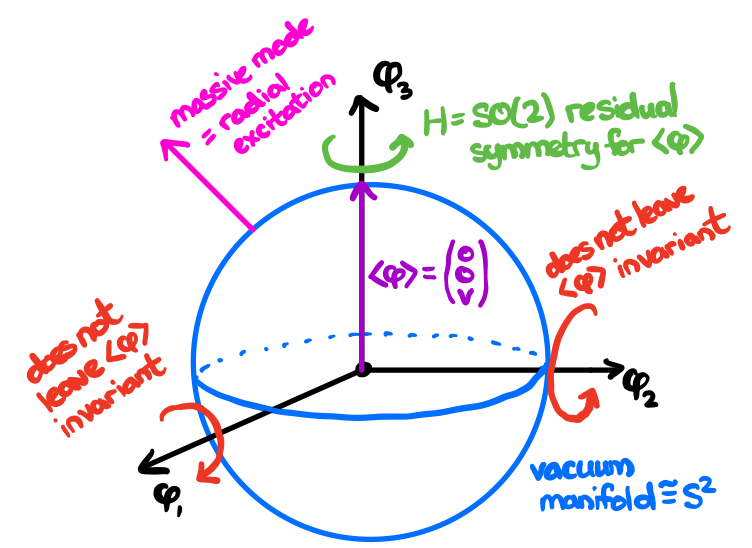
\includegraphics[width = 0.5\textwidth]{linear_sigma_ssb}
	\caption{Linear sigma model for $N = 3$. The vacuum manifold is the sphere of radius $v^2$, and the two 
	broken generators correspond to the red rotations, one around the $\phi_1$ axis and another around the $\phi_2$ axis. 
	These broken generators (Goldstone bosons) rotates the vev $\langle\phi\rangle$ around the vacuum manifold-- as such, 
	the Goldstones must be massless excitations, because every state on the sphere has the same energy.
	The residual symmetry is $H = SO(2)$, which corresponds to rotation about the $\phi_3$ axis and rotates the vev 
	$\langle\phi\rangle$ into itself.}~
	\label{fig:linear_sigma}
\end{figure}

In the case of the linear $\sigma$ model with $N = 3$, minimization of $\mathcal L$ implies that the ground state must have 
$|\langle\phi\rangle|^2 = v^2$. This defines the \textbf{vacuum manifold}, which is the subspace of states $\phi_0$ which 
may be taken as a valid ground state. In our model, the vacuum manifold consists of all vectors $\begin{pmatrix} \phi_0^1 & 
\phi_0^2 & \phi_0^3 \end{pmatrix}$ which have $\phi_0^i \phi_0^i = v^2$, i.e. the vacuum manifold is diffeomorphic to 
$S^2$, as shown in Figure~\ref{fig:linear_sigma}.

In Figure~\ref{fig:linear_sigma}, the Goldstone modes correspond to the broken generators: rotations about the $\phi_1$ and 
$\phi_2$ axes. Massive modes will correspond to anything that moves us off the sphere, which is the vacuum manifold. 
Note that the physics does not depend on the choice of $\langle\phi\rangle$. Suppose instead we had picked the vev 
$\langle\phi\rangle$ to lie somewhere else on the vacuum manifold, say along the $\phi_1$ direction, the broken generators 
would then correspond to $\phi_2$ and $\phi_3$ rotations. We would still get two Goldstone bosons, one from each of these 
rotations, and the residual symmetry would remain $H = SO(2)$, this time from rotations about $\phi_1$. 

Since each Goldstone boson is massless, it only has derivative couplings in the Lagrangian and its current matrix elements 
can be determined up to a scale factor. This means that we can write:
\begin{equation}
	\langle 0 | j_\mu^a(x) | \pi^b(p)\rangle = -i f_\pi \delta^{ab} p_\mu e^{-ipx}\neq 0
\end{equation}
where $f_\pi$ is some constant that determines the scale of the symmetry breaking, and $j_\mu^a$ are the broken currents 
corresponding to the spontaneously broken symmetry. The $\delta^{ab}$ comes in because we are always allowed to 
diagonalize this matrix. Intuitively, \textbf{this equation says that the broken symmetry current $j_\mu^a$ has the quantum numbers of 
$\pi^a$; it can connect the vacuum $| 0 \rangle$ with the one boson state $|\pi^a(x)\rangle$}. 

Here is some additional intuition for why $\pi^a$ can only have derivative couplings. At its most basic level, the Goldstone modes 
are defined by parameterizing the quotient space $G / H$. This means that if we shift $\pi^a$ as $\pi^a\mapsto \pi^a + f_\pi \theta^a$, 
then we must move around $G / H$; since $G$ is the original symmetry of $\mathcal L$ before SSB, this means that \textbf{the 
Lagrangian for $\pi^a$ must be invariant under shift symmetry}. Moving ourselves around the vacuum manifold changes the 
ground state, but it costs no energy, i.e. it is mediated by the massless Goldstone modes. This means that any Lagrangian we 
write down for $\pi^a$ must have this shift symmetry, and hence it can only contain derivative terms for $\pi$ because a 
constant term would not necessarily be invariant under shift symmetry.

\subsection{The 1PI effective action}

Our analysis up to now has been done in the classical limit, where the vev of $\phi$ is computed at first order without 
loop corrections. To include quantum effects, we must discuss the \textbf{1PI effective action}. This will not change the 
results of the previous section, but to see this one must work through the details. 

\subsection{$U(1)$ abelian Higgs model}

In the SM, the Goldstone modes do not appear as free massless particles. This is because they are absorbed into the degrees 
of freedom of other particles; we say they \textbf{the Goldstone modes are eaten by the gauge bosons}. This is typically 
illustrated with the $U(1)$ abelian Higgs model, in which there is a charged scalar Higgs boson and a massless gauge 
field. The basic Lagrangian is
\begin{equation}
	\mathcal{L} = -\frac{1}{4} F_{\mu\nu} F^{\mu\nu} + (D_\mu\phi)^\dagger (D^\mu\phi) - \mu^2\phi^*\phi + \frac{\lambda}{2}
	(\phi^*\phi)^2.
\end{equation}
We see that Higgs $\phi$ couples to the photon through $D_\mu\phi$, as $D_\mu = \partial_\mu - ig A_\mu$. The potential 
$V(\phi)$ is chosen so that there is spontaneous symmetry breaking, i.e. so that it has a minimum at $|\langle\phi\rangle|^2 = 
v^2 = \mu^2 / \lambda\neq 0$. When the Higgs field $\phi$ takes on its vev, we expand it as before as 
\begin{equation}
	\phi = \phi_0 + \frac{1}{\sqrt 2}(\phi_1(x) + i\phi_2(x)).
\end{equation}
When this expansion is plugged into the Lagrangian, we see that it generates a gauge invariant mass term for the photon, 
as well as a coupling between the $\phi_2$ field and $A_\mu$:
\begin{equation}
	\mathcal{L}\supset (D_\mu\phi)^\dagger (D^\mu\phi) = \frac{1}{2}(\partial_\mu\phi_1)^2 + \frac{1}{2}(\partial_\mu\phi_2)^2 
	 + \sqrt{2} e \phi_0 A^\mu\partial_\mu\phi_2 + e^2\phi_0^2 A_\mu A^\mu + \textnormal{higher order}
\end{equation}
We can use gauge freedom to rotate to a gauge where $\phi$ is purely real, and $\phi_2$ vanishes; this is called \textbf{unitary 
gauge}, and it removes the Goldstone boson completely. We can also identify the mass of the photon:
\begin{equation}
	m_A^2 = 2e^2\phi_0^2
\end{equation}
which is related to the coupling and the scale of symmetry breaking. 

An important question to ask is how exactly the Goldstone boson vanishes-- the field $\phi$ carries one degree of freedom, 
as it has a real and imaginary component but we can rotate between them using the $U(1)$ gauge freedom in our theory. 
This degree of freedom does not disappear, but is rather transferred to the gauge field $A_\mu$ when it is eaten. Recall that 
a massless vector field has two degrees of freedom (both transverse polarizations) and a massive vector field has three 
degrees of freedom (both transverse, one longitudinal polarizations). As the final theory has a massive vector field, the 
extra degree of freedom must have come from somewhere, and we can identify where exactly it came from. The three 
degrees of freedom contained by the massive $A_\mu$ field come from the two degrees of freedom in the massless 
$A_\mu$ field before symmetry breaking, and an additional degree of freedom from the Goldstone mode it ate!

Another parameterization we can use for this model is to expand $\phi - \phi_0$ in polar coordinates:
\begin{equation}
	\phi(x) = \phi_0 + \frac{1}{\sqrt 2} \sigma(x) e^{\frac{i}{f_\pi} \pi(x)}
\end{equation}
where $\sigma(x)$ and $\pi(x)$ are real fields and $f_\pi$ is a normalization (which will later be interpreted as the pion decay 
constant). The advantage of this parameterization is that it makes the different modes in the theory quite obvious. We can see 
that $\sigma(x)$ changes the norm of $\phi$ and perturbing $\sigma$ will move our field out of the potential (in the Mexican 
hat, this moves us out of the well). This means the $\sigma$ mode should be massive, because moving it costs energy. 
On the other hand, the $\pi$ field moves us along the bowl of the hat, and costs no energy at all. This can also be seen because 
$\mathcal L$ is invariant under phase rotations; a change in $\pi$ will move us between ground states in the vacuum manifold, 
but it will leave the Lagrangian invariant. 

This also makes it obvious why the Goldstone mode $\pi(x)$ can only have derivative terms. Since $\pi$ is the massless Goldstone 
mode, the Lagrangian \textit{must have shift symmetry} $\pi\mapsto \pi + f_\pi\theta$. This is a generic feature of spontaneous 
symmetry breaking. This shift symmetry means that we cannot have a non-derivative coupling, because if we did then the coupling 
would not be invariant under shifts. Thus $\pi$ can only couple to other fields as $\partial_\mu\pi$, which holds for a general 
SSB pattern.

\subsection{The Standard Model Higgs sector}

In the full Standard Model, the Higgs mechanism works in much the same way, just with extra quantum numbers. Recall 
Lagrangian for the Higgs sector is:
\begin{equation}
	\mathcal{L}_\mathrm{Higgs} = D_\mu H D^\mu H^\dagger + \mu^2 H^\dagger H - \lambda (H^\dagger H)^2
\end{equation}
where the Higgs transforms in the representation $\bf (1, 2)_{\frac{1}{2}}$ of $SU(3)\times SU(2)_L\times U(1)_Y$. Because 
the Higgs is a complex doublet, it has 3 degrees of freedom: 4 dof are from $H$ being a complex 2 dimensional vector, and 
one dof is subtracted off by gauge freedom. Therefore, the Higgs can give mass to three gauge bosons in the Standard Model; 
it will give mass to the $W^\pm$ and $Z$ bosons. 

From the Higgs potential, we find the Higgs must take the vev $H_0^\dagger H_0 = \frac{v^2}{2} = m^2 / 2\lambda$, where 
here $v$ is the magnitude of the Higgs vev which determines the scale of symmetry breaking:
\begin{equation}
	v = \sqrt{\frac{\mu^2}{\lambda}}
\end{equation}
Note that different conventions may have $v = \sqrt{2\mu^2 / \lambda}$ instead. We can choose an orientation for the Higgs vev 
by thinking about gauge freedom. We have a $SU(2)\times U(1)$ gauge theory, and we can write an arbitrary field in the fundamental 
as:
\begin{equation}
	H(x) = \exp\left( i\alpha^a(x) t^a + i b(x)\right)\begin{pmatrix} 0 \\ \phi(x) \end{pmatrix}
\end{equation}
with $\alpha^a$ and $b$ real, and $\phi(x)$ a real scalar field (note the $SU(2)$ piece allows us to move $\phi$ to the lower component, and 
the $U(1)$ piece allows us to perform a phase rotation and make $\phi$ real). Making the gauge transformation $H\mapsto e^{-i\alpha^a t^a - ib}$, we 
can therefore represent $H(x)$ with a real scalar field in the second component; this is called \textbf{unitary gauge}\footnote{Some books will take the 
Higgs to be in the first component. This changes a lot of charge conventions, and is perfectly fine to do, but you need to be consistent about 
whether the physical Higgs field lives in the top or not.}. This gives us the vev:
\begin{equation}
	\langle H \rangle = H_0 = \frac{1}{\sqrt 2}\begin{pmatrix} 0 \\ v \end{pmatrix}
\end{equation}
and using our parameterization we can perturb $H(x)$ around the vev,:
\begin{equation}
	H = \frac{1}{\sqrt 2} \begin{pmatrix} 0 \\ v + h(x)\end{pmatrix}
\end{equation}
Here $h(x)$ is the \textbf{physical Higgs field}: it is a real scalar field with hypercharge $\frac{1}{2}$. 

After expanding the kinetic term for $H$ with this parameterization we find the following terms in the Lagrangian:
\begin{equation}
	\mathcal L_\mathrm{Higgs}\supset D_\mu H D^\mu H^\dagger \supset \frac{g^2 v^2}{8} \left[\left(W_\mu^1\right)^2 + 
	\left(W_\mu^2\right)^2 + \left(\frac{g'}{g} B_\mu - W_\mu^3\right)^2\right]
\end{equation}
This expansion suggests (as is consistent with the argument earlier) that three of the vector bosons gain mass. The first 
two are linear combinations of the $W_\mu^1$ and $W_\mu^2$ fields:
\begin{equation}
	W_\mu^\pm := \frac{W_1 \mp i W_2}{\sqrt 2}
\end{equation}
so that the full gauge boson looks like:
\begin{equation}
	W_\mu^a t^a = \frac{1}{2} \begin{pmatrix} W_\mu^3 & \sqrt 2 W_\mu^+ \\
	\sqrt 2 W_\mu^- & W_\mu^3 \end{pmatrix}
\end{equation}

The third field which gains mass is a linear combination of $B_\mu$ and $W_\mu^3$ which is obtained through rotating 
these states with a unitary rotation into the fields $A_\mu$ (the \textbf{photon} field) and $Z_\mu$ (the \textbf{Z boson} field):
\begin{equation}
	\begin{pmatrix} A_\mu \\ Z_\mu \end{pmatrix} = 
	\begin{pmatrix} 
		\cos\theta_w & \sin\theta_w \\
		-\sin\theta_w & \cos\theta_w
	\end{pmatrix}
	\begin{pmatrix} B_\mu \\ W_\mu^3\end{pmatrix}
\end{equation}
The angle $\theta_w$ is called the \textbf{weak mixing angle} or the \textbf{Weinberg angle}, and has been determined 
experimentally to be about:
\begin{equation}
	\sin^2\theta_w \approx 0.223
\end{equation}
By comparing our expansion of the Lagrangian to the $Z_\mu$ field, we can read off an expression relating the coupling 
constants to the weak mixing angle:
\begin{align}
	\cos\theta_w = \frac{g}{\sqrt{g^2 + (g')^2}} && \tan\theta_w = \frac{g'}{g}
\end{align}

We can now explicitly see the relations between the masses of the $W$ and $Z$ bosons to the other SM parameters:
\begin{equation}
	\mathcal{L}_\mathrm{Higgs}\supset \left(\frac{gv}{2}\right)^2 \left(W_\mu^- W^{-\mu} + W_\mu^+ W^{+\mu}\right) + \left(\frac{v\sqrt{g^2 
	+ (g')^2}}{2}\right)^2 Z_\mu Z^\mu
\end{equation}
and so the gauge bosons have the following masses:
\begin{align}
	m_W = \frac{gv}{2} && m_Z = \frac{v}{2}\sqrt{g^2 + (g')^2}
\end{align}
and \textbf{their mass ratio is exactly determined by the gauge couplings}:
\begin{equation}
	\frac{m_W}{m_Z} = \frac{g}{\sqrt{g^2 + (g')^2}} = \cos\theta_w
\end{equation}

Now we turn to the final gauge boson, $A_\mu$, which generates the electromagnetic $U(1)$ symmetry seen at low energies. 
To determine the residual symmetry, we must find a generator of $SU(2)_L\times U(1)_Y$ under which the ground state 
of $H$ stays symmetric after symmetry breaking. This is equivalent to finding a linear combination $C_a t^a + D Y$ which annihilates the ground state, since the symmetry transformation is $e^{i(C_a t^a + DY)}\langle H \rangle = \langle H \rangle$. 

One can rewrite $B_\mu$ and $W_\mu^3$ in terms of $A_\mu$ and $Z_\mu$ by inverting the rotation, and the covariant 
derivative in the electroweak sector becomes:
\begin{equation}
	D_\mu = \partial_\mu -i \frac{g}{\sqrt 2} (W_\mu^+ t^+ + W_\mu^- t^-) + \left(\frac{g}{\cos\theta_w}\right) (t^3 - 
	Q\sin^2\theta_w) Z_\mu + e A_\mu Q~
	\label{eq:ew_cov}
\end{equation}
Note that here the generator $t^3 = \frac{1}{2}\sigma^3$ and the \textbf{electric charge} $e$ equals:
\begin{equation}
	e = g\sin\theta_w = \frac{gg'}{\sqrt{g^2 + (g')^2}}
\end{equation}
and $t^\pm$ are linear combinations of Pauli matrices:
\begin{align}
	t^\pm = \frac{1}{2}(\sigma^1 \pm i \sigma^2) && t^+ = \begin{pmatrix} 0 & 1 \\ 0 & 0 \end{pmatrix} &&
	t^- = \begin{pmatrix} 0 & 0 \\ 1 & 0 \end{pmatrix} 
\end{align}

% also do fermion masses
The spontaneous symmetry breaking of the Higgs directly gives the fermions mass via the Yukawa couplings. Looking back at the Yukawa 
sector:
\begin{equation}
	\mathcal L_\mathrm{SM}\supset -Y_{ij}^e \overline \ell_L^{i} H e_R^j - Y_{ij}^d \overline Q_L^i H d_R^j - Y_{ij}^u \overline Q^i \epsilon
	H^* u_R^j + \mathrm{h.c.}
\end{equation}
When the vev of the Higgs is inserted, $H\mapsto v / \sqrt 2$ and this gives a quadratic coupling between the correct fields to give 
$e$, $u$, and $d$ a Dirac mass. The Yukawa couplings must be diagonalized (which we will talk about in the section on the flavor sector) 
but this evidently generates fermion masses proportional to the vev $v$. We can see that the fermion masses are:
\begin{equation}
	m_f = \frac{1}{\sqrt 2} Y_f v
\end{equation}
where $Y_f$ is the diagonal component of the Yukawa matrix for fermion $f$, i.e. either $Y_{ii}^e$, $Y_{ii}^d$, or $Y_{ii}^u$ (with no sum). 
It also gives rise to three point couplings with two fermion lines and one Higgs line, which we will write out explicitly in the section on Higgs physics. 

\subsection{Custodial $SU(2)$}

Custodial $SU(2)$ refers to an accidental symmetry of the Standard Model which forces the mass relation:
\begin{equation}
	M_W = M_Z\cos\theta_W
\end{equation}

\subsection{Goldstone Equivalence Theorem}

We begin this section by discussing the polarizations of massive and massless spin 1 vector bosons. Suppose we have a massive vector boson 
moving in the $z$ direction, so $p^\mu = (E, 0, 0, p)$ with $E^2 = p^2 + m^2$. This vector boson has two transverse polarizations, which 
we will take to be left and right circular, $\epsilon_\mu^\pm$, and a longitudinal polarization $\epsilon_\mu^L$. These polarizations are 
explicitly given by:
\begin{align}
	\epsilon_\mu^\pm &= \frac{1}{\sqrt 2} \begin{pmatrix} 0 & 1 & \pm i & 0 \end{pmatrix} \\
	\epsilon_\mu^L &= \frac{1}{m} \begin{pmatrix} p & 0 & 0 & E \end{pmatrix}
\end{align}
where we note that the polarizations satisfy $\epsilon^L\cdot p = 0$ and have norm $\epsilon_\mu \epsilon^\mu = -1$. Furthermore, 
in the high energy limit $p^2 >> m^2$, the longitudinal polarization approaches the momentum divided by the mass, $\epsilon_\mu^L
\rightarrow p^\mu / m$. 

Suppose that we originally had a theory of massless gauge bosons which are given mass by the Higgs mechanism; each gauge boson 
eat the real scalar Higgs field (in the SM this is the $W^\pm$ and the $Z$) and gain an additional degree of freedom which becomes 
a longitudinal polarization. The \textbf{Goldstone equivalence theorem} states that at high energies, $p^2 >> m^2$, we can treat 
this longitudinal polarization as the original Goldstone boson. Amplitudes in the un-Higgsed theory agree with those in the Higgsed 
theory up to subleading terms of order $m_h / E$ or $m_V / E$. 

This is best illustrated as an example in top quark decay. The top quark has mass $m_t\approx 175\;\mathrm{MeV}$, and it decays primarily 
through a $b$ quark and $W^+$, $t\rightarrow b W^+$. Since this is a high energy process, we can apply the Goldstone equivalence theorem. 
The $t\rightarrow b W^+$ matrix element goes as $\frac{g}{\sqrt 2} V_{tb} \epsilon_\mu^W \overline u(b) \gamma^\mu P_L u(t)$, and we can see 
how the transverse and longitudinal components look. Since the transverse polarization is order 1 and the longitudinal polarization goes as $p^\mu / m$, 
we see the relative contribution of a transverse or longitudinal $W$ boson to the scattering amplitude goes as (using that spinors go as $\sqrt{p\cdot\sigma}$, so 
$u(t)\sim \sqrt{m_t}$ and $u(b)\sim \sqrt{E_b}$ in the rest frame of the top):
\begin{align}
	\mathcal M_{\mathrm{transverse}}&\sim g V_{tb} \sqrt{m_t E_b}\sim g m_t \\
	\mathcal M_{\mathrm{longitudinal}}&\sim g V_{tb} \sqrt{m_t E_b} \frac{E_W}{m_W}\sim g \frac{m_t^2}{m_W}
\end{align}
where at first order all the energies are at the same scale, $E_b\sim m_t\sim m_W$. 

The part of this computation that illustrates the Goldstone equivalence theorem is to examine how the positively charged component of the 
Higgs field, $h^+$, couples to the top and bottom quarks when we are not in unitary gauge. In this case it provides a coupling between the 
top and bottom quarks proportional to $Y_t$ (the diagonal component of the $Y_u^{ij}$ matrix for the top quark), and so the amplitude is:
\begin{equation}
	\mathcal M_\mathrm{Goldstone} = \mathcal M(t\rightarrow b \pi^+)\sim y_t \overline u(t) u(b)\sim Y_t m_t
\end{equation}
where we make the same order of magnitude estimates as before of $\overline u(t) u(b)\sim \sqrt{m_t E_b}\sim m_t$. Recalling that the 
mass of the top and the top's Yukawa are directly proportional as $Y_t = \frac{m_t}{v}$, we see that:
\begin{equation}
	\mathcal M_\mathrm{Goldstone}\sim Y_t m_t \sim \frac{m_t^2}{v}\sim g\frac{m_t^2}{m_W} = \mathcal M_\mathrm{longitudinal} + \mathcal O\left(\frac{m_W^2}{m_t^2}\right)
\end{equation}
since the $W$ mass is equal to $m_W = \frac{gv}{2}$. The order $(m_W / m_t)^2$ corrections can be shown by actually working through the 
computation carefully. This is explicitly a statement of the Goldstone equivalence theorem: \textbf{at high energies ($E >> m_W$), the 
longitudinal degree of freedom of a massive vector boson which gains its mass through SSB can be replaced with the original Goldstone 
boson}. The theory essentially ``forgets" that the Goldstone boson was eaten, and it decouples into its own mode which has the same 
physics as the longitudinal gauge boson. 

Since the Goldstone bosons couple directly to the fermions in the Standard Model, the Goldstone equivalence theorem can be used to 
simplify computations. We saw in this case that using the Goldstone coupling to the quarks gave a much simpler invariant matrix element 
than going through the full vector boson. Furthermore, at high energies the longitudinal degree of freedom of the vector boson typically 
dominates the computation because it scales as $p^\mu / m\sim E / m$, so the ability to substitute out the longitudinal polarization for a 
scalar particle is quite useful in many high-energy computations. 

\subsection{Higgs physics}

We'll talk about the Higgs further when we discuss colliders, but the Higgs often comes up in questions about decay rates or production. 
The Higgs couples to fermions via its Yukawa interactions, and we can expand the Higgs out in unitary gauge $H = \frac{1}{\sqrt 2}
\begin{pmatrix} 0 \\ v + h(x) \end{pmatrix}$ to determine its Feynman rules:
\begin{align}
	\mathcal L_\mathrm{Yuk} &= -Y^e_{ij} \overline\ell_L^i H e_R^j - Y_{ij}^d \overline Q_L^i H d_R^j - Y_{ij}^u \overline Q_L^{ai} \epsilon_{ab} H^{\dagger b} u_R^j + h.c. \\
	&\supset -\frac{1}{\sqrt 2}(v + h)\left[Y^e_{i} \overline e_L^i e_R^i + Y^d_i d_L^i d_R^i + Y_i^u u_L^i u_R^i \right] + h.c.
\end{align}
where in the second line we have assumed we are in the mass basis so the Yukawas are diagonal. We know the terms proportional to $v$ 
give the fermions a mass equal to $m_f = \frac{1}{\sqrt 2} v Y_f$, where $v = 247\;\mathrm{GeV}$, and it is useful to keep in mind that the 
\textit{Yukawa coupling and the fermion mass are directly proportional}. There is thus a 3-point coupling between a Higgs $h$ and a 
fermion-antifermion pair $h\overline\psi\psi$ which is proportional to its mass:
\begin{equation}
	\begin{gathered}
\feynmandiagram [small, horizontal=a to b] {
	  a [particle=\(\pi\)] -- [scalar, edge label=\(h\)] b,
	  f1 [particle=\(f\)] -- [anti fermion] b -- [anti fermion] f2 [particle=\(\overline{f}\)]
	};
	\end{gathered} = \frac{1}{\sqrt 2} Y_f = \frac{m_f}{v}
\end{equation}

There are also couplings of the Higgs with the gauge bosons. These are easily determined by acting the covariant derivative on the Higgs, and 
you can confirm that the mass terms in front of the gauge bosons reproduce their usual masses. Recall that for a complex field the mass term 
is $-m^2 \phi^*\phi$ and for a real field it is $\frac{1}{2} m^2 \phi^2$. We have:
\begin{align}
	\mathcal L\supset |D_\mu H|^2\supset -m_W^2 \left(1 + \frac{h}{v}\right) W_\mu^+ W^{\mu +} - \frac{1}{2} m_Z^2 Z_\mu Z^\mu
\end{align}
which produces couplings of the form $h WW$ and $hhWW$.

% Trick to remember the couplings: replace mass terms with v(1 + \frac{h}{v})
These couplings aren't pretty, but there's an easy way to remember them. The Higgs term produces the mass for the gauge bosons and the 
fermions, so we can use this knowledge to our advantage. Since in unitary gauge the bottom component comes as $\frac{1}{\sqrt 2} v(1 + 
\frac{h}{v})$ and the $\frac{v}{\sqrt 2}$ part of the term generates the mass, we can simply add in $\frac{h}{v}$ to the relevant mass term 
to get the exact form of the coupling, because this term always comes as $1 + \frac{h}{v}$. Explicitly, this is the prescription:
\begin{equation}
	m\mapsto m\left(1 + \frac{h}{v}\right)
\end{equation}
made for each mass term. For fermions, this term is $-m_f\overline\psi_f\psi_f$, for the $W$ it is $-m_W^2 W_\mu^+ W^{\mu -}$, and for the $Z$ it 
is $-\frac{1}{2} m_Z^2 Z_\mu Z^\mu$. 

% Higgs decay products: h --> fermions, h --> gauge bosons. The most common decay product of the Higgs is to a b \bar{b} pair-- explain why
Let's talk about the decay of the Higgs. We've just discussed the couplings of the Higgs, so we can see it could potentially decay either 
into a diagonal pair of fermions or gauge bosons. We know $m_H\approx 125\;\mathrm{GeV}$, so the gauge bosons are not allowed by 
energy conservation ($2m_W\approx 169$ GeV and $2m_Z\approx 182$ GeV) and neither is a top-antitop pair ($2 m_t\approx 350\;\mathrm{GeV}$). 
This means the Higgs will only decay to fermions which are lighter than the top quark. Furthermore, we can already see what its most frequent 
decay mode is. The Higgs couples with the strength of the appropriate Yukawa coupling, which is related to the mass as $\frac{m_f}{v}$. 
Therefore the most massive fermion left will couple the strongest to the Higgs, so \textit{the Higgs will decay most frequently to a $b\overline b$ 
pair}. 

Let's compute this decay rate to a fermion $f$ for practice. The amplitude for the process $h\rightarrow f\overline f$ is:
\begin{equation}
	\mathcal M(h\rightarrow f\overline f) = -i \frac{m_f}{v} \overline u(f) v(f) \implies \overline{|\mathcal M|^2}\approx \frac{m_f^2}{v^2}\Lambda^2
\end{equation}
The mass scale $\Lambda$ could be any of $m_f$, $v$, or $m_h$; since the Higgs mass is the only one which has not come into play 
yet and should clearly come into play in the final decay width, let's use that. We then have the approximate cross section:
\begin{align}
	\Gamma(h\rightarrow f\overline f) &\approx \frac{1}{2m_h} \frac{(2\pi)^4}{(2\pi)^6}\frac{1}{2^2} (2\pi) \overline{|\mathcal M|^2} \\
	&= \frac{1}{16\pi}\frac{m_f^2 m_h}{v^2} \left(1 - \frac{4 m_f^2}{m_h^2}\right)^2
\end{align}
This is typically written in terms of the Fermi coupling $\frac{G_F}{\sqrt 2} = \frac{g^2}{8 m_W^2} = \frac{1}{2v^2}$, using the $W$ mass relations.
Note that the mass of the fermions also depends on the renormalization scale. We will typically choose $m_f$ to be the $\overline{\mathrm{MS}}$ 
mass at scale $\mu = m_h$. For the quarks, there is a large amount of running:
\begin{equation}
	m_f(Q) = m_f(m_f)\left(\frac{\alpha_s(Q)}{\alpha_s(m_f)}\right)^{4 / \beta_0}
\end{equation}
Note the predominant running is from the strong coupling, which is why only quarks are affected by this; lepton masses 
can be inserted into Eq.~(\ref{eq:higgs_width}) without needing to renormalize them. We can see that the mass values will decrease 
after renormalization, since $\alpha_s(Q) < \alpha_s(m_f)$ due to asymptotic freedom. The renormalized $\overline{\mathrm{MS}}$ 
mass of the $b$, for example, is about 3 GeV at this scale. 
% https://indico.mitp.uni-mainz.de/event/22/attachments/900/959/Peskin-2.pdf

% Gluon fusion and production at colliders


\newpage
\section{Flavor Sector}

\subsection{The CKM Matrix}

The CKM matrix measures the difference between the mass eigenstates of the Standard Model and its flavor eigenstates. The way we have 
wrote down the Standard Model so far is using the so-called \textbf{flavor eigenstates} for the fermions, where the quark and lepton flavors 
directly couple to one another and to the gauge bosons. However, in the flavor basis the Yukawa couplings $Y_{ij}$, Eq.~(\ref{eq:yukawa}), 
are not necessarily diagonal. Since the Yukawas give the fermions mass after electroweak symmetry breaking, the \textbf{mass eigenstates}
for fermion flavors are obtained by diagonalizing the Yukawa couplings and explicitly determining how much mass each quark / lepton gains. 
For now, we will only consider the quarks: when neutrino mass is included in the Standard Model, this procedure can be followed to 
obtain the \textbf{PMNS matrix}, which describes the flavor $\leftrightarrow$ mass mixing of the electron and neutrino. After symmetry 
breaking the Yukawa couplings for the quarks become:
\begin{equation}
	\mathcal L_\mathrm{SM}\supset - \frac{v}{\sqrt 2} Y_{ij}^d \overline d_L^i d_R^j - \frac{v}{\sqrt 2} Y_{ij}^u \overline u_L^i u_R^j + \mathrm{h.c.}
\end{equation}

To diagonalize the Yukawa couplings, we apply the singular value decomposition (SVD) to each matrix $Y_{ij}$ as:
\begin{align}
	Y_{ij}^d = U_d M_d K_d^\dagger && Y_{ij}^u = U_u M_u K_u^\dagger
\end{align}
where the $K$ and $U$ matrices are unitary and $M_u$ is diagonal. Upon inserting this into the Yukawas, it is apparent that we can 
redefine the quark basis $\{u^i, d^j\}$ so that the mass terms become explicit and the new quark basis only couples to itself 
diagonally. We see that:
\begin{align}
	\mathcal L_\mathrm{mass} &= - \frac{v}{\sqrt 2} \left[ \overline d_L U_d M_d K_d^\dagger d_R + u_L U_u M_u K_u^\dagger u_R  \right]
	+ \mathrm{h.c.} \\
	&\mapsto -m_j^d \overline{d}_L^{j} d_R^j - m_j^u \overline u_L^j u_R^j
\end{align}
where in the second line we have made the field redefinition:
\begin{align}
	d_L\mapsto U_d d_L && u_L\mapsto U_u u_L && d_R\mapsto K_d d_R && u_R\mapsto K_u u_R
\end{align}
and the masses are equal to $m_j^d = diag(\frac{v}{\sqrt 2} M_d)$ and $m_j^u = diag(\frac{v}{\sqrt 2} M_u)$. This new basis for the 
quarks is known as the \textbf{mass basis}, and upon this basis transformation each quark has $u^i$ and $d^j$ has a definite mass. 

This change of basis does not affect the SM Lagrangian much: it is only felt in the couplings to the $W$ boson. For any diagonal coupling 
between $u$ and $\overline u$ (or $d$ and $\overline d$), assuming there is no coupling between different flavors, the rotation just 
cancels itself out (i.e. in $\overline Q_L i\slashed \partial Q_L = \overline u_L^i i\slashed \partial u_L^i + (u\leftrightarrow d)$ the diagonal 
couplings mean that $U_u$ and $U_u^\dagger$ annihilate one another). The only place where the rotations do not cancel one another out 
is when we separately rotate the up and down quarks, i.e. in the off-diagonal $W$ couplings. Looking at our previous expression for 
$D_\mu$ after electroweak SSB, the off-diagonal components in $SU(2)_L$ are changed by the field redefinition:
\begin{align}
	\mathcal L_\mathrm{SM}&\supset\overline Q_L i\slashed D Q_L\supset \frac{g}{\sqrt 2} \begin{pmatrix} \overline u_L & \overline d_L 
	\end{pmatrix} \begin{pmatrix} 0 & \slashed{W}^+ \\ \slashed{W}^- & 0 \end{pmatrix} \begin{pmatrix} u_L \\ d_L \end{pmatrix}
	= \frac{g}{\sqrt 2} \left( \overline u_L \slashed W^+ d_L + \overline d_L \slashed W^- u_L\right) \\
	&\mapsto \frac{g}{\sqrt 2} \left( \overline u_L^i \slashed W^+ (U_u^\dagger U_d)^{ij} d_L^j + \overline d_L^i \slashed W^- (U_d^\dagger 
	U_u)^{ij} u_L^j \right)
\end{align}
This combination of matrices is not necessarily unity, and is known as the \textbf{Cabibbo-Kobayashi-Maskawa (CKM) matrix}:
\begin{equation}
	V_\mathrm{CKM} := U_u^\dagger U_d = \begin{pmatrix} V_{ud} & V_{us} & V_{ub} \\
	V_{cd} & V_{cs} & V_{cb} \\
	V_{td} & V_{ts} & V_{tb}
	 \end{pmatrix}.
\end{equation}
A helpful way to remember how the CKM matrix enters the $W$ couplings is to remember that we parameterize it as $V_{ud}$, i.e. with 
an up-type flavor on the left and a down-type flavor on the right, and that it must couple the flavors together as $\overline u V_{ud} d$ or 
$\overline d V^\dagger_{du} u$. Written out explicitly, the CKM matrix appears only in the mass basis and only in the $W$ couplings:
\begin{equation}
	\mathcal L_\textnormal{mass basis} \supset \frac{g}{\sqrt 2} \left( \overline u_L^i \slashed W^+ V_\mathrm{CKM}^{ij} d_L^j + 
	\overline d_L^i \slashed W^- (V_\mathrm{CKM}^\dagger)^{ij} u_L^j \right)
\end{equation}
There is no corresponding mixing matrix for the $K$ matrices, since $u_R$ and $d_R$ are never coupled together as they don't interact 
via $SU(2)_L$. 

The CKM matrix is a $3\times 3$ unitary matrix, and hence should have 9 degrees of freedom, 3 real rotation angles and 6 phases. 
However, we can use phase rotations to move these degrees of freedom around. For each quark $q_L^i$ (here $q = u, d, s, ...$), we can 
redefine the field via a phase rotation $q_L^i\mapsto e^{i\alpha_i} q_L$ without changing the Lagrangian. This allows us to soak up most of 
the phases into redefined quark fields without changing the physics. When we rotate a $u$-type quark field, we rotate the corresponding 
row of $V_\mathrm{CKM}$, and a $d$-type rotation changes a column of $V_\mathrm{CKM}$. If we perform an axial rotation on the fields, 
$u_L^i\mapsto e^{i\Delta} u_L^i$ and $d_L^i\mapsto e^{-i\Delta} d_L^i$, we see that $V_\mathrm{CKM}\mapsto e^{i\Delta} e^{-i\Delta} 
V_\mathrm{CKM} = V_\mathrm{CKM}$ is invariant under this rotation. Thus \textit{we can absorb $6 - 1 = 5$ phases into phase redefinitions 
of the quark fields}, where the one degree of freedom we cannot absorb is because we cannot perform axial phase rotations and change 
the CKM matrix. We therefore see that \textbf{the CKM matrix has 4 degrees of freedom: 3 real angles $\theta_{12}, \theta_{13}$, and 
$\theta_{23}$, and one irremovable phase $\delta$}. 
The phase $\delta$ is called \textit{irremovable} because we can use phase redefinitions on the quark fields, $u_i\mapsto e^{i\alpha} u_i$ 
(or the same for $d$) to move around pieces of the CKM matrix, but we will always be left with one phase which cannot be removed. 

The most common parameterization of the CKM matrix is via these four parameters. We can write $V_\mathrm{CKM}$ as:
\begin{equation}
	V_\mathrm{CKM} = \begin{pmatrix} 
		1 & 0 & 0 \\ 0 & \cos\theta_{23} & \sin\theta_{23} \\ 0 & -\sin\theta_{23} & \cos\theta_{23} 
	\end{pmatrix}
	\begin{pmatrix} 
		\cos\theta_{13} & 0 & e^{-i\delta} \sin\theta_{13} \\ 0 & 1 & 0 \\ e^{-i\delta} \sin\theta_{13} & 0 & \cos\theta_{13} 
	\end{pmatrix}
	\begin{pmatrix}
		\cos\theta_{12} & \sin\theta_{12} & 0 \\ -\sin\theta_{12} & \cos\theta_{12} & 0 \\ 0 & 0 & 1 
	\end{pmatrix}
\end{equation}
Another common parameterization for $V_\mathrm{CKM}$ is called the \textbf{Wolfenstein parameterization}, which is performed by noting 
the observable magnitudes of these angles. All the angles are relatively small, but $\theta_{13}$ and $\theta_{23}$ are $<< \theta_{12}$ 
(see the Appendix for exact numerical values). This allows one to write the matrix as:
\begin{equation}
	V_\mathrm{CKM} = \begin{pmatrix} 1 - \frac{\lambda^2}{2} & \lambda & \lambda^3 \\
	-\lambda & 1 - \frac{\lambda^2}{2} & \lambda^2 \\
	\lambda^3 & \lambda^2 & 1
	\end{pmatrix}
	\label{eq:wolfenstein}
\end{equation}
where $\lambda := \sin\theta_{12} = 0.22$.

\subsection{The unitary triangle and CP violation}

The unitary triangle is a helpful mnemonic device to derive constraints on elements of the CKM matrix. Since $V_\mathrm{CKM}$ is 
unitary, we have the condition that:
\begin{equation}
	V_\mathrm{CKM}^\dagger V_\mathrm{CKM} = 1 = V_\mathrm{CKM} V_\mathrm{CKM}^\dagger
\end{equation}
This implies that the rows / columns of $V_\mathrm{CKM}$ are orthonormal, which gives us 6 orthogonality conditions (3 for the rows and 3 
for the columns). For example, dotting the first row with the last row gives the most commonly used condition:
\begin{equation}
	V_{ud} V_{ub}^* + V_{cd} V_{cb}^* + V_{td} V_{tb}^* = 0 = \frac{V_{ud} V_{ub}^*}{V_{cd} V_{cb}^*} + \frac{V_{td} V_{tb}^*}{V_{cd} 
	V_{cb}^*} + 1~
	\label{eq:unitary_triangle}
\end{equation}
Pictorially, this equation can be represented as a triangle in the complex plane, where each leg represents one of the terms on the right-hand 
side of Eq.~(\ref{eq:unitary_triangle}). This is depicted in Figure~\ref{fig:unitary_triangle}. 
\begin{figure}[H]
	\centering
	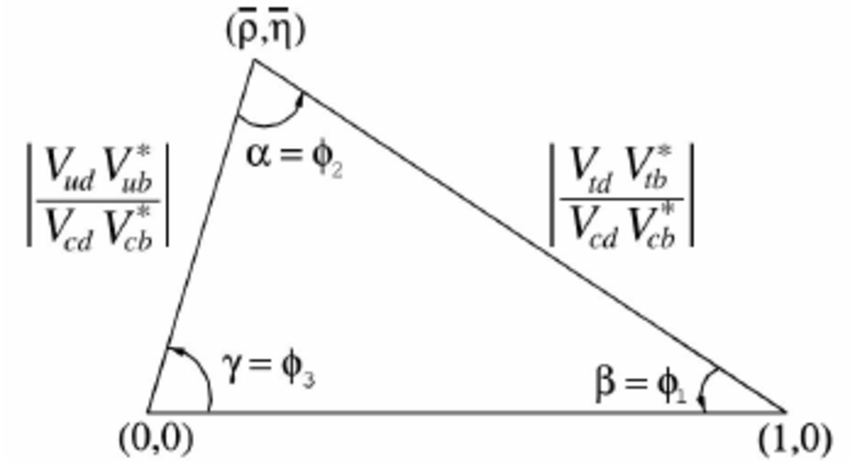
\includegraphics[width = 0.6\textwidth]{unitary_triangle}
	\caption{Representation of Eq.~(\ref{eq:unitary_triangle}) via the unitary triangle. The bottom leg has length 1 because of the 
	division by $V_{cd} V_{cb}^*$.}~
	\label{fig:unitary_triangle}
\end{figure}

A useful invariant that can be determined from this discussion is called the \textbf{Jarlskog invariant}, which is twice the area of the unitary 
triangle (without rescaling):
\begin{equation}
	J = 2(\mathrm{area}) = \mathbb Im\left[ V_{ud} V_{tb} V_{td}^* V_{ub}^* \right] = s_{12} s_{23} s_{13} c_{12} c_{23} c_{13}^2\sin\delta
\end{equation}
where $s_{ij} = \sin\theta_{ij}$ and $c_{ij} = \cos\theta_{ij}$. This is thus directly proportional to the phase $\delta$, and so provides a 
measure of the CP violation in the Standard Model. The Jarlskog invariant has been measured to be small:
\begin{equation}
	J = (2.96\pm 0.2) \times 10^{-5}
\end{equation}

I keep droning on and on about the irremovable phase because it directly implies CP violation in the electroweak sector. Under CP 
symmetry, $W^\pm\mapsto W^\mp$ and fermion bilinears go as 
\begin{align}
	\overline \psi_i\psi_j(\vec x, t)\mapsto \overline\psi_j\psi_i (-\vec x, t) && \overline\psi_i \slashed A \psi_j(\vec x, t)\mapsto 
	\overline\psi_j\slashed A\psi_i (-\vec x, t) \\
	\overline \psi_i\gamma_5 \psi_j(\vec x, t)\mapsto - \overline\psi_j\gamma_5\psi_i (-\vec x, t) && 
	\overline\psi_i \slashed A \gamma_5 \psi_j(\vec x, t)\mapsto \overline\psi_j\slashed A \gamma_5 \psi_i (-\vec x, t)
\end{align}
This implies that the rest of the Lagrangian is invariant, but the part with the CKM matrix 
transforms as:
\begin{align}
	\mathcal L\supset &\frac{g}{\sqrt 2} \left( \overline u_L^i \slashed W^+ V_\mathrm{CKM}^{ij} d_L^j + \overline d_L^i \slashed W^- 
	(V_\mathrm{CKM}^\dagger)^{ij} u_L^j \right) \\
	\xrightarrow{CP} &\frac{g}{\sqrt 2} \left(\overline d_L^j \slashed W^- 
	V_\mathrm{CKM}^{ji} u_L^i  +  \overline u_L^j \slashed W^+ (V_\mathrm{CKM}^\dagger)^{ij}  = d_L^i \right)
	= \frac{g}{\sqrt 2} \left( \overline u_L^i \slashed W^+ (V_\mathrm{CKM}^*)^{ij} d_L^j + \overline d_L^i \slashed W^- 
	(V_\mathrm{CKM}^T)^{ij} u_L^j \right)\nonumber
\end{align}
This makes it obvious that if $V_\mathrm{CKM}^* = V_\mathrm{CKM}$, then there is no CP violation and 
$\mathcal L_\mathrm{electroweak}$ is invariant under CP. On the other hand, \textbf{a complex CKM matrix $V_\mathrm{CKM}^*\neq 
V_\mathrm{CKM}$ directly implies CP violation in the electroweak sector}. 

The existence of CP violation in the electroweak sector allows us to actually put a constraint on the number of generations in the 
Standard Model. Suppose that there were only two generations in the Standard model, so the CKM matrix was a $2\times 2$ unitary matrix. 
In this case, $V_\mathrm{CKM}$ would have one rotation angle and 3 phases\footnote{For an $N\times N$ unitary matrix, the number of 
rotation angles is the dimension of $SO(N)$ and the number of phases is $dim(U(N)) - dim(SO(N))$, since phases make up the remaining 
generators.}. But, four quarks gives us $4 - 1 = 3$ phase rotations which will will affect the CKM matrix, and so in this case we can in fact 
remove all of the phases in $V_\mathrm{CKM}$ via phase rotations. \textbf{Therefore for CP to be violated in the electroweak sector, the 
Standard Model must have at least 3 generations}.

\subsection{Currents}

%J_\mathrm{CC, f}^{\mu} W_\mu^\pm

Currents are often useful for calculations in electroweak theory, so we will separate them out in this section. There are 
numerous different conventions which we discuss. The electroweak interaction Lagrangian (note this does not include 
the Higgs) is:
\begin{equation}
	\mathcal L_\mathrm{EW, int} = \sum_f \overline\psi_f i\slashed D\psi_f
\end{equation}
This looks extremely simple, but this is its most compact form. It is easiest to study interactions in this sector by expanding the 
Lagrangian out into currents which mediate the interactions. This is done by using Eq.~(\ref{eq:ew_cov}) and substituting in this 
expression for the covariant derivative, $D_\mu = \partial_\mu - \textnormal{(gauge couplings)}$. There are a few currents of interest.
First, the \textbf{charged currents}, which are the ones which couple to the $W$ bosons:
\begin{equation}
	\mathcal L\supset \frac{g}{\sqrt 2} \left( j^{\mu +}_\mathrm{CC} W_\mu^+ + j^{\mu -}_\mathrm{CC} W_\mu^-\right)
\end{equation}
The normalization strips off the coupling $g / \sqrt 2$ from the current, and ``CC" stands for the charged current. 
These currents separate into quark and lepton pieces. The lepton pieces are flavor-diagonal (they would not 
be if the PMNS matrix was introduced) and the quark pieces of the current are \textbf{flavor changing}, since quarks couple to the $W$ 
boson through the CKM matrix. The currents are:
\begin{align}
	j_{\textnormal{CC}}^{\mu +} &= \overline u^i \gamma^\mu V^{ij}_\mathrm{CKM} P_L d^j +  \overline\nu_e \gamma^\mu P_L e + \overline\nu_\mu 
	\gamma^\mu P_L \mu + \overline\nu_\tau \gamma^\mu P_L \tau \\
	j_{\textnormal{CC}}^{\mu -} &= \overline d^i \gamma^\mu (V_\mathrm{CKM}^\dagger)^{ij} P_L u^j + \overline e \gamma^\mu 
	P_L\nu_e + \overline \mu \gamma^\mu P_L \nu_\mu + \overline\tau \gamma^\mu P_L\nu_\tau = (j_\mathrm{CC}^{\mu +})^\dagger 
\end{align}
These currents are used as the basis for the 4-Fermi theory, which we will discuss in a few sections. Note that since they are left-handed 
currents, each fermion current comes in as a $V - A$ current, where $V$ is the vector current ($\overline\psi\gamma^\mu\psi$) and $A$ is 
the axial current ($\overline\psi\gamma^\mu\gamma_5\psi$) for a fermion $\psi$. 

The hadronic charged currents can be written as a linear combination of vector and axial currents in the chiral limit, 
Eq.~(\ref{eq:chiral_currents}). In the \textit{flavor basis}, the hadronic charged current connecting the up and down quarks can be written 
as a linear combination of the left-handed currents $j_L^{\mu 1}$ and $j_L^{\mu 2}$:
\begin{align}
	j_\mathrm{CC, had, flavor}^{\mu +} = \overline u \gamma^\mu P_L d = j_L^{\mu 1} + i j_L^{\mu 2} &&
	j_\mathrm{CC, had, flavor}^{\mu -} = \overline d \gamma^\mu P_L u = j_L^{\mu 1} - i j_L^{\mu 2} 
\end{align}

The neutral and electromagnetic currents can be written out through the fermion couplings to the Z boson and the photon:
\begin{equation}
	\mathcal L\supset \frac{g}{\cos\theta_w} j_\mathrm{NC}^{\mu} Z_\mu + e j_\mathrm{EM}^\mu A_\mu
\end{equation}
where ``NC" stands for \textbf{neutral current}. This gives us the expressions:
\begin{align}
	j_\mathrm{NC}^\mu &= \sum_f \left( \overline\psi_f \gamma^\mu t^3 P_L\psi_f - Q_f\sin^2\theta_w \overline\psi_f\gamma^\mu\psi_f 
	\right) \\
	j_\mathrm{EM}^\mu &= \sum_f Q_f \overline \psi_f \gamma^\mu\psi_f
\end{align}
where the sum on $f$ indexes all the fermion types in the SM. Each particle type has its own neutral current. For example, the $u$ and $d$ 
type quarks have the currents:
\begin{align}
	j_\mathrm{NC, u}^\mu = \overline u \gamma^\mu \left(\frac{1}{4} - \frac{2}{3}\sin^2\theta_w - \frac{1}{4}\gamma_5 
	\right) u && 
	j_\mathrm{NC, d}^\mu = \overline d \gamma^\mu \left(-\frac{1}{4} + \frac{1}{3}\sin^2\theta_w + \frac{1}{4} 
	\gamma_5 \right) d
\end{align}
Note that some conventions take another factor of $\frac{1}{2}$ out in the definition of $j_\mathrm{NC}^\mu$ to remove that factor 
from the left-handed projector, but here we will not do that.
% See Iain's notes, pg 95. Different convention from structure of the nucleon to write out the hadronic and leptonic currents

Another convention that is often used is to expand out the currents in the vector / axial basis, since we explicitly know the 
parameterization:
\begin{equation}
	\mathcal L\supset \frac{g}{\cos\theta_w} \sum_f \overline\psi_f \left(g_V^{(f)} \gamma^\mu - g_A^{(f)}
	\gamma^\mu\gamma_5\right) \psi_f
\end{equation}
where the axial and vector couplings for each flavor can be determined by matching this form to the neutral current:
\begin{align}
	g_V^{(f)} = \frac{1}{2} t^3_f - Q_f\sin^2\theta_w && g_A^{(f)} = \frac{1}{2} t^3_f
\end{align}
For some specific particles, we have:
\begin{align}
	g_V^{(u)} &= \frac{1}{4} - \frac{2}{3}\sin^2\theta_w && g_A^{(u)} = \frac{1}{4} \\
	g_V^{(d)} &= -\frac{1}{4} + \frac{1}{3}\sin^2\theta_w && g_A^{(d)} = -\frac{1}{4} \\
	g_V^{(e)} &= -\frac{1}{4} + \sin^2\theta_w && g_A^{(e)} = -\frac{1}{4}
\end{align}

\subsection{4 Fermi Theory}

The 4 Fermi theory is an effective theory of electroweak decay via $W$ bosons. This theory takes us to be working at an energy scale 
$p^2 << m_W^2, m_Z^2$ and integrates these bosons out of the theory. Recall the charged and neutral electroweak currents:
\begin{align}
	j_{\textnormal{CC}}^{\mu +} &= \overline u^i \gamma^\mu V^{ij}_\mathrm{CKM} P_L d^j +  \overline\nu_e \gamma^\mu P_L e + \overline\nu_\mu 
	\gamma^\mu P_L \mu + \overline\nu_\tau \gamma^\mu P_L \tau \\
	j_{\textnormal{CC}}^{\mu -} &= \overline d^i \gamma^\mu (V_\mathrm{CKM}^\dagger)^{ij} P_L u^j + \overline e \gamma^\mu 
	P_L\nu_e + \overline \mu \gamma^\mu P_L \nu_\mu + \overline\tau \gamma^\mu P_L\nu_\tau = (j_\mathrm{CC}^{\mu +})^\dagger 
	\\
	j_\mathrm{NC}^\mu &= \sum_f \left( \overline\psi_f \gamma^\mu t^3 P_L\psi_f - Q_f\sin^2\theta_w \overline\psi_f\gamma^\mu\psi_f \right)
\end{align}
These are, up to whatever convention is chosen for the couplings, the fermionic currents which couple to the massive vector bosons 
$Z_\mu$ and $W_\mu^\pm$. When these bosons are integrated out of the theory, we get the 4-Fermi Lagrangian:
\begin{equation}
	\mathcal L_{4F} = \frac{4 G_F}{\sqrt 2} \left(j_{\mathrm{CC},\,\mu}^+ \, j_\mathrm{CC}^{\mu -} + \cos^2\theta_w \, j_{\mathrm{NC},\,\mu}
	\,j_\mathrm{NC}^\mu\right)
\end{equation}
Note that in Schwartz, there is no $\cos\theta_w$ because we have defined our currents with an extra factor of $1 / \cos\theta_w$. 
This is historically how the Standard Model was predicted: Fermi used this theory to describe beta decay, and eventually the four-Fermi 
theory found a UV completion in the Standard Model. 

The 4 Fermi theory is nonrenormalizable because the operators it describes are dimension 6 operators (as the fermion fields have $[\psi] = 
3 / 2$). Therefore, the coupling has mass dimension $[G_F] = -2$, and it flows toward 0 in the IR and 0 in the UV. Its value is {\color{red} 
at what scale?}:
\begin{equation}
	G_F = 1.166\times 10^{-5} \;\mathrm{GeV}^{-2}
\end{equation}
and is related to the other Standard Model parameters by:
\begin{equation}
	\frac{G_F}{\sqrt 2} = \frac{g^2}{8 m_W^2} = \frac{1}{2 v^2}
\end{equation}

The advantage of the four-Fermi theory is that it makes cross sections easily calculable in the low energy limit. The stereotypical example of 
this is muon decay. The main decay mode for muons is through the process:
\begin{equation}
	\mu^-\rightarrow e^- \overline\nu_e \nu_\mu
\end{equation}
In the full Standard Model, this decay occurs via $W^-$ exchange. In the 4-Fermi theory when the $W^-$ is integrated out, it becomes 
a four-point contact interaction. The relevant interaction piece in the Lagrangian becomes:
\begin{equation}
	\mathcal L_{4F}\supset\frac{4 G_F}{\sqrt 2} (\overline\nu_\mu \gamma_\mu P_L \mu) (\overline e \gamma^\mu P_L \nu_e)
\end{equation}
and at tree level, the contributing matrix element is:
\begin{equation}
i\mathcal M = 
\begin{gathered}
\feynmandiagram [small, layered layout, horizontal=a to b] {
a [particle=\(\mu^{-}\)] -- [fermion] b -- [fermion] f1 [particle=\(\nu_{\mu}\)],
b -- [boson, edge label'=\(W^{-}\)] c,
c -- [anti fermion] f2 [particle=\(\overline \nu_{e}\)],
c -- [fermion] f3 [particle=\(e^{-}\)],
};
\end{gathered} = 
\begin{gathered}
\feynmandiagram [small, layered layout, horizontal=a to b] {
a [particle=\(\mu^{-}\)] -- [fermion] b -- [fermion] f1 [particle=\(\nu_{\mu}\)],
b -- [anti fermion] f2 [particle=\(\overline \nu_{e}\)],
b -- [fermion] f3 [particle=\(e^{-}\)],
};
\end{gathered} 
= i\frac{G_F}{\sqrt 2} \left[\overline u_{p's'} \gamma_\mu (1 - \gamma_5) u_{ps}\right]\left[\overline u_{ks}\gamma^\mu (1 - \gamma_5) v_{k's'}\right]
\end{equation}

Dimensional analysis should give us a rough idea for the result of the spin sum. We will work in the limit where the electron mass can 
be neglected, $m_e << m_\mu$, and thus we only have a single mass scale $m_\mu$ (other than the Fermi coupling) in the muon's rest 
frame. The matrix element has dimensions $d - n$ where $n$ is the number of particles, so for 4 particle scattering it must be dimensionless. 
We therefore expect:
\begin{equation}
	|\mathcal M|\sim G_F^2 m_\mu^4
\end{equation}
We can package these together into a decay rate: the rate has dimensions $[\Gamma] = 1$ as it is an inverse time (it should have the same 
dimensions as $\partial_0$, which has $[\partial_0] = 1$), and so $\Gamma$ should scale as $|\mathcal M|^2 m_\mu$ times the 
appropriate factor from the integration over phase space:
\begin{equation}
	\Gamma\approx (2\pi)^4\frac{1}{2}\left(\frac{1}{2(2\pi)^3}\right)^3 (2\pi)^2 |\mathcal M|^2 = \frac{G_F^2 m_\mu^5}{128\pi^3}
\end{equation}
The first factors are from the phase space integral, and the factor of $(2\pi)^2$ is from doing two angular integrals (since the third integral picks up the 
momentum conserving $\delta$ function and doesn't contribute a factor of $2\pi$). The actual decay rate / lifetime is not far off:
\begin{align}
	\Gamma(\mu^-\rightarrow e^- \overline\nu_e \nu_\mu) = \frac{G_F^2 m_\mu^5}{192\pi^3} + \mathcal O\left(\frac{p^2}{m_W^2}\right) && \tau_\mu \approx 2\;\mu\mathrm{s}
\end{align}
\textit{This is an important rate to remember}: for most weak decays, we can approximate the outgoing particles as massless and only the decaying 
particle to be massive, in which case the rate for a decaying particle of mass $M$ becomes $(M^5 / m_\mu^5) \Gamma_\mu$. We will show how this 
works more explicitly later in Section~\ref{sec:weak_decay_approximations}, but the number (and the numerical estimate of $\tau_\mu\approx 2\;\mu\mathrm{s}$)
is a good quantity to memorize. 

It doesn't hurt here to briefly recall the difference between renormalizable and non-renormalizable field theories, since the 4-Fermi 
theory is non-renormalizable. A \textbf{renormalizable} field theory is a theory which has all its divergences cancelled by an infinite 
number of counterterms. This means that such a theory has infinite predictive power; one can make a finite number of measurements, 
and using these measurements as initial conditions for the RG flow, can make predictions in the field theory at any order, assuming everything 
is computed in perturbation theory. 

% https://arxiv.org/pdf/1709.00294.pdf
%\subsection{FCNCs}

% Kaon mixing

% TODO GIM mechanism

\subsection{Accidental symmetries: Baryon and lepton number}
\label{subsec:accidental_sym}

An \textbf{accidental symmetry} of the Standard Model Lagrangian is one that arises in the Lagrangian which we have not yet considered from the 
gauge symmetry that we postulated to begin our study of this entire theory. Typically, accidental symmetries are forced upon the theory by the 
need that it be renormalizable: in this sense, higher dimensional operators can break accidental symmetries. However, since we only include operators 
up to dimension 4 in the SM due to our desire to have a renormalizable theory, these accidental symmetries are true symmetries of the SM, 
although if we go beyond the SM we may break them. 

% Accidental symmetries lead to no proton decay: but if BSM operators are included, the proton can indeed decay
There are four accidental symmetries in the standard mode: one is \textbf{baryon number}, and the other three correspond to different 
\textbf{lepton numbers}. The accidental symmetry group is:
\begin{equation}
	U(1)_\mathrm{B}\times U(1)_\mathrm{e}\times U(1)_\mu\times U(1)_\tau
\end{equation}
where each of these symmetries are separately conserved and they give SM particles the corresponding quantum numbers:
\begin{itemize}
	\item \textbf{Baryon number}: $B(q) = \frac{1}{3}$, $B(\overline q) = -\frac{1}{3}$ for each quark $q$ and antiquark $\overline q$, and 
	$B = 0$ for all other particles.
	\item \textbf{Electron number}: $L_e(e^-) = L_e(\nu_e) = 1$, $L_e(e^+) = L_e(\overline\nu_e) = -1$, and $L = 0$ for all other particles. 
	\item \textbf{Muon number}: $L_\mu(\mu^-) = L_\mu(\nu_\mu) = 1$, $L_\mu(\mu^+) = L_\mu(\overline\nu_\mu) = -1$, and $L = 0$ for all other particles. 
	\item \textbf{Tau number}: $L_\tau(\tau^-) = L_\tau(\nu_\tau) = 1$, $L_\tau(\tau^+) = L_\tau(\overline\nu_\tau) = -1$, and $L = 0$ for all other particles. 
\end{itemize}
Note the factor of $\frac{1}{3}$ for baryon number is conventional and makes sure that baryons have integer charge under $U(1)_\mathrm{B}$. Baryons 
have the smallest combination of quarks we need to form a bound state which is charged under $U(1)_\mathrm{B}$ since mesons contain a quark and 
antiquark pair and have no charge under baryon number.

The reason that there is a separate symmetry for each lepton generation as opposed to having a single $U(1)$ charge for total lepton 
number conservation is because the Standard Model does not contain neutrino masses. In the quark sector, we can \textit{almost} have 
separate baryon numbers for each generation of quark, and in this case we would have two more accidental $U(1)$ symmetries. However, 
the CKM matrix prevents that: since the Lagrangian contains $\frac{g}{\sqrt 2} \overline u^i \slashed W^+ V_\mathrm{CKM}^{ij} d^j$, the SM 
Lagrangian is only invariant if we rotate each $u$-type quark with the same phase as each $d$-type quark; in other words, the \textit{only 
accidental symmetry in the quark sector is the vector phase rotation $U(1)_V$}. This means there is a single conserved baryon number for 
the quark sector, as opposed to individual conserved lepton numbers for each generation in the lepton sector. When neutrino masses are 
included and we take the PMNS matrix into account, the $U(1)_e\times U(1)_\mu\times U(1)_\tau$ symmetry will be explicitly broken 
down to $U(1)_\mathrm{L}$, where $L$ is total lepton number and defined in the same way as baryon number, but for the leptons. 

These accidental symmetries will be very helpful for writing out diagrams; at each timeslice in a Feynman diagram, $U(1)_\mathrm{B}$ and 
each lepton number must be conserved. This means if you start with a baryon, you had better end with a baryon as well (or a more 
complicated diagram with multiple particles). It also implies \textbf{stability for the lightest particles charged under each symmetry group}, 
since such a particle would need to decay into lighter particles which preserve the total charge of the reactants, and such a final state would 
contradict the assumption. In the current Standard Model:
\begin{itemize}
	\item Each neutrino flavor $\nu_e, \nu_\mu$, and $\nu_\tau$ are stable (in the \textit{Standard Model}; for full physical theories we know 
	that this is not true). Each is the lightest particle charged under its corresponding 
	lepton number. 
	
	{\color{red} TODO check this}
	Note that for massive neutrinos, $U(1)_e\times U(1)_\mu\times U(1)_\tau$ symmetry is broken down to a 
	single $U(1)_\mathrm{L}$ (just like for quarks), and \textit{only the lightest neutrino} is be stable, since we would only be required to preserve total 
	lepton number, not each individual lepton number. This does not prevent the electron neutrino from oscillating, however, since it is 
	changing between a mass and flavor eigenstate. 
	\item Protons, which are the lightest baryons (lightest QCD bound states in general charged under $U(1)_\mathrm{B}$). If BSM 
	operators are included which violate $U(1)_\mathrm{B}$, then the proton is allowed to decay. Current constraints on proton decay put 
	its half life to be at least $1.67\times 10^{34}$ years, and proton decay has never been observed in nature.
	\item Electrons, which are the lightest particles charged under $U(1)_\mathrm{EM}$. 
	\item Kaons are stable under electromagnetic and weak interactions. They are the lightest particles with a nonzero charge under strangeness, 
	and because $U(1)_\mathrm{EM}$ and $SU(3)_c$ preserve strangeness, \textit{kaons may only decay through the weak force}. 
\end{itemize}

\subsection{Neutrino masses and the PMNS matrix}

Neutrino oscillations are flavor-mass eigenstate oscillations that neutrinos undergo as they propagate from one place to another. 
They are detected by studying a known source of a single neutrino type, and seeing how these neutrinos interact with the same 
lepton type (i.e. a $\nu_e$ source interacting with an electron bath) after they have traveled a far distance; if the neutrinos have 
changed flavor, there will be less interactions with this lepton source than we would typically expect if they had all kept their 
flavor. The presence of a small but nonzero mass is needed for this phenomena to occur, because the neutrino's flavor eigenstates must 
differ from its mass eigenstates. Oscillations also imply the PMNS matrix may be nontrivial, as this describes the difference in flavor 
eigenstates for electrons and neutrinos. 

We should briefly describe some experimental sources for neutrinos which we know product dominantly 
neutrinos of a certain generation. There are three main types of these neutrinos:
\begin{itemize}
	\item \textbf{Solar neutrinos}: These are the easiest to remember. Fusion reactions in the sun combine two protons and an electron 
	to produce a deuteron and an electron neutrino. It's essentially the opposite process for $\beta$ decay, $p + p + e^-
	\rightarrow d + \nu_e$, where $d$ is a deuteron. This implies that neutrinos produced in the sun are predominantly \textit{electron neutrinos}. 
	\item \textbf{Atmospheric neutrinos}: These neutrinos are produced from cosmic ray interactions. Cosmic rays contain protons, which 
	interact with the Earth's atmosphere to generate pions $\pi^+$. The dominant decay mode of the $\pi^+$ is into $\nu_\mu \mu^+$ 
	(due to helicity suppression, which is an example we'll study extensively in these notes), so atmospheric neutrinos are mostly 
	composed of \textit{muon neutrinos}. 
	\item \textbf{Reactor neutrinos}: $\overline\nu_e$, TODO
\end{itemize}
Because all three of these sources produce mostly neutrinos of a single generation, studying what the neutrinos look like after a long 
period of time shows us that neutrino oscillations happen between each flavor. For example, oscillations in solar neutrinos imply that 
electron neutrinos can oscillate, which gives us information about the first rows and columns of the PMNS matrix. 

The first thing to discuss is the quantum numbers of neutrinos in the Standard Model, which inherently don't have mass. In the pure Standard 
Model, a neutrino state can be specified by its momentum and its helicity, $|\nu(\vec p, h)\rangle$, since helicity is a good quantum number 
for massless particles. Because these neutrinos are massless, in the Standard Model we have 6 neutrino degrees of freedom: 3 left handed 
neutrinos with helicity $h = -\frac{1}{2}$, and three right handed antineutrinos with $h = \frac{1}{2}$. The CPT symmetry of the Standard Model 
inverts the quantum numbers of $|\nu_i(\vec p, h)\rangle$ and maps it to its antineutrino, $CPT|\nu_i(\vec p, h)\rangle = |\overline\nu_i(\vec p, -h)\rangle$. 

The key point here is that we start off with our 3 degrees of freedom for left-handed neutrinos, and CPT symmetry forces us to add 3 additional 
right-handed neutrinos, which are the antiparticles of the original $|\nu_i(\vec p, h)\rangle$, as can be seen from their opposite charge under helicity. 
When masses are added, helicity fails to be a good quantum number, so neutrino states are instead labeled with their spin $\sigma$ as 
$|\nu_i(\vec p, \sigma)\rangle$, and we get \textbf{6 degrees of freedom for the $\nu_i$, since each neutrino can now have two spin polarizations} (in the 
massless case, each $\nu_i$ could only have one polarization so that it stayed left-handed). The question is whether we have additional 
degrees of freedom for $\overline\nu_i$, or if this is all we have. 

This question boils down to \textbf{determining if there is an additional conserved charge 
under CPT like lepton number, which may distinguish the antiparticle of $\nu_i$ by assigning it the opposite charge}. Given such a charge, 
we say that neutrinos are \textbf{Dirac neutrinos}, and their antipartners are distinct from themselves. In this case there are six neutrino 
states $|\nu_i(\vec p, \sigma)\rangle$ (2 spins times 3 generations), and they are distinct from their CP conjugates, 
$|\overline\nu_i(\vec p, -\sigma)\rangle = CPT |\nu_i(\vec p, \sigma)\rangle\neq |\nu_i(\vec p, \sigma)\rangle$. If such a charge does not exist, 
we say that neutrinos are \textbf{Majorana neutrinos}, and they are their own antipartners, 
$|\nu_i(\vec p, -\sigma)\rangle = CPT |\nu_i(\vec p, \sigma)\rangle$\footnote{Recall that 
a Dirac neutrino would have an antiparticle $\nu_R$ which is distinct from $\nu$, and a Majorana neutrino would be its own antiparticle. 
If the neutrino is Majorana, it would satisfy the reality condition $\nu = \nu^C$, where $\nu$ is the corresponding Majorana spinor.}.

The existence of neutrino oscillations cannot answer this question because it only shows that individual lepton number $L_e$, $L_\mu$, or $L_\tau$ is conserved: 
oscillations do not break the total lepton number symmetry $L = L_e + L_\mu + L_\tau$. They do show that neutrinos have masses because these oscillations 
are facilitated by a mixing between the mass and flavor eigenstates, but do not give information as to the character of the particle. 

%We'll begin by working with only Standard Model fields, where we have a Majorana spinor $\nu_i = \begin{pmatrix} \chi_a \\ \chi^{\dagger \dot a} \end{pmatrix}$ 
%describing each neutrino. Note that the neutrino Weyl spinor is $\nu_L = P_L \nu_i = \chi_a$ and the antineutrino spinor is 
%$\overline\nu_L = P_R \nu_i = \chi^{\dagger\dot a}$. The only mass term that can be added to the Standard Model as is is a Majorana mass term:
%\begin{equation}
%	\Delta\mathcal L = -\frac{1}{2} m_{ij}\overline\nu_i P_L \nu_i + h.c. = -\frac{1}{2} \left(m_{ij} \chi_{a i} \chi^a_j + m_{ij}^* \chi^\dagger_{\dot a i} \chi_j^{\dagger\dot a}\right)
%\end{equation}
%This term directly violates each individual lepton number, since under lepton number $\nu_{L, i}\mapsto e^{i\theta_i} \nu_{L, i}$ and 
%$\chi_{ai} \chi_j^{a} = \nu_{L, ai} \nu_{L, j}^a\mapsto e^{i\theta_i + \theta_j} \nu_{L, ai} \nu_{L, j}^a$. The only conserved charge here 
%is $L_e - L_\mu$ and $L_\mu - L_\tau$, and there is no individual conserved lepton number $L$. 

% how does it change in matter? Mikheyev?Smirnov?Wolfenstein effect (in Burgess and Moore)

%\subsection{Neutrino Masses}
% RH neutrinos and the seesaw mechanism
Let's examine how neutrino masses may be added to the Standard Model. 
Suppose that we add right-handed neutrinos to the Standard Model which are \textbf{sterile} 
in that they have no quantum numbers under $SU(3)\times SU(2)\times U(1)$, i.e. they transform as in Table~\ref{table:charges}. 
In this case, we cannot detect the presence of $\nu_R$ under probes other than gravity, since they don't interact with any sectors of the 
SM. The right-handed neutrinos can be added to the Lagrangian via the Yukawa couplings:
\begin{equation}
	\mathcal L_{\nu_R}\supset -Y_{ij}^\nu \ell^{\dagger a} \epsilon_{ab} H^{\dagger b} \nu_R + h.c.
\end{equation}

The important question to ask here is \textbf{if $\nu_R$ is charged under any other conserved symmetries of the full theory's Lagrangian}. 
Lepton number is the obvious candidate, because if lepton number is conserved then there is a way to distinguish $\nu_L$ and 
the antiparticle $\overline\nu_R$, since they each have the same chirality and the same quantum numbers. 
If there is not such a charge (i.e. if lepton number is not conserved in the full theory) then we call these neutrinos 
\textbf{Majorana neutrinos}, and in this case \textit{a Majorana mass is allowed}\footnote{Note in Schwartz's notation, the Majorana mass is written as $(\nu_R^i)^C\nu_R^j$, where $(\nu_R^i)^C = \nu_R^T\sigma^2 = i\nu_R^{\dot a}\epsilon_{\dot a\dot b}$.}, in addition to the Yukawa couplings. 
In this case $\nu_L$ and $\overline\nu_R$ are not distinguishable by symmetries, and are the same field. 
The right-handed neutrino sector of the Lagrangian would then be:
\begin{equation}
	\mathcal{L}_{\nu_R} = -Y_{ij}^\nu \ell_L^\dagger \epsilon H^* \nu_R^j - M_{ij} \epsilon_{\dot a\dot b}\nu_R^{i\dot a} \nu_R^{j\dot b} + h.c.
\end{equation}
When added to $\mathcal{L}_\mathrm{SM}$, the following piece of the Lagrangian is relevant to us:
\begin{equation}
	\mathcal L_\mathrm{SM}\supset -Y_{ij}^e \ell^{\dagger i} H e_R^j -Y_{ij}^\nu \ell_L^\dagger \epsilon H^* \nu_R^j - M_{ij} \epsilon_{\dot 
	a\dot b}\nu_R^{i\dot a} \nu_R^{j\dot b} + h.c.
\end{equation}
We can express these pieces of $\mathcal L$ with Dirac spinor notation as well, which we will do for clarity. As a Dirac spinor:
\begin{align}
	\nu_L\xrightarrow{\mathrm{Dirac}}\begin{pmatrix} \nu_{La} \\ \epsilon^{\dot a\dot b} \nu_{L\dot b}^{\dagger} \end{pmatrix} &&
	\nu_R\xrightarrow{\mathrm{Dirac}} \begin{pmatrix} \epsilon_{ab}\nu_R^{\dagger b} \\ \nu_R^{\dot a}\end{pmatrix} 
\end{align}
The Yukawa coupling of $\ell_L$ with $\nu_R$ generates a Dirac mass term for the neutrino. We can combine this term with the Majorana 
mass and write the neutrino mass sector of the Lagrangian as follows:
\begin{align}
	\mathcal L_{\nu, \mathrm{mass}} &= -m(\nu_{La} \nu_{R}^{\dagger a} + \nu_{L\dot a}^\dagger \nu_R^{\dot a}) - M\nu_R^{i\dot a}
	\nu_{R\dot a}^j \\
	&= -\frac{1}{2}m(\overline\nu_L\nu_R + \overline\nu_R\nu_L) - \frac{M}{2}\overline\nu_R\nu_R \\
	&= -\frac{1}{2}\begin{pmatrix} \overline\nu_L & \overline\nu_R \end{pmatrix} \begin{pmatrix} 0 & m \\ m & M \end{pmatrix} 
	\begin{pmatrix} \nu_L \\ \nu_R \end{pmatrix}
\end{align}
where the mass matrix (we are suppressing the generation indices on both $m$ and $M$) $m$ is proportional to the Yukawa couplings. 
When this matrix is diagonalized, the light and heavy particles have masses on the order of:
\begin{align}
	m_{\nu, \mathrm{light}}\approx\frac{m^2}{M} && m_{\nu, \mathrm{heavy}}\approx M
\end{align}
This is called the \textbf{seesaw mechanism}: the light mass eigenstates are the left-handed neutrinos we observe, and the heavy eigenstates 
are the sterile right handed neutrinos. When the heavy mass goes up, the heavy particle gets heavier, but the light particle gets lighter. 
There are a few things to note about the seesaw mechanism:
\begin{enumerate}
	\item The mass scale $M$ comes in with a dimension 3 operator will have loop corrections which are about on the same order as the 
	original parameter itself. It is therefore natural (see Schwartz Box 22.1) to expect $M$ to come at a large value, which is 
	sensitive to the UV cutoff of the theory.
	\item \textbf{Because $M$ is naturally a large parameter, the seesaw mechanism provides an explanation as to why neutrino masses 
	are so light}. We would expect the neutrino's Yukawa couplings $Y_{ij}^\nu$ to be roughly the same order as the electron's Yukawa 
	couplings, and therefore would expect $m\approx m_{\ell_i}$, where $\ell_i$ is the lepton mass of generation $i$. If the right-handed 
	neutrinos were not sterile, we would not be able to add a Majorana mass term for them and we would expect the neutrino mass 
	to be on the order of $m$. However, because we assume the right-handed neutrinos are sterile, we instead get a mixing in the 
	mass matrix between a heavy and light mass parameter, and so it is \textbf{natural} to assume there is a mass hierarchy with 
	$m_{\nu_L}\approx \frac{m^2}{M} << m_{\ell_i}\approx m$. 
	\item The seesaw mechanism allows us to integrate out the heavy right-handed neutrino, and provides a reason that it may be 
	very difficult to find $\nu_R$: we haven't reached the necessary energies yet. We can roughly estimate it by assuming the neutrino's 
	Yukawas to be on the same scale as the other lepton Yukawas. This would give the $m$ parameter above to be $m\approx 
	y^e v = m_\ell\approx 1\;\mathrm{MeV}$, so we would assume that the lightest neutrino mass was about $m_e^2 / M$. 
	Using current experimental bounds, we expect this light neutrino mass to be on the order of 
\end{enumerate}

Now, suppose that there is a symmetry which right-handed neutrinos are charged under (i.e. lepton number is conserved). 
In this case, we call them \textbf{Dirac particles}. We can no longer match $\overline\nu_R$ with $\nu_L$, since one would 
have $L = -1$ and the other $L = +1$, and in such a theory $L$ is a good quantum number. There is also no Majorana mass term, 
although there are still Yukawa couplings. This implies that there is no seesaw mechanism, which presents a 
hierarchy problem: the Yukawa couplings $Y_{ij}^\nu$ would need to be significantly smaller than the Yukawa couplings to other 
fermions in the theory, and there is no reason that we should expect this to be the case. Nature may have decreed it, but it is 
not likely as the Yukawas should be chosen as random values all on the same order. 

In this case, we also no longer have a separation of mass scales between $\nu_L$ and $\nu_R$, because there is no kinetic-mass 
mixing between them as in the seesaw mechanism. This means that there is not a reason to suspect we should find $\nu_R$ 
around the mass scale $M$, but rather at a similar mass scale to the other neutrinos. This does not present an inherent problem 
in itself, since $\nu_R$ is sterile. It would have interactions with the Higgs and $\nu_L$ via the term $\frac{m_\nu}{v} h\overline\nu_R \nu_L 
+ h.c.$, so could still technically be produced. Unfortunately, the coupling would be \textit{very} small, as neutrino masses are 
tiny and $v$ is quite large. Even if there was a beam luminous enough to produce a non-negligible amount of this interaction, 
left-handed neutrinos are still invisible particles! They don't interact with electromagnetism, and usually they're hard enough to 
detect at colliders by themselves. Trying to detect these particles in a process with $\nu_R$, which is literally impossible to detect, 
would be extraordinarily difficult. Hence there is really not an issue that we haven't found $\nu_R$ yet at this lower mass scale, if 
this was the correct model of physics that we have been given by Nature. 

Right-handed neutrinos do not need to be added to the Standard Model to describe neutrino masses. Left-handed neutrinos can 
still generate their mass from the dimension 5 \textbf{Weinberg operator}:
\begin{equation}
	\Delta\mathcal L_\mathrm{SM} = \frac{c_5}{M} \epsilon^{ij}(\epsilon^{ab} \ell_{ia} H_b) (\epsilon^{cd} \ell_{jc} H_d)
\end{equation}
Because this is a dimension 5 operator, it also provides a natural reason for the light neutrino mass: the scale is suppressed by the UV 
cutoff $M$ (which may be around the Planck scale), so because the neutrino mass will be proportional to the coupling $\frac{c_5}{M}$, 
there is a natural suppression of scales for the neutrino's mass. 
This term will also be present in a theory with right-handed neutrinos, because this operator is generated by integrating the 
heavy right-handed neutrinos out of the theory, where now $M$ is the parameter we had previously discussed with the 
seesaw mechanism. So, both theories technically give a contribution of this form to the 
SM Lagrangian, just the origin of the term is slightly different. 

The analog of the CKM matrix for neutrinos is called the \textbf{PMNS matrix}. It has the exact same physics as the CKM matrix to 
produce mixings between the electrons and the neutrinos, but it's defined slightly differently. Recall the CKM matrix was defined as the difference 
in rotations between the mass and flavor eigenbases for the up and down quarks. However, typically the PMNS matrix $U$ is defined as simply the 
rotation which takes neutrinos into their mass eigenbasis:
\begin{equation}
	|\nu_a\rangle = U_{ai} |\nu_i\rangle
\end{equation}
where the $a\in\{e, \mu, \tau\}$ index denotes flavor and the $i\in \{1, 2, 3\}$ index denotes mass eigenstate. Although we typically \textit{define} 
the up quark $u$ as its mass eigenstate (and then the charged current interaction with the $W$ can change the up quark to a down quark), 
neutrinos are typically \textit{defined} as being in their flavor eigenstates, as those are much easier to produce experimentally and much easier 
to work with. 

Since the electron has already been rotated into its mass eigenbasis, we can simply feed in our expression for $\nu_a$ to determine how 
the neutrino mass eigenstates couple to the electron. It is easier to just use the normal diagonal couplings, 
\begin{equation}
	\mathcal L	\supset \frac{g}{\sqrt 2} \left(\overline e_L \slashed W^- \nu_e + \overline \mu_L \slashed W^- \nu_\mu + \overline\tau_L \slashed W^- \nu_\tau\right) + h.c.
\end{equation}
since we typically work with neutrino flavor eigenstates. 

% TODO whiteboard all this, and the quark sector too
The PMNS matrix contains 3 mixing angles $\phi_{12}, \phi_{23}$, and $\phi_{13}$, independent of whether the neutrino is Dirac or Majorana. 
The phenomenology of the PMNS matrix is much the same as the CKM matrix if neutrinos are Dirac particles, i.e. if there is no 
Majorana mass term. In this case, there is a \textit{single irremovable phase} $\delta$ in the PMNS matrix which contributes to CP violation. 
However, \textit{if neutrinos are Majorana particles, in addition to the irremovable phase $\delta$, there are two other irremovable phases 
$\alpha_{12}$ and $\alpha_{31}$}, and so the PMNS matrix in this case has 3 irremovable phases. This is simply because a Majorana 
mass term $\epsilon_{ab}\nu_R^a \nu_R^b + h.c.$ prohibits us from performing a phase rotation on any of the neutrino fields, since 
this term is not invariant under such a field redefinition $\nu_R^i\mapsto e^{i\theta_i} \nu_R^i$.

Conventions on the PMNS matrix often vary. The first convention is what we have done, with the PMNS matrix explicitly rotating between the 
mass and flavor bases, $|\nu_a\rangle = U_{ai} |\nu_i\rangle$. The second convention is made in Burgess and Moore, but regardless of what we 
choose the physics are the same. Our PMNS matrix $U$ can be parameterized in terms of a CKM-like matrix $V$ and a diagonal phase 
matrix $K$:
\begin{align}
	U = VK \;\;\;\;\;\;\;\;\;\;\;\;\;\;\;\;\;\;\;\;\;\;\;\;\;\;\;\;\;\;\;\;\;\;\;\;\;\;\;\;\;\;\;\;\;\;\;\;\;\;\;\;\;\; K &= \begin{pmatrix} e^{i\alpha_1 / 2} & 0 & 0 \\ 0 & e^{i\alpha_2 / 2} & 0 \\ 0 & 0 & 1 \end{pmatrix} \\
	V = \begin{pmatrix} 
		1 & 0 & 0 \\ 0 & \cos\phi_{23} & \sin\phi_{23} \\ 0 & -\sin\phi_{23} & \cos\phi_{23} 
	\end{pmatrix}
	\begin{pmatrix} 
		\cos\phi_{13} & 0 & e^{-i\delta_\nu} \sin\phi_{13} \\ 0 & 1 & 0 \\ e^{-i\delta_\nu} \sin\phi_{13} & 0 & \cos\phi_{13} 
	\end{pmatrix}&
	\begin{pmatrix}
		\cos\phi_{12} & \sin\phi_{12} & 0 \\ -\sin\phi_{12} & \cos\phi_{12} & 0 \\ 0 & 0 & 1 
	\end{pmatrix}
\end{align}
Other conventions take the PMNS matrix to be the matrix $V$, but we will stick to using $U$. 
If neutrinos are Dirac, then the Dirac phase $\delta_\nu$ is the only phase in the PMNS matrix and $K$ equals unity. The phases on $K$ can be rotated by phase 
rotations on the charged lepton fields, but there will always be 2 independent phases in the matrix if neutrinos are Majorana. Furthermore, \textbf{the Majorana phases 
$\alpha_i$ are only observable in processes which violate total lepton number $L$}, which means we need to observe a process like neutrinoless double $\beta$ decay 
to show that $\alpha_i\neq 0$. 

% Approximate mass values and PMNS matrix elements, electroweak couplings
The current upper bound on neutrino masses is $m_{\nu_i} < 1.1$ eV, made by the KATRIN experiment in Germany. We also have approximate 

\subsection{Neutrino phenomenology: oscillations and $0\nu\beta\beta$}

This section will talk about two experiments which are central to our understanding of how neutrinos may work. The first experiment is the 
observation of \textbf{neutrino oscillations}. These have been experimentally observed, and their existence implies that neutrinos have a nonzero 
mass; the frequency of oscillation also gives us bounds on the mass squared difference between the different neutrino mass states. 
The other experiment is \textbf{neutrinoless double $\beta$ decay}. The existence of this process would be the first observed lepton number violating 
experiment, and if right-handed sterile neutrinos exist, this would imply that they are Majorana and the seesaw mechanism is the correct 
way to interpret neutrino masses. 

Let's begin by sketching out a calculation of two-flavor neutrino oscillations. Recall that the PMNS matrix rotates us between the flavor and mass eigenbases, 
$\nu_a = U_{ai} \nu_i$. Particles propagate in their mass eigenstates, and the propagation of any particle is given by the action of the time evolution 
operator $\exp(i H t)$. This is simplest to write down in the mass basis, since $e^{i Ht} |\nu_i\rangle = e^{i E_i t} |\nu_i\rangle$. The energy that we use 
is that of an approximately massless particle:
\begin{equation}
	E_i = \sqrt{m_i^2 + \vec p^{\; 2}}\approx E + \frac{m_i^2}{2 E} + ... \mathcal O\left(\left(m_i^2 / E^2\right)^2\right)
\end{equation}
where $E = |\vec p|$ is the momentum of the particle. We've separated out the energy like this because $\frac{m_i^2}{2 E}$ is the \textit{species-dependent} 
part of the oscillation; the first term in $E_i$ will be independent of neutrino generation, but the second term will be the one responsible for oscillations, since 
oscillations are the results of neutrino flavors having different masses. 

In our two-flavor model, determining the probability of oscillation $\mathcal P_{a\rightarrow b}(t)$ is as easy as time evolving a flavor eigenstate and then 
dotting another state into it. We can explicitly write out our time evolved flavor eigenstate:
\begin{equation}
	|\nu_a(t)\rangle = e^{iHt} |\nu_a(0)\rangle = e^{i H t} \sum_i U_{a i}|\nu_i\rangle = e^{i Et} \sum_i e^{i\frac{m_i^2 t}{2 E}} U_{a i} |\nu_i\rangle
\end{equation}
Dotting this into a state at $t = 0$ and taking the norm squared gives us the transition probability:
\begin{align}
	\mathcal P_{a\rightarrow b}(E, t) &= |\langle \nu_b | \nu_a(t)\rangle |^2 = \bigg| e^{iEt} \left(e^{i \frac{m_1^2 t}{2 E}} U_{a1} U_{b1}^* + e^{i\frac{m_2^2}{2 E}} 
	U_{a2} U_{b2}^* \right)\bigg|^2 \\
	&= \sin^2(2\theta) \sin^2\left( \frac{\Delta m^2 t}{4 E} \right)
\end{align}
when $a\neq b$. This can be generalized easily to 3-flavor neutrino oscillations, and we have:
\begin{equation}
	\mathcal P_{a\rightarrow b}(E, t) = \sum_{ij} e^{i \left(\frac{m_i^2 - m_j^2}{2E}\right) t} U_{bi} U_{bj}^* U_{aj} U_{ai}^*
\end{equation}
The main takeaways in either case are:
\begin{itemize}
	\item The frequency of the oscillation is $\Delta m_{ij}^2 / 2E$ in either case; this means although neutrino oscillations imply that neutrinos have a nonzero 
	mass, they can only tell us the \textit{absolute differences} in their masses.
	\item The amplitude of the oscillations can give us PMNS matrix elements.
	\item If the neutrino is Majorana, the Majorana phases in the PMNS matrix enter in the same row (using the parameterization $U = VK$ with $K$ the diagonal 
	phase matrix). Because each $U_{bi}$ enters with a $U_{bj}^*$, the Majorana phases in the PMNS matrix would cancel. Thus neutrino oscillations 
	give us no information as to if the neutrino is a Dirac or a Majorana particle. 
	\item The mixing angles $\phi_{12}$, $\phi_{13}$, and $\phi_{23}$ can be inferred from neutrino oscillations, as they do not cancel by unitarity. 
\end{itemize}

Let's move onto the other important experiment for neutrinos: neutrinoless double $\beta$ decay. 

\newpage
\section{QCD}

We will be using the QCD Lagrangian:
\begin{equation}
	\mathcal{L}_\mathrm{QCD} = \overline\psi(i\gamma^\mu D_\mu - m_f)\psi - \frac{1}{4} F_{\mu\nu}^a F^{\mu\nu a} 
	- \frac{1}{2\xi} (\partial^\mu A_\mu^a)^2 - \overline c^a \partial_\mu D^\mu c^a
\end{equation}

We next describe the notation these notes will use. The \textbf{fermion field}  is denoted $\psi = \psi_f^{\alpha i}(x)$, with flavor 
indices $f\in \{1, ..., 6\}$, spinor indices $\alpha\in \{1, 2, 3, 4\}$ for the bispinor $(\frac{1}{2}, 0)\oplus (0, \frac{1}{2})$ 
representation of the Lorentz group, and color indices $i\in \{1, 2, 3\}$ for the fundamental of $SU(3)$. The 
\textbf{gauge field} is $A_\mu = A_\mu^a(x) t^a$, which has Lorentz indices $\mu\in \{0, ..., 3\}$ and color indices 
$a\in \{1, ..., 8\}$. The $SU(3)$ generators $t^a$ will usually have indices in the fundamental, $t^a_{ij}$ as a $3\times 3$ 
matrix, but may also act in the adjoint as $t^a_{bc}$ as an $8\times 8$ matrix, and in whatever other representation of $SU(3)$ 
that one has fields transforming in. $A$ is a connection form and does not transform gauge covariantly, but rather transforms 
under gauge transformation $\Omega\in SU(3)$ as:
\begin{equation}
	A_\mu\mapsto \Omega A_\mu \Omega^\dagger - \frac{i}{g}(\partial_\mu \Omega) \Omega^\dagger
\end{equation}
Out of $A_\mu$, we construct three important quantities. First, the \textbf{covariant derivative}, which functions as a connection 
on the principal bundle:
\begin{equation}
	D_\mu := \partial_\mu - i g A_\mu
\end{equation}
We also construct the \textbf{Wilson line}, which performs parallel transport on gauge fields.
\begin{equation}
	W_c(x, y) := \mathrm{P}\exp \left(ig \int_c A_\mu(z) dz^\mu\right)
\end{equation}
where $\mathrm{P}$ is a path-ordering. Finally, we construct the \textbf{field strength tensor} $F_{\mu\nu}$, which functions 
as the curvature of the principal bundle:
\begin{equation}
	F_{\mu\nu} := \frac{i}{g}[D_\mu, D_\nu] = \partial_\mu A_\nu - \partial_\nu A_\mu - ig [A_\mu, A_\nu]
\end{equation}
Note that $F_{\mu\nu}$ may be expanded in components as $F_{\mu\nu} = F_{\mu\nu}^a t^a$, and these components 
satisfy:
\begin{equation}
	F_{\mu\nu}^a = 2\,\mathrm{tr}\left[F_{\mu\nu} t^a\right] = \partial_\mu A_\nu^a - \partial_\nu A_\mu^a + g f^{abc} A_\mu^b A_\nu^c
\end{equation}
where we connect the components with the full forms using $\mathrm{tr}[t^at^b] = \frac{1}{2}\delta^{ab}$ in the fundamental. 

Finally, the other pieces in the Lagrangian are ghost terms, which we will discuss in the next section. $\xi$ is a gauge fixing 
parameter taken with $\xi\in\mathbb R$. Common gauges are $\xi = 0$ (\textbf{Lorenz} gauge), $\xi = 1$ (\textbf{Feynman} gauge), and 
$\xi = \infty$ (\textbf{Landau} gauge). 

\subsection{Ghosts}

Ghosts appear in the Yang-Mills Lagrangian as a procedure to fix the gauge we are working in to $R_\xi$. The ghost fields 
$c^a$ and $\overline c^a$ are anticommuting scalar fields, which are clearly not physical as they do not obey the spin-statistics 
theorem. They transform in the adjoint of $SU(3)$, so the covariant derivative acts on $c^a$ as:
\begin{equation}
	D_\mu c^a = \partial_\mu c^a + g f^{abc} A_\mu^b c^c
\end{equation}
Because ghosts are non-physical, they must disappear in the final states of all calculations. However, they do contribute
to loop diagrams, so we must be careful to add ghost diagrams into any computations done at more than tree level.

%\subsection{BRST}

%\subsection{Background Fields}

\subsection{The strong coupling}

Recall that the renormalization group equations for a renormalized coupling $\alpha$ is the equation:
\begin{equation}
	\mu\frac{d}{d\mu}\alpha(\mu) = \beta(\alpha)
\end{equation}
This equation defines the \textbf{beta function} of the theory, which depends on the dynamics and can be computed 
from the counterterms in perturbation theory.
Namely, suppose our theory contains a coupling $g^{(0)} = \mu^{x} g(\mu)$, where $x$ strips off the mass dimensions of 
the renormalized coupling to fix its dimension, and the Lagrangian contains the interaction $\mathcal{L}\supset g^{(0)} 
\phi_1^{(0)} ... \phi_k^{(0)} = \mu^a \mathcal{Z}_g \mathcal{Z}_1 ... \mathcal{Z}_k g \phi_1... \phi_k$. Then we can solve for 
the counterterms $\mathcal{Z}$ by imposing renormalization conditions on the $n$-point functions of the theory. When we 
expand out the renormalization coefficients $\mathcal{Z}_i = 1 + \delta_i$, we typically solve to first order in $\delta_i$, and 
we can solve for $\delta_g$ by imposing that the vertex $\langle g^{(0)} \phi_1^{(0)} ... \phi_k^{(0)}\rangle$ is finite, augmented 
with knowledge of $\delta_1, ...,  \delta_k$. Once the counterterm $\delta_g$ is known, the RGE is determined by solving 
the equation:
\begin{equation}
	\mu\frac{dg^{(0)}}{d\mu} = \mu\frac{d}{d\mu}\left(\mu^x \mathcal{Z}_g g(\mu)\right) = 0
\end{equation}

We will not go into this computation for QCD, but rather just state the well known result. The \textbf{QCD $\beta$ function} can be 
written as a perturbation series in $\alpha$:
\begin{equation}
	\beta(\alpha_s) = -2\alpha_s\sum_{n = 0}^\infty \beta_0 \left(\frac{\alpha_s}{4\pi}\right)^{n + 1}
\end{equation}
The coefficients $\beta_n$ are computed in perturbation theory. On the exam, one should know the general form of $\beta_0$. In our 
world, $\beta_0 > 0$, which is indicative of asymptotic freedom because at higher energies, $\mu d\alpha / d\mu\sim - \alpha^2$ at 
lowest order, which forces the QCD coupling to 0 at higher energies. The form of $\beta_0$ in an $SU(N)$ gauge theory is:
\begin{equation}
	\beta_0 = \frac{11}{3} N_C - \frac{2}{3} n_f = 11 - \frac{2}{3} n_f
\end{equation}
where the last value is for QCD. Here the $N_C$ comes from a property of the adjoint, $C_A = N_C$, and $T_f$ is the index of the 
fundamental representation, which equal $N_C = 3$ and $T_f = \frac{1}{2}$ for QCD. The important thing to note here is that the $\beta_0$ parameter depends on 
$n_f$, and note that if $n_f\geq 17$, the $\beta_0$ coefficient goes negative. In a theory with $\geq 17$ fermions, we  therefore lose 
asymptotic freedom. This relative $-$ sign on the QCD $\beta$ function is what gave Frank Wilczek his Nobel Prize in 2004. 

We can make some general statements about this equation. 
% Want beta_0 > 0 for asymptotic freedom: More colors (stronger coupling) gives a more strongly coupled nature to the theory, while more fermions 
% makes it more weakly coupled
% Higher order terms: need them to be > 0 as well or else the coupling could eventually lose asymptotic freedom

Now we should discuss measuring the strong coupling $\alpha_s$, which is how one would experimentally measure a $\beta$ function. 
There are a few ways to do this: the most commonly used is to measure the role $\alpha_s$ plays in \textbf{deep inelastic scattering}. Most of the 
predictions that we've seen in DIS don't have an explicit power series in $\alpha_s$, yet DIS probes the regime where QCD is perturbative, 
and therefore where concrete predictions can be made in powers of $\alpha_s$. One way to tease out the $\alpha_s$ structure in DIS is to 
look at perturbative corrections to the QCD sum rules. We will not do this, but Ellis's text~\cite{ellis} explores this in greater detail. 
The strong coupling can also be measured from fitting Bjorken scaling deviations measured at different values of $Q^2$ to the predictions 
made by the DGLAP equations. 

\subsection{Chiral symmetry breaking}

QCD has approximate chiral symmetry: if we assume we have massless quarks, the QCD Lagrangian is invariant under 
the chiral rotations:
\begin{align}
	\psi_L\mapsto L\psi_L && \psi_R\mapsto R\psi_R
\end{align}
where $(L, R)\in U(N_f)_L\times U(N_f)_R$ are unitary matrices which act on the left and right-handed quark fields, respectively, and 
$N_f$ is the number of massless flavors of quark. We will usually take $N_f = 2$ or $3$, depending on if we wish to include the 
strange quark or not ($m_s \approx 90 \textnormal{ MeV} < \Lambda_\mathrm{QCD}$, but not by much). 
Splitting the symmetry group into vector and axial components $U(N_f)_L\times U(N_f)_R = U(1)_L\times SU(N_f)_L\times U(1)_R\times 
SU(N_f)_R$, we can examine the Noether currents corresponding to this symmetry. For $N_f = 2$, we have:
\begin{align}
	U(1)_V : j^\mu = \overline q\gamma^\mu q && SU(2)_V : j^{\mu a} = \overline q \gamma^\mu \tau^a q \nonumber \\
	U(1)_A : j_5^\mu = \overline q \gamma^\mu\gamma_5 q  && SU(2)_A : j_5^{\mu a} = \overline q \gamma^\mu \gamma_5 \tau^a q
\end{align}
where $\tau^a$ are the generators of $SU(2)$. We can also write out the Noether currents associated with the left and right-handed 
symmetries:
\begin{align}
	U(1)_L : j_L^\mu = \overline q \gamma^\mu P_L q && SU(2)_L : j_L^{\mu a} = \overline q \gamma^\mu \tau^a P_L q \nonumber \\
	U(1)_R : j_R^\mu = \overline q \gamma^\mu P_R q  && SU(2)_R : j_R^{\mu a} = \overline q \gamma^\mu \tau^a P_R q ~
	\label{eq:chiral_currents}
\end{align}
Note that $j^{\mu a} = j_L^{\mu a} + j_R^{\mu a}$ and $j_5^{\mu a} = j_R^{\mu a} - j_L^{\mu a}$. The vector (axial) symmetry rotates left and 
right handed fields by the same (opposite) angles, $L = R$ ($L = -R$). On a Dirac spinor $\Psi$, these symmetries act as:
\begin{align}
	U(1)_V : \Psi\mapsto e^{-i\alpha}\Psi && SU(2)_V : \Psi\mapsto e^{-i\alpha^a\tau^a}\Psi \nonumber \\
	U(1)_A : \Psi\mapsto e^{-i\alpha\gamma_5}\Psi  && SU(2)_A : \Psi\mapsto e^{-i\alpha^a\tau^a\gamma_5}\Psi	
\end{align}

Chiral symmetry breaking refers to the phenomena of this chiral symmetry spontaneously breaking down to the vector subgroup. 
Experimentally, one can determine that there is a nonzero value of the \textbf{quark condensate}:
\begin{equation}
	\langle\overline q q\rangle\neq 0
\end{equation}
By dimensional analysis, $\langle\overline q q \rangle\sim \Lambda_\mathrm{QCD}^3$, since $\Lambda_\mathrm{QCD}$ is the only 
dimensional scale in our theory in the massless limit for the quarks. This nonzero vev for $\overline q q$ creates the spontaneous 
symmetry breaking pattern:
\begin{equation}
	SU(N_f)_L\times SU(N_f)_R\rightarrow SU(N_f)_V
\end{equation}
which you can see explicitly by acting axial rotations and vector rotations on $\langle q^{\dagger a}_R q_L^b\rangle$. 
The original symmetry group appears to be the full $U(N_f)_L\times U(N_f)_R$, but there are a few subtleties associated with this. 
The $U(1)_A$ symmetry suffers from the chiral anomaly, and therefore is not a symmetry of the theory at all. We also discount the vector 
part $U(1)_V$ because this symmetry survives even after spontaneous symmetry breaking. This therefore does not lead to a Goldstone 
mode, and we just drop the factor completely from the SSB pattern. This $U(1)_V$ symmetry corresponds to \textbf{baryon number} 
symmetry in QCD (although note that this is anomalous, and the full non-anomalous symmetry is $B - L$). 

If we wish to construct the chiral Lagrangian from a top-down approach, we can allow our field describing the Goldstone modes to 
parameterize the chiral condensate. That is, we take:
\begin{equation}
	\langle q_L^i(x) q_R^{\dagger j}(x)\rangle = \Lambda_\mathrm{QCD}^3\Sigma^{ij}(x)
\end{equation}
for a unitary, dimensionless matrix $\Sigma(x)\in SU(N_f)$. We will prefer to take the bottom-up approach, which we will soon describe, 
but for now we note that the $\Sigma$ field can be seen in a top-down approach as parameterizing the chiral condensate. This gives 
$\Sigma(x)$ the correct transformation properties to parameterize the space of broken generators of the symmetry (i.e. to parameterize 
$G / H$), which we require for $\Sigma$ to describe the Goldstone modes. 

One quite important thing about this symmetry breaking pattern is \textit{it tells us how hadrons arrange themselves in symmetry 
representations}. Because the surviving symmetry is $SU(N_f)_V$, hadrons must arrange themselves in multiplets of $SU(N_f)_V$. 
We can determine which irrep each hadron is in by specifying how many quarks are in the hadron of interest. Each quark field 
lives in the fundamental representation for $SU(N_f)_V$, and we can tensor together quark fields based on the amount of quarks in the 
hadron. For example, take the mesons with $N_f = 3$. These particles must live in:
\begin{equation}
	\textnormal{\textbf{3}}\otimes \textnormal{\textbf{3}} = \textnormal{\textbf{8}}\oplus \textnormal{\textbf{1}}
\end{equation}
The singlet is $\eta'$, and the adjoint contains the pions, kaons, and $\eta$ mesons. These states are all pseudoscalars with parity -1. 
We can do baryons as well; consider:
\begin{equation}
	\textnormal{\textbf{3}}\otimes \textnormal{\textbf{3}}\otimes \textnormal{\textbf{3}} = \textnormal{\textbf{1}}\otimes \textnormal{\textbf{8}}
	\otimes \textnormal{\textbf{8}}\otimes \textnormal{\textbf{10}}
\end{equation}
One of these octets does not have the right quantum numbers to give us the right statistics, since baryons contain an odd number of 
quarks and must be fermions{\color{red} TODO elaborate on this}. We can thus see the multiplets that the baryons must live in: there is 
a baryon octet and a baryon decuplet. 

Because $SU(N_f)$ has dimension $N_f^2 - 1$, the number of broken generators is $N_f^2 - 1$, and hence we expect the number of 
Goldstone bosons that we see to be $N_f^2 - 1$. For $N_f = 2$, this corresponds to 3 particles $\{\pi^0, \pi^\pm\}$, and for $N_f = 3$, this 
gives 8 $\{\pi^0, \pi^\pm, K^\pm, K^0, \overline K^0, \eta\}$. 

The idea behind the chiral Lagrangian is to give a way to study this symmetry breaking pattern by constructing a bottom-up EFT 
which has the same pattern of SSB. At low energies (expansion parameter $m_{u, d} / \Lambda_\mathrm{QCD}$  or 
$m_s / \Lambda_\mathrm{QCD}$ depending on if $N_f = 2$ or $3$) this effective theory should allow us to study how chiral 
symmetry breaking affects QCD. We therefore wish to construct the most general Lagrangian that would describe the Goldstone modes 
chiral symmetry breaking, which arise from the SSB pattern of $G := SU(N_f)_L\times SU(N_f)_R$ down to the vector subgroup 
$H := SU(N_f)_V$. 

Goldstone bosons parameterize the quotient space $G / H$, so we will take our field to parameterize this coset under gauge 
transformation. There are many ways to do this, but we will just look at the standard way. Let $g = (g_L, g_R)\in G$ be an arbitrary 
element. We wish to write $g = \Xi h$ for some $h\in H$, because then $\Xi$ will parameterize the coset space $G / H$. We can do this 
by including a factor of $1 = g_R^\dagger g_R$, as $g = (g_L g_R^\dagger g_R, g_R) = (g_L g_R^\dagger, 1) (g_R, g_R)$. This 
implies that we can parameterize $G / H$ with the elements $\Xi = (g_L g_R^\dagger, 1)\in G$. Equivalently, we can parameterize the 
possible values of $\Xi$ by defining $\Xi = (\Sigma, 1)$ and $\Sigma = g_L g_R^\dagger$. The field $\Sigma$ will be our main degree 
of freedom to study the Goldstone modes, as it provides a valid parameterization of the space $G / H$, where the Goldstone modes live. 

From the identification of $\Sigma$ as $g_L g_R^\dagger$, it is clear that to describe the Goldstone modes resulting from chiral symmetry 
breaking, we can use the degrees of freedom given by the $\Sigma$ field. In this case, $\Sigma$ will be the field our theory is written 
in terms of. $\Sigma(x)$ is an $SU(N_f)$ valued field which transforms under the chiral symmetry group $G$ as:
\begin{equation}
	\Sigma\mapsto L\Sigma R^\dagger
\end{equation}
for a transformation $(L, R)\in G$. The most general Lagrangian we can write down at lowest order which is consistent with this 
transformation law is called the \textbf{chiral Lagrangian}:
\begin{equation}
	\mathcal L_\chi = \frac{f_\pi^2}{4} tr\left\{\partial_\mu\Sigma \partial^\mu\Sigma^\dagger\right\}~
	\label{eq:chiral_lagrangian}
\end{equation}
We often expand $\Sigma(x)\in SU(N_f)$  as the exponential of another field $\pi(x)\in \mathfrak{su}(N_f)$, which is called the 
\textbf{pion field}. This field is taken to describe the low-energy interactions of the pseudoscalar mesons which we have 
already discussed:
\begin{equation}
	\Sigma(x) = \exp\left(\frac{2i}{f_\pi}\pi^a(x) t^a\right)
\end{equation}
Note that $\pi$ transforms under $G$ as $\pi\mapsto L\pi R^\dagger$ for $\Sigma$ to also transform as it must. For $N_f = 3$ (for $N_f = 
2$ just take the upper left components of this matrix), there are 8 real scalar fields $\pi^a$ contained in $\pi$. Expanding this out into 
charge eigenstates, we see:
\begin{equation}
	\pi^a(x) t^a = \frac{1}{\sqrt{2}} \begin{pmatrix} \frac{1}{\sqrt 2} \pi^0 + \frac{1}{\sqrt 6} \eta & \pi^+ & K^+ \\ \pi^- & -\frac{1}{\sqrt 2} \pi^0 + \frac{1}{\sqrt 6} \eta & K^0 \\ K^- & \overline{K}^0 & -\frac{2}{\sqrt 6} \eta  \end{pmatrix}
\end{equation}

To reiterate, $\mathcal L_\chi$ \textit{describes the Goldstone modes which arise from chiral symmetry breaking. The field $\Sigma$ 
describes these modes by parameterizing the quotient $G / H$; its transformation law of $\Sigma\mapsto L\Sigma R^\dagger$ is 
to ensure that when it is gauge transformed, it moves around $G / H$ and not within $H$}. The chiral Lagrangian is the lowest order 
Lagrangian we can construct in powers of $p^2$ (i.e. least amount of derivatives), because we are power counting in low energies. 

Although $\mathcal L_\chi$ appears simple, it actual contains an infinite amount of terms and interactions; we call it a \textbf{non-linear 
symmetry representation}. One can obtain interactions between the pions and other mesons by Taylor expanding 
Eq.~(\ref{eq:chiral_lagrangian}) in powers of the meson field. For example, we can see the leading order kinetic and interaction 
terms for the pion by expanding it out:
\begin{equation}
	\mathcal L_\chi\sim \frac{1}{2}(\partial_\mu\pi^a)^2 - \frac{1}{3 f_\pi^2} tr\left\{\pi^a \pi^a (\partial_\mu \pi^b)^2 - (\pi^a \partial_\mu\pi^a)^2\right\} + ...
\end{equation}
The second term gives the pion four point interaction, and can be used to derive Feynman rules to the theory. We see that \textbf{pions 
interact with a coupling $\propto 1 / f_\pi^2$}, and also a factor of the momentum squared. Note that since $\pi^a$ is a scalar field, 
it has mass dimension 1. This means that $f_\pi$ has the same dimension, so:
\begin{align}
	[\pi^a] = 1 && [f_\pi] = 1 && [\Sigma] = 0
\end{align}

We will often want to add in terms which do not respect the chiral symmetry breaking pattern to see their effects on the theory, like a mass 
term. Once a mass is added to QCD, it no longer has chiral symmetry; hence we would like to find a way to add a mass term to $\mathcal 
L_\chi$ to see the approximate effects it will have on the theory. The normal way to do this is through a \textbf{spurion analysis}, in which 
we promote the coupling $m$ to a dynamical field which has transformation properties under $G$ that keep the Lagrangian invariant. We 
then add this dynamical field to the chiral Lagrangian, and set it equal to its initial value as a coupling. Let's see how this works for mass 
terms. The QCD Lagrangian contains the mass terms (here $M_{ij}$ is the $N_f\times N_f$ dimensional mass matrix):
\begin{equation}
	\mathcal L_\mathrm{QCD}\supset -\overline q M q = -q_L^\dagger M q_R - q_R^\dagger M^\dagger q_L
\end{equation}
When these terms are included, $\mathcal L_\mathrm{QCD}$ no longer has chiral symmetry. However, if we take $M$ to be a spurion field and have transformation properties:
\begin{align}
	M\mapsto L M R^\dagger && M^\dagger\mapsto R M L^\dagger
\end{align}
then this piece of the Lagrangian \textit{stays invariant under chiral symmetry}. Of course this is not really what's happening and the mass 
coupling doesn't change under chiral rotations, but this is a nice computational trick to allow us to see the effect that $M$ has on the chiral 
Lagrangian. We can then add the spurion field $M$ to $\mathcal L_\chi$ and once it is added, set it equal to its typical value of $M = M_q 
= diag(m_u, m_d, ...)$. We see that at lowest order, the terms:
\begin{equation}
	\mathcal L_\chi^{\mathrm{mass}} = \frac{1}{2}\mu\,\left(tr\left\{\Sigma M^\dagger\right\} + tr\left\{\Sigma^\dagger M\right\} \right)
\end{equation}
are invariant under $G$ (here $\mu$ is a coupling). By dimensional analysis, the order of $\mu$ should be $\mu\sim \Lambda^3$ ({\color{red} Or $f_\pi^2$ since pion decay constant is involved in chiral SSB?}), since 
$\Lambda$ is the only pertinent scale in $\chi$SSB which has mass dimensions. With mass terms the chiral Lagrangian becomes:
\begin{equation}
	\mathcal L_\chi = \frac{f_\pi^2}{4} tr\left\{\partial_\mu\Sigma \partial^\mu\Sigma^\dagger\right\} + \frac{1}{2}\mu\,tr\left\{M_q\Sigma^\dagger + M_q^\dagger\Sigma\right\}
\end{equation}

Note that at $N_f = 2$, we can use this to predict the pion masses by Taylor expanding the mass Lagrangian to lowest order:
\begin{equation}
	\mathcal L_\chi^\mathrm{mass}\supset -\frac{2\mu}{f_\pi^2} (m_u + m_d) \left(\frac{1}{2} (\pi^0)^2 + \pi^-\pi^+\right)
\end{equation}
which gives the \textbf{Gell-Mann Oakes Renner relation} between the pion masses and quark masses:
\begin{equation}
	m_\pi^2 = \frac{2\mu}{f_\pi^2}(m_u + m_d)\sim \frac{\Lambda_\mathrm{QCD}^3}{f_\pi^2} (m_u + m_d)
\end{equation}
We can also use the mass piece of the chiral Lagrangian to get a relation between the Kaon mass, the eta mass, and the pion mass. 
Expanding it out to first order gives the \textbf{Gell-Mann Okubo relation}:
\begin{equation}
	m_K^2\approx \frac{3}{4} m_\eta^2 + \frac{1}{4} m_\pi^2
\end{equation}

%At this level without loops, the chiral Lagrangian predicts degenerate masses for all the pions. This is not true in full QCD because the $\pi^0$ is slightly lighter than the $\pi^\pm$, at about $134$ MeV vs. $139$ MeV.

To consider what the vector and axial currents look like in $\mathcal L_\chi$, consider making an infinitesimal transformation $L = 1 + 
i\alpha^a(x) t^a + ...$ on the $\Sigma$ field. Since $\Sigma\mapsto L\Sigma R^\dagger$, $\delta_L\Sigma = i\alpha^a(x) t^a \Sigma(x)$. 
Plugging this variation into the Lagrangian, we can see how it transforms: it must contain a term which goes as $\delta_L\mathcal L = 
(\partial_\mu\alpha^a) j_{L}^{\mu a}$ under this variation, so we can read off the left and right handed chiral currents:
\begin{align}
	j_L^{\mu a} = -i\frac{f_\pi^2}{4} tr\left\{t^a \Sigma\partial^\mu\Sigma^\dagger\right\}\sim -\frac{f_\pi}{2}\partial^\mu\pi^a && j_R^{\mu a} = -i\frac{f_\pi^2}{4} tr\left\{t^a \Sigma^\dagger \partial^\mu\Sigma\right\}\sim \frac{f_\pi}{2}\partial^\mu\pi^a
\end{align}
and similarly for the $U(1)_V$ and $U(1)_A$ currents. We can use the relations $j_V = j_L + j_R$ and $j_A = j_L - j_R$ to determine the 
vector and axial currents, which can also be expanded in the pion fields:
\begin{align}
 	j^\mu = -i\frac{f_\pi^2}{4}tr\left\{\Sigma\partial^\mu\Sigma^\dagger + \Sigma^\dagger\partial^\mu\Sigma\right\} && j_5^\mu = - 
	i\frac{f_\pi^2}{4}tr\left\{\Sigma\partial^\mu\Sigma^\dagger - \Sigma^\dagger\partial^\mu\Sigma\right\} \nonumber \\
	j^{\mu a} = -i\frac{f_\pi^2}{4}tr\left\{t^a \left(\Sigma\partial^\mu\Sigma^\dagger + \Sigma^\dagger\partial^\mu\Sigma\right)\right\}
	&& j_5^{\mu a} = -i\frac{f_\pi^2}{4}tr\left\{ t^a\left(\Sigma\partial^\mu\Sigma^\dagger - \Sigma^\dagger\partial^\mu\Sigma\right)\right\} 
\end{align}
Expanding in the pion fields, we have $j^{\mu a} = 0$ and $j_5^{\mu a} = -f_\pi\partial^\mu\pi^a$, so the axial current is linearly related 
to the derivative of $\pi^a$. This gives rise to the \textbf{current alegbra}, which is defined by the following matrix element:
\begin{equation}
	\langle 0 | j_5^{\mu a}(x) | \pi^b(p)\rangle = if_\pi p^\mu e^{-ip\cdot x}\delta^{ab}
\end{equation}
This equation essentially says that the current $j_5^{\mu a}$ corresponding to the broken generator can create a pion out of the vacuum; $j_5^{\mu a}$ can act as a 
creation and annihilation operator for the state $|\pi^a\rangle$. This is compatible with viewing $|\pi^a\rangle$ as a wave packet created by $j_5^{\mu a}$ as in the 
Goldstone theorem:
\begin{equation}
	|\pi^a(\vec p)\rangle = -\frac{2i}{f_\pi}\int d^3\vec x \, e^{-i\vec p\cdot \vec x} J_0^a(x) |0\rangle~
	\label{eq:current_algebra}
\end{equation}

% PCAC
\begin{answer}
\textbf{PCAC and Goldberger-Trieman}

% Check out Coleman's aspects of symmetry and Donoghue ch 4 for discussions on this and soft pions
\begin{flushleft} \setlength{\parindent}{2em}
The PCAC is the \textbf{partially conserved axial current} hypothesis which deals with the current algebra. 
\end{flushleft}
\end{answer}

\subsection{Pion decays}
% charged pion decay: \pi^+ --> \mu^+ nu_\mu. Coupling and matching to 4F theory
There are two prominent decays that we will be interested in: charged pion 
decay $\pi^\pm\rightarrow\mu^\pm + \nu_\mu$ (or $\overline\nu_\mu$), and neutral pion decay $\pi^0\rightarrow \gamma\gamma$. The 
easiest way to estimate the pion decay constant $f_\pi$ is through computing the charged pion decay, which we will take to be:
\begin{equation}
	\pi^+\rightarrow\mu^+ + \overline\nu_\mu.
\end{equation}
The pion couples to an axial current via its matrix element $\langle 0 | j_5^{\mu a}(x) | \pi^b(\vec p)\rangle$, Eq.~(\ref{eq:current_algebra}), and this in turn couples to the 
muon via the four Fermi theory. Recall the relevant part of the 4F Lagrangian for muon decay is (here using the left-handed currents $j_L^{\mu a} = \overline q \gamma^\mu P_L \tau^a 
q$; also note $\nu_\mu$ is the muon neutrino, $\mu$ is not a Lorentz index):
\begin{equation}
	\mathcal L_{4F} = \frac{4 G_F}{\sqrt 2} (\overline\mu\gamma^\mu P_L \nu_\mu)(\overline u \gamma_\mu P_L d) 
	= \frac{4 G_F}{\sqrt 2} (\overline\mu\gamma_\mu P_L\nu_\mu) (j_L^{\mu 1} + i j_L^{\mu 2}) \supset - 2 G_F(\overline\mu 
	\gamma_\mu P_L \nu_\mu)j_5^{\mu +}~
	\label{eq:four_fermi_muon_pion}
\end{equation}
where $j_5^{\mu +} := j_5^{\mu 1} + i j_5^{\mu 2}$.

The positively charged pion is a linear combination $\pi^+ = \frac{1}{\sqrt 2} (\pi^1 + i\pi^2)$, so it couples to the positively charged current:
\begin{equation}
	\langle 0 | j_5^{\mu +} | \pi^+(\vec p)\rangle =  i f_\pi p^\mu e^{-ipx}
\end{equation}
This decay therefore occurs through the pion coupling to $j_5^{\mu +}$, then this current coupling to the 
muon via the 4 Fermi theory, Eq.~(\ref{eq:four_fermi_muon_pion}). The matrix element is therefore obtained by multiplying these 
contributions:
\begin{equation}
	i\mathcal M = 
	\begin{gathered}
\feynmandiagram [small, horizontal=a to b] {
	  a [particle=\(\pi\)] -- [charged scalar, edge label=\(p\)] b,
	  f1 [particle=\(\mu^+\)] -- [fermion, edge label' = \(k\)] b -- [fermion, edge label' = \(k'\)] f2 [particle=\(\nu_\mu\)],
	};
	\end{gathered}
	= \left(i f_\pi p^\mu\right)\left(-i 2 G_F \overline u_{k's'}\gamma_\mu P_L v_{ks}\right) = G_F f_\pi \overline u_{k's'} \slashed p (1 - 
	\gamma_5) v_{ks}~
	\label{eq:charged_pion_M}
\end{equation}
Note the units here: $\mathcal M$ has dimensions equal to 4 minus the number of total particles, which is 3, so $[\mathcal M] = 1$. 
Upon doing the spin sum, the result is:
\begin{equation}
	\Gamma(\pi^+\rightarrow\mu^+\nu_\mu) = \frac{G_F^2 f_\pi^2}{4\pi} m_\pi m_\mu^2 \left(1 - \frac{m_\mu^2}{m_\pi^2}\right)^2
\end{equation}

Let's see if we can estimate this without doing the spin sum, just by assuming the form of the matrix element, Eq.~(\ref{eq:charged_pion_M}). After squaring the matrix element, we 
schematically end up with:
\begin{equation}
	|\mathcal M|^2\sim G_F^2 f_\pi^2 p^2 M^2 (\mathrm{prefactors})\sim G_F^2 f_\pi^2 m_\pi^2 M^2 \left(1 - \frac{m_\mu^2}{m_\pi^2}\right)^2
\end{equation}
where the factor of $M^2$ is an unknown mass scale which we need to determine to make the dimensionality add up. The factor of $p^2$ comes from the pion coupling and 
ends up contributing a factor of $m_\pi^2$, and the prefactors must contain a factor of $(1 - \frac{m_\mu^2}{m_\pi^2})^2$ because as $m_\mu\rightarrow m_\pi$, this decay becomes 
no longer kinematically allowed. The mass scale $M$ should be around the muon mass, since that has not entered our computation yet the decay should contain kinematical factors 
from the spinors, and the only mass scale the spinors can access is the muon mass. Therefore:
\begin{equation}
	|\mathcal M|^2\sim G_F^2 f_\pi^2 m_\pi^2 m_\mu^2 \left(1 - \frac{m_\mu^2}{m_\pi^2}\right)^2
\end{equation}
The decay rate can then be obtained by a phase space integral which contributes some numerical factors, and division by the CoM energy, which in this case is $m_\pi$:
\begin{equation}
	\Gamma = \frac{1}{m_\pi}\int d\Pi_\mathrm{LIPS}|\mathcal M|^2\sim G_F^2 f_\pi^2 m_\pi m_\mu^2 \left(1 - \frac{m_\mu^2}{m_\pi^2}\right)^2
\end{equation}
which is close, up to numerical prefactors. 

From the expression for the decay width, it is clear why we we only analyzed the $\pi^\pm$ to muon decay: the width scales linearly with 
lepton mass. The pion will also decay to an electron and electron neutrino, but the width is suppressed compared to its decay to 
a muon via a factor of $m_e / m_\mu$, and hence the muon channel dominates. 

\begin{answer}
\textbf{Coupling the pion to nucleon fields}

\begin{flushleft} \setlength{\parindent}{2em}
We can use the chiral Lagrangian to couple the pion to nucleons. Let's suppose we have an effective theory of nucleons, with a nucleon field 
\begin{equation}
	N = \begin{pmatrix} p^+ \\ n^0 \end{pmatrix}
\end{equation}
transforming chirally as $N_L\mapsto L N_L$ and $N_R\mapsto R N_R$ under $(L, R)\in SU(2)_L\times SU(2)_R$. There is no way to write 
a mass term for this nucleon field which respects this symmetry, as a Dirac mass $\overline N_L N_R + \overline N_R N_L$ will break the 
symmetry. So instead, we can couple the nucleon field to the Goldstone boson field $\Sigma$, which we've seen transforms as 
$\Sigma\mapsto L\Sigma R^\dagger$. When this is expanded out to first order in the pion field, it gives mass to the nucleon and rise to a 
nucleon-pion axial coupling:
\begin{align}
	\mathcal L_N &= \mathcal L_\chi[\Sigma] + \overline N_L i\slashed D N_L + \overline N_R i\slashed D N_R - m_N\left(\overline N_L \Sigma N_R + \overline N_R 
	\Sigma^\dagger N_L\right) \\
	&= \mathcal L_\chi[\pi] + \overline N (i\slashed D - m_N) N - \frac{2 i m_N}{f_\pi} \pi^a \overline N \gamma_5 \,t^a N
\end{align}
With $N_f$ light quarks, this theory can equally well be written out with the nucleon multiplet $N$ instead being the quark multiplet $\Psi$ 
(with $\Psi = \begin{pmatrix} u & d \end{pmatrix}^T$ for $N_f = 2$, for example). 
{\color{red} TODO: why does the pion allow a non-derivative interaction? Some stuff about this in Srednecki ch 90.}
\end{flushleft}
\end{answer}

% Neutral pion decay: pi^0 --> \gamma \gamma. Can be useful for study of anomalies
The main decay mode of the neutral pion is
\begin{equation}
	\pi^0\rightarrow\gamma\gamma
\end{equation}
and it can be studied through a much more phenomenological lens. Studying the decay can give one a deeper understanding of anomalies, and the final 
decay width will end up giving us a constraint on the number of colors in QCD. Examining the pion couplings to quark / nucleon fields (one can do this 
with either), we see that the decay $\pi^0\rightarrow 2\gamma$ occurs via a triangle diagram:
\begin{equation}
	i\mathcal M(\pi^0\rightarrow\gamma\gamma) = 	\begin{gathered}
\feynmandiagram [small, horizontal=a to b] {
	  a [particle=\(\pi\)] -- [charged scalar, edge label=\(p\)] b,
	  f1 -- [fermion] b -- [fermion] f2, 
	  f2 -- [fermion] f1,
	  f1 -- [photon] g1,
	  f2 -- [photon] g2
	};
	\end{gathered}
	\sim \frac{2 m_N e^2}{f_\pi} \int\frac{d^4 k}{(2\pi)^4}(\textnormal{kinematics})
\end{equation}
Suppose the particle running in the loop is a proton-- let's estimate the width. The loop gives us a relative factor of $1 / 16\pi^2$, we expect a $(2\pi)^4$ from 
the momentum conserving $\delta$ function, and the phase space factors for the two final state integrals gives us a $1 / (2\pi)^6$. We also expect extra factors 
of $1/2$ from the factor in front of $\Gamma$, and $(1/2)^2$ from the phase space integrals. 

The actual diagram gives us 
two factors of the coupling $e$, and a factor of the pion-proton coupling $\lambda := m_N / f_\pi$. Note this coupling is mass-independent, and we could have 
just written $\lambda$ in the Lagrangian and forgotten all about this-- thus we only expect the pion decay constant to enter the problem from $\lambda$. 
We can see that the loop integral should have mass dimension 1, and the only scale it knows about is the mass of the particle running around the loop: hence 
we expect $\int \dbar^4 k (\textnormal{kinematics})\sim m_N$. 

This roughly gives us (note that $[\mathcal M] = 4 - 3 = 1$):
\begin{align}
	\Gamma(\pi^0\rightarrow\gamma\gamma)&\approx \frac{1}{16\pi^2}\frac{1}{4\pi^2} \frac{1}{8}\frac{e^4 m_N^2}{f_\pi^2} M \nonumber \\
	&= \frac{\alpha^2}{32\pi^2} \frac{m_N^2}{f_\pi^2}M
\end{align}
and we need to determine if the mass scale $M$ is the nucleon mass $m_N$ or the pion decay constant $f_\pi$. Unfortunately, the mass 
scale ends up being $m_\pi^3 / m_N^2$: if you decide to perform the computation this way on the exam, it's probably best to remember 
that the final answer is independent of the nucleon mass. It ends up being:
\begin{equation}
	\Gamma(\pi^0\rightarrow\gamma\gamma) = \frac{\alpha^2}{64\pi^3} \frac{m_\pi^3}{f_\pi^2}
\end{equation}
We'll give a much easier way to compute this in Section~\ref{sec:pi0_decay}. The decay is intimately connected with anomalies in the chiral current $j_5^{\mu 3}$ 
at low energies after electroweak symmetry breaking, and analyzing the anomaly will help us write down an effective operator for the decay. 

\newpage
\section{Anomalies and global SM symmetries}
\label{sec:anomalies}

An \textbf{anomaly} in a QFT is a symmetry of the classical theory that does not hold in the quantum theory. To be specific, given an 
action $S[\phi]$, a symmetry of the \textit{classical} theory is a transformation $\phi\mapsto \phi'$ which leaves the action invariant, 
$S[\phi] = S[\phi']$. A symmetry of the \textit{quantum} theory is a transformation which leaves the path integral
\begin{equation}
	\int D\phi e^{iS[\phi]}
\end{equation}
invariant, i.e. $\int D\phi' e^{iS[\phi']} = \int D\phi e^{iS[\phi]}$. The essential difference comes down to how the measure $D\phi$ transforms 
under the transformation: a classical symmetry may not leave the measure invariant, and in this case the theory is \textbf{anomalous}. 

We can consider either anomalous global symmetries, or anomalous gauge symmetries. \textit{Anomalous global symmetries are ok to have 
in a theory}: they exist even in the Standard Model, and identifying such an anomaly is just a hint that there is interesting physics around.
On the other hand, \textit{a theory with an anomalous gauge symmetry is irreparably sick}: all gauge anomalies must cancel to 0, because 
otherwise we would have a violation of the Ward-Takahashi identity, which is a direct consequence of unitarity. We'll see how this is done 
once we discuss a few examples of anomalies, because this will give us strong constraints we can put on the fermion charges in the 
Standard Model. 

{\color{red} TODO why are theories with gauge anomalies sick? Is it that $\partial_\mu j^{\mu a}\neq 0$, or that $D_\mu j^{\mu a}\neq 0$? I think it's the 
latter; Schwartz discusses why we expect $D_\mu j^{\mu a} = 0$ at the classical level in section 25.3, which would seem to make $\partial_\mu j^{\mu a}\neq 0$ 
at the classical level regardless.}

\subsection{The chiral anomaly}

The most important example of an anomaly is sometimes called the \textbf{Adler-Bell-Jackiw (ABJ) anomaly}; it refers to the anomalous axial 
symmetry in a theory with chiral fermions. Let's study QED with Dirac fermions: our Lagrangian is $\mathcal L = \overline\psi (i\slashed D - m)\psi$. 
As we know, this theory contains two chiral fermions, $\psi_L = P_L\psi$ and $\psi_R = P_R\psi$. Under vector and axial $U(1)$ rotations 
$\psi\mapsto e^{i\alpha}\psi$ and $\psi\mapsto e^{i\alpha\gamma_5}\psi$, we get corresponding Noether currents:
\begin{align}
	j^\mu = \overline\psi \gamma^\mu\psi && j_5^\mu = \overline\psi\gamma^\mu\gamma_5\psi
\end{align}
However, the axial current is only conserved (the axial rotation is only a symmetry) in the massless limit. This is obvious because the Dirac mass 
$m\overline\psi\psi$ couples together the different chiral components, $\overline\psi_L\psi_R$ and $\overline\psi_R\psi_L$, and we see that 
\textit{in the classical theory}:
\begin{align}
	\partial_\mu j^\mu = 0 && \partial_\mu j_5^\mu = 2im \overline\psi \gamma_5 \psi
\end{align}

We will study this theory with $m = 0$, so classically we have two divergenceless currents and two symmetries $U(1)_V$ and $U(1)_A$. We want to see 
what happens at tree level, when we interpret the currents $j^\mu$ and $j_5^\mu$ as operators which are subject to loop effects. The interesting 
physics occurs in the presence of an \textbf{external electromagnetic field} $A_\mu\neq 0$. Let's examine what happens to the divergence of the vector 
current. We could do this by computing a tadpole diagram for the current, but in practice it is easier to diagnose if there is an anomaly by using triangle 
diagrams. If $\partial_\mu j^\mu\neq 0$, then this should show up in any correlation function we compute, since it is an operator valued equation.
We will therefore compute the following current three point functions:
\begin{align}
	q_\mu \mathcal M^{\mu\nu\sigma}_V &= q_\mu\int d^4 x \int d^4 y \int d^4 z e^{-iq\cdot x} e^{ip\cdot y} e^{ik\cdot z} \langle j^\mu(x) j^\nu(y) j^\sigma(z) \rangle \\
	q_\mu \mathcal M_5^{\mu\nu\sigma} &= q_\mu\int d^4 x \int d^4 y \int d^4 z e^{-iq\cdot x} e^{ip\cdot y} e^{ik\cdot z} \langle j_5^\mu(x) j^\nu(y) j^\sigma(z) \rangle
\end{align}
We use two vector current insertions because this symmetry is not anomalous, and the diagram legs from these two current insertions 
(with momenta $p$ and $k$) will be from the background field and contribute a factor of the coupling for each leg. Computing the vector 
current, we see that (in the second diagram the legs should be crossed):
\begin{align}
	q_\mu \mathcal M^{\mu\nu\sigma}_V &= q_\mu\left( \begin{gathered}
\feynmandiagram [small, horizontal=a to b] {
	  a -- [photon, momentum=\((q\;\mu)\)] b,
	  f2 -- [fermion] b -- [fermion] f1, 
	  f1 -- [fermion, momentum=\(\ell\)] f2,
	  f1 -- [photon, momentum'=\((p\;\nu)\)] g1,
	  f2 -- [photon, momentum=\((k\;\sigma)\)] g2
	};
	\end{gathered}
	+ 
	 \begin{gathered}
\feynmandiagram [small, horizontal=a to b] {
	  a -- [photon, momentum=\((q\;\mu)\)] b,
	  f2 -- [fermion] b -- [fermion] f1, 
	  f1 -- [fermion, momentum=\(\ell\)] f2,
	  f1 -- [photon, momentum'=\((k\;\sigma)\)] g1,
	  f2 -- [photon, momentum=\((p\;\nu)\)] g2
	};
	\end{gathered}
	\right) \nonumber \\
	&= q_\mu (-ie)^2 \int \frac{d^4 \ell}{(2\pi)^4} tr\left\{\gamma^\mu \frac{i(\slashed\ell - \slashed k)}{(\ell - k)^2} \gamma^\sigma \frac{i\slashed\ell}{\ell^2}\gamma^\nu\frac{i(\slashed \ell 
	+ \slashed p)}{(\ell + p)^2}\right\} + \left[(p\;\nu) \leftrightarrow (k\;\sigma)\right] \nonumber \\
	&= e^2\int \frac{d^4\ell}{(2\pi)^4} tr\left\{ \frac{1}{\slashed\ell - \slashed k}\gamma^\sigma\frac{1}{\slashed\ell}\gamma^\nu - \gamma^\sigma\frac{1}{\slashed\ell}\gamma^\nu
	\frac{1}{\slashed\ell + \slashed p} \right\} + \left[(p\;\nu) \leftrightarrow (k\;\sigma)\right] \nonumber \\
	&= 0
\end{align}
The third line uses momentum conservation to rewrite $\slashed q = \slashed \ell + \slashed p - (\slashed\ell - \slashed k)$, then using $\slashed a^2 = a^2$ in the 
appropriate places to remove some of the propagators. This makes the expression manifestly antisymmetric in $(p\;\nu)\leftrightarrow (k\;\sigma)$, so it cancels when added to the 
diagram with crossed legs. This computation shows that \textit{the vector current is conserved to one-loop order in perturbation theory}; in fact, there is a diagrammatic proof 
one can do that shows that $\partial_\mu j^\mu = 0$ to all orders in perturbation theory. 

The conservation of the chiral current is a different story. We will compute essentially the same thing, with an extra $\gamma_5$ insertion that we get from the definition 
of $\mathcal M_5^{\mu\nu\sigma}$. The diagram will be the same as before, except the left leg will have an axial current insertion instead of a vector current insertion:
\begin{equation}
	q_\mu \mathcal M^{\mu\nu\sigma}_5 = q_\mu (-ie)^2 \int \frac{d^4 \ell}{(2\pi)^4} tr\left\{\gamma^\mu\gamma_5 \frac{i(\slashed\ell - \slashed k)}{(\ell - k)^2} \gamma^\sigma \frac{i\slashed\ell}
	{\ell^2}\gamma^\nu\frac{i(\slashed \ell + \slashed p)}{(\ell + p)^2}\right\} + \left[(p\;\nu) \leftrightarrow (k\;\sigma)\right]
\end{equation}
The presence of the $\gamma_5$ means that we cannot eliminate the integral in the same way, since $\gamma_5$ anticommutes with the other $\gamma$ 
matrices. There are a few ways to compute this anomaly: one must be very careful, because it's easy to accidentally lose the anomalous piece. The simplest ways 
are to be very careful about shifting the variables of integration, to use the proper $d$ dimensional $\gamma$ matrix identities\footnote{This one is fun; the issue 
is that $\gamma_5$ is inherently a 4 dimensional object, so when one works in $d$ dimensions in dimensional regularization you need to be sure that 
$\{\gamma^\mu, \gamma_5\} = 0$ only for $\mu\in\{0, 1, 2, 3\}$ (i.e. in the parallel subspace), and that $[\gamma^\mu, \gamma_5 = 0$ for $\mu > 3$ (in the 
perpendicular subspace).}, or to insert a Wilson line in the definition of $j_5^\mu$. The result ends up being:
\begin{equation}
	q_\mu \mathcal M_5^{\mu\nu\sigma} = \frac{1}{4\pi^2} \epsilon^{\nu\sigma\alpha\beta} p_\alpha k_\beta
\end{equation}

We can also perform this analysis with a non-abelian gauge theory. Suppose our fermions transform in the representation $R$ of the gauge 
group $G$. In this case, the vector and axial currents have an additional index corresponding to the generators of the group:
\begin{align}
	j^{\mu a} = \overline\psi\gamma^\mu t_R^a \psi && j_5^{\mu a} = \overline\psi \gamma^\mu\gamma_5 t_R^a\psi
\end{align}
One can compute the same diagrams as before to evaluate $q_\mu M_5^{\mu\nu\sigma abc}$, where now there is a current insertion $j_5^{\mu a}$ at 
the first vertex and gauge field insertions $A_\nu^b$ and $A_\sigma^c$ at the other two vertices. We end up picking up color factors as we trace along 
the diagram, and we see that:
\begin{equation}
	q_\mu\mathcal M_5^{\mu\nu\sigma abc} = \mathrm{tr}\left[t_R^a t_R^c t_R^b\right] 
	\begin{gathered}
\feynmandiagram [small, horizontal=a to b] {
	  a -- [photon, momentum=\((q\;\mu)\)] b,
	  f2 -- [fermion] b -- [fermion] f1, 
	  f1 -- [fermion, momentum=\(\ell\)] f2,
	  f1 -- [photon, momentum'=\((p\;\nu)\)] g1,
	  f2 -- [photon, momentum=\((k\;\sigma)\)] g2
	};
	\end{gathered}
	+ \mathrm{tr}\left[t_R^a t_R^b t_R^c\right]
	 \begin{gathered}
\feynmandiagram [small, horizontal=a to b] {
	  a -- [photon, momentum=\((q\;\mu)\)] b,
	  f2 -- [fermion] b -- [fermion] f1, 
	  f1 -- [fermion, momentum=\(\ell\)] f2,
	  f1 -- [photon, momentum'=\((k\;\sigma)\)] g1,
	  f2 -- [photon, momentum=\((p\;\nu)\)] g2
	};
	\end{gathered}
\end{equation}
Note that the change in diagrams is equivalent to just rerouting the momenta in the loop. Explicitly writing out the generators as a sum of a symmetric and antisymmetric 
piece:
\begin{align}
	\mathrm{tr}[t_R^a t_R^b t_R^c] = \frac{i}{2} T_R f^{abc} + \frac{1}{4} d_R^{abc} && d_R^{abc} = 2\;\mathrm{tr}[t_R^a\{t_R^b, t_R^c\}]
	\label{eq:gauge_generators_dabc}
\end{align}
where $T_R$ is the index of the representation, we see there is an antisymmetric contribution proportional to $f^{abc}$ and a symmetric contribution proportional 
to the antisymmetric group invariant $d_R^{abc}$. It turns out that the contribution from $f^{abc}$ is removed through renormalizing the $f^{abc} A^{\mu a} A^{\nu b} 
\partial_\mu A_\nu^c$ vertex, and so this does not need to be considered in the computation of the anomaly. However, the symmetric piece \textit{does contribute} to the 
chiral anomaly in non-abelian gauge theories, and we can see that the total diagram will just be proportional to $d_R^{abc}$, since this factors out from the 
sum on diagrams. 

We conventionally write $d_R^{abc}$ in terms of the \textit{group invariant} $d^{abc}$, which is defined in terms of the generators of the 
group (\textit{not} in a particular representation) as:
\begin{align}
	d_R^{abc} = A(R) d^{abc} && d^{abc} = 2\;\mathrm{tr}[t^a \{t^b, t^c\}]
\end{align}
where $A(R)$ is called the \textbf{anomaly coefficient} of the representation. Combining this all, we see that for a non-abelian gauge theory:
\begin{align}
	q_\mu \mathcal M_5^{\mu\nu\sigma abc} &= \frac{1}{4} d_R^{abc} q_\mu\mathcal M_5^{\mu\nu\sigma} \\
	&= \frac{1}{4} A(R) d^{abc} q_\mu\mathcal M_5^{\mu\nu\sigma}
\end{align}
It is also useful to remember some simple identities for the computation of anomaly coefficients:
\begin{align}
	A(R) = - A(\overline R) && A(R_1\oplus R_2) = A(R_1) + A(R_2) && A(R_1\otimes R_2) = A(R_1) d(R_2) + d(R_1) A(R_2)
\end{align}
where $d(R)$ is the dimension of the representation and $\overline R$ is the conjugate representation of $R$. Note that 
this implies that the anomaly coefficient of a real representation vanishes. This is particularly pertinent to the case of $SU(2)$, 
since the fundamental $\bf 2$ of $SU(2)$ is real, so in fact $d^{abc} = 0$ for $SU(2)$. Therefore, \textit{there are no anomalies for 
any combination of representations for $SU(2)$}. 

We will compute this with a slightly more involved argument, called the \textbf{Fujikawa method}. This method varies the entire path integral, and we'll 
see the anomalous term pop out from the variation in the measure. It makes it clear that the anomaly is a result of the measure being non-invariant under the 
transformation, so that even though the action is invariant, the path integral is not. Upon transformation $\psi\mapsto \psi' = e^{i\alpha\gamma_5}\psi\sim 
(1 + i\alpha\gamma_5)\psi$ and $\overline\psi\mapsto \overline\psi e^{i\alpha\gamma_5}\sim \overline\psi (1 + i\alpha\gamma_5)$, the path integral becomes:
\begin{equation}
	\mathcal Z\mapsto \mathcal Z' = \int D\psi' D\overline\psi' e^{i S[\psi', \overline\psi']}
\end{equation}
where we have suppressed the integration over the gauge field $A$. The action transforms as:
\begin{equation}
	S[\psi', \overline\psi'] = S[\psi, \overline\psi] - i(\partial_\mu\alpha) \overline\psi\gamma^\mu\gamma_5\psi = S + i\alpha(x)\partial_\mu j_5^\mu
	\label{eq:action_transformation_gamma5}
\end{equation}
In the classical theory this is conserved, but in the quantum theory this can be nonzero. Any change in the path integral must disappear once all is 
said and done, since this is just a field redefinition and does not change the physics. Therefore, we can compute the change in the measure, and 
equate $\partial_\mu j_5^\mu$ to the change in the measure once we've massaged it into the correct form. 

The measure transforms like the Jacobian of the transformation, which is just the determinant of the operator which implements the 
transformation. For Grassmannian variables this transformation is:
\begin{align}
	D\psi' D\overline\psi' = \frac{1}{J^2} D\psi D\overline\psi && J = \mathrm{Det}\left(1 + i\alpha\gamma_5\right)
\end{align}
where we use the capital Det to denote an operator determinant. Because this is a functional determinant, we need to be careful when we 
evaluate the determinant of $\gamma_5$; $\gamma_5$ is viewed both as a Dirac matrix and also as an operator on the space of position 
states $|\vec x\rangle$. Using $\log\mathrm{Det} = \mathrm{Tr}\log$, we can rewrite the Jacobian and expand in small $\alpha$ as:
\begin{equation}
	J = \exp\left[\mathrm{Tr}\log \left(1 + i \alpha(x) \gamma_5\right)\right] = \exp\mathrm{Tr}[i\alpha(x)\gamma_5] = \exp\left(i \int d^4 x \langle x | \alpha(x) tr[\gamma_5] | x\rangle\right)
\end{equation}
where Tr denotes a functional trace and tr is a Dirac trace. The last expression is the functional trace written out explicitly: we see that because $\alpha(x)\gamma_5$ is a 
diagonal operator in the space of position eigenstates $|x\rangle$, we can pass the kets and bras through the operator to get a factor of $\delta(x - x) = \infty$. 
Furthermore, the $tr[\gamma_5] = 0$ as it is a Dirac trace, so we are left with a combination of $0$ times $\infty$, which is nonsense. This evidently 
requires us to be more careful, so we introduce the regulator:
\begin{equation}
	\log J = \lim_{t\rightarrow 0} \exp i\int d^4 x \langle x | \alpha(x)\mathrm{tr}\left[\gamma_5 e^{t (i\slashed D)^2}\right] |x\rangle
\end{equation}
As $t\rightarrow 0$ this equals our formal expression for the Jacobian factor, and this strange looking regulator allows us to exactly solve our equation for $\log J$ at 
finite $t$ before peacefully taking $t\rightarrow 0$ with no problems. Using the relation $(i\slashed D)^2 = - D^2 - \frac{e}{2}\sigma^{\mu\nu} F_{\mu\nu}$, we can 
separate out the terms in this expression by how many $\gamma$ matrices they have, since $tr[\gamma_5 (\textnormal{\# of }\gamma)]$ equals 0 unless 
there are 4 (or more) $\gamma$ matrices there. When the exponential is expanded, the lowest order contribution in $t$ is at order $t^2$ and is:
\begin{align}
	\langle x | tr\left[ \gamma_5 e^{t (i\slashed D)^2} \right] | x\rangle &=  e^{-t D^2} \mathrm{tr}\left[\gamma_5 \frac{1}{2} \frac{e^2 t^2}{4} (-\gamma^\mu\gamma^\nu\gamma^\alpha
	\gamma^\beta) F_{\mu\nu} F_{\alpha\beta}\right] \\
	&= \int \frac{d^4 k}{(2\pi)^4} e^{-t k^2} \frac{i e^2}{2} t^2 \epsilon^{\mu\nu\alpha\beta} F_{\mu\nu} F_{\alpha\beta} \\
	&= -\frac{e^2}{32\pi^2} \epsilon^{\mu\nu\alpha\beta} F_{\mu\nu} F_{\alpha\beta}
\end{align}
where the final $t$ dependence is cancelled because the integral over $k$ of $e^{-t k^2}$ goes as $1 / t^2$. This gives the result for the Jacobian:
\begin{equation}
	\log J = -i\int d^4 x \alpha(x) \left(\frac{e^2}{32\pi^2}\epsilon^{\mu\nu\alpha\beta} F_{\mu\nu} F_{\alpha\beta}\right)
\end{equation}
We are finally in a position to read off the anomaly: the total change in the path integral is:
\begin{equation}
	\mathcal Z\mapsto \int D\psi D\overline\psi \exp\left[i\int d^4 x \alpha(x) \left(\frac{e^2}{16\pi^2} \epsilon^{\mu\nu\alpha\beta} F_{\mu\nu} F_{\alpha\beta}\right)\right] 
	\exp\left[iS + i\int d^4 x \alpha(x) \partial_\mu j_5^\mu\right]
\end{equation}
As we discussed before, these two contributions must exactly cancel one another, since we can perform arbitrary field redefinitions without 
changing the physics. Therefore, we have determined the \textbf{chiral anomaly} for a fermion with charge $Y_\psi$ to be:
\begin{equation}
	\partial_\mu j^\mu_5 = -Y_\psi^2 \frac{g^2}{16\pi^2}\epsilon^{\mu\nu\alpha\beta} F_{\mu\nu} F_{\alpha\beta}
\end{equation}
where $g$ is the coupling to the gauge field for an arbitrary gauge theory. For a non-abelian gauge theory with a Dirac fermion transforming 
in representation $R$, the anomaly can be rederived for the 
singlet current $j^\mu$ by replacing $F_{\mu\nu} F_{\alpha\beta}$ with $tr[F_{\mu\nu} F_{\alpha\beta}] = \frac{1}{2} F_{\mu\nu}^a F_{\alpha\beta}^a$. 
The full gauge current $j_5^{\mu a} = \overline\psi\gamma^\mu\gamma_5 t^a\psi$ can be shown to have the same anomaly:
\begin{align}
	\partial_\mu j^{\mu a}_5 &= -\frac{g^2}{16\pi^2} \epsilon^{\mu\nu\alpha\beta} \mathrm{tr}\left[ t_R^a F_{\mu\nu} F_{\alpha\beta} \right] \\
	&= - A(R) \frac{g^2}{64\pi^2} d^{abc} \epsilon^{\mu\nu\alpha\beta} F_{\mu\nu}^b F_{\alpha\beta}^c
\end{align}
where the last equation follows from rewriting this with components, since we can use Eq.~(\ref{eq:gauge_generators_dabc}) to eliminate the piece 
proportional to $f^{abc}$ and only take the symmetric piece (by our previous discussion).

Typically in these notes I've been trying not to do rigorous computations like this, but the Fujikawa computation of the anomaly is a good one to 
at least know schematically. There is a lot we can say about this result, but we'll just focus on the most important pieces for now. Suppose that 
we were working with a single left-handed Weyl fermion $\psi_L$ in a gauge theory. Then the corresponding current 
which the Ward identity implies should be divergenceless is:
\begin{align}
	j_L^\mu = \overline\psi_L \gamma^\mu\psi_L = \overline\psi \gamma^\mu\left(\frac{1 - \gamma_5}{2}\right)\psi = \frac{1}{2}(j^\mu - j_5^\mu)
\end{align}
Since the vector current is conserved, we see that the current associated with the gauge symmetry for a Weyl fermion is anomalous. Furthermore, 
if we had a right handed fermion, its projector would contribute a factor of $1 + \gamma_5$, so it will contribute to the anomaly with the opposite sign:
\begin{align}
	\partial_\mu j_L^\mu = \frac{g^2}{32\pi^2}\epsilon^{\mu\nu\alpha\beta} F_{\mu\nu} F_{\alpha\beta} && \partial_\mu j_R^\mu = -\frac{g^2}{32\pi^2}\epsilon^{\mu\nu\alpha\beta} F_{\mu\nu} F_{\alpha\beta}
\end{align}
A diagrammatic proof can be used to show that this result is \textbf{1-loop exact}, meaning that although it was computed to 1-loop order in perturbation theory, 
there are no further corrections from higher order loop effects. 

\subsection{Anomaly cancellation}

These anomalies put a strong constraint on the charges that the fermions in our theory which are charged under the gauge symmetry can have; 
suppose we have $n_L$ left-handed fermions $\{\chi_i\}_{i = 1}^{n_L}$ and $n_R$ right-handed fermions $\{\xi_j\}_{j = 1}^{n_R}$ which are charged 
under a $U(1)$ gauge symmetry (with coupling $g$) with charges $\{Y_{\chi_i}\}$ and $\{Y_{\xi_j}\}$, respectively. The gauge boson in this case couples to the current:
\begin{align}
	\mathcal L_{\mathrm{int}} &= g \sum_{i = 1}^{n_L} \overline \chi_i Y_{\chi_i} \gamma^\mu A_\mu P_L \chi_i + g \sum_{j = 1}^{n_R} \overline\xi_j Y_{\xi_j} \gamma^\mu A_\mu P_R \xi_j 
	=: g j^\mu A_\mu \\
	j^\mu &= \sum_{i = 1}^{n_L} Y_{\chi_i} \overline\chi_i \gamma^\mu P_L\chi_i + \sum_{j = 1}^{n_R} Y_{\xi_j} \overline\xi_j \gamma^\mu P_R\xi_j
\end{align}
where we have embedded the Weyl spinors into Dirac spinors. This theory is only consistent with unitarity when the Ward identity is satisfied 
for $j_\mu$. Note that the axial current for each fermion $\overline\psi \gamma^\mu\gamma_5\psi$ carries its own factor of the chiral anomaly 
equal to $\frac{(Y_\psi^2 g)^2}{16\pi^2} \epsilon^{\mu\nu\alpha\beta} F_{\mu\nu} F_{\alpha\beta}$. The coupling gives $j^\mu$ another factor of the charges:
\begin{align}
	\partial_\mu j^\mu &= -\frac{1}{2} \sum_{i = 1}^{n_L} Y_{\chi_i} \partial_\mu (\overline\chi_i\gamma^\mu\gamma_5 \chi_i) + \frac{1}{2} \sum_{j = 1}^{n_R} Y_{\xi_j} \partial_\mu 
	(\overline\xi_j\gamma^\mu\gamma_5 \xi_j) \nonumber \\
	&= \left(\sum_{i = 1}^{n_L} Y_{\chi_i}^3 - \sum_{j = 1}^{n_R} Y_{\xi_j}^3 \right) \frac{g^2}{32\pi^2}\epsilon^{\mu\nu\alpha\beta} F_{\mu\nu\alpha\beta} = 0
	\label{eq:u1_anomaly_cancellation}
\end{align}
For the theory to be unitary, this equation must vanish in the presence of an external EM field, and so \textit{we must constrain the charges of each 
fermion field to cancel each other in Eq.~(\ref{eq:u1_anomaly_cancellation})}. This puts tight constrains on the charge content we can assign to the matter in 
any gauge theory. 

% NA gauge theories
For non-abelian gauge theories, recall the corresponding conserved currents are labeled by the group $G$'s generators:
\begin{equation}
	j^{\mu a} = \overline\psi \gamma^\mu t^a\psi
\end{equation}
So, suppose we have $n_L$ left-handed fermions $\chi_\ell$ and $n_R$ right-handed fermions $\xi_r$ transforming in a 
representations $\{R_{\chi_\ell}\}$ and $\{R_{\xi_r}\}$ of $G$ with generators $T_R$ for the irrep $R$. We can reevaluate how 
the anomaly looks based off the triangle diagrams we had originally computed with one axial current insertion and two gauge field 
insertions at the other vertices. From our previous analysis, we know that each fermion will contribute to $\partial_\mu j^{\mu a}$ 
proportional to its $\pm A(R)$, which corresponds to the triangle diagram with that fermion running through the loop. This gives:
\begin{equation}
	\partial_\mu j^{\mu a} = \left(\sum_{\ell = 1}^{n_L} A(R_{\chi_\ell}) - \sum_{r = 1}^{n_R} A(R_{\xi_r})\right)\frac{g^2}{128\pi^2} d^{abc} \epsilon^{\mu\nu\alpha\beta} 
	F_{\mu\nu}^b F_{\alpha\beta}^c
\end{equation}

This equation can be generalized even further to mixed anomalies if our theory transforms under multiple gauge groups $\{G_i\}$, for example in the Standard Model. 
Let $\{j_i^{\mu a}\}$ be the set of gauge currents which which couple to the gauge fields for the group $G_i$. Then a mixed anomaly can be diagnosed by computing 
the divergence $q_\mu\langle j_i^{\mu a}(q)\rangle$ in the presence of the gauge fields from groups $G_j$ and $G_k$. This amounts to the computation of the correlation 
function:
\begin{equation}
	q_\mu \langle j^{\mu a}_i(q) j_j^{\nu b}(p) j_k^{\sigma c}\rangle
\end{equation}
% TODO one can show that box and higher n-gon diagrams don't contribute
It is easy to determine that in the presence of extra gauge groups, we must compute the anomaly coefficients for each combination of the gauge groups. Computing 
the divergence of $j_i^{\mu a}$ in the presence of current insertions $j_j$ and $j_k$ is given by:
\begin{equation}
	\left(\partial_\mu j_i^{\mu a}\right)_{jk} = \left(\sum_{\ell = 1}^{n_L} \mathcal A_{ijk}^{abc}(\chi_\ell) - \sum_{r = 1}^{n_R} \mathcal A_{ijk}^{abc}(\xi_r)\right)\frac{g^2}{128\pi^2} \epsilon^{\mu\nu\alpha\beta}
	F_{\mu\nu}^b F_{\alpha\beta}^c
	\label{eq:mixed_anomaly}
\end{equation}
where I have absorbed the factor of $d^{abc}$ into the definition of $\mathcal A_{ijk}^{abc}$, i.e. $\mathcal A^{abc} = d_R^{abc}$ in a specific representation\footnote{The 
notation Schwartz uses is pretty difficult to parse through for mixed anomalies. For anomalies of the same gauge group, using the anomaly coefficient of each 
representation works nicely since $\mathcal A_{iii}^{abc}(\psi) = A(R) d^{abc}$ where $R$ is the representation of $G_i$ which $\psi$ transforms in, but for mixed anomalies 
we usually just think in terms of $\mathcal A_{ijk}^{abc} = 2\;\mathrm{tr}[t^a, \{t^b, t^c\}]$ and compute this specifically.}.
\textit{Anomaly cancellation requires this equation to vanish for each combination of $i$, $j$, and $k$}. This corresponds to $\partial_\mu j_i^{\mu a}$ vanishing in the 
presence of external gauge fields for the gauge groups $G_j$ and $G_k$. The anomaly coefficient for a field $\psi$ is a generalized definition which 
allows $\psi$ to be charged under each gauge group in our theory:
\begin{equation}
	\mathcal A_{ijk}^{abc}(\psi) := A_{ijk}(\psi) d^{abc} = 2\;\mathrm{tr}\left[t^a_{R_i(\psi)} \{ t^b_{R_j(\psi)}, t^c_{R_k(\psi)} \}\right]
\end{equation}
where $R_i(\psi)$ is the representation $\psi$ lives in under gauge group $G_i$. For anomalies in a definite representation of a gauge group, this generalized 
anomaly coefficient $A_{iii}$ reduces to the anomaly coefficient of the representation that $\psi$ is charged under:
\begin{equation}
	\mathcal A_{iii}^{abc}(\psi) = A_{iii}(\psi) d^{abc} = d_{R_i(\psi)}^{abc} = A(R_i(\psi)) d^{abc}
\end{equation}

To summarize, anomaly cancellation conditions are derived by requiring that $\partial_\mu j^{\mu a} = 0$ for each current coupling to a gauge field 
in the presence of any external gauge fields in the theory. For a theory with multiple gauge symmetries, this corresponds to $q_\mu \langle j_i^{\mu a}(q)
j_j^{\nu b}(p) j_k^{\sigma c}(k)\rangle$ vanishing, which is computed with Eq.~(\ref{eq:mixed_anomaly}). All anomalies cancel if for each $i, j, k$, 
the \textbf{anomaly cancellation condition} is satisfied:
\begin{align}
	\left(\sum_{\ell = 1}^{n_L} A_{ijk}(\chi_\ell) - \sum_{r = 1}^{n_R} A_{ijk}(\xi_r)\right) d^{abc} = 0 && A_{ijk}(\psi) d^{abc} = 2\;\mathrm{tr}\left[t^a_{R_i(\psi)} \{ t^b_{R_j(\psi)}, 
	t^c_{R_k(\psi)} \} \right]
	\label{eq:anomaly_cancellation}
\end{align}
where $\{\chi_\ell\}$ and $\{\xi_r\}$ are the left and right handed fields in the theory.

\subsection{Anomalies in the Standard Model}

Let's apply the anomaly cancellation conditions, Eq.(~\ref{eq:anomaly_cancellation}), to the Standard Model to make sure the Standard Model 
has no gauge anomalies. There are 10 possible combinations of the groups $U(1)_Y$, $SU(2)_L$, and $SU(3)_c$ which can generate mixed anomalies 
(i.e. there are naively $27 = 3^3$ values of $(i, j, k)\in \{U(1), SU(2), SU(3)\}$ that give us anomaly cancellation conditions, but the ordering doesn't matter, 
for example the $U(1)SU(2)SU(3)$ equals the $SU(2) U(1) SU(3)$ anomaly). We can immediately eliminate a few of these constraints:
\begin{itemize}
	\item Any condition with a single $SU(2)$ or $SU(3)$ factor: there are no $U(1)^2 SU(2)$, $U(1)^2 SU(3)$, $SU(2)^2 SU(3)$, $SU(3)^2 SU(2)$, or 
	$U(1) SU(2) SU(3)$ anomalies. This is because the trace of a single $SU(2)$ or $SU(3)$ generator vanishes in any representation. This eliminates 
	5 of the 10 conditions.
	\item The $SU(2)^3$ and $SU(3)^3$ anomalies. The fundamental of $SU(2)$ is a real representation and hence $d^{abc} = 0$, so the anomaly coefficient 
	for any representation of $SU(2)$ vanishes. $SU(3)$ is a bit different-- the fundamental has a nonvanishing anomaly coefficient $A(\textnormal{\textbf{3}}) = 1$, 
	but because $SU(3)$ is non-chiral (it has the same number of LH fields charged in \textbf{3} as RH fields) the chiral sum on anomaly coefficients vanishes.
\end{itemize}
This preliminary thinking eliminates 7 of the 10 conditions, so we now must analyze the possibility of a $U(1)^3$, $SU(2)^3 U(1)$, or $SU(3)^2 U(1)$ anomaly. 
The important thing to keep in mind when writing out these conditions is that most of these conditions will include extra multiplicities of fields, for example if 
the field is charged under another gauge group then we must include each copy. For the $SU(2)$ and $SU(3)$ anomalies, we can also 
use $\{t^a, t^b\} = \frac{1}{2}\delta^{ab}$ for the generators in the fundamental representation of any $SU(N)$. Let's examine each one:
\begin{itemize}
	\item $U(1)^3$: This constraint follows from the previous discussion on $U(1)$ anomaly cancellation, weighted by the number of fields: this gives 
	$6 Y_Q^3 - 3 Y_u^3 - 3 Y_d^3 + 2 Y_\ell^3 - Y_e^3 = 0$. 
	\item $U(1) SU(2)^2$: Since $A_{221}(\psi) d^{bc} = 2\;\mathrm{tr}[Y_\psi \{t^b, t^c\}] = \frac{1}{2} Y_\psi \delta^{bc}$ for any fermion $\psi$ charged under $SU(2)$, 
	we see that we simply have to sum the hypercharges weighted by multiplicity and by chirality.The charged fields are $Q_L$ and $\ell_L$, 
	and the $Q_L$ has a multiplicity of 3; this gives us $3 Y_Q + Y_\ell = 0$. 
	\item $U(1) SU(3)^2$: The fields which are charged under $SU(3)$ are the quark fields, so summing on quark fields with multiplicities gives us $2 Y_Q - Y_u - Y_d = 0$. 
\end{itemize}
In all, we get the three anomaly cancellation conditions coming from just the Standard Model gauge group. However, there is also a fourth anomaly cancellation 
condition: this comes from \textbf{gravity}, and it is a $\mathrm{grav}^2 U(1)$ gauge anomaly. All the fermions transform in the same representation under gravity, 
but it gives an extra constraint because each fermion couples to gravity. Since each fermion transforms in the same representation with generators $T^a$, we 
see that each fermion contributes a factor of its hypercharge, $2\mathrm{tr}[Y_\psi\{T^a, T^b\}]\propto Y_\psi$. This gives the condition $\sum_\ell Y_\ell - \sum_r 
Y_r = 0$, which counting for multiplicities is $6 Y_Q - 3 Y_u - 3 Y_d + 2 Y_\ell - Y_e = 0$. All in all, \textbf{the Standard Model must satisfy the following 4 conditions 
for the gauge anomalies to cancel}:
\begin{align}
	6 Y_Q^3 - 3 Y_u^3 - 3 Y_d^3 + 2 Y_\ell^3 - Y_e^3 = 0 && U(1)_Y^3 \\
	3 Y_Q + Y_\ell = 0 && SU(2)_L^2 U(1)_Y \\
	2 Y_Q - Y_u - Y_d = 0 && SU(3)_c^2 U(1)_Y \\
	6 Y_Q - 3 Y_u - 3 Y_d + 2 Y_\ell - Y_e = 0 && \mathrm{grav}^2 U(1)_Y
\end{align}
One can see that the charge assignments to the fermions in the Standard Model do happen to agree with these anomaly cancellation condtions: these 
conditions strongly constrain the charges of fermions which can couple into the Standard Model! In fact, the minimum number of fermion fields per generation 
in the Standard Model which is consistent with the anomaly cancellation conditions for a $SU(3)_c\times SU(2)_L\times U(1)_Y$ gauge theory is 5; we see that 
the spectrum of matter in the Standard Model is not just a happy coincidence, but rather dictated by the chiral anomaly and these anomaly 
cancellation conditions.

This is more or less all there is to say about gauge anomaly cancellation in the Standard Model; let's move on and think about \textbf{global anomaly cancellation}. 
The accidental global symmetries in the Standard Model are $U(1)_B$, $U(1)_e$, $U(1)_\mu$, and $U(1)_\tau$, as discussed in Section~\ref{subsec:accidental_sym}. 
We can compute them in the presence of gauge field insertions or other symmetry insertions in the same was as we just did for the gauge symmetries; however, 
this time there is nothing forcing them to vanish. Since global anomalies don't violate unitarity, their presence is allowed in the theory and instead just breaks the 
symmetry that we were considering. We will see that both $B$ and $L$ are anomalous, but their difference $B - L$ does not have any anomalies. 
Recall that under $B$ quarks (antiquarks) have a charge of $\frac{1}{3}$ ($-\frac{1}{3}$) and leptons have a charge of 0, and likewise for each lepton number $L_i$
the lepton $\ell_i$ and its corresponding neutrino $\nu_i$ (antilepton and antineutrino) have a charge of 1 (-1), while quarks have charge 0 under $L_i$. Since lepton 
number depends on the generation, in this analysis we will look at the full Standard Model and not simply one generation. The charges are tabulated in 
Table~\ref{table:global_sm_syms}.
\begin{table}[H]
	\centering
	\begin{tabular}{ | c | c | c | c | c | c |}
		\hline
		Field (generation $i$) & $Q_L$ & $u_R$ & $d_R$ & $\ell_L$ & $e_R$ \\
		\hline
		$B$ & $1/3$ & $1/3$ & $1/3$ & 0 & 0 \\
		\hline
		$L_i$ & 0 & 0 & 0 & 1 & 1 \\
		\hline
	\end{tabular}
	\caption{Charges of the fermion fields of the Standard Model under the accidental global symmetries baryon number and lepton number. 
	Note that all the fermions in this generation are uncharged under the two lepton number symmetries $L_j$ for the other generations $j\neq i$.}
	\label{table:global_sm_syms}
\end{table}

We can determine if $U(1)_B$ or $U(1)_{L_i}$ is anomalous in the same way as we did previously for the gauge symmetries. Let's start with the baryon number conditions, 
where we will check out a small subset of them (see Burgess and Moore, pg. 102 for a full list). Starting with $SU(3)^2 U(1)_B$, we sum on quarks, which are the only fields 
charged under color $SU(3)$. For the $Q_L$ field we get an extra factor of 2 because it is an $SU(2)$ doublet, and for each of the quark fields we get a factor of 
$3\times 3$ for 3 generations times 3 colors. This gives us:
\begin{equation}
	\sum_\mathrm{quarks} (-1)^\mathrm{chirality} B = 2\times 3\times 3\times B_Q - 3\times 3\times B_u - 3\times 3\times B_d = 0
	\label{eq:global_mixed_anomaly_cancellation}
\end{equation}
which vanishes because each field has the same baryon number. 

Most of the other mixed anomalies vanish in a similar way to Eq.~(\ref{eq:global_mixed_anomaly_cancellation}). However, there are two outstanding mixed 
anomalies between $U(1)_B$ and the Standard Model gauge group $SU(3)\times SU(2)_L\times U(1)_Y$ which do not vanish\footnote{Here we are only considering  
SM gauge anomalies, not the gravitational one. This vanishes too, but we will discuss it in a few paragraphs when we talk about $B - L$.}. 
These are $SU(2)_L^2 U(1)_B$ and $U(1)_Y^2 U(1)_B$. The former does not vanish because $Q_L$ is the only field with 
nonzero baryon number which is charged under $SU(2)_L$:
\begin{align}
	SU(2)_L^2 U(1)_B \;&\bigg| \;\sum_\mathrm{doublets} (-1)^\mathrm{chirality} B = 3\times 3\times B_Q = 3 \\
	U(1)_Y^2 U(1)_B \;&\bigg| \;\sum_\mathrm{fields} (-1)^\mathrm{chirality} 2 Y^2 B = 18 \left(2\left(\frac{1}{6}\right)^2 \frac{1}{3}\right) - 9\left(2\left(\frac{2}{3}\right)^2\frac{1}{3} + 2\left(-\frac{1}{3}\right)^2\frac{1}{3}\right) = -3 \nonumber
\end{align}

So, baryon number must be anomalous, and we see that at least one of the global symmetries in the Standard Model are anomalous. It turns out that each lepton number 
is also anomalous, and for the mixed gauge-gauge-lepton number anomalies, we have the same combination of anomalies. For example, for $L_e$ we have:
\begin{align}
	SU(2)_L^2 U(1)_{L_e} \;&\bigg| \;\sum_\mathrm{doublets} (-1)^\mathrm{chirality} L_e = 1 \\
	U(1)_Y^2 U(1)_{L_e} \;&\bigg| \;\sum_\mathrm{fields} (-1)^\mathrm{chirality} 2 Y^2 L_e = 2\times 2\left(-\frac{1}{2}\right)^2 (1) - 2 (-1)^2\times (1) = -1 \nonumber
\end{align}
where now we no longer have a factor of 3 from the sum over generations or the number of colors. 

There are two other types of anomalies we have not discussed so far: the gravitational anomalies $\mathrm{grav}^2 U(1)_B$ and $\mathrm{grav}^2 U(1)_{L_i}$, and 
mixed global anomalies. The grav$^2 U(1)_B$ anomaly equals $18\frac{1}{3} - 9\frac{1}{3} - 9\frac{1}{3}$ and vanishes because each quark has the same 
baryon number and the number of quarks is non-chiral. On the other hand, the grav$^2 U(1)_{L_i}$ anomaly \textit{only vanishes if we include right-handed 
neutrinos in the matter fields}. Since there is one chiral left-handed doublet and one chiral right-handed singlet, in the pure Standard Model 
without right-handed neutrinos this anomaly equals $2 (1) - 1(1) = 1$ and does not vanish. In the presence of right-handed neutrinos we 
add another right-handed singlet field with charge $+1$ under $U(1)_{L_i}$, and this causes the graviational mixed anomaly to vanish. 

All in all, we see that the gauge-gauge-global anomalies do not vanish for $B$ and $L_i$. However, looking at the nonvanishing anomalies, note that the global symmetry:
\begin{equation}
	B - L
\end{equation}
where $L = L_e + L_\mu + L_\tau$, is not anomalous-- \textbf{all the gauge-gauge-($B - L$) mixed anomalies cancel}. In addition if right-handed neutrinos are actual 
matter fields, then $B - L$ is not anomalous whatsoever, even when gravity is included; although if there are no right-handed neutrinos, then $B - L$ suffers from a mixed 
anomaly with gravity.

There are also additional non-anomalous symmetries which can be formed by taking the appropriate linear combination of lepton numbers, 
$L_e - L_\mu$ or $L_\mu - L_\tau$ (the third difference $L_e - L_\tau$ is also non-anomalous, but is not a new symmetry since it is linearly 
dependent on the first two generators). This means that we can now tell the full story of accidental global symmetries in the Standard Model! 
There are four accidental global symmetries, baryon number and 3 types of conserved lepton numbers. Unfortunately, these symmetries do 
not hold in the quantum theory; they are anomalous. However, only 3 specific combinations of these symmetry generators are 
non-anomalous at the quantum level; these are $B - L$, $L_e - L_\mu$, and $L_\mu - L_\tau$. $B - L$ is has no mixed gauge anomalies, 
but suffers from a mixed gravitational anomaly unless right-handed neutrinos are added to the Standard Model. We conclude that the 4 
accidental global symmetries of the SM leave a residual 3 accidental symmetries in the full interacting theory. 

One last class of SM symmetries that we can consider is \textbf{approximate symmetries}, for example two flavor isospin or the 
three flavor chiral rotations. An analysis of the anomalies in these symmetries can lead to effective operators which can be used to 
compute decay rates; the most well known example of this is $\pi^0\rightarrow\gamma\gamma$, which we saw in the last section. 

\subsection{$\pi^0$ decay}
\label{sec:pi0_decay}

$\pi^0$ decay is best understood through analyzing anomalies that we have in the isospin limit of QCD. Since we're computing 
this with pions, let's take $N_f = 2$ and consider the field
\begin{equation}
	Q = \begin{pmatrix} u \\ d \end{pmatrix}
\end{equation}
which transforms in the fundamental of $SU(2)_V$. As we've seen in the previous computation, the neutral pion decay occurs through an 
effective operator proportional to $\pi^0 F\wedge F$. There's an immediate problem with this: pions are Goldstone bosons, so they should 
only have derivative couplings. \textit{How can such an operator be consistent with the machinery that we've developed to study pions?}

Let's go back to the basics: chiral symmetry breaking is the SSB pattern $G := SU(2)_V\times SU(2)_A\rightarrow SU(2)_V =: H$, and the 
pions parameterize the quotient space $G / H$. When we discussed Goldstone modes, we showed that since $SU(2)_A$ is a symmetry 
of the Lagrangian, . However, here's the important point: we will show that there is a subgroup of $SU(2)_A$ which is anomalous in the 
low energy limit of the Standard Model. Let $U(1)_{A, 3}$ be the subgroup of $SU(2)_A$ generated by $t^3$, i.e. corresponding to 
transformations:
\begin{align}
	U(1)_{A, 3} : Q\mapsto e^{i\alpha\gamma_5 t^3} Q && j^{\mu 3}_5 = \overline Q \gamma^\mu\gamma_5 t^3 Q
\end{align}
This current $j^{\mu 3}_5$ is the broken symmetry current which couples to the neutral pion $\pi^0$, and intuitively the neutral pion rotates 
us around the vacuum manifold in the direction generated by this symmetry. The fact that the neutral pion should naively have only 
derivative couplings is exactly the statement that $U(1)_{A, 3}$ is a symmetry: since $\pi^0$ rotates us in this direction, if this symmetry 
was exact then shifting $\pi^0$ would just move us around the vacuum manifold and $\pi^0$ would necessarily have to have shift 
symmetry $\pi^0\mapsto \pi^0 + f_\pi\theta$. However, although the symmetry $U(1)_{A, 3}$ is a classical symmetry of the 
Lagrangian, we will see that it is not a full symmetry once we consider anomalies. \textbf{In the presence of an anomaly in which $U(1)_{A, 
3}$ is broken, the pion does not need to retain shift symmetry, and there can be nonderivative couplings of $\pi^0$ to other fields}.

There is a nonzero mixed anomaly of this subgroup with the electromagnetic gauge symmetry, a $U(1)_{A, 3} U(1)_\mathrm{EM}^2$ 
anomaly. To see this, let's compute $\partial_\mu j_5^{\mu a}$ in the presence of an external electromagnetic field. We'll do this more 
in depth in the next section. This corresponds to the triangle diagram with an incoming current $j_5^{\mu a}$ and two external 
$j_\mathrm{EM}^\mu$ legs. The computation proceeds as in the derivation of the chiral anomaly, with a quark $Q$ running through the 
loop. The field $Q$ couples to the electromagnetic interaction with the charge:
\begin{equation}
	Q_\mathrm{EM} = \begin{pmatrix} \frac{2}{3} & 0 \\ 0 & -\frac{1}{3} \end{pmatrix}
\end{equation}
Note that here we don't have to worry about any subtracting of left and right handed anomaly coefficients, since we're just computing the 
anomaly in $j_5^{\mu a}$ and not in a gauge current which is coupled to Weyl fermions. Using some machinery developed in 
Section~\ref{sec:anomalies}, the anomaly is computed to be (see my notes for the diagrams)
\begin{equation}
	\partial_\mu j_5^{\mu a} = \sum_\mathrm{colors}\left(A_{ijk}d^{abc}\right)\frac{e^2}{64\pi^2}\epsilon^{\mu\nu\alpha\beta} 
	F_{\mu\nu}^b F_{\alpha\beta}^c
\end{equation}
The gauge indices are included for completeness: for $U(1)$, $F_{\mu\nu}^b = F_{\mu\nu}$. The anomaly coefficient is that for the field $Q$ 
running through a loop with one $j_5^{\mu a}$ insertion and two electromagnetic current insertions:
\begin{align}
	A_{ijk} d^{abc} = 2 \;\mathrm{tr}\left[ t^a \{Q_\mathrm{EM}, Q_\mathrm{EM}\} \right] = 4\;\mathrm{tr}[t^a Q_\mathrm{EM}^2]
\end{align}
This vanishes unless $a = 3$, which means that in the low-energy limit the charged pion currents $j_5^{\mu\pm}$ are not anomalous 
and are good symmetries. For $a = 3$, $\mathrm{tr}[t^3 Q_\mathrm{EM}^2] = 1 / 6$, and the sum on colors yields a factor of $N_c$. This 
gives us:
\begin{equation}
	\partial_\mu j_5^{\mu a} = \left(\frac{N_c}{3}\right)\frac{e^2}{32\pi^2} \epsilon^{\mu\nu\alpha\beta} F_{\mu\nu} F_{\alpha\beta}
\end{equation}

Now onto the next question: how do we add this into the Lagrangian? Let us perform an axial rotation which corresponds to $j^{\mu 3}_5$:
\begin{equation}
	Q\mapsto e^{i\theta\gamma_5 t^3} Q
	\label{eq:pi0_anomaly_transformation}
\end{equation}
Recall from when we looked at the Fujikawa method that the Lagrangian transforms under axial 
rotations (Eq.~\ref{eq:action_transformation_gamma5}) as $\mathcal L\mapsto \mathcal L - i\alpha^a \partial_\mu j^{\mu a}_5$. For 
the current transformation, this is:
\begin{equation}
	\mathcal L\mapsto\mathcal L - i\theta\,\partial_\mu \,j_5^{\mu 3}
	\label{eq:pi0_lagrangian_shift}
\end{equation}
This must be the transformation for the change in $\mathcal L$ to cancel out the change in the measure from the anomaly. When 
considering the effective Lagrangian for our pion fields, we evidently need to incorporate this symmetry in. The chiral Lagrangian 
$\mathcal L_\chi$ does not yet exhibit this transformation under $U(1)_{A, 3}$ rotations. To do this, we recall that under 
spontaneously broken transformations, the Goldstone mode which couples to the broken current is shifted, $\pi\mapsto \pi + F\theta$. 
We can see this because in this transformation, Eq.~(\ref{eq:pi0_anomaly_transformation}), this corresponds to the $SU(2)_L\times 
SU(2)_R$ transformation of $L = e^{i\theta t^3}$ and $R = e^{-i\theta t^3}$. Since $\Sigma\mapsto L\Sigma R^\dagger$, 
folding everything {\color{red} what about Baker-Campbell-Hausdorff? Might have some extra structure constant stuff} into the Lagrangian, 
we see the pion field transforms as $\pi^a\mapsto \pi^a + f_\pi\theta\delta^{a3}$ under the anomalous transformation, i.e. as a shift. 

We now see explicitly how to put the anomaly into the chiral Lagrangian: it comes as a non-derivative coupling of $\pi^0$ to the anomalous 
current $\partial_\mu j^{\mu 3}_5$, since we must generate the transformation in Eq.~(\ref{eq:pi0_lagrangian_shift}). Since $\delta\pi^0 = 
f_\pi\theta$ under this transformation, we must have the coupling $\mathcal L\supset -i \pi^0\partial_\mu j_5^{\mu 3}$. Explicitly, \textbf{this 
gives us a pion-photon coupling of the form}:
\begin{equation}
	\mathcal L\supset -\frac{i}{f_\pi}\pi^0\left(\frac{N_c}{3} \frac{e^2}{32\pi^2}\epsilon^{\mu\nu\alpha\beta} F_{\mu\nu} F_{\alpha\beta}\right)
\end{equation}

The non-derivative coupling to the pion is OK in this case, and in fact it is needed, because the current $j_5^{\mu 3}$ which the pion 
couples to is anomalous in the low-energy limit. $\mathcal L$ should not be invariant under the corresponding axial symmetry $U(1)_{A, 3}$ 
since it has an anomaly; if it was non-anomalous, the shift transformation of the pion would prevent us from putting in a non-derivative 
coupling because we would need the axial symmetry to be preserved in the Lagrangian, and a non-derivative pion coupling would break 
this symmetry in $\mathcal L$.

This allows us to easily compute the decay with of the pion as a three point diagram, instead of with a fermion loop. The matrix element 
contributes some kinematical junk times the coupling:
\begin{equation}
	i\mathcal M(\pi\rightarrow\gamma\gamma) = 	\begin{gathered}
\feynmandiagram [small, horizontal=a to b] {
	  a [particle=\(\pi\)] -- [scalar] b,
	  b -- [photon, momentum=\(p\)] f1 [particle=\(\gamma\)], 
	  b -- [photon, momentum'=\(k\)] f2 [particle=\(\gamma\)]
	};
	\end{gathered}
	= \frac{1}{f_\pi} \frac{N_c}{3} \frac{e^2}{32\pi^2} \left(4 \epsilon^{\mu\nu\alpha\beta} \epsilon_\mu^*(p) \epsilon_\nu^*(k) p_\alpha k_\beta\right)
\end{equation}
{\color{red} TODO find out why there's a 4 there}
Squaring this to get $|\mathcal M|^2$, we multiply by the pion mass to get the appropriate dimensions for $\Gamma$. We also multiply this by the appropriate 
phase space factors:
\begin{align}
	\Gamma(\pi^0\rightarrow\gamma\gamma) &\approx (2\pi)^4\frac{1}{2}\left(\frac{1}{2(2\pi)^3}\right)^2 (2\pi)|\mathcal M|^2\Lambda^{-1}\\
	&= \pi^2\left( \frac{\alpha^2}{64\pi^3} \left(\frac{N_c}{3}\right)^2 \frac{m_\pi^3}{f_\pi^2} \right)
\end{align}
Here the first few factors of $2\pi$ and 2 are from the momentum conserving $\delta$ function and the $d\Pi_\mathrm{LIPS}$ measure, and the 
last factor of $2\pi$ is from the angular integral. This is only a factor of $\pi^2$ off from the actual answer!
\begin{equation}
	\Gamma(\pi^0\rightarrow\gamma\gamma) = \frac{\alpha^2}{64\pi^3} \left(\frac{N_c}{3}\right)^2 \frac{m_\pi^3}{f_\pi^2}
\end{equation}
Historically, \textbf{a measurement of the neutral pion decay has been used to measure the number of colors in QCD}. Since the actual decay width 
is very close to what is predicted by this calculation for $N_c = 3$, this was one of the first experimental pieces of evidence that QCD is an 
$SU(N_c)$ gauge theory with $N_c = 3$!

Let's summarize what we've done. One can derive this directly through computing the fermion loop, but it is much, much 
easier to just remember how the $\pi^0\gamma\gamma$ coupling manifests itself in the low energy limit. To reiterate, the $\pi^0$ couples to the 
current $j_5^{\mu 3}$. This current corresponds to the symmetry $U(1)_{A, 3} : Q\mapsto e^{i\theta t^3\gamma_5} Q$, which has a mixed anomaly 
with $U(1)_\mathrm{EM}$; this creates a divergence of the form $\partial_\mu j_5^{\mu 3}\propto F\wedge F$. Under this transformation, the 
Lagrangian must change as $\mathcal L\mapsto \mathcal L - i\theta\partial_\mu j_5^{\mu 3}$. Without an anomaly in the symmetry, this would 
just say that $\mathcal L$ is invariant under the transformation. However, it is not; the anomaly causes $\mathcal L$ to change under the 
transformation proportional to $\theta$. Since under the transformation $\pi^3$ is shifted (a generic property of Goldstone bosons) 
$\pi^3\mapsto \pi^3 + f_\pi\theta$, the presence of the anomaly forces us to include a linear term in $\pi^0$ which couples it to the anomalous 
divergence, $\mathcal L\supset \frac{1}{f_\pi} \pi^0\partial_\mu j_5^{\mu 3}$. \textit{Because of the anomaly, we are inherently forced to couple 
$\pi^0$ to the electromagnetic field to ensure that the chiral Lagrangian also has this anomalous symmetry; if this term is not 
included, then $\mathcal L_\chi$ retains $U(1)_{A, 3}$ symmetry, and this is not manifested in nature.}

\subsection{The trace anomaly}
\label{subsec:trace}

Classically the energy momentum tensor is traceless, $T_\mu^\mu = 0$. This is a direct consequence of scaling invariance, 
a symmetry which tends to be broken when quantum effects are included. This expression will hold at all levels only in a 
conformal field theory, where scale invariance is retained when loop effects are included. 

There are two types of anomalies associated with this: the \textbf{trace anomaly}, in which $\langle T_\mu^\mu\rangle\neq 0$ 
in a quantum Yang-Mills theory; and the \textbf{Weyl anomaly}, where $\langle T_\mu^\mu\rangle\neq 0$ in a conformal field 
theory in curved spacetime. See~\cite{tong_cft} for a discussion of the Weyl anomaly. 
Two explicit computations of the trace anomaly are given in~\cite{trace_anomaly1} and~\cite{trace_anomaly2}.

We will just quote the main results. When computing $\langle T_\mu^\mu\rangle$ in dimensional regulatization, the  
EMT becomes anomalous as we take $d = 4 - \epsilon\rightarrow 4$. This extra piece in dimensional 
regularization contributes to a nonzero trace for the EMT as we take the $\epsilon\rightarrow 0$ limit. It is computed to be:
\begin{equation}
	\langle T_\mu^\mu\rangle = (1 + \gamma_m) \overline\psi m \psi + \frac{\beta(g)}{2g}F_{\mu\nu}^a F^{\mu\nu a}
\end{equation}
where $\gamma_m$ is the anomalous dimension of the mass and $\beta(g)$ is the QCD beta function.

\newpage
\section{Decays}

We've discussed a number of decays so far: the decay of the muon $\mu^-\rightarrow e^-\overline\nu_e \nu_\mu$, the charged pion 
$\pi^+\rightarrow\mu^+ \nu_\mu$, and the neutral pion $\pi^0\rightarrow\gamma\gamma$. Up until now, these decays have been computed 
in effective theories to give examples as to how they simplify calculations. In this section, we'll look at decays in the full Standard Model, and 
discuss some tricks of the trade to make it easy to estimate decay rates and cross sections. 

To compute scattering amplitudes, decay rates, and cross sections, recall that we compute the relevant diagrams between the in-states and 
the out-states to give ourselves the invariant matrix element describing our reaction:
\begin{equation}
	\mathcal M = \sum(\mathrm{diagrams})
\end{equation}
This matrix element is squared to determine the observables in our theory. We will typically use the spin-averaged matrix element, in which 
the initial polarizations are averaged over:
\begin{equation}
	\overline{|\mathcal M|^2} = \frac{i}{\textnormal{incoming pols}}\sum_\mathrm{pols} |\mathcal M|^2
\end{equation}
The important thing to note is the square of $\mathcal M$, since generally we will just be power counting. 

Let's briefly discuss the Breit-Wigner distribution. Here we'll work with a scalar field, but the result that we will derive is quite general and 
will apply to any particle with the correct quantum numbers to mediate an interaction found in a scattering process. Recall that after resumming 
all 1PI diagrams, the scalar propagator becomes:
\begin{equation}
	i G(p^2) = \frac{1}{p^2 - m_R^2 + \Sigma(p^2) + i\epsilon}
\end{equation}
where $\Sigma(p^2)$ is the 1PI contribution to the propagator which is evaluated by resumming all the diagrams. The pole mass $m_P$ is the physical 
mass of the field $\phi$, and is defined by solving $m_P^2 - m_R^2 + \Sigma(p^2 = m_P^2) = 0$ for the pole in the $\phi$ propagator. 

If the particle $\phi$ is unstable, then its decay width $\Gamma$ (this is the sum $\sum_i \Gamma_i$ of the partial widths) will be nonzero, and the 
optical theorem relates $\Gamma$ to the imaginary part of the $\Sigma$ piece:
\begin{equation}
	\Gamma = \frac{1}{m_P}\mathrm{Im}\left[\Sigma(m_P^2)\right]
\end{equation}
So, for unstable particles the propagator $\Sigma(p^2)$ will generally have an imaginary piece. We'll typically split off this imaginary piece to 
define the \textbf{real pole mass} by $m_p^2 - m_R^2 + \mathrm{Re}\left[\Sigma(m_P^2)\right] = 0$, so that near the pole mass $m_P$ the 
propagator has the form:
\begin{equation}
	G(p^2) = \frac{i}{p^2 - m_P^2 + i\mathrm{Im}[\Sigma(m_P^2)]} = \frac{i}{p^2 - m_P^2 + i m_P \Gamma}
\end{equation}

This expression for the particle propagator will hold for \textit{any massive particle near resonance} which has a finite decay width. If the field 
$\phi$ couples to the incoming and outgoing particles with coupling $g$, then we can see that the cross section of the scattering process should 
scale as:
\begin{equation}
	f_\mathrm{Breit-Wigner}(p^2) := \sigma\propto |g^2 G(p^2) | = g^4\frac{1}{(p^2 - m_P^2)^2 + (m_P \Gamma)^2}
\end{equation}
This general form is the \textbf{Breit-Wigner distribution}, and holds for any particle with pole mass $m_P$ and decay with $\Gamma$ that has 
quantum numbers which can mediate the scattering process. This form of the cross section makes it clear why $\Gamma$ is called a width; 
it is the full-width half-max (FWHM) of the resonance distribution, which peaks at $m_P$. 

Using the Breit-Wigner distribution, we can expand in the limit that $\Gamma << m_P$ to get the \textbf{narrow width approximation}. In this 
limit, the Breit-Wigner distribution can be Taylor expanded around the center and approximated as a $\delta$ function:
\begin{equation}
	f_\mathrm{Breit-Wigner}(p^2)\approx g^4 \frac{\pi}{m_P \Gamma} \delta(p^2 - m_P^2)
\end{equation}
Since the decay width of the particle will roughly go as $g^2$, we see that around the pole mass peak $p^2\approx m_P^2$ the distribution's 
amplitude will go like $g^2$ instead of $g^4$, which can give us a rough order-of-magnitude estimate of the coupling strength. 

In looking at plots of cross section versus invariant mass, the Breit-Wigner distribution becomes obvious. Any large peaks in the plot are indicative of a 
virtual particle which is mediating the scattering process, and one can read off the mass and width of the particle from looking at where the peak is 
and what its FWHM. We'll see this in a few sections when we look at the electron-positron annihilation cross section.  

\subsection{Tips and tricks}

% when are decays not allowed?
\begin{itemize}
\item \textbf{Charged decays}: An easy way to identify stable particles is to see what quantum numbers they are charged under. If a particle has a charge under a 
symmetry of the SM (i.e. electromagnetic charge, muon number, etc) then at each point in the decay the total charge of all the products 
must be conserved. This means that the lightest particle which is charged under each SM symmetry (which holds for gauge, global, and 
accidental symmetries) will be stable, since the decay products would have to be charged under the symmetry as well and are also 
constrained to have less mass than the initial particle. This argument immediately shows that the electron is stable because it is the lightest 
particle charged under $U(1)_\mathrm{EM}$. 

An interesting case where this seems to have some issues is in the case of proton stability in the Standard Model. Naively, baryon number 
in the SM appears to be conserved, which would imply the proton is stable because it is the lightest particle charged under $U(1)_B$. 
However, baryon number is actually anomalous and therefore not a symmetry at all, so this argument doesn't quite hold. Instead, 
the symmetry $U(1)_{B - L}$ is not anomalous, and so the symmetry in the SM which is respected to all orders is $B - L$. Thus it would 
appear that the proton can decay into something which has $B - L = 1$, for example an antilepton $e^+$. However, if you try to work it 
out it becomes apparent that there is no combination of interactions in the SM which can turn a proton into an antilepton, so in fact the 
proton is stable. There is nothing which can violate $U(1)_B$ perturbatively because the anomaly is an instanton effect, so baryon number 
can only be violated at the non-perturbative level and not diagrammatically.

\item \textbf{Factor of $2$, $\pi$ and loops}: Overall, counting factors of $2\pi$ is relatively important to get an actual numerical estimate. 
To do this, the phase space will generally contribute a factor of:
\begin{equation}
	\Gamma\sim \frac{1}{2}(2\pi)^4 \left(\frac{1}{2 (2\pi)^3}\right)^{f} (2\pi)^{f - 1} |\mathcal M|^2 \Lambda
\end{equation}
where $f$ is the number of final state particles. The $(2\pi)^4$ comes from the momentum conserving $\delta$ function, and the 
$1 / (2\pi)^3$ factors comes from the phase space integrals over the 3-momentum of the final state particles. The first $1/2$ is from the 
overall $1/2$ in front of the expression for the decay width, and each phase space integral comes with a factor of $1 / (2 E_k)$; see 
the expressions for $d\Pi_\mathrm{LIPS}$ and $d\Gamma$ in the Appendix. The final factor of $(2\pi)^{f - 1}$ is from performing the 
angular integrals; there will be $f$ integrals over final state particles, but one will be performed over the delta function, which is why 
it is a factor of $f - 1$ instead of $f$. We also use $2\pi$ here instead of $4\pi$ because we will generally be integrating a factor 
$d\Omega\cos\theta$ over the sphere, which gives $2\pi$ instead of the total solid angle, which is $4\pi$. 
The $\Lambda$ factor is whatever you need to make the mass 
dimensions correct (recall $[\Gamma] = 1$), but based on the couplings you may need something like $\Lambda = G_F^2 M^5$ where 
$M$ is the mass scale of the problem). 

In addition, a diagram with loops will generally be suppressed by additional factors of 
\begin{equation}
	\frac{1}{(4\pi)^2} = \frac{1}{16\pi^2}
\end{equation}
which come from evaluating the loop diagram. 

\item \textbf{CKM Suppression}: Anytime a flavor changing current interacts with the quark sector of the Standard Model, there will be at 
least one CKM matrix element associated with the amplitude. By using the Wolfenstein parameterization of the CKM matrix, Eq~(\ref{eq:wolfenstein}), 
one can get an idea for the order of magnitude the CKM matrix will contribute to the matrix element. Because the expansion parameter $\lambda$ is about 
$0.22$, generation changing currents are suppressed by factors of $\lambda$, $\lambda^2$, or $\lambda^3$ depending on which generations 
are being coupled together. Diagonal flavor-changing ($u\leftrightarrow d$, $s\leftrightarrow c$, and $b\leftrightarrow t$) is not suppressed by these 
factors, so these weak decays will be dominant compared to other decays, for example $W^+\rightarrow u\overline s$. 

\item \textbf{Helicity suppression}: This is a mechanism which forces certain decay processes to turn off as certain particles in the decay 
become massless. We'll explore this later in its own section, but the stereotypical example is that of charged pion (or another pseudoscalar 
meson) decay to leptons. Since the initial pion will have no angular momentum, the final state will also need to have no angular momentum. 
The decay products are emitted back-to-back. In the massless limit, here lies the issue: one lepton will be produced and one anti-lepton will 
be produced, and these will therefore have opposite chirality (since the weak interaction couples together left-handed leptons with right-handed 
antileptons, and vice versa). The massless limit means that helicity must be conserved, and since one is right-handed and one left-handed, 
both moving in opposite directions, this will force the spins to align. This clearly violates conservation of angular momentum, so the process 
is not kinematically allowed when the particles are assumed to be massless. The cross section therefore must have some knowledge of this: 
if we take $m_\ell$ to 0, $\Gamma(\pi^-\rightarrow\ell\overline\nu_\ell)$ must also go to 0, and therefore $\Gamma\propto m_\ell$ to some 
power greater than 0. 

\item \textbf{OZI Rule}: Any diagram for a strong force decay which can be cut in half between the initial and final states by cutting only 
gluons is suppressed. The idea behind this is that if there is a point like this in the diagram, the gluons must absorb all the energy 
from the decaying particle. This means the gluons will be hard, and the strong coupling will be small at these energies, so the 
vertices where the gluons attach will be suppressed. If there is instead an internal fermion line along with the gluons, then the fermion 
can take the energy from the decaying particle and make sure the gluons are still soft, which will yield a larger amplitude. 

\item \textbf{Yang's theorem}: A massive spin 1 boson cannot decay to two massless spin 1 bosons. This tells us that the Higgs cannot be 
spin 1, since it decays to 2 $\gamma$s. The way to prove this is to try to construct a wavefunction for the decaying bosons which 
obeys Bose statistics, and it is not possible to do this with the polarizations for the decay products and all possible invariant 
tensors $\delta_{ij}$ and $\epsilon_{ijk}$ for $SO(3)$. 

\item \textbf{Weak decays and the muon lifetime}: For flavor changing weak decays through the $W$ boson, a good thing to remember is 
the muon decay width and lifetime:
\begin{align}
	\Gamma(\mu^-\rightarrow e^-\overline\nu_e \nu_\mu) = \frac{G_F^2 m_\mu^5}{192\pi^3} && \tau_\mu\approx 2\;\mu\mathrm{s}
\end{align}
This is computed in the limit where all final particles are assumed to be massless, $m_f << m_\mu$, and so the result is quite general; 
for a particle decaying via the weak interaction which is heavier than its decay products, the width of the decay will just be equal to this 
width with the factor of $m_\mu$ changed to the initial particle's mass, i.e. $(M^5 / m_\mu^5)\Gamma_\mu$. There may also be an 
additional factor accounting for the number of channels the decay can occur over, since this result is only for one specific channel, and 
extra CKM factors as well if the decay is hadronic. 

\item \textbf{Goldstone equivalence}: We've already discussed this in a previous section. At high energies ($\Lambda^2 >> m_W^2$), 
one can replace the longitudinal polarization of a gauge boson which receives mass through the Higgs mechanism by the Higgs degree 
of freedom itself. At these energies, the theory knows that the Higgs boson was eaten, and the longitudinal polarization can be treated 
as a scalar particle. These computations are much easier to do, and have corrections of order $m_W^2  / p^2$. The most useful place 
to do this is in an estimation of the top's decay width, since it decays primarily into $W^+ b$. At high energies $p^2 = m_t^2 > m_W^2$, 
the subleading corrections can be neglected and one can show that the top's decay amplitude should go as $g^2 m_t^3 / m_W^2$, as 
opposed to the naive estimate of $g^2 m_t$ if you just use the top's mass scale as the only one in the problem. 

% Breit Wigner formula for decay rates: when can you use it? Maxim Perelstein's collider physics notes might have this, page 8 and 9
\item \textbf{Breit-Wigner formula}: Anytime you're looking at scattering data, think of this. You'll often see two distinct phenomena in scattering 
data: peaks (resonances) and hills. Any particle with the correct quantum numbers will be able to mix with the mediator of the interaction and 
contribute a resonance, which will be peaked at the particle's mass $m$ and have a FWHM equal to the particle's decay width $\Gamma$. 
For example, in $e^+ e^-$ annihilation (at low energies, $s < m_Z^2$), the total pair must have angular momentum $J = 1$ in the limit 
as $m_e\rightarrow 0$. So, one expects the mediating photon to mix with other vector bosons, and the resonances that are seen will be 
the various light vector mesons, as well as spin 1 quarkonia. 

The second type of feature in these diagrams isn't really from Breit-Wigner, but more from kinematical considerations. Plots of annihilation 
cross sections vs. energy will have plateaus at energies where new channels are available for the annihilation to end up: this usually corresponds 
to thresholds where pair creation can occur. For example in the $e^+ e^-$ case, we expect these thresholds to be at $2 m_q$ for $q = s, c, b$, 
and for the corresponding quark-antiquark pair to be created at this energy. This opens up new channels for the decay, so the total cross section 
is amplified for all energies $s$ larger than $2 m_q$. 

% Burgess and Moore page 138

\end{itemize}

\begin{answer}
\textbf{Statistics} 

\begin{flushleft} \setlength{\parindent}{2em}
	The statistics of identical particles plays a very important role in the existence of a large amount of decays. Recall that 
	states made of identical bosons must be even under interchange of the particles, and states with identical fermions 
	must be odd under interchange. We can often use these statistics to our advantage, because angular momentum can 
	be related to even / oddness of interchanging particles. In a state with identical particles which have total orbital angular 
	momentum $\ell$, the spatial state $|\Psi, \ell\rangle$ will transform under interchange as:
	\begin{equation}
		E_{ij} |\Psi, \ell\rangle = (-1)^\ell |\Psi, \ell\rangle
	\end{equation}
	where $E_{ij}$ is the operator implementing the interchange of particles $i$ and $j$. It is evident that \textbf{spatial states with 
	even values of $\ell$ are symmetric under interchange, and spatial states with odd values of $\ell$ are odd under interchange}. 
	
	This information can be used in conjunction with the other quantum numbers in the problem to either determine how the rest of 
	the state looks. We'll see how to do this when we study the hadronic ground state spectrum; note that ground states should 
	have $\ell = 0$ (if it is allowed) and hence have a spatial wavefunction which is symmetric under interchange.
	
	It can also tell us about when a decay cannot exist. As an example, this can be used to show that \textit{a massive spin 1 particle 
	cannot decay into two spin 0 bosons}. In such a decay, conservation of angular momentum implies that in the rest frame of the 
	parent, the two bosons have orbital angular momentum $\ell = 1$, and hence the spatial wavefunction is antisymmetric under interchange. 
	In the absence of extra quantum numbers, this directly contradicts the statistics of the final state, since a state with identical bosons must 
	be symmetric under interchange. This rule forbids decays like $Z\rightarrow hh$, $\rho^0\rightarrow \pi^0 \pi^0$, and $\omega\rightarrow 
	\pi^0\pi^0$. 
	%https://physics.stackexchange.com/questions/248939/identical-particle-wavefunctions?rq=1
	\end{flushleft}
\end{answer}

\subsection{Leptonic weak decays}
\label{sec:weak_decay_approximations}

Leptons are pretty easy-- because they don't hadronize, we don't need any extra bells and whistles like PDFs. Electron-positron colliders like 
LEP can be used to measure simply QED predictions, like $e^- e^+\rightarrow \mu^-\mu^+$, which is like the first process everyone studies 
in QFT. 

If you're thinking about leptonic decay, the easiest thing to do is to think about the leptons in the 4-Fermi theory and see what the 
particles can decay into. This doesn't necessarily work at colliders because it's probable that the collider will be colliding things together at 
an energy which is comparable to the $W$ and $Z$ boson masses, but for decay modes and branching ratios the 4-Fermi theory will do 
the trick. 

Electrons cannot decay because of conservation of charge. They are the lightest charged particles under $U(1)_\mathrm{EM}$ in the 
Standard Model, so they cannot decay into products which are charged and have total mass less than the electron mass. 

However, muons can decay. Since the muon mass is less than the pion mass (the lightest baryon), muons cannot decay to hadrons, and 
so the only decay mode accessible to a muon is $\mu^-\rightarrow\mathrm{leptons}$. This decay will always happen to electrons and 
electron neutrinos because charge must be conserved, and so the following process is the one to compute:
\begin{equation}
	\mu^-\rightarrow\nu_\mu e^-\overline\nu_e
\end{equation}
As we've considered this decay before, I won't discuss it here. Using the 4-Fermi theory, one can show that the decay rate at tree level 
is:
\begin{align}
	\Gamma_\mu = \frac{G_F^2 m_\mu^5}{192\pi^3} && \tau_\mu = \frac{1}{\Gamma_\mu} \approx 2\;\mu\mathrm{s}
	\label{eq:muon_lifetime}
\end{align}
at tree level, and the scaling as the muon mass to the fifth is necessary by dimensional analysis. The lifetime of the muon is measured to 
be about 2 microseconds in its rest frame, and is an important numerical quantity to remember for weak decay estimations.

The tau is the most interesting lepton to study for decays because it can decay to hadrons: $m_\tau \approx 2$ GeV and $m_\pi\approx 
140$ MeV, so there will be hadronic decays available to the $\tau$, at least through the pion. We need to estimate what channels it can 
decay through, and for this we actually need a more precise value for the tau mass. The current value is from the PDG:
\begin{equation}
	m_\tau = 1.77686(12)\;\mathrm{GeV}
\end{equation}
Of course, on the exam you won't need this precision, but we might as well work with exact values while we can just pull them from a table. We've already said the 
$\tau$ can decay into pions, but what other particles can it decay to? It can of course decay to other leptons, $\tau\rightarrow \nu_\tau e \nu_e$ or $\tau\rightarrow\nu_\tau 
\mu\nu_\mu$. 

For $\tau$ to decay to other hadrons, it can connect through $W$ exchange to other off diagonal mesons, like $u \overline s$, $c\overline d$, etc. The two decays which 
may be possible which are not CKM suppressed are $\tau^-\rightarrow d \overline u = \pi^-$ (which we've already said is allowed) and $\tau^-\rightarrow s\overline c = 
D_s^-$. Luckily for us, $\tau$ decay to a $D_s$ meson is not kinematically allowed because of the mass of the $D_s$ meson:
\begin{equation}
	m_{D_s} = 1.96834(7) \;\mathrm{GeV}
\end{equation}
This is why we needed a little precision: $m_{D_S}$ is slightly heavier than the $\tau$, so this decay doesn't exist. So, we see the $\tau$ has 3 
\textit{dominant} decay modes:
\begin{align}
	\tau^-\rightarrow \nu_\tau e^-\overline\nu_e && \tau^-\rightarrow \nu_\tau \mu^-\overline\nu_\mu && \tau^-\rightarrow \nu_\tau d \overline u = \nu_\tau \pi^- \pi^0
\end{align}
Note that these are only the most common decay modes which are not CKM suppressed: there are a whole boatload of other hadronic decays the $\tau$ can undergo, 
but these are the most common. 

To estimate the width of the $\tau$, assuming the other particles are massless means we can just replace the $\mu$ mass with the $\tau$ mass in Eq.~(\ref{eq:muon_lifetime}). 
However, the $\tau$ has five decay modes: two leptonic ($e\nu_e\nu_\tau$ and $\mu\nu_e\nu_\mu$) and three hadronic ($\tau^-\rightarrow d\overline u$ with 3 quark colors), 
so there is a multiplicity of 5 that we need to take into account. Performing these changes on our expression for the muon width, we see approximately that:
\begin{equation}
	\Gamma_\tau\approx 5\frac{m_\tau^5}{m_\mu^5}\Gamma_\mu \approx 10^{7}\times \Gamma_\mu
\end{equation}
The lifetime of the $\tau$ is measured to be about $2.9\times 10^{-13}$ seconds, which is consistent with our prediction. The $\tau$ is evidently a very short-lived particle, 
especially when compared to the other leptons. We can also write down the approximate $\tau$ branching ratios, only including the dominant decay modes:
\begin{table}[H]
	\centering
	\begin{tabular}{ | c | c | c | c |}
		\hline
		$\tau$ decay mode & Hadrons & $\nu_\tau e^-\overline\nu_e$ & $\nu_\tau\mu^-\overline\nu_\mu$ \\
		\hline
		Approximate branching ratio & 60\% & 20\% & 20\% \\
		\hline
	\end{tabular}
	\caption{Dominant decay modes of the $\tau$ lepton.}
	\label{table:tau_decay}
\end{table}
When other hadronic modes are taken into account (including CKM-suppressed modes) the branching ratio becomes more complicated and the branching ratio $\mathrm{BR}(\tau^-
\rightarrow\nu_\tau\ell\overline\nu_\ell)\approx 17\%$. The actual branching ratio for $\tau^-\rightarrow\pi^-\pi^0\nu_\tau$ is only about 26\% once everything is said in done; however, 
the total hadronic branching ratio $\mathrm{BR}(\tau^-\rightarrow\mathrm{hadrons})\approx 65\%$\footnote{I'm not sure why the entire 
hadronic rate is close to what we approximated although the specific process that we estimated is not close at all to its rate; I'd expect 
$\mathrm{BR}(\tau\rightarrow\nu_\tau\ell\overline\nu_\ell) / \mathrm{BR}(\tau\rightarrow\mathrm{hadrons})\approx 1 / 3$, but in reality it 
equals $17 / 26$.}.

\subsection{Hadronic weak decays}

The bottom quark forms \textbf{B mesons} and the charm quark forms \textbf{D mesons}. The most common hadrons formed with $b$ 
or $c$ quarks are:
\begin{align}
	B^- = b\overline u && B^0 = b\overline d && B_s^0 = b\overline s \\
	D^+ = c\overline d && D^0 = c\overline u && D_s^+ = c\overline s
\end{align}
$b$ and $c$ quarks also form \textbf{bottomonium} and \textbf{charmonium}. I didn't have time to read up on quarkonium, but it's an 
interesting topic that's worth discussing during another session.

Let's start by thinking about the decay modes for $b$ quarks; even though they are in different generations, the physics of the $b$ and $c$ 
quarks are roughly the same. The $b$ decays primarily through the weak interaction via exchange of a $W^-$. The dominant coupling would 
be the one which is not CKM suppressed, but the $t$ is HUGE so the $b$ quark can't decay into a top. Examining the Wolfenstein 
parameterization, we see that $V_{cb} = \lambda^2$ but $V_{ub} = \lambda^3$, so the dominant decay mode is $b\rightarrow W^- c$. 
This means that \textit{B mesons primarily decay into D mesons and $W$ decay products}, since the $W$ is a virtual particle which 
must decay into other decay products.

To estimate the lifetime of a $B$ meson, we need to determine the number of channels it can fully decay into. Since each channel will 
differ from what the $W$ boson decays into, we need to take a look at the mesons which can be formed from $W$ decay. The approximate 
mass of $B$ mesons is around 5.2 GeV. These mesons which can be created from $W$ decay which are not CKM suppressed are 
$\pi^- = d\overline u$ and $D_s^- = s\overline c$. These have masses:
\begin{align}
	m_{D}\approx 1.8\;\mathrm{GeV} && m_\pi\approx 140\;\mathrm{MeV}
\end{align}
Since the $B$ decays into a $D$ and a $W$ product, there is $m_B - m_D\approx 3.4\;\mathrm{GeV}$ of energy left for the $W$ to have. 
This means it can primarily decay leptonically into any lepton-neutrino pair, or hadronically into either into a $D$ or a $\pi$; each of these 
hadronic decay modes has 3 channels, one for each color. Thus there are 9 possible channels for the decay; in the limit where $m_b$ is 
the only mass we care about\footnote{I would have thought that we would use the $B$ meson mass here, not the $b$ quark mass. However, this is what Schwartz's notes have, so we'll use this for now.}:
\begin{equation}
	\Gamma_B\approx 9 |V_{cb}|^2\frac{m_b^5}{m_\mu^5} \Gamma_\mu\approx 10^{-6} \;\Gamma_\mu
\end{equation}
which means $B$ mesons decay on the order of $\tau_B = 10^{-12}$ seconds in their rest frame. 

In this time in their rest frame, $B$ mesons travel on the order of $c\tau_B \approx 0.5$ mm before decaying. This is further amplified by the 
effects of time dilation: a particle moving relativistically typically has a $\gamma$ factor of 10 or more, so we would expect the $B$ meson 
to travel about $5$ millimeters in the lab frame before decaying. Since the spatial resolution of detectors is on the order of tens or 
hundreds of micrometers, they are usually able to resolve $B$ meson tracks before they decay. An indicator of $B$ meson decay is 
a large number of charged particles being found in the final state, since both the produced $D$ meson and the $W^*$ will decay into 
particles, which are often charged. For example, a common decay of the $B^0$ meson is:
\begin{equation}
	B^0\rightarrow (D^+\rightarrow (K^+\rightarrow\pi^+\pi^0) \pi^+\pi^-)\mu^-\overline \nu_\mu
\end{equation}

Charm quark decays have very similar physics to $b$ quark decays, just their decays are less involved (since a B meson usually 
decays to a D meson!). The non-CKM suppressed channel is $c\rightarrow W^+ s$, which means $D\rightarrow K W^*$, and 
the virtual $W$ then decays further into a final state with energy less than $m_D - m_K \approx 1.3\;\mathrm{GeV}$ (the mass of the 
kaon is about $500$ MeV). This gives two leptonic decay states, $W^*\rightarrow e\nu_e$ and $W^*\rightarrow \mu\nu_\mu$, and 
the only CKM-favored hadronic decay is $W^*\rightarrow u\overline d$, hence there are 5 order 1 decay channels. So, we estimate that:
\begin{equation}
	\Gamma_D\approx 5 |V_{cs}|^2 \frac{m_c^5}{m_\mu^5} \Gamma_\mu\approx 10^{-6}\;\Gamma_\mu
\end{equation}
which is the same order as $B$ meson decays, on the order of picoseconds. When this calculation is done fully, it turns out that 
the decay length for a $D$ meson is about 300 $\mu$m, which is actually shorter than the $B$ meson, despite the $D$ being 
lighter and in an earlier generation than the $B$.

Let's now switch over to the \textbf{top quark}. As the heaviest particle in the Standard Model, the top has a relatively unique place in the 
theory when talking about decays. Current measurements of the top mass and width give us:
\begin{align}
	m_t = 172.9(4) \;\mathrm{GeV} && \Gamma_t = 1.42^{+0.19}_{-0.15} \;\mathrm{GeV}
\end{align}
Note that the top mass has a relatively large uncertainty when compared to other SM particle; it is hard to study the top because it decays so 
fast. 

The lifetime of the top is $\tau_t = (\Gamma_t)^{-1} \times (6.58\times 10^{-25} \mathrm{GeV}\cdot\mathrm{s})\approx 5\times 
10^{-24} \;\mathrm{s}$. {\color{red} TODO actually do an approximate computation of the lifetime of the top out with hadronic weak decays 
to the appropriate channels. There will probably be 3 leptonic channels + 6 non-CKM suppressed channels (3 for $u\overline d$ and 3 for 
$c\overline s$)}. 
The top's lifetime is so short that it does not hadronize; the other heavy quarks like the charm and strange have lifetimes on the order of 
$10^{-12}$ and $10^{-13}$, so they do not have this problem. To be a bit more quantitative, the time a set of quarks will take to hadronize 
should be about $\Lambda_\mathrm{QCD}^{-1}$, which is (using $\hbar\approx 10^{-15}\;\mathrm{eV}\cdot\mathrm{s}$):
\begin{equation}
	t_\mathrm{hadronize} \approx\Lambda_\mathrm{QCD}^{-1}\approx \frac{1}{200\;\mathrm{MeV}} \approx \frac{1}{100\;\mathrm{MeV}}\left(10^{-21}\;\mathrm{MeV}\cdot\mathrm{sec}\right) = 10^{-23}\;\mathrm{sec}
\end{equation}
which is a little bit longer than the top quark's lifetime.

% Production of the top quark: gluon gluon fusion
At colliders, the top is produced primarily through gluon or quark fusion, $gg\rightarrow t\overline t$ or $q\overline q\rightarrow t\overline t$. 
The first discovery of the top was made at the Tevatron (a $p\overline p$ collider) in 1995 (about $85\%$ of the tops produced here were 
from quark annihilation). This didn't come as a surprise, as the existence of the top was required for anomaly cancellation in the Standard 
Model, so physicists knew they were looking for another quark: they just didn't know exactly where to look until the discovery. 

Top decay primarily happens through the weak interaction. More than 99\% of the time, the top decays as
\begin{equation}
	t\rightarrow b W^+\rightarrow b (\textnormal{W decay products}).
\end{equation}
The other $< 1\%$ of decays are primarily $t\rightarrow d W^+$ or $t\rightarrow s W^+$, but they are CKM suppressed from the $t\rightarrow 
b W^+$ weak decays. Note that this is the only quark that can decay into a \textit{real} $W$ boson, as opposed to a virtual $W$ boson, since 
$m_t > m_W$. The top has a branching ratio into these final states of:
\begin{table}[H]
	\centering
	\begin{tabular}{ | c | c | c | c | c | }
		\hline
		$t$ decay mode & $q\overline q b$ & $e^+\nu_e b$ & $\mu^+\nu_\mu b$ & $\tau^+ \nu_\tau b$ \\
		\hline
		Approximate branching ratio & 66.5\% & 13.3\% & 13.4\% & 7.1\% \\
		\hline
	\end{tabular}
	\caption{Dominant decay modes of the $t$ quark.}
	\label{table:t_decay}
\end{table}
At colliders when a top-antitop pair is created, there are three possible types of final states. The decay can be \textbf{hadronic}, where 
both tops decay to hadrons; \textbf{leptonic}, where both tops decay to hadrons; and \textbf{semi-leptonic}, where one top decays to 
hadrons and one top decays to leptons. We've seen that leptonic channels tend to be the easiest ones to use at colliders to get the 
cleanest signals, since they have the least amount of background and one doesn't have to worry about hadronization. However, 
top decays are usually studied \textit{semi-leptonically}; fully leptonic decays make it hard to reconstruct the full kinematics of the experiment 
since they have two final state neutrinos which are not picked up by the detector. 

\subsection{Positronium and quarkonium}



\subsection{Gauge boson decays}
We will start by examining $Z$ boson decays. There are a few interactions between the $Z$ boson and Standard Model particles: it couples 
into the $W_\mu^\pm$ bosons and the photon, and has some self-couplings as well. These can all be determined by expanding out the 
kinetic term for the $W_\mu^a$ and $B_\mu$ gauge fields. There are cubic couplings which couple together two $W$'s and a $Z$ or 
$\gamma$:
\begin{align}
	\mathcal L_{WW\gamma} &= g\sin\theta_w \left( W_{\mu\nu}^+ W^{\mu -} A^\nu - W_{\mu\nu}^- W^{\mu +} A^\nu + W_\mu^+ W_\nu^- 
	F^{\mu\nu}\right) \\
	\mathcal L_{WWZ} &= g\cos\theta_w \left( W_{\mu\nu}^+ W^{\mu -} Z^\nu - W_{\mu\nu}^- W^{\mu +} Z^\nu + W_\mu^+ W_\nu^- 
	Z^{\mu\nu}\right) \\
\end{align}
Note that the $W$'s must be oppositely charged by gauge invariance, since $Z$ and $\gamma$ are each neutral particles. 
We also have quartic vertices:
\begin{align}
	\mathcal L_{WWWW} &= -\frac{1}{2} g^2 \left[(W_\mu^+ W^{\mu -})^2 - (W_\mu^+ W^{\mu +}) (W_\nu^- W^{\nu -})\right] \\
	\mathcal L_{WWZZ} &= -g^2 \cos^2\theta_w \left[(W_\mu^+ W^{\mu -})Z_\nu Z^\nu - (W_\mu^+ Z^\mu) (W_\nu^- Z^\nu)\right] \\
	\mathcal L_{WW\gamma\gamma} &= -g^2 \sin^2\theta_w \left[(W_\mu^+ W^{\mu -})A_\nu A^\nu - (W_\mu^+ A^\mu) (W_\nu^- A^\nu)
	\right] \\
	\mathcal L_{WWZ\gamma} &= -g^2 \sin\theta_w\cos\theta_w \left[(W_\mu^+ W^{\mu -})Z_\nu A^\nu - (W_\mu^+ A^\mu) (W_\nu^- 
	Z^\nu) - (W_\mu^+ Z^\mu) (W_\nu^- A^\nu)\right]
\end{align}
We see that there are three linear $Z_\mu$ couplings: $WWZ$, $WWZ\gamma$, and $Wf\overline f$ for any fermion $f$. The decay of $Z$ into two 
$W$ bosons is not possible because of kinematics; $m_Z < 2 m_W$, so by conservation of energy the $Z$ boson cannot decay into two $W$'s. This means 
the $Z$ boson must decay through the fermion channel, and we will consider the decay:
\begin{equation}
	Z\rightarrow f\overline f
\end{equation}
Recall that the $Z$ boson couples to fermions via the neutral current:
\begin{equation}
	\mathcal L_\mathrm{NC} = \frac{g}{\cos\theta_w} Z_\mu j^\mu_\mathrm{NC} = \frac{g}{\cos\theta_w} Z_\mu \sum_f \overline\psi_f \left(\gamma^\mu g_V^{(f)} + 
	\gamma^\mu\gamma_5 g_A^{(f)}\right) \overline \psi_f
\end{equation}

This gives us the matrix element that we need for the scattering amplitude:
\begin{equation}
	i\mathcal M(Z\rightarrow f\overline f) = 
	\begin{gathered}
\feynmandiagram [small, horizontal=a to b] {
	  a [particle=\(Z\)] -- [photon, edge label=\(p\)] b,
	  f1 [particle=\(\overline{f}\)] -- [fermion, edge label' = \(k'\)] b -- [fermion, edge label' = \(k\)] f2 [particle=\(f\)],
	};
	\end{gathered}
	= i\frac{g}{\cos\theta_w} \epsilon_\mu \overline u_{ks} \left(\gamma^\mu g_V^{(f)} + \gamma^\mu\gamma_5 g_A^{(f)}\right) v_{k's'}
\end{equation}
Now, we can take the norm squared of this matrix element. As per usual, we will estimate the square. The spin sums for the axial and vector currents will not mix into 
one another: formally this is because $tr\{\gamma^\mu\gamma^\nu\gamma^\rho\gamma^\sigma\} = -4\epsilon^{\mu\nu\rho\sigma}$ and summing on polarizations 
will give us $\epsilon^{\mu\rho\rho}_\mu$ which vanishes. Physically, it means that the axial and vector couplings add independently because they couple to distinct 
parts of the fermion. Since $m_Z = 92$ MeV and is much larger than any fermion mass (other than the top), we can take $m_f << m_Z$ and therefore the only 
mass scale we can use is $m_Z$. Finally, for 3 body scattering the matrix element has dimension 1, as we can see from the two spinors $\overline u$ and $v$, 
each with dimension $1/2$. 
\begin{equation}
	|\mathcal M|^2 \sim\frac{g^2}{\cos^2\theta_w} (g_V^2 + g_A^2) m_Z^2
\end{equation}
Which immediately gives us an estimate for the decay rate:
\begin{equation}
	\Gamma(Z\rightarrow f\overline f) \sim \frac{g^2}{\cos^2\theta_w} (g_V^2 + g_A^2) m_Z
\end{equation}
where $g_V$ and $g_A$ are the vector and axial couplings for each fermion. In particular, the fermion with the largest value of $g_V^2 + g_A^2$ will couple the 
strongest to the Z boson. Since $g_V^{(f)} = \frac{1}{2} t_f^3 - Q_f\sin^2\theta$ and $g_A^{(f)} = -\frac{1}{2} t_f^3$, 

\newpage
\section{Hadrons}

Qualitatively, hadrons made of light quarks tend to have masses somewhere on the order of $\Lambda_\mathrm{QCD}$ or similar to it: 
this can be seen in the PDG data, where most of the mesons made of light quarks have masses somewhere around 500 MeV to 1 GeV. 
This is because for light quarks, the relevant mass scale in the problem is $\Lambda_\mathrm{QCD}$, since the quark mass is negligible. 
For heavier quarks, the mass $m_q$ dominates over $\Lambda_\mathrm{QCD}$, and this quark mass is instead the more important 
physical parameter. For hadrons made of heavy quarks, their masses will therefore depend more on what the masses of the constituent 
quarks are: this is why $B$ mesons are heavier than $D$ mesons, for example. 

We should briefly discuss the nature of confinement. The QCD potential perturbatively (at short distances) goes as $\alpha_s(r) / r$, 
much like the electromagnetic potential. However, at large distances when QCD becomes non-perturbative, the potential is believed to 
become linear, $V(r) = \sigma r$, where $\sigma$ is known as the \textbf{string tension} and can be computed on the lattice to be around 
800 MeV / fermi. This can be determined by computing the expectation value of a Wilson loop with spatial distance $R$ and temporal distance $T$, as $\langle tr\{W\} 
\rangle\sim e^{-V(R)T}$. 

Studying the potential of QCD allows one to postulate the \textbf{confinement hypothesis}: the only energy eigenstates of QCD with finite energy 
are color singlets. The only states which ``clump together" in QCD are color neutral, and thus we can study the spectrum of hadrons by studying 
the different ways we can combine quarks and gluons into a singlet. There are two main types of hadrons (there are also more exotic particles 
like pentaquarks and glueballs which we may consider later): mesons and baryons. \textbf{Mesons} are bound states of a quark and an antiquark; 
such a color singlet exists because we can tensor together the representations of $SU(3)_c$ to see:
\begin{equation}
	\textnormal{\textbf{3}}\otimes \overline{\textnormal{\textbf{3}}} = \textnormal{\textbf{1}}\oplus\textnormal{\textbf{8}}
\end{equation}
Mesons all live in the corresponding \textbf{1} factor of the decomposition, in which the color components are contracted together with $\delta^a_b$. 
This means their color wavefunction is always
\begin{equation}
	|\mathrm{meson}\rangle = \frac{1}{\sqrt 3} (|r\overline r\rangle + |g\overline g\rangle + |b\overline b\rangle)
\end{equation}
The other major type of bound state is a \textbf{baryon}, which is made of 3 quarks. We can likewise look at the tensor product decomposition of 
3 quarks:
\begin{equation}
	\textnormal{\textbf{3}}\otimes\textnormal{\textbf{3}}\otimes\textnormal{\textbf{3}} = \textnormal{\textbf{1}}\oplus \textnormal{\textbf{8}}\oplus 
	\textnormal{\textbf{8}}\oplus\textnormal{\textbf{10}}
\end{equation}
We see that baryons like in the \textbf{1} irrep of this decomposition, which is produced by contracting three quarks $q_r$, $q_s$< and $q_t$ 
together with the $\epsilon^{rst}$ tensor, so each baryon state will look like $\epsilon^{rst} q_r q_s q_t$. This will have important implications 
when we look at the statistics of baryons.

%\subsection{Heavy quarks}
%
%Hadrons made of heavy quarks tend to be nonrelativistic and can be described by NR EFTs. Because they tend to be nonrelativistic, their 
%approximate size is given by the \textbf{Bohr radius}, which is:
%\begin{equation}
%	r_\mathrm{Bohr} = \frac{1}{\alpha_s(\mu) \mu}
%\end{equation}
%where $\mu$ is the reduced mass of the system. For \textbf{quarkonium} (a $q\overline q$ bound state), this reduced mass is 
%$m_q / 2$, so the approximate radius of quarkonia is about $r_\mathrm{q\overline q}\approx 2 (\alpha_s(m_q / 2) m_q)^{-1}$. 

\subsection{Quantum numbers of mesons}

Using the fact that a meson is a bound state of two quarks, $q\overline q$, powerful symmetry arguments can be used to constrain the 
spectrum of mesons just from the statistics of fermions. Burgess and Moore do a good job of explaining this in Section 8.2, where they 
explicitly construct a meson state as the integral:
\begin{equation}
	|\Psi_{\ell m s s_z}\rangle := \sum_{\sigma\sigma'}\int_{p, p'} \psi_{\ell m s s_z}(\vec p, \sigma; \vec p', \sigma') a_{\vec p, \sigma}^\dagger 
	\overline{a}_{\vec p', \sigma'}^\dagger |G\rangle
\end{equation}
where $a^\dagger$, $\overline a^\dagger$ create quark / antiquark states, $\psi_{\ell m s s_z}$ is the \textbf{wavefunction} of the state, and $|G\rangle$ is 
the gluon vacuum. This creates a meson state with angular momentum $\ell$ and spin $s\in \{0, 1\}$. Using commutation relations which encode 
the physics of the single-quark states, one can determine how $C$ and $P$ act on the meson state with given values of $\ell$ and $s$. Essentially, 
one must use the transformation properties of $a^\dagger$ and $\overline{a}^\dagger$ under parity $P$ and charge conjugation $C$:
\begin{align}
	P a_{\vec p, \sigma}^\dagger P^\dagger = a_{-\vec p, \sigma}^\dagger && P \overline{a}_{\vec p, \sigma}^\dagger P^\dagger = (-1)^{2j} \overline{a}_{-\vec p, \sigma}^\dagger \\
	C a_{\vec p, \sigma}^\dagger C^\dagger = \overline{a}_{\vec p, \sigma}^\dagger && C \overline{a}_{\vec p, \sigma}^\dagger C^\dagger = a_{\vec p, \sigma}^\dagger
\end{align}
where we set the phase normalization equal to 1, and we note that fermionic antiparticles have the opposite intrinsic parity to the 
corresponding fermionic particles, which is where the $(-1)^{2j}$ comes from\footnote{$j$ is the spin of the constituent quarks. If quarks were bosonic 
and had spin 1, this would manifest itself in the quantum numbers of the observed mesons in nature.}. 
These transformation properties directly imply the $P$ and $C$ quantum numbers for mesons:
\begin{align}
	C |\Psi_{\ell m s s_z}\rangle = (-1)^{\ell + s}|\Psi_{\ell m s s_z}\rangle && P|\Psi_{\ell m s s_z}\rangle = (-1)^{2j + \ell} |\Psi_{\ell m s s_z}\rangle
	\rangle
\end{align}
\textit{Thus we can see that a meson with angular momentum $\ell$ and spin $s$ will have quantum numbers}:
\begin{align}
	C = (-)^{\ell + s} && P = (-)^{2j + \ell}
\end{align}
The ground state that we observe in nature has angular momentum $\ell = 0$, so we see that \textit{mesons will always transform with $P = -1$ and 
$C = (-1)^s$}. Note that this is only valid for eigenstates of $C$, i.e. in the flavor basis, not the charge basis. For example, the triplet of pions $|\pi^a\rangle$ 
will all be eigenstates of $C$, but the charge eigenstates $|\pi^\pm\rangle = \frac{1}{\sqrt 2}(|\pi^1\rangle \mp i|\pi^2\rangle)$ are \textit{not} $C$ 
eigenstates. Using the fact that $C$ is antilinear, we see that $C|\pi^\pm\rangle = |\pi^\mp\rangle$. 

We can confirm this with the PDG. Note that only neutral mesons are eigenstates of $C$, since for example 
$C|\pi^+\rangle = |\pi^-\rangle$, since $C|q_1\overline q_2\rangle = |q_2\overline q_1\rangle$. This is confirmed by looking at the PDG, 
where the scalar meson nonet is odd under $P$ and even under $C$, but the vector meson octet is odd under $P$ and also under $C$.
Knowledge of the $C$ and $P$ quantum numbers is useful for studying cross sections and decay rates, because the \textbf{strong and 
electromagnetic interactions are invariant under charge conjugation and parity}. If a process violates $C$ or $P$ (or $CP$), then it 
must occur through the weak interaction. Recall that the \textbf{photon is odd under $C$ and $P$, i.e. $C|\gamma\rangle = 
P|\gamma\rangle = - |\gamma\rangle$}. Similarly, gluons are odd under parity, $P|G\rangle = -|G\rangle$. The quantum numbers of 
gauge bosons are given in the PDG database. 

The fact that the photon is odd under $C$ is very useful to know; for example, this forbids the process $\pi^0\rightarrow 3\gamma$, which looks 
like the dominant decay mode of the $\pi^0$ but with an extra photon tacked on. Since $\pi^0$ is a scalar, it has $C = +$, and three photons have 
$C = (-)^3 = -$, hence the process violates $C$. Because electromagnetism preserves $C$, the process is not allowed since $\gamma$ mediates 
$U(1)_\mathrm{EM}$. 

There are a host of other decays that $C$ conservation prevents, but one should be very careful when using it, since it 
only explicitly rules out the strong or electroweak interactions. For example, consider $\rho^0\rightarrow\pi^0\pi^0$. The 
$\rho$ has $C = -$, and the pions have $C = +$, so this process appears to violate charge conservation. However, this decay 
\textit{may occur through the weak interaction}, in which case it doesn't matter if $C$ is conserved. In practice $\rho^0\rightarrow
\pi^0\pi^0$ is not allowed by statistics. Since $\rho^0$ has total angular momentum $J = 1$ in its rest frame and $\pi^0$ is a boson, 
the final state must be antisymmetric. However, the total $\pi^0\pi^0$ state must be symmetric under interchange because it is two 
identical bosons, but the total angular momentum of the state $J = 1$ makes it antisymmetric under interchange, since the parity of 
a state with angular momentum $\ell$ is $(-)^\ell$. 

$P$ is generally not as good to use because it varies with the $\ell$ quantum number of each particle. Unless a particle is decaying to a state 
of definite parity like the photon, parity can't rule out a decay completely, because it can just select a final state with a different value of $\ell$ 
which does conserve parity. $P$ can be used to give a selection rule on the final state's angular momentum (when strong or EM interactions 
are only considered), but it should not be used to rule out decays except for in very special cases. 

% TODO G-parity

\begin{answer}
\textbf{Estimating meson sizes} 

\begin{flushleft} \setlength{\parindent}{2em}
The characteristic length scale associated with a particle of mass $M$ is just $r = M^{-1}$, since this is the natural way to make the units 
correct. There are a few ways to make this more precise. If we are studying a system with a heavy quark and a light quark (like a $B^0$ 
meson with quark content $b\overline u$), the meson is nonrelativistic because it contains a heavy quark, and it acts similarly to a 
Hydrogen atom because it has one heavy particle and one light particle; hence we expect the size of the $B$ to be about the Bohr 
radius, $r_B\approx 1 / (\alpha(m_u) m_u)$. However, since $m_u$ is so light, this would create a singularity in the $m_u\rightarrow 0$ 
limit. Hence instead we use $\Lambda_\mathrm{QCD}$, and we approximate $r_{B^0}\approx 1 / \Lambda_\mathrm{QCD}$. 

Let's now consider quarkonium, say the $\Upsilon$ meson, which is a $b\overline b$ bound state. This is much like the positronium 
mass in NR QM, and we can simply approximate the radius by using the Bohr radius with the appropriate mass, which should be the 
reduced mass $\mu_{b\overline b} = \frac{1}{2} m_b$. Thus we anticipate that
\begin{equation}
	r_\Upsilon\approx \frac{1}{\alpha_s(\mu_\Upsilon)\mu_\Upsilon} = \frac{2}{\alpha_s(\frac{1}{2} m_b) m_b} 
\end{equation}
Note that Burgess and Moore use $m_b$ rather than the reduced mass $\mu = \frac{1}{2} m_b$; I'm not really sure why they do that.
\end{flushleft}
\end{answer}

\subsection{Light quark spectrum}

Chiral perturbation theory allows us to predict the QCD bound states composed only of light quarks ($u$, $d$, $s$, $m_q < \Lambda_\mathrm{QCD}$) 
solely based on symmetry arguments. We've already studied how chiral symmetry breaking works in the massless limit of QCD. In this section we will 
be working in this limit. The final flavor symmetry group of the theory is $SU(3)_V$, since $SU(3)_A$ is spontaneously broken by the 
quark condensate $\langle q \overline q\rangle\neq 0$. It is conventional to call $SU(3)_V$ by a new name, \textbf{flavor $SU(3)$}, which 
we will denote by $SU(3)_f := SU(3)_V$. Since the flavor symmetry group is the unbroken symmetry group of the massless QCD Lagrangian, 
\textbf{bound states must organize themself into irreducible representations of $SU(3)_f$}. In this section we will study the different ways 
that the irreps can be formed consistent with the state being a color singlet as to have finite energy.

Let's begin with \textbf{light mesons}. Since these are formed from a $q\overline q$ combination of quarks, we can enumerate the other quantum 
numbers that mesons can have. As we discussed previously, mesons can either have spin 0 or spin 1, since $\frac{1}{2}\otimes\frac{1}{2} = 0\oplus 1$. 
In terms of flavor, mesons will organize themselves into the irreps 
\begin{equation}
	\bf 3\otimes\overline{3} = 1\oplus 8
\end{equation}
of $SU(3)_f$. The easiest way to study the flavor states is by looking at the weight diagram of the irreps. The quark field $Q$ lives 
in the fundamental $\bf 3$ of $SU(3)_f$, and the antiquark field lives in $\overline 3$. 
\begin{figure}[H]
	\centering
	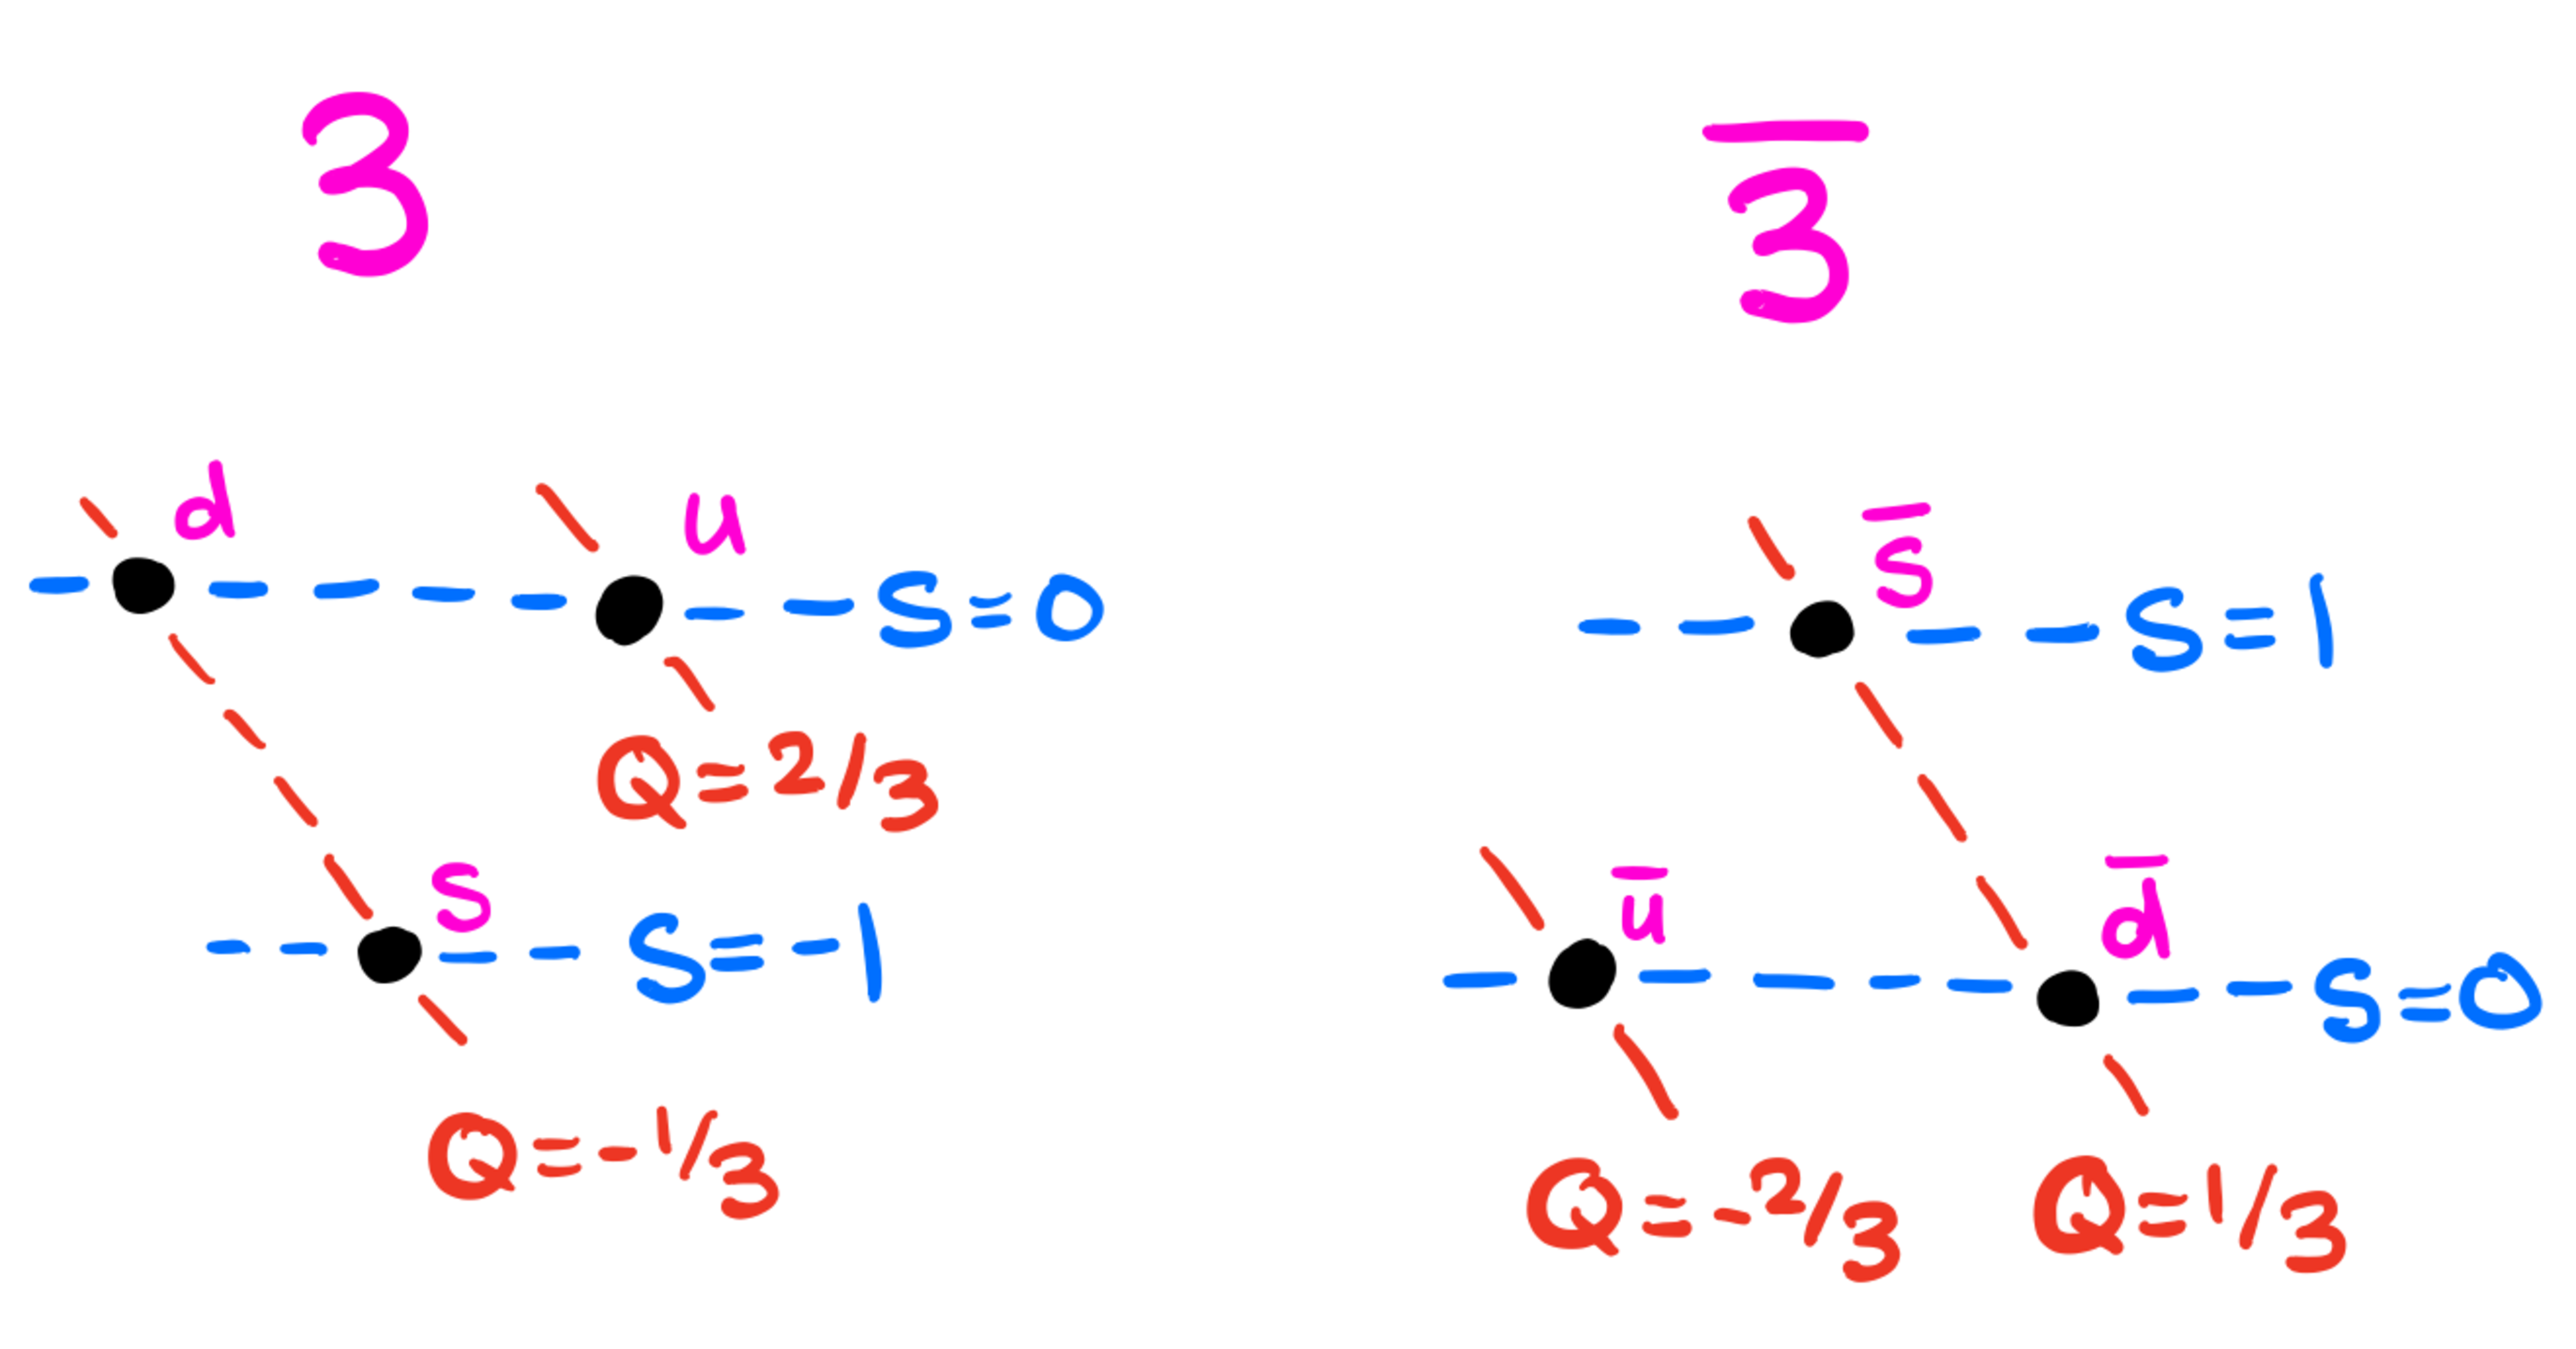
\includegraphics[width = .5\textwidth]{quark_weights}
	\caption{Weight diagram for fundamental and antifundamental of $SU(3)_f$.}
\end{figure}
The octet and singlet states for $s = 0$ (scalar) and $s = 1$ (vector) are shown below. These are obtained by just tensoring together 
the two weight diagrams above.
\begin{figure}[H]
	\centering
	\begin{subfigure}[t]{.38\textwidth}
		\centering
		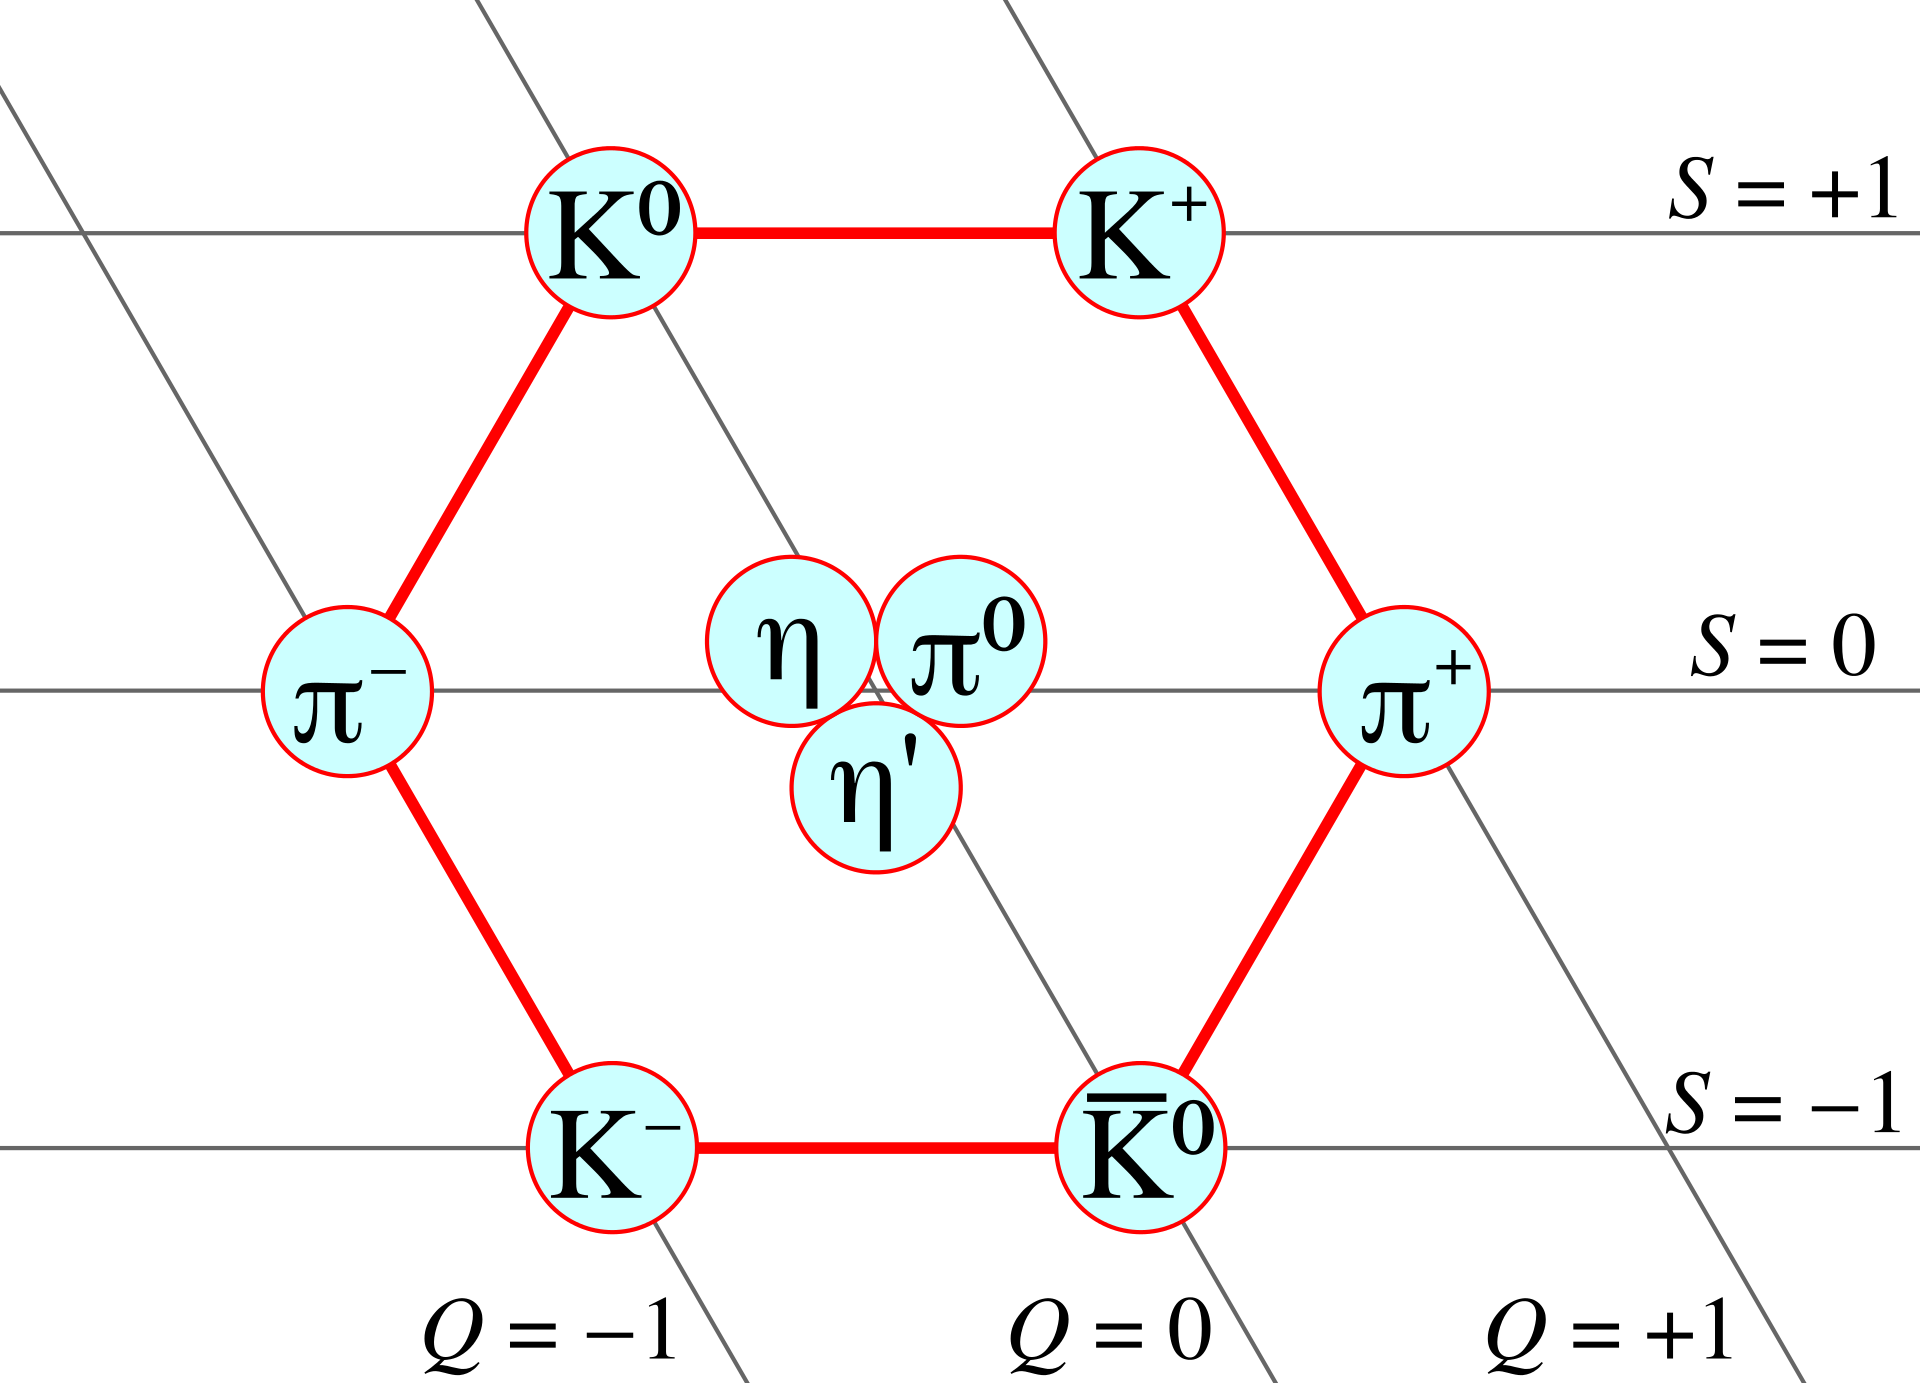
\includegraphics[width = .8\textwidth]{scalar_meson_nonet}
		\caption{Pseudoscalar meson nonet, $J^{PC} = 0^{-+}$.}~
		\label{subfig:scalar_meson_nonet}
	\end{subfigure}
	~
	\begin{subfigure}[t]{.38\textwidth}
		\centering
		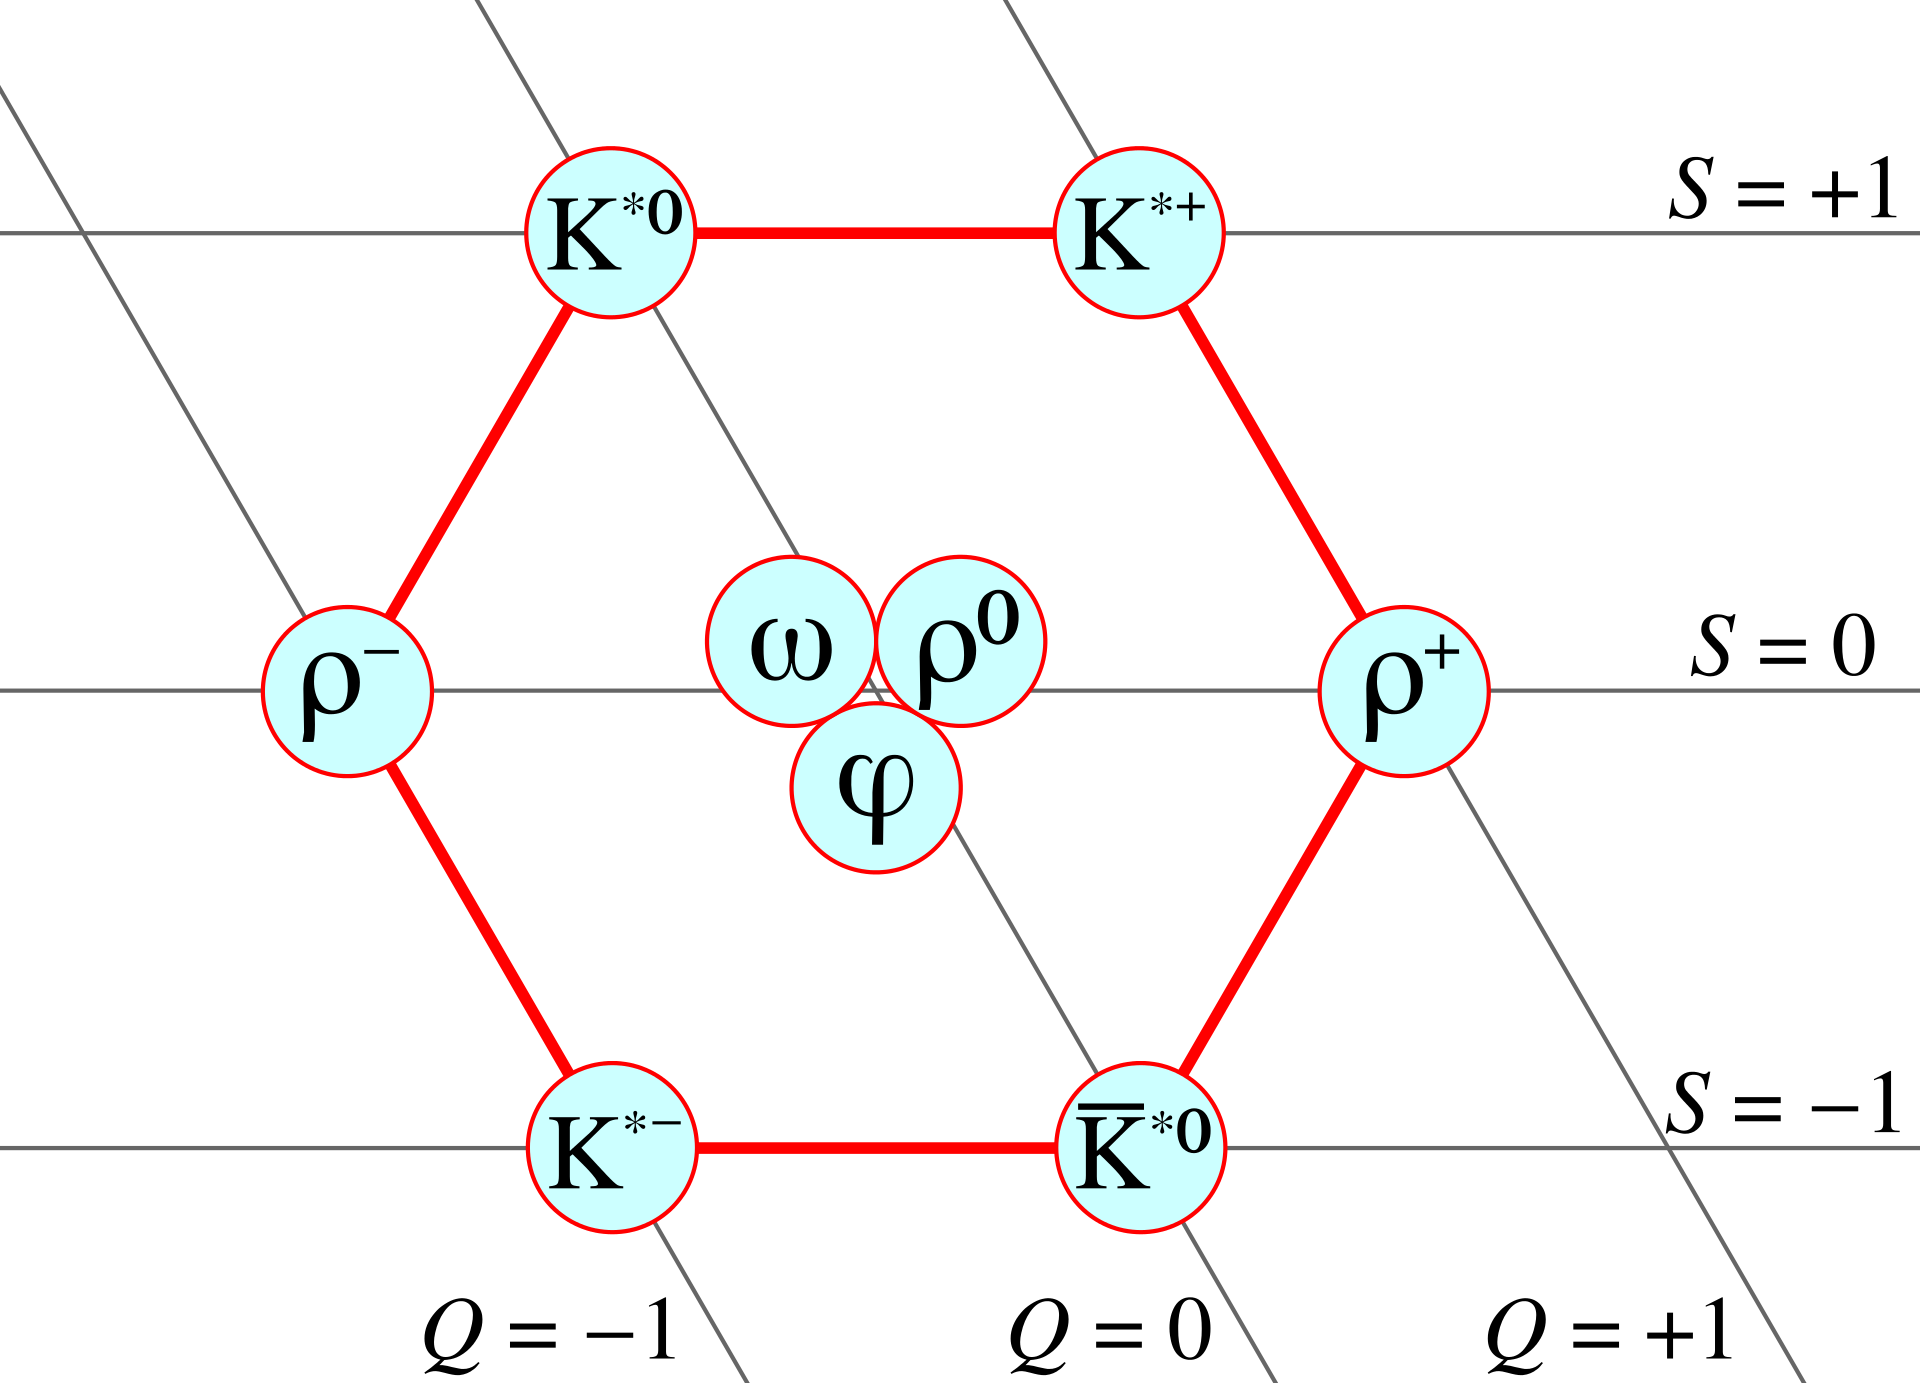
\includegraphics[width = .8\textwidth]{vector_meson_nonet}
		\caption{Pseudovector meson nonet, $J^{PC} = 1^{--}$}~
		\label{subfig:vector_meson_nonet}
	\end{subfigure}
\end{figure}
Each horizontal line has constant strangeness, and each diagonal line has constant charge. The singlet states in each nonet are the 
$\eta$ and the $\phi$ state. 

We can also write these nonets out in terms of their individual fields which transform in the adjoint of 
$SU(3)_f$ (note for the pion multiplet, this gives us the correct transformation law for $\Sigma$ for the vector symmetry $L = R$, 
which is $SU(3)_f$). These presentations of the fields will allow us to also compute their quantum numbers under other 
symmetries, once we have an expression for the symmetry generators. The pseudoscalar nonet fields are packaged into the 
$\mathcal M$ field, and the pseudovector nonet fields into the $\tilde{\mathcal{M}}$ field. 
\begin{align}
	\mathcal M &= \begin{pmatrix} u \\ d \\ s \end{pmatrix} \begin{pmatrix} \overline u & \overline d & \overline s \end{pmatrix} = 
	\frac{1}{\sqrt 2}\begin{pmatrix} \frac{1}{\sqrt 2}\pi^0 + \frac{1}{\sqrt 6} \eta_8 + \frac{1}{\sqrt 6}\eta_0 & \pi^+ & K^+ \\ \pi^- & -\frac{1}{\sqrt 2}\pi^0 + \frac{1}{\sqrt 6} \eta_8 + \frac{1}{\sqrt 6}\eta_0
	& K^0 \\ K^- & \overline K^0 & - \frac{2}{\sqrt 6} \eta_8 + \frac{1}{\sqrt 6}\eta_0 \end{pmatrix} \nonumber \\
	\tilde{\mathcal{M}} &= \frac{1}{\sqrt 2}\begin{pmatrix} \frac{1}{\sqrt 2}\rho^0 + \frac{1}{\sqrt 6}\omega_8 + \frac{1}{\sqrt 6}\omega_0 & \rho^+ & K^{+*} \\ \rho^- & -\frac{1}{\sqrt 2}\rho^0 + \frac{1}{\sqrt 6} \omega^8 + \frac{1}{\sqrt 6}\omega^0
	& K^{0*} \\ K^{-*} & \overline K^{0*} & - \frac{2}{\sqrt 6} \eta_8 + \frac{1}{\sqrt 6}\eta_0 \end{pmatrix}
\end{align}
The notation here is from Burgess and Moore, and is a bit weird: we expect the $\eta$ and $\eta'$ mesons to appear in the pseudoscalar 
nonet, and the $\omega$ and $\phi$ to appear in the pseudovector nonet. These matrices also immediately allow us to read off the quark 
content of each bound state, and along with the weight diagrams it might not hurt to memorize them. We will delve into mass splittings soon, 
and when we do we shall see that the flavor eigenstates in the matrices $\mathcal M$ and $\tilde{\mathcal{M}}$ are not the mass 
eigenstates of the chiral Lagrangian: when isospin symmetry breaks, $m_d - m_u\neq 0$, we must rotate $(\pi^0, \eta_8)$ slightly to form 
the mass eigenbasis. Typically we will instead look at the isospin limit, and in this limit $\eta = \eta_8$ and $\eta' = \eta_0$, and likewise for 
the vector mesons. 

Note also that since the vector mesons are spin 1, the $\tilde{\mathcal{M}}$ field can really have a vector index on it as well, i.e. by 
$\tilde{\mathcal{M}}$ we really mean a field $\tilde{\mathcal{M}}_\mu$, where $\mu$ is a Lorentz index. Each of these mesons are massive 
vector fields, so the $\rho$ is represented by the isospin triplet $(\rho_\mu^\pm, \rho_\mu^0)$ which really contains 12 real scalar fields (with 
9 degrees of freedom for the 3 massive vector fields), etc.

% symmetries for mesons
We wish to write down symmetries of the light quark model for $N_f = 3$ flavors of fermion. These symmetry generators are manifested 
as $3\times 3$ matrices. The first two are known as the \textbf{isospin} $I$ and the \textbf{hypercharge} $y$ (note that $y$ is \textbf{not} the 
Standard Model hypercharge), which are:
\begin{align}
	I = \begin{pmatrix} \frac{1}{2} & 0 & 0 \\ 0 & -\frac{1}{2} & 0 \\ 0 & 0 & 0\end{pmatrix} &&
	y = \begin{pmatrix} \frac{1}{3} & 0 & 0 \\ 0 & \frac{1}{3} & 0 \\ 0 & 0 & -\frac{2}{3} \end{pmatrix} && 
	B = \begin{pmatrix} \frac{1}{3} & 0 & 0 \\ 0 & \frac{1}{3} & 0 \\ 0 & 0 & \frac{1}{3} \end{pmatrix}
\end{align}
$I$ is proportinal to $t^3$, and $y$ is proportional to $t^8$. These are (appropriately normalized) generators of the Cartan subalgebra 
of $SU(3)$, and as such each of our fields we've discussed living in representations of $SU(3)_f$ are charged under each generator. 

The \textbf{electric charge} and \textbf{strangeness charge} are other important quantum numbers, and they are linear combinations 
of $I$, $y$, and $B$:
\begin{align}
	Q = I + \frac{1}{2} y = \begin{pmatrix} \frac{2}{3} & 0 & 0 \\ 0 & -\frac{1}{3} & 0 \\ 0 & 0 & -\frac{1}{3} \end{pmatrix} &&
	S = y - B = \begin{pmatrix} 0 & 0 & 0 \\ 0 & 0 & 0 \\ 0 & 0 & -1 \end{pmatrix}
\end{align}
Conventionally, $S = -1$ for a meson with a strange quark and a different antiquark. The charge of each meson under the symmetry 
generator $X$ can be determined by performing $[\pi^a t^a, X]$ and looking at the eigenvalues of each entry. For example:
\begin{align}
	[\pi^a t^a, Q] = \frac{1}{\sqrt 2} \begin{pmatrix} 0 & \pi^+ & K^+ \\ -\pi^- & 0 & 0 \\ -K^- & 0 & 0 \end{pmatrix} && 
	[\pi^a t^a, I] = \frac{1}{\sqrt 2} \begin{pmatrix} 0 & \pi^+ & \frac{1}{2} K^+ \\ -\pi^- & 0 & \frac{1}{2} K^0 \\ -\frac{1}{2} K^- & -\frac{1}{2} \overline{K}^0 & 0 \end{pmatrix}
\end{align}
We can immediately read off the charged particles from the first commutator. The second set of charges is consistent with how the mesons 
group themselves into isospin multiplets. Since isospin rotates $u\leftrightarrow d$, we expect $(\pi^\pm, \pi^0)$ to be an isospin triplet, 
$K^\pm$ and $(K^0, \overline K^0)$ to be isospin doublets, and $\eta, \eta'$ to be isospin singlets. This is consistent with the doublets 
having charges $I = \pm \frac{1}{2}$ and the triplet having charges $I = 0, \pm 1$. Furthermore, particles in the same isospin multiplet 
will have the same strangeness, since $[I, S] = 0$. The kaons all have the same label despite forming two isospin doublets because the strange quark 
and the strange antiquark have the same mass, so there is no significant mass splitting between the kaons. 

% baryons
To study the spectrum of \textbf{light baryons}, we must consider their spin. For light quarks, baryons are formed from an antisymmetric combination of 
the $q$ field, where $q$ transforms under $SU(3)_f$ in the fundamental as $q = \begin{pmatrix} u & d & s \end{pmatrix}^T$. Baryons are therefore 
states with three identical particles, and must obey symmetry properties based on their spin. Baryons are evidently fermions since they are 
formed from an odd number of spin $\frac{1}{2}$ particles, and thus must obey Fermi statistics and be antisymmetric under interchange of 
particles. Note that mesons don't need to satisfy this because $q$ and $\overline q$ are distinguishable. 

The baryon wavefunction is defined by:
\begin{align}
	|\mathcal B\rangle = \sum_{\sigma_1 \sigma_2\sigma_3} \sum_{r_1 r_2 r_3} \sum_{f_1 f_2 f_3} \int_{p_1 p_2 p_3} \psi\left(\{p_i, \sigma_i, r_i, f_i\}\right) 
	a_1^\dagger a_2^\dagger a_3^\dagger |G\rangle \\
	\psi = (\textnormal{spin})(\textnormal{color})(\textnormal{flavor})(\textnormal{space}) = \textnormal{antisymmetric}
\end{align}
where $\sigma$ is a spin label, $r$ is a color label, $f$ is a flavor label, and $p$ is a momentum. Since baryons are color singlets and proportional to 
$\epsilon^{rst} q_r q_s q_t$, the color portion of the baryon wavefunction must be antisymmetric, and therefore the rest of the wavefunction must be 
be symmetric. In its ground state, the angular momentum of the baryon is $\ell = 0$, which means that the spatial part of the wavefunction is symmetric 
under interchange with $(-)^\ell = +$, hence we can factor off this piece as well. This means that \textbf{for a ground state baryon, the product of its flavor 
and spin degrees of freedom must be symmetric} for the baryon to be a fermion, which allows us to constrain the spectrum. 

The possible spin and flavor states a baryon can take on are given by the following representations of $SU(2)$ and $SU(3)_f$, respectively:
\begin{align}
	\bf \frac{1}{2}\otimes \frac{1}{2}\otimes \frac{1}{2} = \frac{1}{2}\otimes\frac{1}{2}\otimes\frac{3}{2} && 
	\bf 3\otimes 3\otimes 3 = 1 \oplus 8\oplus 8\oplus 10
\end{align}
The different $\bf \frac{1}{2}$ and $\bf{8}$ multiplets all have mixed symmetry properties and the $\frac{3}{2}$ and $\bf 10$ multiplets are completely symmetric irreps. 
Thus there are two ways to form a symmetric flavor-spin wavefunction: combining the symmetric irreps as a product, and taking appropriate combinations 
of the mixed symmetry irreps. The symmetric $\bf 10$ irrep is known as the \textbf{baryon decuplet}, which is spin $\frac{3}{2}$ and therefore has 40 states. 
Only eight flavor states survive from the two octets when symmetry is considered, and therefore we are left with a single \textbf{baryon octet} which is 
spin $\frac{1}{2}$, contributing 16 baryon states. There are thus $56$ linearly independent baryon states one can construct from the light quarks. The weight 
diagrams for the octet and decuplet are shown below with the corresponding baryon states named.
\begin{figure}[H]
	\centering
	\begin{subfigure}[t]{.38\textwidth}
		\centering
		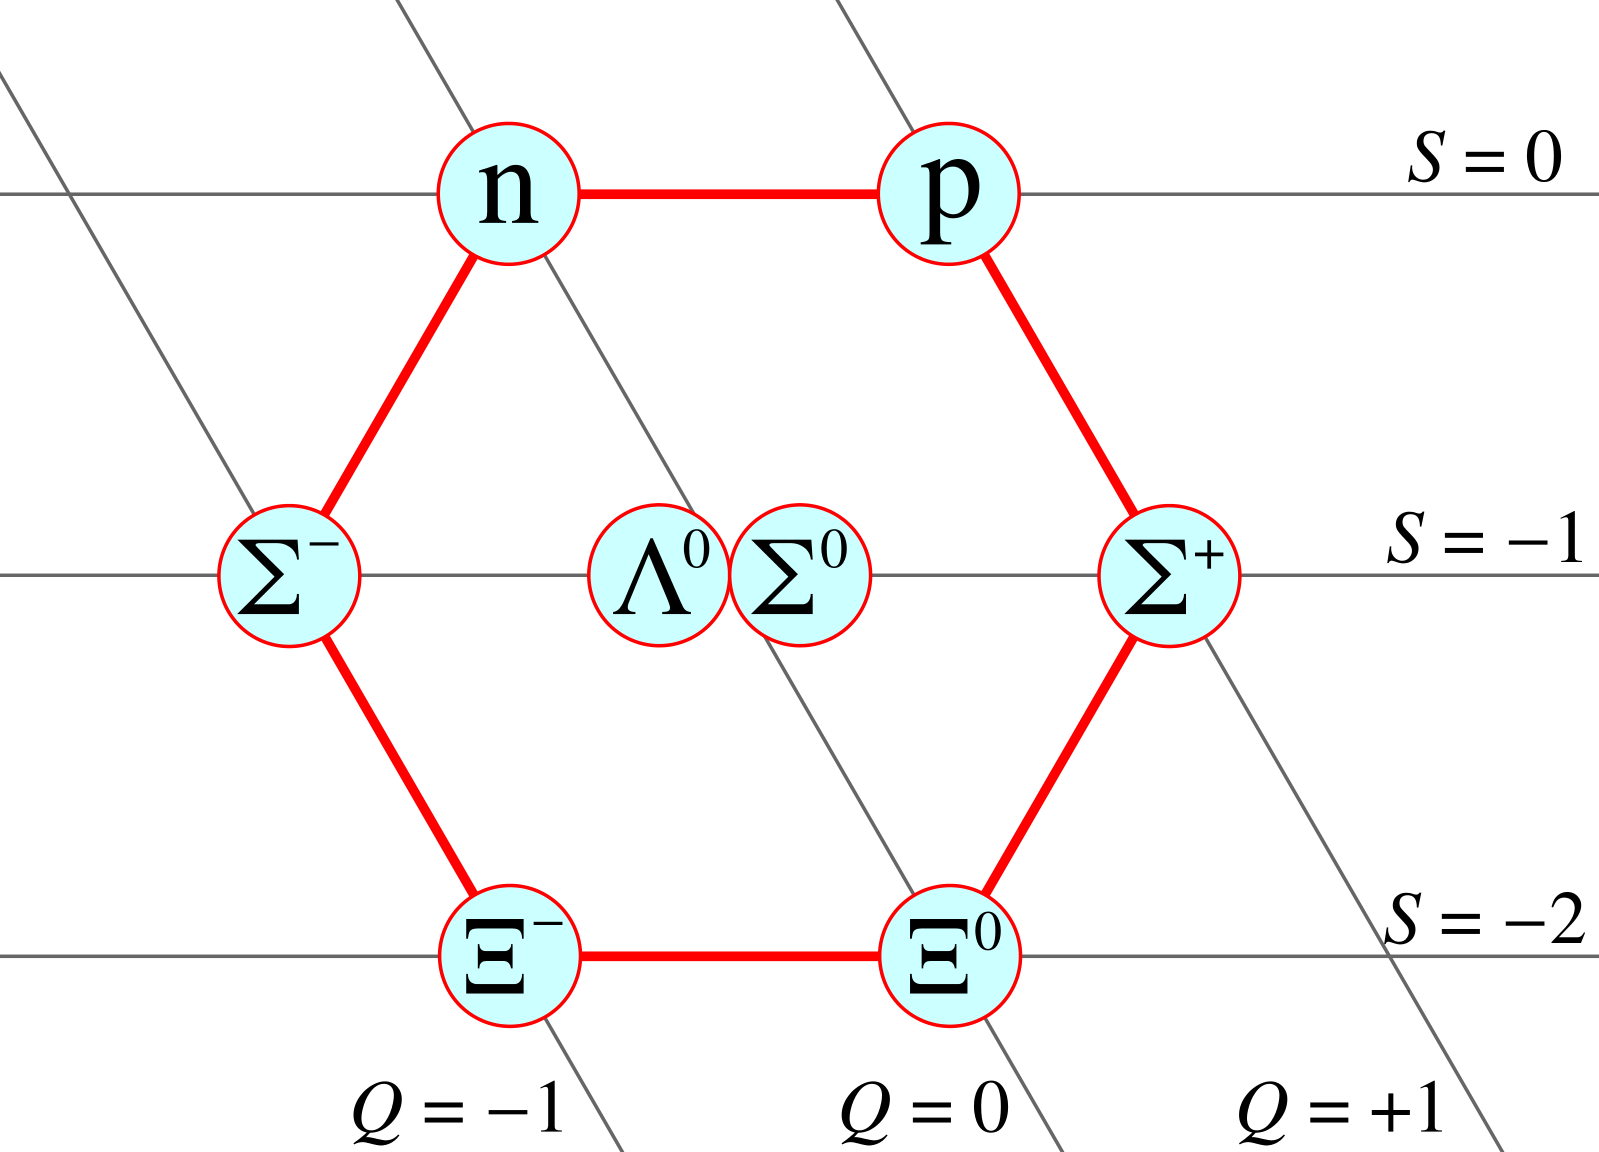
\includegraphics[width = .8\textwidth]{baryon_octet}
		\caption{Spin $\frac{1}{2}$ baryon octet.}~
		\label{subfig:baryon_octet}
	\end{subfigure}
	~
	\begin{subfigure}[t]{.38\textwidth}
		\centering
		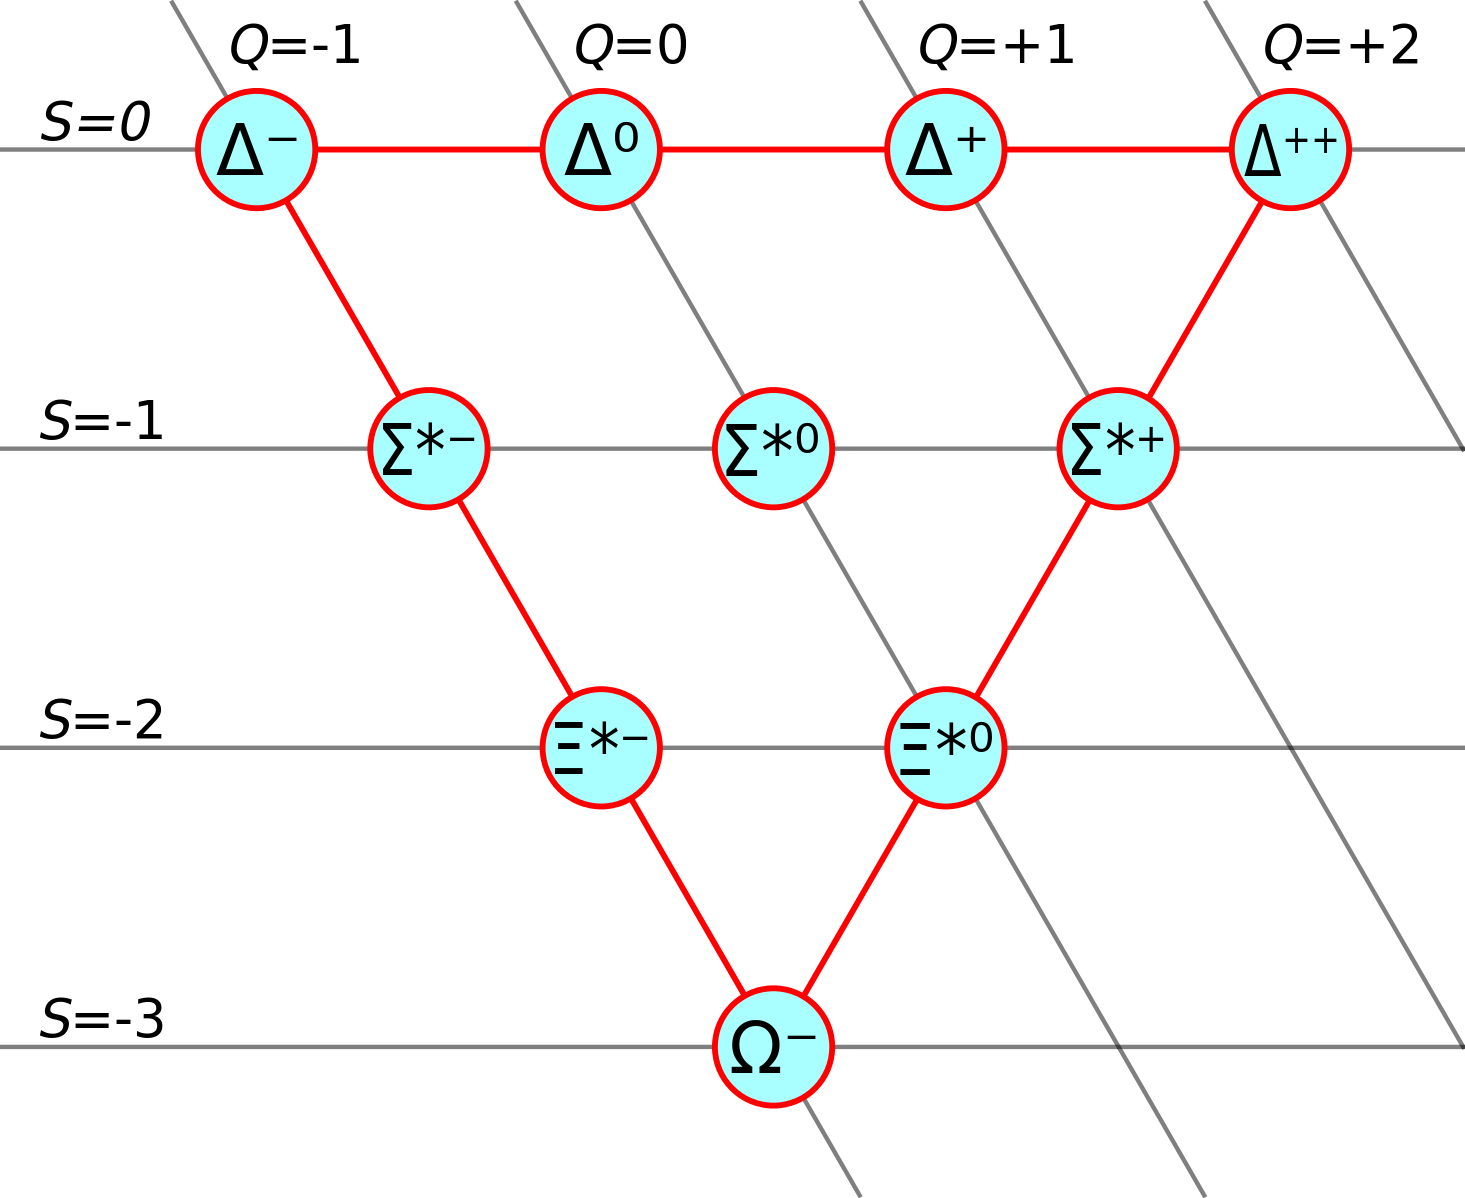
\includegraphics[width = .8\textwidth]{baryon_decuplet}
		\caption{Spin $\frac{3}{2}$ baryon decuplet}~
		\label{subfig:baryon_decuplet}
	\end{subfigure}
\end{figure}

It is useful to write the bound states in the octet as a matrix of fields which transforms in the adjoint of $SU(3)_f$, much like the matrices 
$\mathcal M$ and $\tilde{\mathcal{M}}$. This allows us to read off the quark content of each field easily and compute its quantum numbers. 
The subtlety here is that a baryon in the octet is made of 3 quarks, two of which are antisymmetrized. Since $\bf 3\otimes 3 = 6\oplus\overline 3$ with 
$\overline 3$ the antisymmetric combination $\epsilon^{ijk}q_j q_k$, we see that this antisymmetric combination of quarks transforms just like $\overline q^i$. 
Hence to write out the baryon matrix, we can take an outer product of $q^i$ with $\epsilon^{ijk} q_j q_k\sim\pm [q_j, q_k]$, where $[\cdot, \cdot]$ is the 
commutator of fields. We will call the matrix which represents this combination of fields by $\mathcal B$:
\begin{equation}
	\mathcal B = \begin{pmatrix} u \\ d \\ s \end{pmatrix} \begin{pmatrix} [d, s] & [s, u] & [u, d] \end{pmatrix} = 
	\begin{pmatrix} \Sigma^0 + \frac{1}{\sqrt 3}\Lambda_8 & \Sigma^+ & p^+ \\ \Sigma^- & -\Sigma^0 + \frac{1}{\sqrt 3}\Lambda_8 & n^0 \\ \Xi^- & \Xi^0 & -\frac{2}{\sqrt 3}\Lambda_8
	\end{pmatrix}
\end{equation}
Here $p^+$ is the proton field and $n^0$ is the neutron field. This is just like the two meson octets, except the quark content is different and a bit 
more complicated because each $\overline q$ is replaced with a commutator of the other quarks. It is also a bit easier to tell the isospin multiplets 
apart in this case; in the meson case, the kaons split into two different isospin doublets, but here it is obvious that $(p^+, n^0)$ and $(\Xi^-, \Xi^0)$ split 
into different isospin doublets. 

One can also see that in the baryon decuplet, some of the particles just look like excited states of the $\Sigma$ and the $\Xi$ baryons. 
The $\Delta^+$ and $\Delta^0$ baryons can also be looked at as excitations of the proton and neutron since they have the same quark 
contents, although they fall into a larger isospin multiplet with $\Delta^++$ and $\Delta^-$. 

\subsection{Mass relations}

Before we get into quantitative predictions for hadron masses, let's briefly sketch out some heuristic arguments about what we expect to see from the observed mass spectrum. 
Since isospin is \textit{almost} a good symmetry, we expect \textit{the particles in an isospin multiplet to have nearly degenerate masses} (for example, 
the $(\pi^\pm, \pi^0)$ isospin triplet or the two isospin doublets $(K^+, K^0)$ and $(K^-, \overline K^0)$. Note that the kaons live in distinguished isospin 
doublets can be seen because each doublet has a different strangeness charge. This near degeneracy is confirmed in experiments. If we let $\Lambda_c$ 
be the approximate energy of a QCD bound state, we can see that $\Lambda_c\approx 500\;\mathrm{MeV} - 1\;\mathrm{GeV}$. Since the different isospin 
multiplets differ in their strangeness quantum number, we expect the mass splittings between each multiplet to be about $m_s / \Lambda_c\approx 
20\%$ to $25\%$, and this is confirmed in experiments. This applies to both baryons and mesons (other than the pions, which have no strangeness), and we'll 
thus \textit{typically see the isospin multiplets in each $SU(3)_f$ multiplet split by about 150 - 200 MeV}. 

Now, onto mesons. We've already studied some mass relations with the chiral Lagrangian, but here we will go into a little more depth and also examine some mixing that we 
may have glossed over previously. We previously saw by expanding out the fields in the 2-flavor chiral Lagrangian using the mass term
\begin{equation}
	\mathcal L_\chi\supset \frac{\mu}{2}\;\mathrm{tr}\left[M_q (\Sigma + \Sigma^\dagger)\right]
\end{equation}
that we had the Gell-Mann Oakes Renner relation linearly relating $m_\pi^2$ to $m_u + m_d$, and that we could perform a similar 
computation in $N_f = 3$ flavor $\chi$PT to derive the Gell-Mann Okubo relation between $m_K^2$, $m_\eta^2$, and 
$m_\pi^2$. This did not tell the full story: namely, there is also mixing between some of these states when we are not working in 
the isospin limit, and we get terms proportional to $(m_d - m_u) \pi^0 \eta_8$ which mean the naive $\pi^0$ and $\eta_8$ we used 
in the field $\pi^a t^a$ are not mass eigenstates. Expanding out the mass term in $\mathcal L_\chi$ gives the following coupling which mixes the 
$\pi^0$ and $\eta_8$ flavor eigenstates:
\begin{equation}
	\mathcal L_\chi\supset -\frac{1}{2}\mu\begin{pmatrix} \pi^0 & \eta_8 \end{pmatrix} \begin{pmatrix} \frac{1}{2} (m_u + m_d) & \frac{1}{2\sqrt 3} (m_u - m_d) \\ 
	\frac{1}{2\sqrt 3} (m_u - m_d) & \frac{1}{6} (m_u + m_d + 4 m_s) \end{pmatrix} \begin{pmatrix} \pi^0 \\ \eta_8 \end{pmatrix}
\end{equation}
This matrix must be diagonalized to find the meson states with definite mass. Since it is symmetric it can be diagonalized with a rotation in $SO(2)$, and we 
let $\pi^0_m$ and $\eta$ be the new eigenstates:
\begin{equation}
	\begin{pmatrix} \pi^0_m \\ \eta \end{pmatrix}  = \begin{pmatrix}\cos\theta & \sin\theta \\ -\sin\theta & \cos\theta \end{pmatrix} \begin{pmatrix} \pi^0 \\ \eta_8 \end{pmatrix}
\end{equation}
This mixing angle $\theta$ can be shown using mass relations to directly measure the amount of isospin breaking:
\begin{equation}
	\tan 2\theta \approx\frac{\sqrt 3}{2} \left( \frac{m_d - m_u}{m_s} \right)
\end{equation}
hence $\theta$ is very small and its effects can be neglected for the most part. The real $\pi^0$ that we work with is really the $\pi^0_m$ particle after 
mixing of flavor eigenstates, but the effects of the mixing are almost negligible. The $\eta_0$ cannot mix with either the $\pi^0$ or the $\eta$ particle because 
it lives in a different multiplet of $SU(3)_f$: one would think that it could potentially mix to a very small amount because $SU(3)_f$ is an approximate symmetry, 
but it can be shown that there is actually no mixing. This means the $\eta'$ lives solely in the $SU(3)_f$ singlet, while the $\pi^0$ and $\eta$ live entirely in the 
$SU(3)_f$ pseudoscalar octet.

However, in the vector nonet the story is a little different. Here, the particles that can potentially mix with one another are the $\rho^0$, the $\omega_8$, and the 
$\omega_0$. Any mixing of the $\rho^0$ will violate isospin, so while this will happen to some degree, as with the $\pi^0$ mixings into $\eta$ and $\eta'$, we 
will ignore it and assume it is negligible. The interesting story appears when we talk about $\omega_0$ and $\omega_8$ mixing, which happen to be strongly mixed. 
Their mass eigenstates are denoted by the $\omega$ and the $\phi$. The quark content of these two flavor states is:
\begin{align}
	\omega_8\sim \frac{1}{\sqrt 3} (u\overline u + d\overline d - 2s\overline s) && \omega_0\sim \frac{1}{\sqrt 3} (u\overline u + d\overline d + s\overline s)
\end{align}
and their mass eigenstates end up having quark content:
\begin{align}
	\omega\sim \frac{1}{\sqrt 2} (u\overline u + d\overline d) && \phi\sim s\overline s
\end{align}
Note that $\omega_0$ and $\omega_8$ are isospin singlets, while $\rho^0$ is in an isospin triplet. Since isospin is technically only approximately 
conserved, there may be some very small mixing effects from $\rho^0$ into the other two mesons; however, since it is very close to being a good 
symmetry, we don't really need to worry about this small amount of mixing, and we can assume the $\rho^0$ doesn't really mix into the 
other states. 
% https://physics.stackexchange.com/questions/432102/rho-and-omega-meson-mixing

% baryon masses
Let us move to the baryon masses: we can begin by estimating how the masses of each of the two irreps should compare. The flavor decuplet is totally symmetric in the spins 
and the octet has mixed symmetry, so the hyperfine effects between the quarks which go as $\langle \vec S_i\cdot\vec S_j\rangle$ will add their 
interaction energy to the mass of the decuplet states, while the hyperfine effects will be negative for certain quark pairs in the octet. Thus we expect 
the decuplet states to begin at a slightly higher baseline mass than the octet states. That is exactly what we see in nature; the octet states include the 
lightest baryons, the $p^+$ and $n^0$, and the heaviest light baryon is the $\Omega^- \sim sss$, which is in the decuplet. 

We can qualitatively approach this problem for the baryon octet. Under a vector transformation $V\in SU(3)_f$, we designed the baryon octet matrix $\mathcal B$ 
to transform as $\mathcal B\rightarrow V \mathcal B V^\dagger$. So, to describe the low energy dynamics of baryons, we must determine an effective Lagrangian for 
the $\mathcal B$ field which is invariant under this approximate $SU(3)_f$ symmetry. Note that in the limit of $SU(3)_f$ symmetry, each particle in the multiplet would have the 
same mass; to study how their masses differ, we therefore need to study how the explicit symmetry breaking of $SU(3)_f$ affects the baryon octet. We will thus derive relations 
between the masses of different fields in the baryon octet, but we will need a baseline measurement to know what the absolute mass scales are.

\begin{answer}
\textbf{Proton-neutron mass splitting} 

\begin{flushleft} \setlength{\parindent}{2em}
	The proton-neutron mass difference is a very simple thing to compute roughly-- in the isospin limit, the only difference in the proton and neutron 
	masses will be the electromagnetic contribution to their energies, since $p^+$ is charged and $n^0$ is not. In this limit, we can model the extra 
	energy the proton gains by a Coulomb potential with radius $r = r_P\approx 1 \;\mathrm{fm}$. This gives us:
	\begin{equation}
		\Delta E_\mathrm{EM}\approx \frac{e^2}{4\pi r} \approx \frac{\alpha}{1\;\mathrm{fm}}(200\;\mathrm{MeV}\times\mathrm{fm})\approx 1 \;\mathrm{MeV}
	\end{equation}
	where we use $\Lambda_\mathrm{QCD}\approx 1\;\mathrm{fm}^{-1}\approx 200\;\mathrm{MeV}$. This quite neatly gives the approximate 
	mass splitting between the $p^+$ and the $n^0$!
\end{flushleft}
\end{answer}

\subsection{Light meson decays}

Typically when we compute light meson decays, we don't resort to the parton model but instead acknowledge our ignorance about 
full non-perturbative QCD with structure functions or decay constants. We saw this in the decay of the charged pion: instead of 
computing a full partonic process, which would involve diagrams at the quark level, we parameterized the axial matrix element $\langle 
0 | j_5^{\mu a} | \pi^b\rangle$ with the pion decay constant $f_\pi$. 

When thinking about light hadron decays, it's often useful to think of what would happen if certain sectors were turned off. At high energies, 
the strong force is perturbative and we can therefore use perturbation theory to get estimates on decay rates of massive hadrons, with mass 
scales $m >> \Lambda_\mathrm{QCD}$. However, at lower mass scales we can still get some information about decay rates from perturbation 
theory. Consider decays in the pseudoscalar octet when the weak force is turned off. The weak force is the only one which provides flavor 
changing currents, and since each particle in the octet is the lightest hadron with its quark composition, \textit{the pseudoscalar octet 
is stable in the presence of just the strong and electromagnetic forces}. This implies that any decay occurring in the pseudoscalar octet 
will be able to be thought of perturbatively, since the decay is through the weak force, which is perturbative. There are still non-perturbative 
bits which contribute and are encoded in the meson decay constants, but the quark diagrams should give estimates of decay rates. 

Usually in these decays one can use $\Lambda_\mathrm{QCD}$ as a rough mass scale if you try to compute things from the ground up with 
quark diagrams. For example, in the hadronic decay $K^-\rightarrow\pi^0\pi^-$. This decay occurs at the quark level through the $s$ quark 
emitting a $W^- u$ and the $W^-$ decaying into $d\overline u = \pi^-$, and so we can approximate the decay rate as:
\begin{equation}
	\mathcal M(K^-\rightarrow\pi^-\pi^0)\approx V_{us} V_{ud} G_F (\mathrm{kinematics})\implies \overline{|\mathcal M|^2}\approx \lambda^2 G_F^2 \Lambda^6
\end{equation}
Integrating this over phase space and using the relevant scale of $\Lambda_\mathrm{QCD}$, we find a decay width for two final state particles 
of approximately:
\begin{equation}
	\Gamma(K^-\rightarrow\pi^-\pi^0)\approx \frac{1}{2\Lambda_\mathrm{QCD}}(2\pi)^4\frac{1}{(2\pi)^6}(2\pi)\frac{1}{2^2}\overline{|\mathcal M|^2} = \frac{1}{16\pi}\lambda^2 G_F^2 
	\Lambda_\mathrm{QCD}^5
\end{equation}
Plugging in $\lambda\approx 0.22$, $G_F \approx 10^{-5} \;\mathrm{GeV}^{-2}$, and $\Lambda_\mathrm{QCD}\approx 0.2\;\mathrm{GeV}$, we get 
$\Gamma\approx 100 \;(\mu s)^{-1}$ for the decay and a lifetime of about $\tau\approx 10^{-2} \;\mu s$, which is close to the width provided by the PDG.
We'll see how to do this decay properly and take into account all the non-perturbative physics with form factors, after a simpler example to show 
the utility of decay constants being used in more general pseudoscalar decays.

We can parameterize the rest of the axial currents as well, including pseudoscalar mesons which do not arise strictly from chiral 
symmetry breaking, like the $D^+$ or the $B^+$. Let $P\in \{\pi^\pm, K^\pm, D^\pm, D_s^\pm, B^\pm\}$ be a pseudoscalar meson 
made of quarks $q_1$ and $\overline q_2$. Then the \textbf{pseudoscalar meson decay constant} $f_P$ is defined by parameterizing 
the axial current which connects $P$ with the vacuum:
\begin{equation}
	\langle 0 | \overline q_1 \gamma^\mu \gamma_5 q_2 | P(p)\rangle = i f_P p^\mu e^{-ip\cdot x}
\end{equation}
This is the generalization of the matrix element which defines the pion as a Goldstone boson. The decay constant $f_P$ must be measured 
through experiment or on the lattice, just like how the pion decay constant is measured through matching experimental results to 
the width $\Gamma(\pi^+\rightarrow\mu^+ \nu_\mu)$; \textbf{$f_P$ is typically around the scale of $\Lambda_\mathrm{QCD}$}. 

Using this parameterization, one can determine the decay width at first order in perturbation theory. The pseudoscalar meson interacts with the 
axial current $\overline q_1\gamma^\mu\gamma_5 q_2 = j_5^{\mu a}$ for some $a$, and this axial current couples to the leptonic currents 
$\overline\ell \gamma^\mu P_L \nu_\ell$ with a coupling of $G_F V_{12}$, where $V_{12}$ is the CKM matrix element connecting the quark 
pieces. Combining the decay constant from the current insertion and the weak coupling gives us about the same answer as in $\pi^+\rightarrow 
\mu^+\nu_\mu$, with an additional factor for the CKM matrix:
\begin{equation}
	\Gamma(P^+\rightarrow\ell^+\overline\nu_\ell) = \frac{1}{4\pi} |V_{q_1 q_2}|^2 G_F^2 f_P^2 m_P m_\ell^2 \left(1 - \frac{m_\ell^2}{m_P^2}\right)^2
\end{equation}

Fully computing hadronic light decays is harder, because it involves a more complicated parameterization for the matrix elements. Although we 
can usually approximate it with a quark diagram using $\Lambda_\mathrm{QCD}$ as our mass scale, to fully work out the computation we need 
to use form factors. For example, consider the $K^+\rightarrow\pi^+ \pi^0$ decay. The interaction describing hadronic weak decays is fully 
contained in the weak interaction Lagrangian:
\begin{equation}
	\mathcal L_\mathrm{q, weak} = \frac{4 G_F}{\sqrt 2} V_{ij} V_{lk}^* [\overline u_i \gamma^\mu P_L d_j] [\overline d_k \gamma_\mu P_L u_l] + h.c.
\end{equation}
This amounts to the computation of the matrix element $\langle\pi^+\pi^0 | \mathcal L_\mathrm{weak} | K^+\rangle$, which means we need to select 
the appropriate pieces of the interaction current. By the quark diagram which connects $K^+$ to $\pi^+ \pi^0$, we can read off the correct pieces: 
we'll need an interaction that flips the initial $\overline s$ in $K^+$ into a $\overline u$, and one which turns the emitted $W^+$ into a $u$ and $\overline d$; 
thus we need $V_{us}$ and $V_{ud}^*$, and need to compute the matrix element:
\begin{equation}
	\langle\pi^+\pi^0 | (\overline u \gamma^\mu P_L s)(\overline d\gamma_\mu P_L u) | K^+\rangle
\end{equation}
The idea here is that both currents are elements of $j_L^{\mu a}$ for specific values of $a$, so each current transforms in the octet $\bf 8$ of 
$SU(3)_f$; here we have $c = 4$ for the first one, and $d = 1$ for the second one. The pions and kaon likewise transform in the pseudoscalar 
octet, so they also have an $a$ index ranging from 1 to 8. The matrix element can then be parameterized as the most general 5-index tensor $X^{abcde}$ 
with $c = 4$ and $d = 1$ which can be made up of the invariant symbols of $SU(3)_f$, which are $\delta_{ab}$, $f_{abc}$, and $d_{abc}$. 
Writing out all possible combinations of these gives Eq.~(9.98) of Burgess and Moore, which is an expansion of this matrix element in form 
factors. At the end setting $c = 4$, $d = 1$, $a, b\in\{1, 2, 3\}$ for pions, and $e\in \{4, 5, 6, 7\}$ for charged pions yields 3 form factors that 
the final matrix element can be written in terms of.

I mostly included the last paragraph for completeness; I highly doubt that we'll need to compute parameterizations like this on the exam. However, 
it's good to know how these decays are actually computed: use symmetry properties to determine what irreps certain currents transform in, then 
write the most general expansion with these indices that you can, and take the correct components to reduce the relations that you have. 
Instead, a rougher way to do this is to compute the quark diagram and plug in values of $\Lambda_\mathrm{QCD}$ as appropriate: you should 
get an answer which is roughly correct. 

% TODO if time: \Delta I = 1/2 rule.

\subsection{Meson mixing}

Meson mixing is a pretty complicated subject, so I'm only going to brush the surface. 
We need to look at neutral systems to study mixing, because if two particles have similar quark content or other 
properties but different charges under some symmetry group, then they will not be able to mix. This is why the candidates for flavor$\leftrightarrow$mass 
mixing are typically neutrinos and neutral mesons. Here we'll study kaons, but one can redo this exact same analysis with $B$ mesons. 
{\color{red} TODO why not D mesons?}

Let's take a look at the neutral kaons, $K^0 = d\overline s$ and $\overline K^0 = s\overline d$. 
Charge conjugation has $C|K^0\rangle = |\overline K^0\rangle$ and similarly for $|\overline K^0\rangle$. Since these mesons are 
pseudoscalars, we see that $CP|K^0\rangle = - |\overline K^0\rangle$ and vice versa\footnote{Note that Schwartz seems to think that $CP|K^0\rangle 
= |\overline K^0\rangle$ and vice versa, which makes the definition of the CP eigenstates opposite. He may just be switching conventions 
on the global phase for parity, and it shouldn't really matter except for the relative sign in the definitions of $|K_\pm\rangle$. The 
rest of the story is the same, just be consistent with how you define $|K_\pm\rangle$ and nothing else will change.}. 
This means that we can form eigenstates of $CP$, denoted by their eigenvalue:
\begin{equation}
	|K_\pm\rangle := \frac{1}{\sqrt 2}\left( |K^0\rangle\mp |\overline K^0\rangle\right)
\end{equation}
Note that $|K_\pm\rangle$ refers to the CP eigenstates of the neutral $K^0, \overline K^0$ system, while $|K^\pm\rangle$ refers to the charged kaons. 
% My CP convention is here: http://www.personal.soton.ac.uk/ab1u06/teaching/phys3002/course/20_PCCP.pdf

One can now undertake an extensive analysis of how these eigenstates differ from the mass eigenstates which the neutral kaons propagate in. 
If the weak interactions didn't violate CP 
(since the Jarlskog invariant is nonzero), then CP would be a good quantum number for the theory and the energy (mass) eigenstates would 
have definite CP. However, there is a small but nonzero amount of CP violation in the weak sector of the SM, which we discussed previously. 
This small violation of CP means that the mass eigenstates of the neutral kaon system are closely related to the CP eigenstates, but there is a 
small amount of interference between the terms.
The mass eigenstates are called \textbf{K-long} and \textbf{K-short}, after their lifetimes, and they are defined as:
\begin{align}
	|K_L\rangle := |K_+\rangle + \epsilon |K_-\rangle && |K_S\rangle := |K_-\rangle - \epsilon |K_+\rangle
\end{align}
Here $|\epsilon|\approx 10^{-3}$ gives a rough estimate of CP violation.

The $K_L$ particle takes a much longer time to decay than the $K_S$ particle, which is because each of these 
particles is very close to being a CP eigenstate. This is easy to see from the definitions. Neutral kaons decay via 
the weak force (because flavor is conserved by the other two forces, and the kaons are the lightest particles with their respective 
quark flavors), into a charged pion and a $W^\pm$. The $W$ further decays into either a pion or a lepton-neutrino pair. 

Let's look at how the CP eigenstates decay to pions to determine which one decays faster. An neutral $n$-pion state will have 
CP eigenvalue $CP|n\pi\rangle = (-)^n (-)^\ell |n\pi\rangle$ because each pion is odd under $CP$, and we can add parity by 
splitting off a factor of $(-)^\ell$. In the ground state $\ell = 0$, so the n-pion states have $CP = (-)^n$. The lowest number 
of pions in a CP even state is 2, and the lowest number in a CP odd state is 3; hence we can assume that the 
even CP kaon state $|K_+\rangle$ will (mostly) decay to 2 pions, and the odd CP kaon state $|K_-\rangle$ will decay to 3 pions. 
The key observation here is that $3 m_\pi\approx 420\;\mathrm{MeV}$, while $2 m_\pi\approx 280\;\mathrm{MeV}$; the energy 
difference in these decays compared to the kaon mass of $\approx 490\;\mathrm{MeV}$ is significant. The 2 pion decay channel will 
thus be significantly more favored, and so the CP even eigenstate will decay faster. This means that $K_S$ will be in a superposition 
with predominantly the $K_+$ eigenstate, while $K_L$ will be in a superposition with mostly the $K_-$ eigenstate. 

At this point we can confirm this with the PDG: the $K_S$ particle will decay primarily into two pions ($K_S\rightarrow 2\pi^0$ and $K_S\rightarrow 
\pi^+\pi^-$ have a combined BR of about 99\%), while the $K_L$ particle will decay into 3 pions about 33\% of the time, and decay semileptonically 
the rest of the time. The kaons lifetimes are approximately:
\begin{align}
	\Gamma(K_L)\approx 5\times 10^{-8} && \Gamma(K_S)\approx 9\times 10^{-11}
\end{align}
so one can see this computation manifested in the data. Furthermore, \textit{measurements of $K_L$ decay to two pions, 
$K_L\rightarrow\pi^+\pi^-$, can be used to test CP violation in the Standard Model}, since this decay can only occur from 
the $K_+\rightarrow\pi^+\pi^-$ decay which is contained in $K_L$ with a factor of the CP violating parameter $\epsilon$. 
In fact, \textbf{the existence and measurement of the process $K_L\rightarrow 2\pi$ was what first led physicists to conclude that 
there was CP violation in the Standard Model}. 

There are two types of CP violations which may occur in the decay of $K_L\rightarrow 2\pi$. The first is what we have already discussed; 
\textbf{indirect CP violation} refers to CP violation in which $K_L$ has a small component $\epsilon K_+$ which can decay to $2\pi$. The 
other type of CP violation which can contribute to this decay is called \textbf{direct CP violation}, and it is present because \textit{when CP is violated, 
$K_-$ can decay directly to $2\pi$}. The parameter measuring direct CP violation is called $\epsilon'$, and it has been measured to be 
even smaller than $\epsilon$, so there is not much direct CP violation going on. Note that indirect CP violation occurs because the CP eigenstates 
mix together to form a mass eigenstate, and direct CP violation occurs because CP is not conserved in the weak interactions. 

The difference between the flavor eigenstates $K^0$ and $\overline K^0$ and the mass eigenstates $K_L$ and $K_S$ leads to flavor oscillations. 
If we have a beam of $K^0$ particles prepared, we can measure how often they will oscillate into $\overline K^0$ thanks to propagation in the 
form of $K_L$ or $K_S$. The frequency of this oscillation $\Omega$ is about equal to $\Delta m = m_{K_L} - m_{K_S}$, as seen in the 
formulas in Burgess and Moore:
\begin{align}
	P_{K^0\rightarrow K^0}(t)\approx A(1 + B \cos(\Delta m t)) && P_{K^0\rightarrow \overline K^0}(t)\approx A'(1 - B \cos(\Delta m t))
\end{align}

\subsection{Heavy quark spectrum}

When we discuss heavy quarks, we're usually talking about hadrons with a $c$, $b$, or $t$ quark. We won't talk about top quarks here at 
all because we've already seen that the top quark doesn't hadronize, as it decays to $b W^+$ faster than the time it takes to hadronize. 
We'll start with the $D$ and $B$ mesons, which contain one $c$ or $b$ quark and one other quark. 

As the $c$ and $b$ are heavy quarks, their meson masses are a bit easier to reason out. The $c$ mass is about $1.3$ GeV and the 
$b$ mass is about $4.7$ GeV; the mass of the $D$ is a bit larger than the sum of its consituents at $1.8$ GeV, and the 
mass of the $B$ is about $5.2$ GeV. At these masses, the constituent quark masses are so large that they make up most of the meson's 
mass, and other corrections from electromagnetism or QCD are reasonably small in comparison. 
This is seen in particular in the masses of $b$ quarkonia, where the spin 0 resonance $\eta_b$ has a mass of $9.4$ GeV and the 
spin 1 resonance has a mass of $9.46$ GeV, both of which are approximately equal to twice the $b$ mass. 

$D$ and $B$ mesons decay through a whole host of modes: hadronically and semi-leptonically. Typically, the most important thing to 
know about their decays is that they usually (at least for the $B$ mesons) involve a kaon (for the $D$ mesons) or a $D$ meson (for 
the $B$ mesons). In fact, the charged $B^+ = u\overline b$ meson will decay to $\overline D^0$ and another decay product about 
80\% of the time, and the neutral $B^0 = d\overline b$ meson will decay to $\overline D^0 X$ or $D^- X$ about 84\% of the time, so 
typically $B$ meson decays will involve a $D$ meson as well. To further analyze these decays, see the Decays subsection. 

Neutral $B$ mesons like $B^0 = d\overline b$ have a similar story to the kaon oscillations we previously looked at, 
though $B$ meson CP violation often has qualitative differences because of the different 
kinematics of the $b$ quark vs the $s$ quark. The heavier $b$ meson means that more phase space is allowed in $B$ meson decays, so 
there is not a significant difference in the lifetimes of the two $B^0-\overline B^0$ mass eigenstates like there is in $K_L$ and $K_S$. 
As well as providing for studying mixing, $B$ mesons give a rich playground for studying heavy quark physics. 
Their decays are heavily CKM suppressed (order $\lambda^4$), and they take longer to decay than other heavy mesons. 
$B$ mesons have shorter lifetimes (on the order of $10^{-12}$ seconds) than the kaons, but luckily they can still travel up to a 
millimeter in the detector, which is enough to be resolvable. 

However, neutral $D$ mesons do not oscillate much. The difference in masses of the $D^0-\overline D^0$ mass eigenstates is strongly 
CKM suppressed, so since the oscillation frequency is on the order of the mass difference, this oscillation frequency is much tinier than 
the $K$ or $B$ oscillation frequency. 

\subsection{Quarkonium}

We'll be talking about heavy quarkonium here, formed from the $s$, $c$, and $b$ quarks. Even though the $s$ quark is modeled to 
be light and the dynamics of its bound states can be modeled with $SU(3)_f$ representation theory, we include it here because of 
mixing between the flavor and mass eigenstates in the vector meson nonet. The two particles in the vector nonet which have an $s\overline s$ 
pair and are isospin singlets are proportional to $u\overline u + d\overline d - 2 s\overline s$ and $u\overline u + d\overline d + s\overline s$, 
and it turns out that after modeling their interactions, these particles are not in their mass basis. Their mass eigenstates can be determined 
by an $SU(3)_f$ rotation, and it just so happens that after this rotation, the mass eigenstates are primarily $u\overline u + d\overline d$ and 
$s\overline s$. We call these the $\omega$ and the $\phi$ mesons:
\begin{align}
	\omega\approx \frac{u\overline u + d\overline d}{\sqrt 2} && \phi \approx s\overline s
\end{align}
To be clear, this occurs within the pseudoscalar nonet as well, but the mixing between the $\eta_0$ and $\eta_8$ is small, so the 
$\eta$ and $\eta'$ still have approximately the same quark content. This means that we can treat the $\phi$ particle on the same 
footing as the other two vector quarkonia states. 

% J/\psi
The other two vector quarkonia states are the $J\psi$ meson and the $\Upsilon$ meson. They have quark content:
\begin{align}
	J/\psi = c\overline c && \Upsilon = b\overline b
\end{align}
and have the same quantum numbers as the vector nonet, $J^{PC} = 1^{--}$. Their masses are close to 2 times their constituent 
quark masses, with $m_{J/\psi} \approx 3\;\mathrm{GeV}$ and $m_\Upsilon \approx 9.5 \;\mathrm{GeV}$. 

% OZI suppression. For $J/psi$, this applies to everything below the D\overline D threshold
OZI suppression is best studied with quarkonia, since it primarily decays through $s$ channel annihilation. The \textbf{OZI rule} 
says that if you can separate a Feynman diagram into initial and final states by cutting only gluon lines, then the diagram is suppressed. 
This is because if there are only gluon lines mediating between the initial and final states, then they must carry all the energy of the decay. 
For heavy particles, this means that the gluon lines will be hard (have a large amount of energy), and asymptotic freedom means that $\alpha_s$ at 
these energies will be small; this suppresses these decay modes. If there are also quark lines involved in mediating between the initial and 
final states, the quark lines can absorb some of the energy of the decay and make the gluon lines soft, which means that asymptotic freedom 
will not come into play and the decay will not be suppressed. 

The OZI rule means that 
since most of these decays are suppressed, EM decays for quarkonia will be roughly the same magnitude as \textit{most} strong decays, since 
most of these decays will suffer from OZI suppression. These are illustrated in better detail in my notes on the particle sheet, but it is important 
to note that the OZI rule implies the $J\psi$ and the $\Upsilon$ mesons will have long lifetimes when compared to the other $D$ and $B$ mesons. 

% Treat them like hydrogen atoms (from particle physics books)

\section{Colliders}

\subsection{Helicity structure of collisions}

Before discussing specific processes, let's take a look at the helicity structure of different collisions. We first recall the terminology that we will use. 
For a particle moving with momentum $\vec p$, its \textbf{helicity} $h$ is the projection of its spin onto its direction of motion, $\vec p / p$. Explicitly, 
the helicity operator for a particle with spin $s$ is:
\begin{equation}
	h = \frac{\vec p\cdot \vec S}{s |\vec p|}
\end{equation}
The $h$ operator is discussed about a lot for spin $\frac{1}{2}$, in which case $h = \frac{\vec p\cdot\vec\sigma}{|\vec p|}$. The division by $s$ is just a normalization, so that 
for example a particle with spin $\frac{1}{2}$ can have helicity $\pm 1$, $h\Psi = \pm\Psi$. If $\Psi$ has helicity $+1$, then letting the $\hat z$ axis be oriented along 
$\Psi$'s momentum $\vec p$, the spin state of $\Psi$ is $|\uparrow\rangle$. 

Another concept which is related to helicity is the \textbf{chirality} of a particle. This concept only applies for an irrep $(p, q)$ of the Lorentz group when $p\neq q$, for example 
the left and right handed irreps $(\frac{1}{2}, 0)$ and $(0, \frac{1}{2})$. Chirality is almost always used to distinguish between these two representations, and typically is identified 
using the $\gamma_5$ matrix, as $\gamma_5\psi_L = -\psi_L$ and $\gamma_5\psi_R = \psi_R$. 

For a fermion with no mass, its chirality and helicity are equal, i.e. left-handed particles $\psi_L$ living in $(\frac{1}{2}, 0)$ have $h = -$ and right-handed particles living in $(0, \frac{1}{2})$ 
have $h = +$. The helicity for these particles can also be determined by curling one's right or left hand around the direction of motion, as in the right hand rule. 
Furthermore, recall that an analysis of the little group for a massless particle shows that helicity labels the internal degrees of freedom of said particle. Therefore, for massless 
particles helicity is conserved in collisions, and an analysis of the helicities of colliding particles can often make strong statements about if a decay is forbidden or not.

Let's illustrate the most common example: leptonic pion decay, $\pi^-\rightarrow\ell\overline\nu_\ell$. We will use helicity arguments to show that this decay is forbidden in the massless 
limit, and hence its width must be suppressed by at least one factor of $m_\ell$ so that the decay turns off as $m_\ell\rightarrow 0$. Suppose that $\ell$ is massless. Then helicity 
is conserved in the collision, so the $\ell$ and $\overline\nu$ must have opposite helicities (which we know they do, since $\ell$ is left-handed and $\overline\nu$ is right-handed, and 
chirality equals helicity in the massless limit). In the center of mass frame, $\ell$ and $\overline\nu$ have antiparallel momenta. Because they have opposite helicities, \textit{their spins 
must align in the same direction}, as shown in Figure~\ref{subfig:pi_helicity}. This implies that the decay is kinematically not allowed to occur, because angular momentum is not 
conserved. To compensate for this, $\Gamma(\pi^-\rightarrow\ell^-\overline\nu_\ell)$ \textit{must contain at least one factor of $m_\ell$ for reasons discussed above}. 
\begin{figure}[H]
	\centering
	\begin{subfigure}[t]{.38\textwidth}
		\centering
		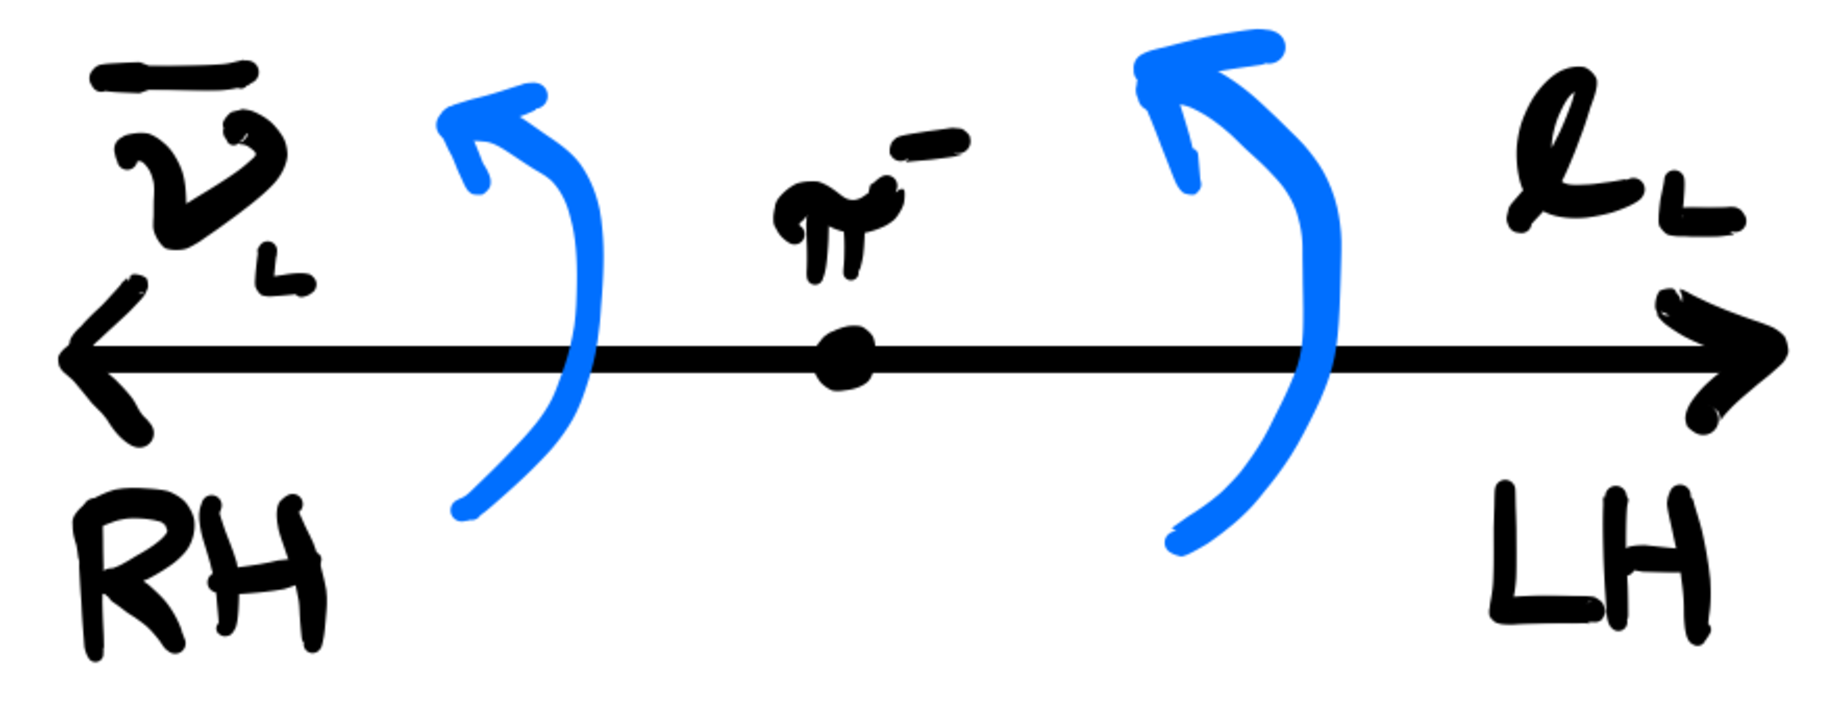
\includegraphics[width = .8\textwidth]{helicity_suppression}
		\caption{Helicities in $\pi^-\rightarrow\ell^-\overline\nu_\ell$ decay.}~
		\label{subfig:pi_helicity}
	\end{subfigure}
	~
	\begin{subfigure}[t]{.38\textwidth}
		\centering
		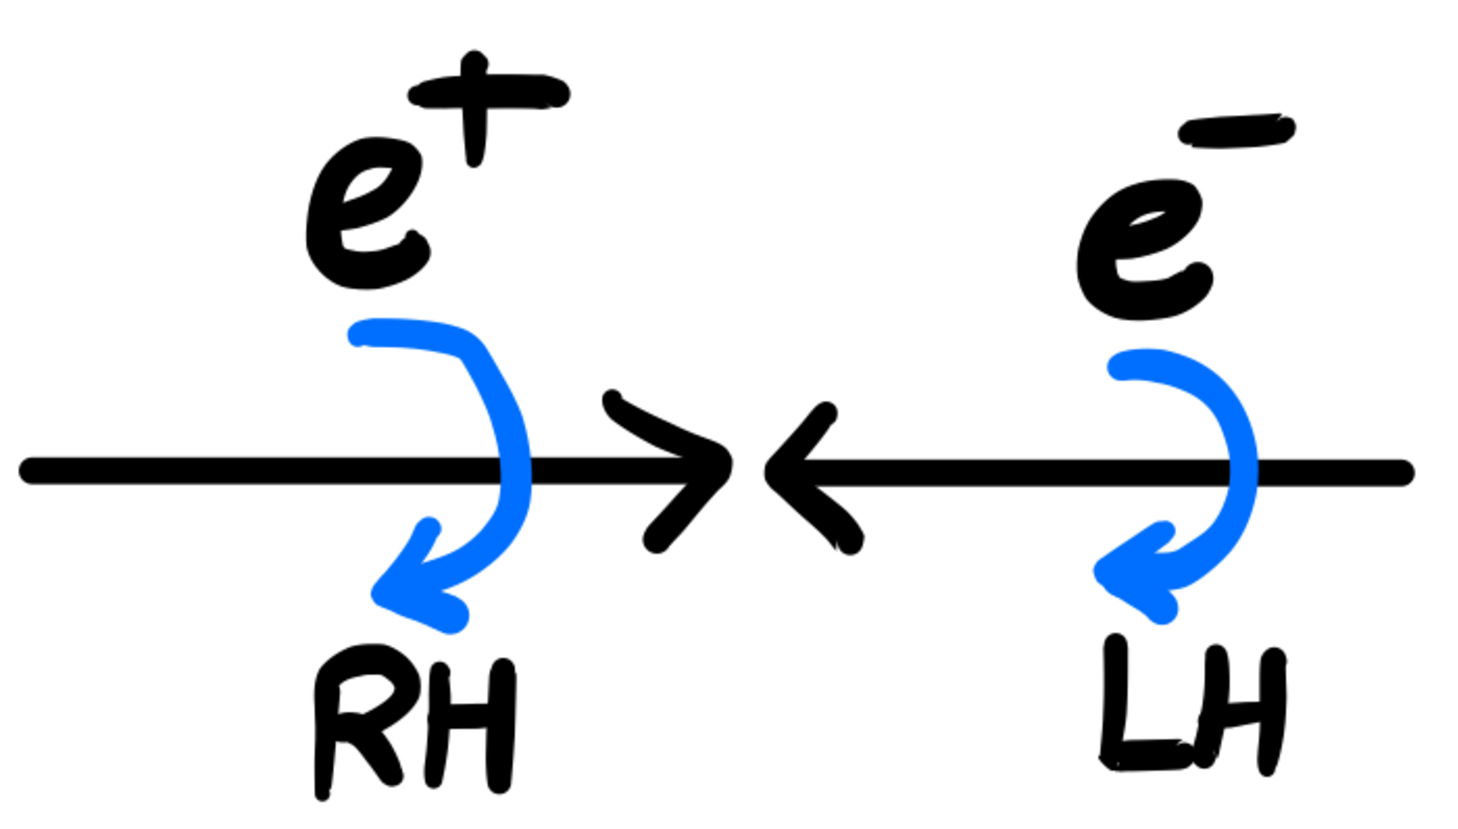
\includegraphics[width = .8\textwidth]{e+e-helicity}
		\caption{Helicities in $e^+ e^-$ annihilation.}~
		\label{subfig:e_helicity}
	\end{subfigure}
\end{figure}

There are a lot of tips and tricks associated with helicity arguments: we will study one in further detail in the next section when we study $e^+ e^-$ annihilation, but for now it suffices 
to note that the same mechanism implies that an $e^- e^+$ pair (or really, any pair of near massless Dirac particles / antiparticles) must carry some net angular momentum into 
the collision. Since the fields couple as $\overline e_R e_L$ and $\overline e_L e_R$, they have opposite chirality, hence opposite helicity, and this means that in their center of momentum 
frame their spins must be aligned, as in Figure~\ref{subfig:e_helicity}. Since they are oriented to have no net orbital angular momentum, the total angular momentum of the process is 
$J = 1$, which means that \textit{electron-positron annihilation can only create vector particles / resonances}. 

% TODO Yang's theorem and no spin 1 --> 2 spin 0 boson decays.

\subsection{Basics of colliders}

We begin by defining the parameters and observables that are necessary to describe the physics that occurs at colliders. 
Knowledge of the general parameters will allow us to make estimates of production rates at different colliders. The basic dimensional 
unit that is used at colliders is called the \textbf{barn}, which is defined as:
\begin{equation}
	1\;\mathrm{bn} = 10^{-28}\;\mathrm{m}^2.
\end{equation}
It is defined so that the nucleon-U$^{235}$ cross section is about equal to one barn: Fermi once said that having neutrons in a reactor hit 
a uranium-235 nucleus was as easy as hitting the side of a barn, which is where the name comes from. The other quantity we may need 
to keep in the back of our minds is the conversion factor from natural units to SI units: this conversion is done in terms of $\hbar c$. 
One can use that $(\hbar c)^2 = 3.894\times 10^{-32}\;\mathrm{m}^2\;\mathrm{GeV}^2$, but the easiest way to remember this conversion 
is that \textit{the radius of the proton is about a femtometer, and is about equal to $\Lambda_{\mathrm{QCD}}$, which is about 200 MeV}. This 
gives the conversion (and we record the factor for energy and time as well):
\begin{align}
	200\;\mathrm{MeV}\approx \frac{1}{\mathrm{fm}} && 1 \;\mathrm{GeV} \approx 1.52\times 10^{24}\;\frac{1}{\mathrm{sec}}
\end{align}

The setup that most colliders use is of colliding two beams $A$ and $B$, where each beam has $N_A$ and $N_B$ particles in it, respectively. 
The \textbf{center of mass energy} scale at a collider is just the typical $\sqrt s$ variable in the CoM frame
\begin{equation}
	\sqrt s = \sqrt{(p_A + p_B)^2}.
\end{equation}

When we look at collider processes, we will generally be looking to compute the scattering cross section $\sigma$, which gives us a 
probability. To relate this to experiment, we need an additional quantity called the \textbf{luminosity}. The luminosity comes in two 
forms: a \textit{differential} luminosity $L$, or an \textit{integrated} luminosity $L_\mathrm{int} = \int dt\; L$. The number of events that 
one sees at a collider is proportional to both the cross section of the process and the luminosity of the beam:
\begin{equation}
	N = \sigma L_\mathrm{int} = \sigma\int dt\; L
\end{equation}
Intuitively, the luminosity is a parameter that one can control by varying the shape, size, and density of the beam. A formula for the differential 
luminosity is:
\begin{equation}
	L = \frac{f N_A N_B}{\mathcal A}
\end{equation}
where $f$ is the frequency of revolution (for a circular collider), $N_A$ and $N_B$ are the numbers of particles in each beam, and 
$\mathcal A$ is the area of the beam. We see that one can increase the integrated luminosity in a few ways: adding more particles to the 
beam, increasing the frequency of revolution, decreasing the area, and also increasing the amount of time for a run. Changing any one of 
these parameters as specified makes the probability of a particle collision between the two beams more likely, hence why $L$ scales in this 
way. 

To put this jargon into play, here's a list of some common colliders to get a feel for what types of energies and processes 
we'll be looking into. Maxim Perelstein's TASI lectures~\cite{perelstein} have a good list; keep in mind these lectures were given in 2010, so 
some of the things here may be well out of date. We will mostly be considering the LHC for our examples as it is the most energetic 
particle collider in the world: however, there are other colliders of different types which also may reveal interesting physics.
\begin{table}[H]
	\centering
	\begin{tabular}{ | c | c | c | c | c | }
		\hline
		Collider & Type & Energy & $L_\mathrm{int}$ (pb$^{-1}$ / year) & Years \\
		\hline
		LHC & pp & 13 TeV & 10 K or 100 K & 2009 - present \\
		\hline
		Large Electron-Positron (LEP) & $e^+ e^-$ & $\approx 200$ GeV & 600 & 1989 - 2000 \\
		\hline
		HERA & $e^\pm p$ & 320 GeV & 500 & 1992-2007 \\
		\hline
		Tevatron & $p\overline p$ & 2 TeV & 6000 & 2000 - 2011 \\
		\hline
		Electron-Ion Collider (EIC) & $e$-ion & ? & ? & 2025? \\
		\hline
	\end{tabular}
	\caption{Table of some colliders in use around the world. Note that ``Energy" is the total energy involved in the collision in the 
	center of mass frame, $\sqrt s$. The energy per beam is $\sqrt s / 2$.}
	\label{table:colliders}
\end{table}
% LHC --> Higgs, Tevatron --> top, LEP --> precision measurements

The type of reaction the collider uses will determine the distribution of products formed in the collision. For example, the HERA collider 
measures the results of electron-proton collision, and its cross sections can therefore be computed using techniques from deep inelastic 
scattering. On the other hand, the LHC and tevatron use hadronic collisions to study new physics: instead of DIS, the process they 
use is Drell-Yan scattering. Some colliders also collide heavy ions together: the LHC occasionally does this, as well as the Relativistic Heavy 
Ion Collider (RHIC) and its soon-to-be successor, the EIC. Heavy ion collisions allow one to probe nuclear physics and to determine the 
ways that QCD influences the structure of the nucleon. 

A general rule of thumb is that \textit{hadronic colliders are used to discover new physics, while leptonic ones are used to refine other 
measurements}. This is because hadrons can be heuristically thought of as a ``bag of partons" where each parton has an energy that is not 
specified from the kinematics of the mother parton, so their interactions can encompass a wider range of parameter space than simply 
colliding together leptons. Once a discovery is made, typically at a hadronic collider, it is then refined at leptonic colliders. This paradigm 
can be seen in the colliders in the table: the Tevatron discovered the top quark and the LHC discovered the Higgs boson, but the LEP was 
primarily used for precision measurements of Standard Model parameters like $m_W$ and $m_Z$. 

This section is going to be a bit messy; there's a whole slew kinematical quantities used in collider physics, and I highly doubt we'll need to 
know more than transverse momentum / energy for the exam. When reading this, don't focus on the definitions themselves, instead try to 
get the broader picture of \textit{why} collider physicists care about these observables. 

Let's first briefly recall some formulas for the cross section and the decay rate in terms of the invariant matrix element $\mathcal M$ for the 
scattering process of interest. Since the collider's energy scale is typically $>>$ the other masses in the incoming / final states, it is 
often useful to take the massless limit for these particles. For \textit{two body decay in the CoM frame}:
\begin{align}
	d\Gamma = \frac{1}{32\pi^2} \frac{|\vec p_f|}{M^2}\,\overline{|\mathcal M|^2}\,d\Omega && 
	d\sigma = \frac{1}{64\pi^2 s}\frac{|\vec p_f|}{|\vec p_i|}\,\overline{|\mathcal M|^2}\,d\Omega  \nonumber
\end{align}
Furthermore, the energies of the colliders are so high that in these notes, we will \textbf{assume the incoming particles are massless, 
$m_A \approx m_B\approx 0$}. If we assume this and that the outgoing particles all have the same mass $m_1 = m_2 = m_f$, then 
the cross section formula is quite simple:
\begin{align}
	d\sigma = \frac{1}{64\pi^2 s}\sqrt{1 - \frac{4 m_f^2}{s}} \;\overline{|\mathcal M|^2} d\Omega && (\textnormal{Massless initial, equal mass 
	final}) 
\end{align}
Note that kinematically for this process to occur, we need to be \textbf{at the threshold}, $\sqrt s > m_1 + m_2$. Furthermore, when all the 
masses of the outgoing particles vanish, the square root factor vanishes and we have simply that:
\begin{align}
	d\sigma = \frac{1}{64\pi^2 s} \;\overline{|\mathcal M|^2} d\Omega && (\textnormal{All incoming/outgoing particles massless}) \nonumber
\end{align}

Collider data is often plotted against kinematical quantities which are invariant of a boost along the collider axis. 
Such variables have the same values in the lab frame and in the center of mass frame, and therefore there is no ambiguity when we work in 
either frame. The center of mass frame is shown in Figure~\ref{fig:kinematics}. A notable 
kinematical variable is the \textbf{transverse momentum} $\vec p_T$, which is simply the transverse portion of the three momentum of a 
particle:
\begin{equation}
	\vec p = (\vec p_T, p_z)
\end{equation}
where the $z$ axis is taken to be the direction of motion of the particles. The transverse momentum is a two vector $\vec p_T = (p_x, p_y)$ with norm $p_T := |\vec p_T|$. 

Another boost invariant is the \textbf{azimuthal angle}, which is simply the angle of the transverse momentum 
relative to the transverse plane, $\phi = \tan^{-1}\frac{p_x}{p_y}$. We can also study the \textbf{rapidity}:
\begin{equation}
	y = \frac{1}{2}\log\frac{E + p_z}{E - p_z}
\end{equation}
Under a boost, the rapidity transforms as $y\mapsto y + \log(\cos\beta + \sin\beta)$, where $\beta$ is the boost angle. The \textit{difference} 
in rapidities $y_1 - y_2$ thus clearly a boost invariant. 

\begin{figure}[H]
	\centering
	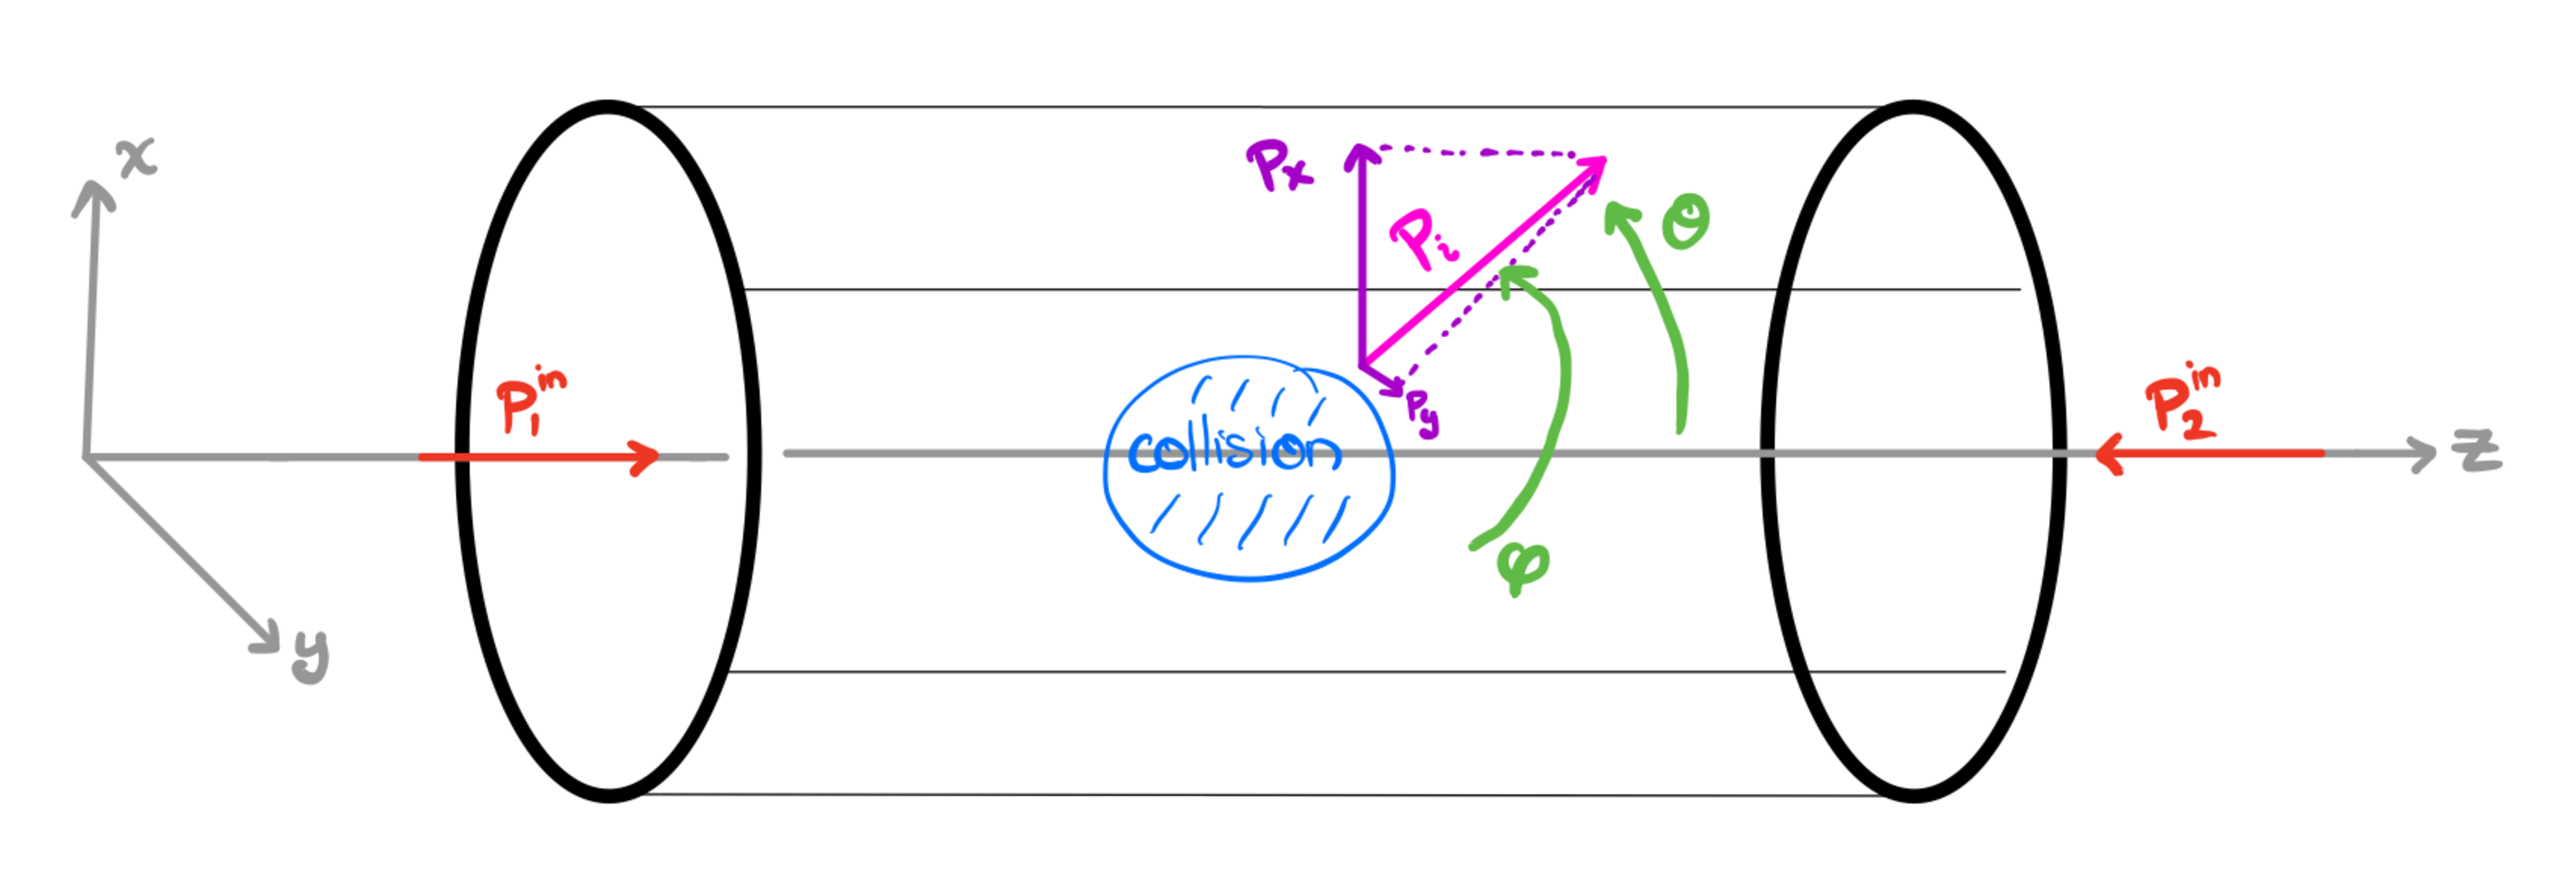
\includegraphics[width = 0.6\textwidth]{collider_kinematics}
	\caption{Kinematics of final-state momentum $\vec p$ in the center of mass frame. Note that $\phi$ is taken to be 0 on the $y$ axis instead of the $x$ axis as it's 
	technically defined, that's just an inconsistency in this drawing.}
	\label{fig:kinematics}
\end{figure}

The polar angle $\theta$ is often replaced with a coordinate $\eta$ called the \textbf{pseudorapidity}, which is defined as:
\begin{equation}
	\eta := \log\cot\frac{\theta}{2}\sim\frac{\pi}{2} - \theta + \mathcal O(\theta^2)
\end{equation}
where we have Taylor expanded $\eta$ for small values of $\theta$. This is a geometrical quantity which is typically used as a replacement for 
$\theta$ in collider data. If we consider the production of massless particles, $m_f = 0$, then the rapidity ends up precisely equalling the 
pseudorapidity. Nonetheless, the $\eta$ coordinate is used for all particles, despite the fact that it only has a clear kinematical interpretation 
for massless particles. $\eta$, as well as differences in $\eta$, is not a boost invariant when particles are not massless. 

We often abuse notation and define the \textbf{invariant mass} of a process:
\begin{equation}
	M^2 := \bigg|\sum_\textnormal{final states j} p_j^\mu\bigg|^2
\end{equation}
If the process features a parent decaying into daughters, this will give us the original mass of the parent particle, assuming all the daughters 
are measured. Furthermore, in a two particle collision this will equal the Mandelstam variable $s$. 
For a $1\rightarrow 2$ particle decay $A\rightarrow BC$ (this often happens in $W$ production and is how the mass of the W boson is 
measured) with final state transverse momenta $\vec p_T^{\;(1)}$ and $\vec p_T^{\;(2)}$, we define the \textbf{transverse energy} and 
\textbf{transverse mass} as:
\begin{align}
	E_T := \sqrt{M^2 + p_T^2} && m_T^2 := \left(E_T^{(1)} + E_T^{(2)}\right)^2 - \left(\vec p_T^{\;(1)} + \vec p_T^{\;(2)}\right)^2
\end{align}
where $M$ is the invariant mass of the process. If the final momenta are purely longitudinal ($\vec p_T^{\;(1)}$ and $\vec p_T^{\;(2)}$ are 0), 
then the transverse mass vanishes, and if the final momenta are purely transverse ($\vec p_T^{\;(1)} = \vec p^{\;(1)}$ and 
$\vec p^{\;(2)} = \vec p^{\;(2)}$) then the transverse mass equals the invariant mass. In any case, the transverse mass is always bounded by 
$0\leq m_T \leq m_A$, and when the bounds are saturated the daughters are either purely transverse or longitudinal. \textbf{The transverse 
mass is invariant upon boosting the parent particle $A$ along its collinear axis, and it is also not sensitive to transverse perturbations}: upon 
boosting $B$ or $C$ by a small parameter $\beta$ in the transverse plane, one can show that $m_T$ does not change at first order in 
$\beta$ and the first corrections are $m_T\mapsto m_T + \mathcal O(\beta^2)$. 

Let's turn our attention to what is actually measured at colliders. On paper, a collider event is completely defined by knowledge of the final 
state particles and their momenta; the final particle trajectories, once measured, can be extrapolated back to the collision point as long as 
their momenta are picked up in the detector. Since the detector is measuring final state particles at some length away from the collision point, 
it often happens that there are \textit{intermediate particles formed after the collision but before the final particles are picked up in the 
detector}. For example, in the Higgs discovery, the Higgs was created through gluon fusion and then decayed into two photons as 
$gg\rightarrow h\rightarrow\gamma\gamma$. When the LHC picked up this process, it did not measure the Higgs directly, but rather the two 
photons. Since they decayed from a real Higgs, their trajectories did not originate from the collision point, but rather from where the Higgs 
decayed. With complete knowledge of the final state momenta, we see that one can extrapolate what occurred to generate that final state, but 
it is by no means easy to establish this. 

Unfortunately, not all particles are picked up by detectors, and so complete knowledge of the final state is not always possible. Detectors are 
made to pick up energy deposits from a variety of particles, but the one type of particles that they will not pick up is \textbf{neutrinos}, since 
they are uncharged and don't interact with much. As such, we often measure the \textbf{missing transverse momentum / energy}
\begin{align}
	\slashed{\vec p_T} := - \sum_\textnormal{final states j} \vec p_T^{(j)} && \slashed{E_T} := |\slashed{\vec p_T}|
\end{align}
where the sum on $j$ picks up only the measured final states. Since $\sum \vec p_T = 0$ whens summing over all final states, $\slashed{\vec p_T}$ will give 
the sum of the transverse momenta of the final states which were not measured by the detector. For example in a $W^-\rightarrow e^-
\overline\nu_e$ decay, since there will be one missing particle (the neutrino), $\slashed{\vec p_T} = \vec p_T^{\;(\nu)}$ and we therefore know 
where the neutrino went after the collision. 

Detectors are typically made in layers, where each layer is able to track a particle with different hadronic or electronic 
properties~\cite{particle_detectors}. Once a detector triggers, as the particle passes through the different layers it deposits a different amount 
of energy in each layer it interacts with. There are three primary units which make up a detector; they are usually layered around the collision 
point in the following order, with the trackers being the innermost part and the muon detector being the outermost.
\begin{itemize}
	\item Trackers: Measures the momentum of charged particles.
	\item Calorimeters: Measures the energy of particles. Calorimeters can either be \textit{electric} or \textit{hadronic}: electric calorimeters 
	measure energies of photons and electrons, and hadronic calorimeters measure energies of hadrons. They are designed to stop any 
	particle other than a muon or a neutrino.
	\item Particle identifier: Identifies the type of particles which passes through based on determining what type of radiation the particle 
	emits.
	\item Muon detector: Muons don't interact very much with matter. They are very fast and require a lot of material to stop them, and 
	chambers to identify muons and track them usually make up the outer layer of most detectors. 
\end{itemize}

Particle detectors also have finite resolution: in general, particles need to travel far enough in the detector to be identified. The 
\textbf{spatial resolution} of a detector is how far apart two particles need to be for the detector to resolve them as distinct: typically this 
is on the order of 10 to 100 $\mu$m. Likewise, the \textbf{time resolution} of a detector is the amount of time required to resolve two 
distinct events, and is also the smallest amount of time a particle's lifetime (in the \textit{lab frame}; since particles are moving so fast there 
is usually significant time dilation between the rest frame lifetime $\tau$ and the lab frame lifetime $\gamma\tau$) must be to be picked up by 
the detector. In modern detectors, the time resolution is typically on the order of nanoseconds to microseconds.


\subsection{Electron-positron annihilation}

%\newpage
%\section{Yang-Mills theory and differential forms}~
%\label{sec:topology}

%Yang-Mills action:
%\begin{equation}
%	S = \frac{1}{4\pi} \int F\wedge *F
%\end{equation}
%since the Hodge star moves the pieces around appropriately. Note that the $\epsilon^{\mu\nu\alpha\beta} F_{\mu\nu} F_{\alpha\beta}$ is 
%just $F\wedge F$, which makes sense because characteristic classes must be defined as a wedge product of the curvature. 

\newpage
\section{Appendix: Formulas and quantities to memorize}

\subsection{Masses and charges of SM and common hadrons}

\begin{itemize}
	
	\item Mass and the mass hierarchy of Standard Model particles. 
	\begin{table}[H]
	\centering
	\begin{tabular}{ | c | c | c | c | c | c | c | c | }
		\hline
		$\nu$ & e & u & d & s & $\mu$ & $\pi^0$ & $\pi^\pm$ \\
		\hline
		$\approx 0$ & 0.511 MeV & 2.2 MeV & 4.7 MeV & 93 MeV & 110 MeV & 134 MeV & 139 MeV \\
		\hline
		\end{tabular}
		\begin{tabular}{ | c | c | c | c | c | c | c | c | c | }
		\hline
		$p^+$ & $n^0$ & c & $\tau$ & b & W & Z & H & t \\
		\hline
		938 MeV & 939 MeV & 1.3 GeV & 1.8 GeV & 4.2 GeV & 80 GeV & 91 GeV & 125 GeV & 173 GeV \\
		\hline
	\end{tabular}
	\end{table}
	
	\item Approximate meson masses:
	\begin{table}[H]
	\centering
	\begin{tabular}{ | c | c | c | c | c | }
		\hline
		Meson & $\pi$ & $K$ & $D$ & $B$ \\
		\hline
		Quark content & $u\overline d$ & $s\overline q$ & $c\overline q$ & $b\overline q$ \\
		\hline
		Approximate mass & 140 MeV & 500 MeV & 1.8 GeV & 5.2 GeV \\
		\hline
		\end{tabular}
	\end{table}
	
	\item Charges of Standard Model particles:
	\begin{table}[H]
	\centering
	\begin{tabular}{ | c | c | c | c | c | }
		\hline
		Particle & SU(3) & SU(2) & U(1) & Lorentz \\
		\hline
		$Q_L = \begin{pmatrix} u_L \\ d_L \end{pmatrix}$ & \textbf{3} & \textbf{2} & $1/6$ & $(1/2, 0)$ \\
		\hline
		$u_R$ & \textbf{3} & 1 & $2/3$ & $(0, 1/2)$ \\
		\hline
		$d_R$ & \textbf{3} & 1 & $-1/3$ & $(0, 1/2)$ \\
		\hline
		$\ell_L = \begin{pmatrix} \nu_L \\ e_L \end{pmatrix}$ & 1 & \textbf{2} & $-\frac{1}{2}$ & $(1/2, 0)$ \\
		\hline
		$e_R$ & 1 & 1 & -1 &  $(0, 1/2)$ \\
		\hline
		$\nu_R$ & 1 & 1 & 0 & $(0, 1/2)$ \\
		\hline
		H & 1 & \textbf{2} & $1/2$ & $(0, 0)$ \\ 
		\hline
	\end{tabular}
	\end{table}
	
	\item Masses and quantum numbers of light hadrons:
	\begin{table}[H]
	\centering
	\begin{tabular}{ | c | c | c | c | c | c | }
		\hline
		Meson & $\pi^0, \pi^\pm$ & $K^+$, $K^0$, & $K^-$, $\overline K^0$ & $\eta$ & $\eta'$ \\
		\hline
		Mass (MeV) & 140 & 500 & 500 & 550 & 950 \\
		\hline
		Quark content & $u\overline d$, $d\overline u$, $u\overline u - d\overline d$ & $u\overline s$, $d\overline s$ & $s\overline u$, $s\overline d$ & $u\overline u + d\overline d - 
		2 s\overline s$ & $u\overline u + d\overline d + s\overline s$ \\
		\hline
	\end{tabular}
	\caption{Pseudoscalar nonet, spin 0, $P = -$, grouped into isospin multiplets.}
	\label{table:pseudoscalar_nonet}
	\end{table}
	
	\begin{table}[H]
	\centering
	\begin{tabular}{ | c | c | c | c | c | c | }
		\hline
		Baryon & $n^0$ & $p^+$ & $\Sigma$ & $\Xi$ & $\Lambda^0$ \\
		\hline
		Mass (MeV) & 939 & 938 & 1190 & 1315 & 1116  \\
		\hline
		Strangeness & 0 & 0 & -1 & -2 & -1 \\
		\hline
		Charge & 0 & 1 & $\pm 1, 0$ & $-1, 0$ & 0 \\
		\hline
		Quark content & udd & uud & uus, uds, dds & dss, uss & uds \\
		\hline
	\end{tabular}
	\caption{Baryon octet, spin $\frac{1}{2}$, $P = +$. Isospin multiplets are $(p, n)$, $(\Sigma^\pm, \Sigma^0)$, and $(\Xi^0, \Xi^-)$. Note the 
	mass splittings are about 150 to 200 MeV.}
	\label{table:baryon_octet}
	\end{table}
	
	% Baryon decuplet
	
	% vector mesons
	
	%\item Approximate values of couplings and their units:
	% G_F, \alpha_s, g_2, \alpha_EM, \theta_W (or sin^2\theta_W), \Lambda_{QCD}
	
	
	\newpage
	\subsection{Units, conversions, decays, and cross sections}
	\item Units:
	\begin{align}
		\hbar c = 197.326 \;\mathrm{MeV} \cdot \mathrm{fm} && c = 3\times 10^8 \frac{m}{s}
	\end{align}
	Ex: to get energy from a mass $M$ with $[M] = 1$, multiply by $c^2$. To get an energy from a length, divide by $\hbar c$. 
	\item $\Lambda_\mathrm{QCD}$ is the location of the Landau pole in the QCD $\beta$ function and arises from dimensional 
	transmutation:
	\begin{equation}
		\Lambda_\mathrm{QCD}\approx 200\;\mathrm{MeV}
	\end{equation}
	\item \textbf{Conversion factors} ($\Lambda_\mathrm{QCD}\approx r_p^{-1}\approx 1 \;\mathrm{fm}^{-1}$):
	\begin{align}
		\hbar &= 6.58\times 10^{-16} \;\mathrm{eV}\cdot\mathrm{sec} \approx 5\times 10^{-16} \;\mathrm{eV}\cdot\mathrm{sec} \\
		\hbar c &= 197.326 \;\mathrm{MeV} \cdot \mathrm{fm}\approx \Lambda_\mathrm{QCD}\cdot\mathrm{fm} \\
		1 \;\mathrm{GeV}^{-1} &\approx 6.58\times 10^{-25}\;\mathrm{sec}\approx 0.2 \;\mathrm{fm}
	\end{align}
	
	\item Dimensions of fields:
	\begin{align}
		[\phi] = [A_\mu] = \frac{d - 2}{2}\xrightarrow{d = 4} = 1 && [\psi] = \frac{d - 1}{2} \xrightarrow{d = 4} \frac{3}{2}
	\end{align}
	
	\item Dimensions of $\delta$ function: Always inverse of its 
	argument\footnote{https://physics.stackexchange.com/questions/33760/what-are-the-units-or-dimensions-of-the-dirac-delta-function}.
	\begin{equation}
		[\delta(x)] = -[x] = \left[\frac{1}{x}\right]
	\end{equation}
	
	\item Lorentz invariant phase space:
	\begin{equation}
		d\Pi_\mathrm{LIPS} = (2\pi)^4 \delta^{(4)}\left(\sum p\right) \prod_{\textnormal{final states } j} \frac{d^3\vec k_j}{(2\pi)^3} \frac{1}{2 E_j}
	\end{equation}
	Decay rate and cross section formulas:
	\begin{align}
		d\Gamma = \frac{1}{2 M} \overline{|\mathcal M|^2} d\Pi_\mathrm{LIPS} && \tau = \frac{1}{\Gamma} && d\sigma = \frac{1}{4 E_1 E_2 |\vec v_1 - \vec v_2|}\,
		\overline{|\mathcal M|^2}\,d\Pi_\mathrm{LIPS}
	\end{align}
	where $E_1$ and $E_2$ ($v_1$ and $v_2$) are the energies (velocities) of the incoming particles in the frame you are working in. For $d\Gamma$, in the rest frame $E_1$ is simply 
	the mass $M$ of the decaying particle. Note the velocity is $\vec v = \frac{\vec p}{p^0}$. These equations simplify in certain cases:
	\begin{align}
		d\Gamma = \frac{1}{32\pi^2} \frac{|\vec p_f|}{M^2}\,\overline{|\mathcal M|^2}\,d\Omega && (1\rightarrow \textnormal{2 body decay}) \\
		d\sigma = \frac{1}{64\pi^2 E_\mathrm{CM}^2}\frac{|\vec p_f|}{|\vec p_i|}\,\overline{|\mathcal M|^2}\,d\Omega && (2\rightarrow \textnormal{2 body decay, CoM frame})
	\end{align}
	\begin{align}
	d\sigma = \frac{1}{64\pi^2 s}\sqrt{1 - \frac{4 m_f^2}{s}} \;\overline{|\mathcal M|^2} d\Omega && (2\rightarrow 2 \textnormal{ CoM, initial mass zero, final mass equal}) 
	\end{align}
	
	\item Dimensions of kinematical variables: Note that \textit{the invariant matrix element is only dimensionless for four particle scattering}
	\footnote{https://physics.stackexchange.com/questions/452119/mass-dimension-of-an-n-particle-scattering-amplitude-in-4d?fbclid=IwAR0Vw2Ibf6dly8H4137qdwmU-XGzhXbkeF9MVcmNLVTbHNGm4PJiXkGwdjs}:
	\begin{equation}
		[\mathcal M] = 4 - (\textnormal{number of total particles})
	\end{equation}
	Cross section and decay rate:
	\begin{align}
		[\sigma] = [\mathrm{Area}] = -2 && [\Gamma] = 1
	\end{align}
	One-particle states $|\vec p\rangle$ have dimension $-1$ because of the normalization $\langle p | p'\rangle = 2 m \delta^{(3)}(p - p')$. 
	
	\item Units and the definition of luminosity:
	\begin{align}
		1\;\mathrm{bn} = 10^{-28} \;\mathrm{m}^2 && N = \sigma L_\mathrm{int} && \sigma(pp; \;\mathrm{inclusive})\sim 30 mbn
	\end{align}
	The LHC has a luminosity of $10K$ (low) or $100K$ (high) $pb^{-1} / \mathrm{year}$ and a collision energy of $\sqrt S = 13$ TeV.
	
	\item \textbf{Approximating the phase space integral}: $f =$ number of final state particles:
	\begin{equation}
		\Gamma\sim \frac{1}{2}(2\pi)^4 \left(\frac{1}{2 (2\pi)^3}\right)^{f} (2\pi)^{f - 1} |\mathcal M|^2 \Lambda
	\end{equation}
	
	\item Loop factors: Loops are typically suppressed by an order of about:
	\begin{equation}
		\frac{1}{16\pi^2} = 0.006\approx \frac{1}{100}
	\end{equation}
	times the coupling squared. This comes from doing the integral out after Wick rotation.
	
	\item Bohr radius and energy levels of Hydrogen (useful for quarkonia):
	\begin{align}
		r_B = \frac{1}{\alpha \mu} && E_0 = \frac{\alpha}{r_B} = \alpha^2\mu
	\end{align}
	where $\mu$ is the reduced mass of the system. 
	
	\item Breit-Wigner distribution: Near a resonance of particle $X$, the cross section goes as:
	\begin{equation}
		\sigma \propto \frac{1}{(s - m_X^2)^2 + m_X^2 \Gamma_X^2}\approx \frac{\pi}{m_X\Gamma_X}\delta(s - m_X^2)
	\end{equation}
	where $\Gamma_X$ is the total decay width of species $X$, and the last $\approx$ is the \textbf{narrow width 
	approximation} which is valid for $\Gamma_X << m_X$. 
	
	\item Helicity suppression: Primarily occurs in decays of pseudoscalars to fermions, for example $\pi^-\rightarrow\ell^-
	\overline\nu_\ell$. In the massless limit the helicities of $\ell$ and $\overline\nu_\ell$ are LH and RH, respectively, and 
	in the CoM frame for $\pi^-$ this implies the final state has total angular momentum of $J = 1$; this violates conservation of 
	angular momentum since $\pi^-$ has no spin. Therefore $\Gamma(\pi\rightarrow\ell\nu_\ell)\propto m_\ell^a$ for some nonzero 
	$a$, since the decay has to turn off as $m_\ell\rightarrow 0$. 
	
	\item OZI rule: Diagrams which can be separated into initial / final states by cutting only gluon lines are suppressed. 
	
	\item Statistics: A state with identical particles of total angular momentum $J$ has $(-)^J$ under interchange of the particles. This implies that 
	a spin 1 particle cannot decay into two spin 0 bosons, as they would be required to be symmetric under interchange but $(-)^{J = 1} = -$ 
	(forbids the $Z\rightarrow hh$ and $\rho^0\rightarrow\pi^0\pi^0$ decays).
	
	\newpage
	\subsection{Spinors}
	
	\item Dirac matrices (Weyl basis):
	\begin{align}
		\gamma^0 = \begin{pmatrix} 0 & 1 \\ 1 & 0 \end{pmatrix} && \gamma^i = \begin{pmatrix} 0 & i\sigma^i \\ i\sigma^i & 0 \end{pmatrix} && \gamma_5 = \begin{pmatrix} -1 & 0 \\ 
		0 & 1 \end{pmatrix}
	\end{align}
	
	\item Spinor sums and technology: note that $[u] = [v] = \frac{1}{2}$ by the normalization.
	\begin{align}
		\overline u_{ps} u_{ps'} = 2m\delta_{ss'} && \overline v_{kr} v_{kr'} = -2m\delta_{rr'} \\
		\sum_s u_{ps}\overline u_{ps} = \slashed p + m && \sum_s v_{ps}\overline v_{ps} = \slashed p - m \\
		\gamma_5 = i\gamma^0 \gamma^1 \gamma^2\gamma^3 && \sigma^{\mu\nu} = \frac{i}{2}[\gamma^\mu, \gamma^\nu] \\
		\{\gamma^\mu, \gamma^\nu\} = 2 g^{\mu\nu} && \{\gamma^\mu, \gamma_5\} = 0 \\
		\gamma^\mu \gamma_\mu = 4 && \gamma^\mu\gamma^\nu\gamma_\mu = -2\gamma^\nu  \\
		tr\{\gamma^\mu\gamma^\nu\} = 4 g^{\mu\nu} && tr\{\textnormal{odd \# of }\gamma s\} = 0
	\end{align}
	\begin{align}
		tr\{\gamma^\mu\gamma^\nu\gamma^\rho\gamma^\sigma\} &= 4(g^{\mu\nu} g^{\rho\sigma} - g^{\mu\rho} g^{\nu\sigma} + g^{\mu\sigma} g^{\nu\rho}) \\
		tr\{\gamma^\mu\gamma^\nu\gamma^\rho\gamma^\sigma\gamma_5\} &= -4i\epsilon^{\mu\nu\rho\sigma}
	\end{align}
	
	\item On-shell spinor identities and the magnetic moment:
	\begin{align}
		\slashed{p} u(p) = m u(p) && (\textnormal{Dirac eqn}) \\
		\overline u(q) \gamma^\mu u(p) = \overline u(q)\left[ \frac{q^\mu + p^\mu}{2m} + i\sigma^{\mu\nu} \frac{(q^\nu - p^\nu)}{2m} \right] u(p) && 
		(\textnormal{Gordon identity})
	\end{align}
	The magnetic moment measures the operator $F_{\mu\nu} \sigma^{\mu\nu}$. 
	
	\item Discrete symmetries of the SM: Matrices used in $C$ symmetry:
	\begin{align}
		\mathcal C = \begin{pmatrix} \epsilon_{ab} & 0 \\ 0 & \epsilon^{ab} \end{pmatrix} && \epsilon_{ab} = \begin{pmatrix} 0 & 1 \\ -1 & 0 \end{pmatrix} && \epsilon^{ab} = \begin{pmatrix} 0 & -1 \\ 1 & 0 \end{pmatrix}
	\end{align}
	$C$ and $P$ transformation laws ($x_P := P_\mu^\nu x_\nu = (x^0, -\vec x)$):
	\begin{align}
		P \phi(x) P^* = \phi(x_P) && C \phi(x) C^* = \phi^*(x) && (\textnormal{Scalar field}) \\
		P \psi(x) P^* = \gamma^0 \psi(x_P) && C \psi(x) C^* = \mathcal C\overline{\psi}^T(x) = -i\gamma^2\psi^*(x) && (\textnormal{Spin-1/2 field}) \\
		P A_\mu^a(x) t^a P^* = P^\mu_\nu A_\nu^a(x_P) t^a && C A_\mu^a(x) t^a C^* = - \left[A_\mu^a(x) t^a\right]^* && (\textnormal{Spin-1 field})
	\end{align}
	The $-$ on the gauge field $C$ transformation comes from desiring $-i A_\mu$ to transform the same as $\partial_\mu$ in $D_\mu$. There are a few 
	ways to remember the action of $C$ on Dirac spinors, but the easiest is to remember that it interchanges the two particles and adjusts the 
	indices appropriately:
	\begin{equation}
		\psi(x) = \begin{pmatrix} \chi_a \\ \xi^{\dagger\dot a} \end{pmatrix}\xrightarrow{C} \begin{pmatrix} \xi_a \\ \chi^{\dagger\dot a}\end{pmatrix}
	\end{equation}
	
	\item \textbf{Action of C and P on Dirac bilinears}: We are working here with the bilinears $S = \overline\psi\psi$, $P = \overline\psi\gamma_5\psi$, 
	$V = \overline\psi\gamma^\mu\psi$, $A = \overline\psi\gamma^\mu\gamma_5\psi$, and $T = \overline\psi\sigma^{\mu\nu}\psi$. $P$ acts on them as it 
	would on a normal vector:
	\begin{align}
		S\mapsto S && P\mapsto -P && V_0\mapsto V_0, V_i\mapsto -V_i && A_0\mapsto -A_0, A_i\mapsto A_i
	\end{align}
	$C$ is a bit more complicated. The pseudoscalar and axial vectors transform nicely under $C$ when multiplied by $i$, and the only other thing to remember 
	is that $C$ inverts the vector (so $A_\mu \overline\psi\gamma^\mu\psi$ is invariant, as $A$ is negative under $C$):
	\begin{align}
		S\mapsto S && iP\mapsto iP && V\mapsto -V && iA\mapsto iA
	\end{align}
	
	\item \textbf{Dirac conjugation}: For Dirac spinors, note the conjugate has opposite indices as $\Psi$ so we can contract them together:
	\begin{align}
		\Psi = \begin{pmatrix} \chi_a \\ \xi^{\dagger\dot a}\end{pmatrix} && \overline\Psi = \Psi^\dagger\gamma^0 = \begin{pmatrix} \xi^a && \chi^\dagger_{\dot a} \end{pmatrix}
	\end{align}
	
	% photon spin angular momentum: https://physics.stackexchange.com/questions/105121/addition-of-spin-angular-momentum-for-massless-particles
	
	\item Continuous symmetries of the SM: Baryon and lepton number. $U(1)_B$ rotates each quark field via $q\mapsto e^{i\theta B} q$ and 
	leaves everything else untouched ($B q = \frac{1}{3} q$ and $B \overline q = -\frac{1}{3} \overline q$). $U(1)_e$, $U(1)_\mu$, and 
	$U(1)_\tau$ rotate their appropriate lepton field $\ell_i$ in the same way; there are three of them in the SM because neutrinos don't have 
	mass, but with the PMNS matrix included them only total lepton number $U(1)_L$ is conserved. Both baryon and lepton number are anomalous, 
	but $B - L$ is not anomalous (if right-handed neutrinos are introduced to the SM). 
	% baryon number, lepton number, etc. (include U(1)_B-L anomaly)
	
	\item \textbf{Spin $\frac{1}{2}$ mass terms}: 
	\begin{itemize}
		\item Weyl spinors $\psi_L$ and $\psi_R$:
		\begin{equation}
			m_L \epsilon^{ab}\psi_{L, a}\psi_{L, b} + m_R \epsilon_{\dot a\dot b} \psi_R^{\dot a} \psi_R^{\dot b}
		\end{equation}
		\item Dirac spinors $\Psi_D = \begin{pmatrix} \psi_L \\ \psi_R \end{pmatrix}$:
		\begin{equation}
			m_D\overline\Psi_D\Psi_D = m_D(\overline\psi_R \psi_L + \overline \psi_L \psi_R) = m_D(\psi_R^{\dagger a} \psi_{L, a} + \psi_{L, \dot a}^\dagger \psi_R^{\dot a})
		\end{equation}
		where $\overline\psi_L$, $\overline\psi_R$ are taken when these Weyl spinors are embedded in Dirac spinors with definite chirality (\textit{not Majorana spinors}). 
		\item Majorana spinors: $\Psi_M = \begin{pmatrix} \psi_{a} \\ \psi^{\dagger, \dot a} \end{pmatrix}$, where $\psi$ is a LH Weyl spinor in $(\frac{1}{2}, 0)$:
		\begin{equation}
			m_M \overline\Psi_M \Psi_M = m_M (\psi^a \psi_a + \psi^\dagger_{\dot a} \psi^{\dagger\dot a})
		\end{equation}
	\end{itemize}
	
	\newpage
	\subsection{The Standard Model}
	
	\item Basic representation theory for $SU(N)$ and Yangs-Mill identities:
	\begin{align}
		[t^a, t^b] = i f^{abc} t^c && \left(T_\mathrm{ad}^a\right)^{bc} = -i f^{abc} && \mathrm{tr}[t^a t^b] = T(R) \delta_{ab}, \;T(\mathrm{fund}) = \frac{1}{2} \nonumber \\
		D_\mu = \partial_\mu - i g A_\mu && F_{\mu\nu} = \partial_\mu A_\nu - \partial_\nu A_\mu - ig [A_\mu, A_\nu] && F_{\mu\nu}^a = 2\mathrm{tr}[t^a F_{\mu\nu}] \nonumber \\
		A_\mu\mapsto U^\dagger A_\mu U + \frac{i}{g} U^\dagger \partial_\mu U && F_{\mu\nu}\mapsto U F_{\mu\nu} U^\dagger
	\end{align}
	
	\item Form of the $SU(N_c)$ Yang-Mills $\beta$ function with $n_f$ fermions:
	% Include relations between \beta_n and \alpha_s, and how \alpha_s relates to the coupling
	\begin{align}
		\beta = -2\alpha \sum_{n = 0}^\infty \beta_n \left(\frac{\alpha}{4\pi}\right)^{n + 1} && \alpha = \frac{g^2}{4\pi} &&
		\beta_0 = \frac{11}{3} N_c - \frac{2}{3} n_f 
	\end{align}
	For QCD, $N_c = 3$ and $C_A = 3$, $C_F = \frac{4}{3}$, and $T_F = \frac{1}{2}$.
	
	\item Standard Model Lagrangian: 
	\begin{align}
	\mathcal{L}_\mathrm{Gauge} &= -\frac{1}{4} B_{\mu\nu} B^{\mu\nu} - \frac{1}{4} W_{\mu\nu}^a W^{\mu\nu a} - \frac{1}{4} 
	G_{\mu\nu}^A G^{\mu\nu A} + \theta_\mathrm{QCD} \epsilon^{\mu\nu\alpha\beta} G_{\mu\nu} G_{\alpha\beta} \\
	\mathcal{L}_\mathrm{Fermi} &= i\sum_\psi\overline\psi \slashed D \psi = i\sum_{\psi_L} \overline\psi_L 
	\overline\sigma^\mu D_\mu\psi_L + i\sum_{\psi_R} \sigma^\mu D_\mu \psi_R \\
	\mathcal{L}_\mathrm{Higgs} &= D_\mu H D^\mu H^\dagger + \mu^2 H^\dagger H - \lambda (H^\dagger H)^2 \\
	\mathcal{L}_\mathrm{Yukawa} &= - Y_{ij}^d \overline Q_L^i H d_R^j - Y_{ij}^u \overline Q_L^i\epsilon H^* u_R^j - 
	Y_{ij}^e \overline\ell_L^i H e_R^j \\
	D_\mu &= \partial_\mu - i g' B_\mu - ig W_\mu^a t^a - ig_3 G_\mu^A T^A
	\end{align}
	% Mostly just want form of Yukawa couplings
	
	\item Value of SM couplings (all couplings are measured at scale $\mu_{\overline{MS}} = m_Z$):
	\begin{align}
		\sin^2\theta_w \sim .2229 && v = 247\;\mathrm{GeV} && \Theta_\mathrm{QCD}\approx 0 \\
		g' = 0.357 && g = 0.652 && g_3 = 1.221 \\
		\alpha_\mathrm{EM}\approx\frac{1}{129} &&  && \alpha_\mathrm{s} \approx 0.12
	\end{align}
	The Higgs vev $v$ can be measured through computing $G_F$ through muon decay in the 4-Fermi theory. Note it is easier to remember 
	$G_F\approx 10^{-5}\;\mathrm{GeV}^{-2}$ and solve for $g\approx 0.6$, and for $\alpha_s$ you can remember from lattice computations 
	it runs from about $0.1$ at $m_Z$ to about $0.3$ at $\mu = 2\;\mathrm{GeV}$. 
	
	\item Angles and CP violating phase in the CKM matrix:
	\begin{align}
		\theta_{12} = 13.1^\circ && \theta_{13} = 0.2^\circ \\
		\theta_{23} = 2.4^\circ && \delta = 0.995 \;\mathrm{rad}
	\end{align}
	
	\item \textbf{SSB and Goldstone's theorem}: Lagrangian invariant under $G$, condensate invariant under $H\subset G$, we say 
	\textbf{the symmetry spontaneously breaks $G\rightarrow H$}. Creates $|G| - |H|$ massless Goldstone bosons $\{\pi^a(x)\}_{a = 1}^{|G / H|}$ 
	which parameterize the quotient space $G / H$. These Goldstone modes couple to the broken currents $\{J^{\mu a}\}$ as:
	\begin{equation}
		\langle 0 | J^{\mu a}(x) | \pi^b(p)\rangle = i f_\pi p^\mu \delta^{ab} e^{-ipx}
	\end{equation}
	$J^{\mu a}$ is generated by the broken symmetry $\phi\mapsto U(\theta^a)\phi$, under which the Goldstone modes transform 
	via a shift, $\pi^a\mapsto \pi^a + f_\pi\theta^a$ (use the exponential rep). This implies \textit{the Goldstone bosons can only be 
	derivatively coupled}, since $\mathcal L$ must be invariant under this transformation but $\pi^a$ transforms as a translation.
	
	\item Relation between electroweak parameters / masses:
	\begin{align}
		m_W = \frac{gv}{2} && m_Z = \frac{v}{2}\sqrt{g^2 + (g')^2} && m_W = m_Z\cos\theta_w \\
		e = g\sin\theta_w && \tan\theta_w = \frac{g'}{g} && \cos\theta_w = \frac{g}{\sqrt{g^2 + (g')^2}}
	\end{align}
	% including custodial SU(2)
	
	\item \textbf{Electroweak covariant derivative after symmetry breaking}:
	\begin{equation}
		D_\mu = \partial_\mu -i \frac{g}{\sqrt 2} (W_\mu^+ t^+ + W_\mu^- t^-) + \left(\frac{g}{\cos\theta_w}\right) (t^3 - 
		Q\sin^2\theta_w) Z_\mu + e A_\mu Q
	\end{equation}
	
	\item \textbf{Electroweak charged and neutral currents}:
	\begin{align}
		\mathcal L_\mathrm{EW, int} &= \sum_f \overline\psi_f i\slashed\partial\psi_f + \frac{g}{\sqrt 2} \left( W_\mu^+ j_\mathrm{CC}^{\mu 
		+} + W_\mu^- j_\mathrm{CC}^{\mu -} \right) + \frac{g}{\cos\theta_w} Z_\mu j_\mathrm{NC}^\mu + e A_\mu j_\mathrm{EM}^\mu \\
		&= \sum_f \overline\psi_f i\slashed\partial\psi_f + \frac{e}{\sqrt 2\sin\theta_w} \left( W_\mu^+ j_\mathrm{CC}^{\mu 
		+} + W_\mu^- j_\mathrm{CC}^{\mu -} \right) + \frac{e}{\cos\theta_w\sin\theta_w} Z_\mu j_\mathrm{NC}^\mu + e A_\mu 
		j_\mathrm{EM}^\mu
	\end{align}
	The currents are:
	\begin{align}
	j_{\textnormal{CC}}^{\mu +} &= \overline u^i \gamma^\mu V^{ij}_\mathrm{CKM} P_L d^j +  \overline\nu_e \gamma^\mu P_L e + \overline\nu_\mu \gamma^\mu P_L \mu + \overline\nu_\tau \gamma^\mu P_L \tau \\
	j_{\textnormal{CC}}^{\mu -} &= \overline d^i \gamma^\mu (V_\mathrm{CKM}^\dagger)^{ij} P_L u^j + \overline e \gamma^\mu 
	P_L\nu_e + \overline \mu \gamma^\mu P_L \nu_\mu + \overline\tau \gamma^\mu P_L\nu_\tau = (j_\mathrm{CC}^{\mu +})^\dagger  
	\\
		j_\mathrm{NC}^\mu &= \sum_f \overline\psi_f \gamma^\mu \left(t^3 P_L - Q_f\sin^2\theta_w \right) \psi_f \\
		j_\mathrm{EM}^\mu &= \sum_f Q_f \overline \psi_f \gamma^\mu\psi_f
	\end{align}
	The neutral current is often written in terms of an axial and vector coupling as:
	\begin{equation}
		\mathcal L_\mathrm{NC} = \frac{e}{\sin\theta_w \cos\theta_w} Z_\mu \sum_f \overline\psi_f \left(g_V^{(f)}\gamma^\mu - 
		g_A^{(f)}\gamma^\mu\gamma_5\right) \psi_f
	\end{equation}
	where the couplings are specific to each fermion type and equal:
	\begin{align}
		g_V^{(f)} = \frac{1}{2} t^3_f - Q_f\sin^2\theta_w && g_A^{(f)} = \frac{1}{2} t^3_f
	\end{align}
	
	\item \textbf{CKM Matrix}: Wolfenstein parameterization ($\lambda = \sin\theta_w\approx 0.22$). Remember that decays which 
	change the generation by 2 are the most suppressed, so $\lambda^3$ is in the top and bottom corners; similarly, the smallest 
	suppression of the suppressed decays are within the first two generations. 
	\begin{equation}
	V_\mathrm{CKM} = \begin{pmatrix} 1 - \frac{\lambda^2}{2} & \lambda & \lambda^3 \\
	-\lambda & 1 - \frac{\lambda^2}{2} & \lambda^2 \\
	\lambda^3 & \lambda^2 & 1
	\end{pmatrix}
	\end{equation}
	Jarlskog invariant and unitary triangle:
	
	\item \textbf{PMNS matrix}: Approximate sizes of entries and angles:
	\begin{align}
		|\nu_a\rangle = U_{ai} |\nu_i\rangle
	\end{align}
	TODO approx neutrino masses ($m_{\nu_i} < 1\;\mathrm{eV}$). 
	
	\item \textbf{Higgs couplings}: For each field, write its mass term and replace $m\mapsto m(1 + \frac{h}{v})$. This is because the constant piece will be the mass term. 
	Note for the gauge bosons which couple to $h$ (the $W$'s and $Z$), there will be $h W W$ and $h h W W$ couplings. 
	\begin{equation}
		\mathcal L_\mathrm{Higgs}\supset -m_f\left(1 + \frac{h}{v}\right)\overline\psi_f\psi_f - \left[m_W \left(1 + \frac{h}{v}\right)\right]^2 W_\mu^+ W^{\mu -} - \frac{1}{2} \left[m_Z\left(1 + 
		\frac{h}{v}\right)\right]^2 Z_\mu Z^\mu
	\end{equation}
	
	\item 4-Fermi Lagrangian and coupling (and units!):
	\begin{equation}
		\mathcal L_{4F} = \frac{4 G_F}{\sqrt 2} \left(j_{\mathrm{CC},\,\mu}^+ \, j_\mathrm{CC}^{\mu -} + \cos^2\theta_w \, j_{\mathrm{NC},\,\mu}\,j_\mathrm{NC}^\mu\right)
	\end{equation}
	which contains pieces like $\frac{4 G_F}{\sqrt 2} (\overline u^i V_{\mathrm{CKM}}^{ij} \gamma^\mu P_L d^j) (\overline\mu \gamma_\mu P_L \nu^{(\mu)})$. Fermi coupling (note the 
	units):
	\begin{align}
		\frac{G_F}{\sqrt 2} = \frac{g^2}{8m_W^2} = \frac{e^2}{8 m_W^2\sin^2\theta_w} && G_F = 1.16\times 10^{-5}\;\mathrm{GeV}^{-2}
	\end{align}
	% 4F coupling to left-handed currents
	
	\item \textbf{Neutrino masses}: Two ways to incorporate neutrino masses. Without right-handed neutrinos, $\nu_L$ gets a mass through the \textbf{Weinberg operator}, a 
	dimension 5 operator:
	\begin{equation}
		\mathcal L^{\mathrm{dim}\;5} = \frac{c_5}{M} \epsilon^{ij} (\epsilon^{ab} \ell_{ia} H_b)(\epsilon^{cd} \ell_{jc} H_d)
	\end{equation}
	Including sterile right-handed neutrinos, we have the \textbf{see-saw mechanism}, which assumes a heavy Majorana mass for $\nu_R$:
	\begin{equation}
		\mathcal L_{\nu\;\mathrm{mass}} = -Y_{ij}^e \overline \ell_L H e_R - Y_{ij}^\nu \epsilon_{ab}  \overline\ell_L^a H^{\dagger b} \nu_R - M_{ij}\epsilon_{ab} \nu_R^{ia}\nu_R^{jb}
		\supset -\frac{1}{2}\begin{pmatrix} \overline\nu_L & \overline\nu_R \end{pmatrix} \begin{pmatrix} 0 & m \\ m & M\end{pmatrix} \begin{pmatrix} \nu_L \\ \nu_R \end{pmatrix}
	\end{equation}
	which generates a light mass of $m^2 / M$ for $\nu_L$ and a heavy mass of $M$ for $\nu_R$. When this term is integrated out it generates the Weinberg operator.
	
	\item \textbf{Neutrino oscillations}: To compute oscillations (same goes for any mixing), expand the mass eigenstate energy 
	$E_i = \sqrt{\vec p^2 + m_i^2}\sim E + \frac{m_i^2}{2 E} + ...$ with $E = |\vec p|$. Then use $|\nu_i(t)\rangle = e^{i E_i t} 
	|\nu_i\rangle$ and use $|\nu_a\rangle = U_{ai} |\nu_i\rangle$ to get:
	\begin{align}
		\mathcal P_{a\rightarrow b} = |\langle \nu_b | \nu_a(t)\rangle = \sum_{ij} \exp\left(i\frac{m_i^2 - m_j^2}{2 E} t\right) U_{bi} 
		U_{bj}^* U_{aj} U_{ai}^*
	\end{align}
	Key takeaways: oscillation frequency only depends on $\Delta m_{ij}^2$, Majorana phase cannot be detected in neutrino oscillations, 
	amplitude of oscillation depends on PMNS matrix elements. 
	
	\item \textbf{Neutrinoless double $\beta$ decay}: If neutrinos are Majorana (there is no conserved quantum number so a Majorana mass couples 
	$\nu_R$ with itself) then neutrinoless double $\beta$ decay measures the mass:
	\begin{align}
		\Gamma\propto G |M^{0\nu}|^2 |m_{\beta\beta}|^2 && m_{\beta\beta} = \sum_i U_{ei}^2 m_i
	\end{align}
	The two factors of the PMNS matrix in $m_{\beta\beta}$ are because there are two vertices in the $0\nu\beta\beta$ diagram which connect an 
	electron with a neutrino mass eigenstate. 
	
	\newpage
	\subsection{Hadrons}
	
	\item Weight diagrams of light quarks under $SU(3)_f = SU(3)_V$:
	\begin{figure}[H]
		\centering
		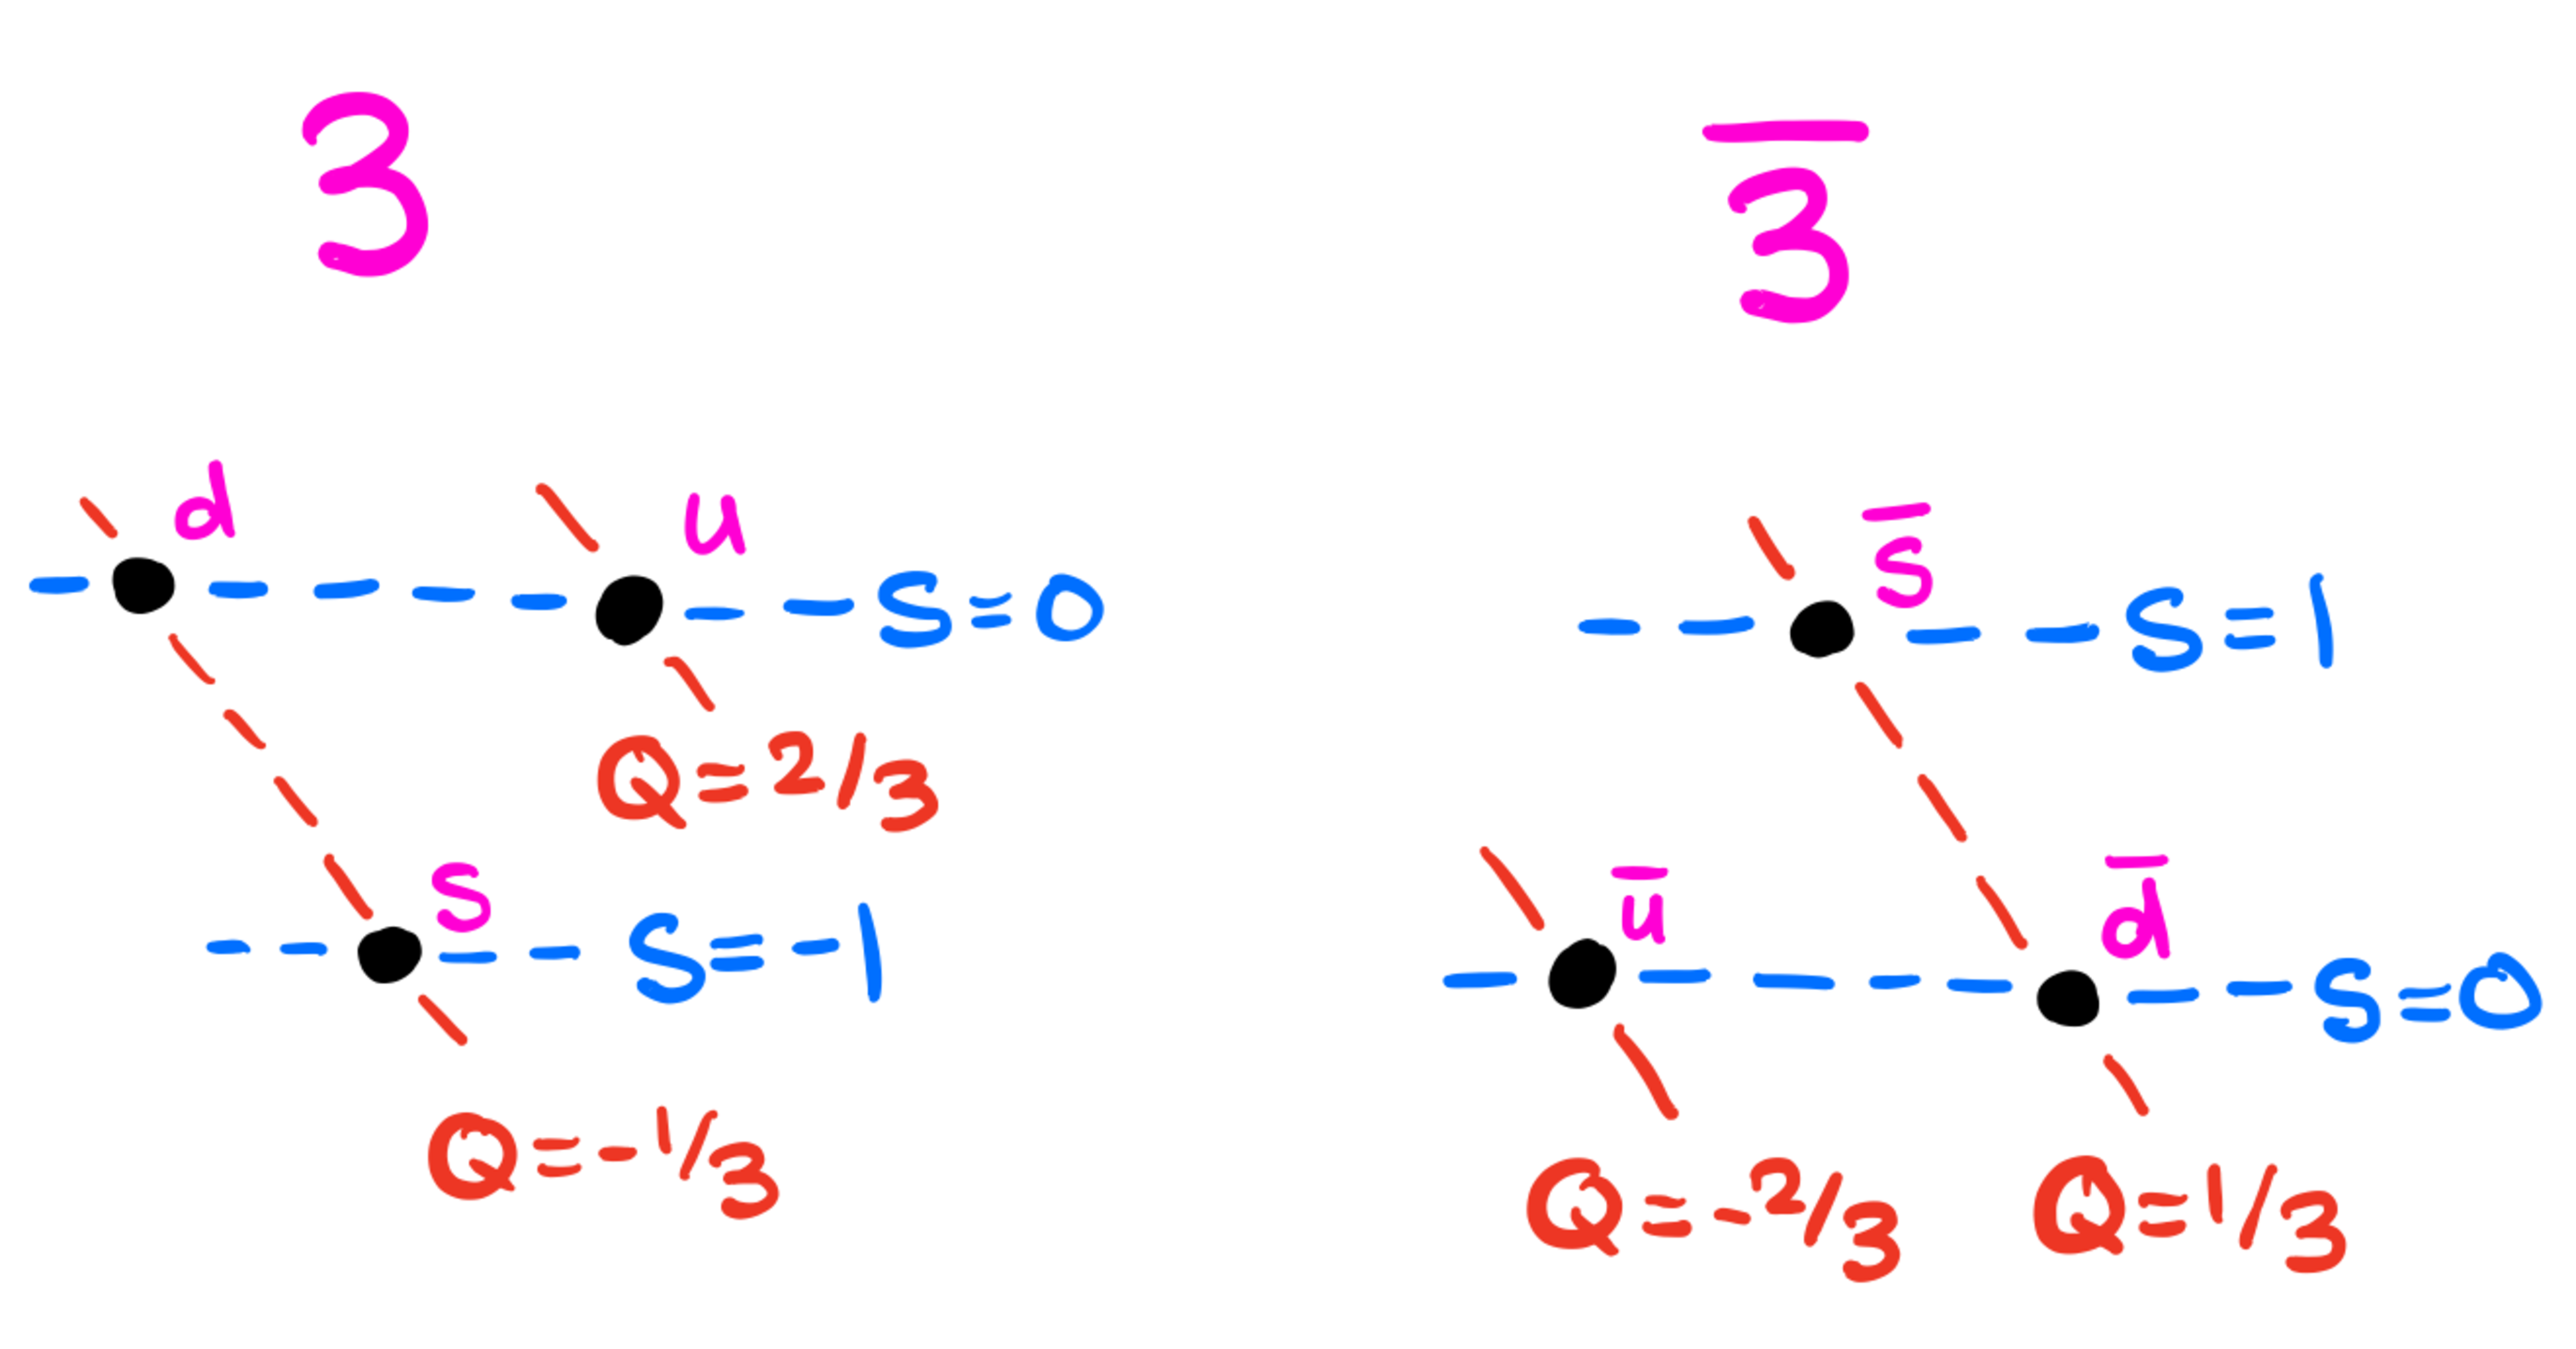
\includegraphics[width = .5\textwidth]{quark_weights}
		\caption{Weight diagram for fundamental and antifundamental of $SU(3)_f$.}
	\end{figure}
	
	\item Weight diagrams of light hadron multiplets of $SU(3)_f$:
	\begin{figure}[H]
	\centering
	\begin{subfigure}[t]{.38\textwidth}
		\centering
		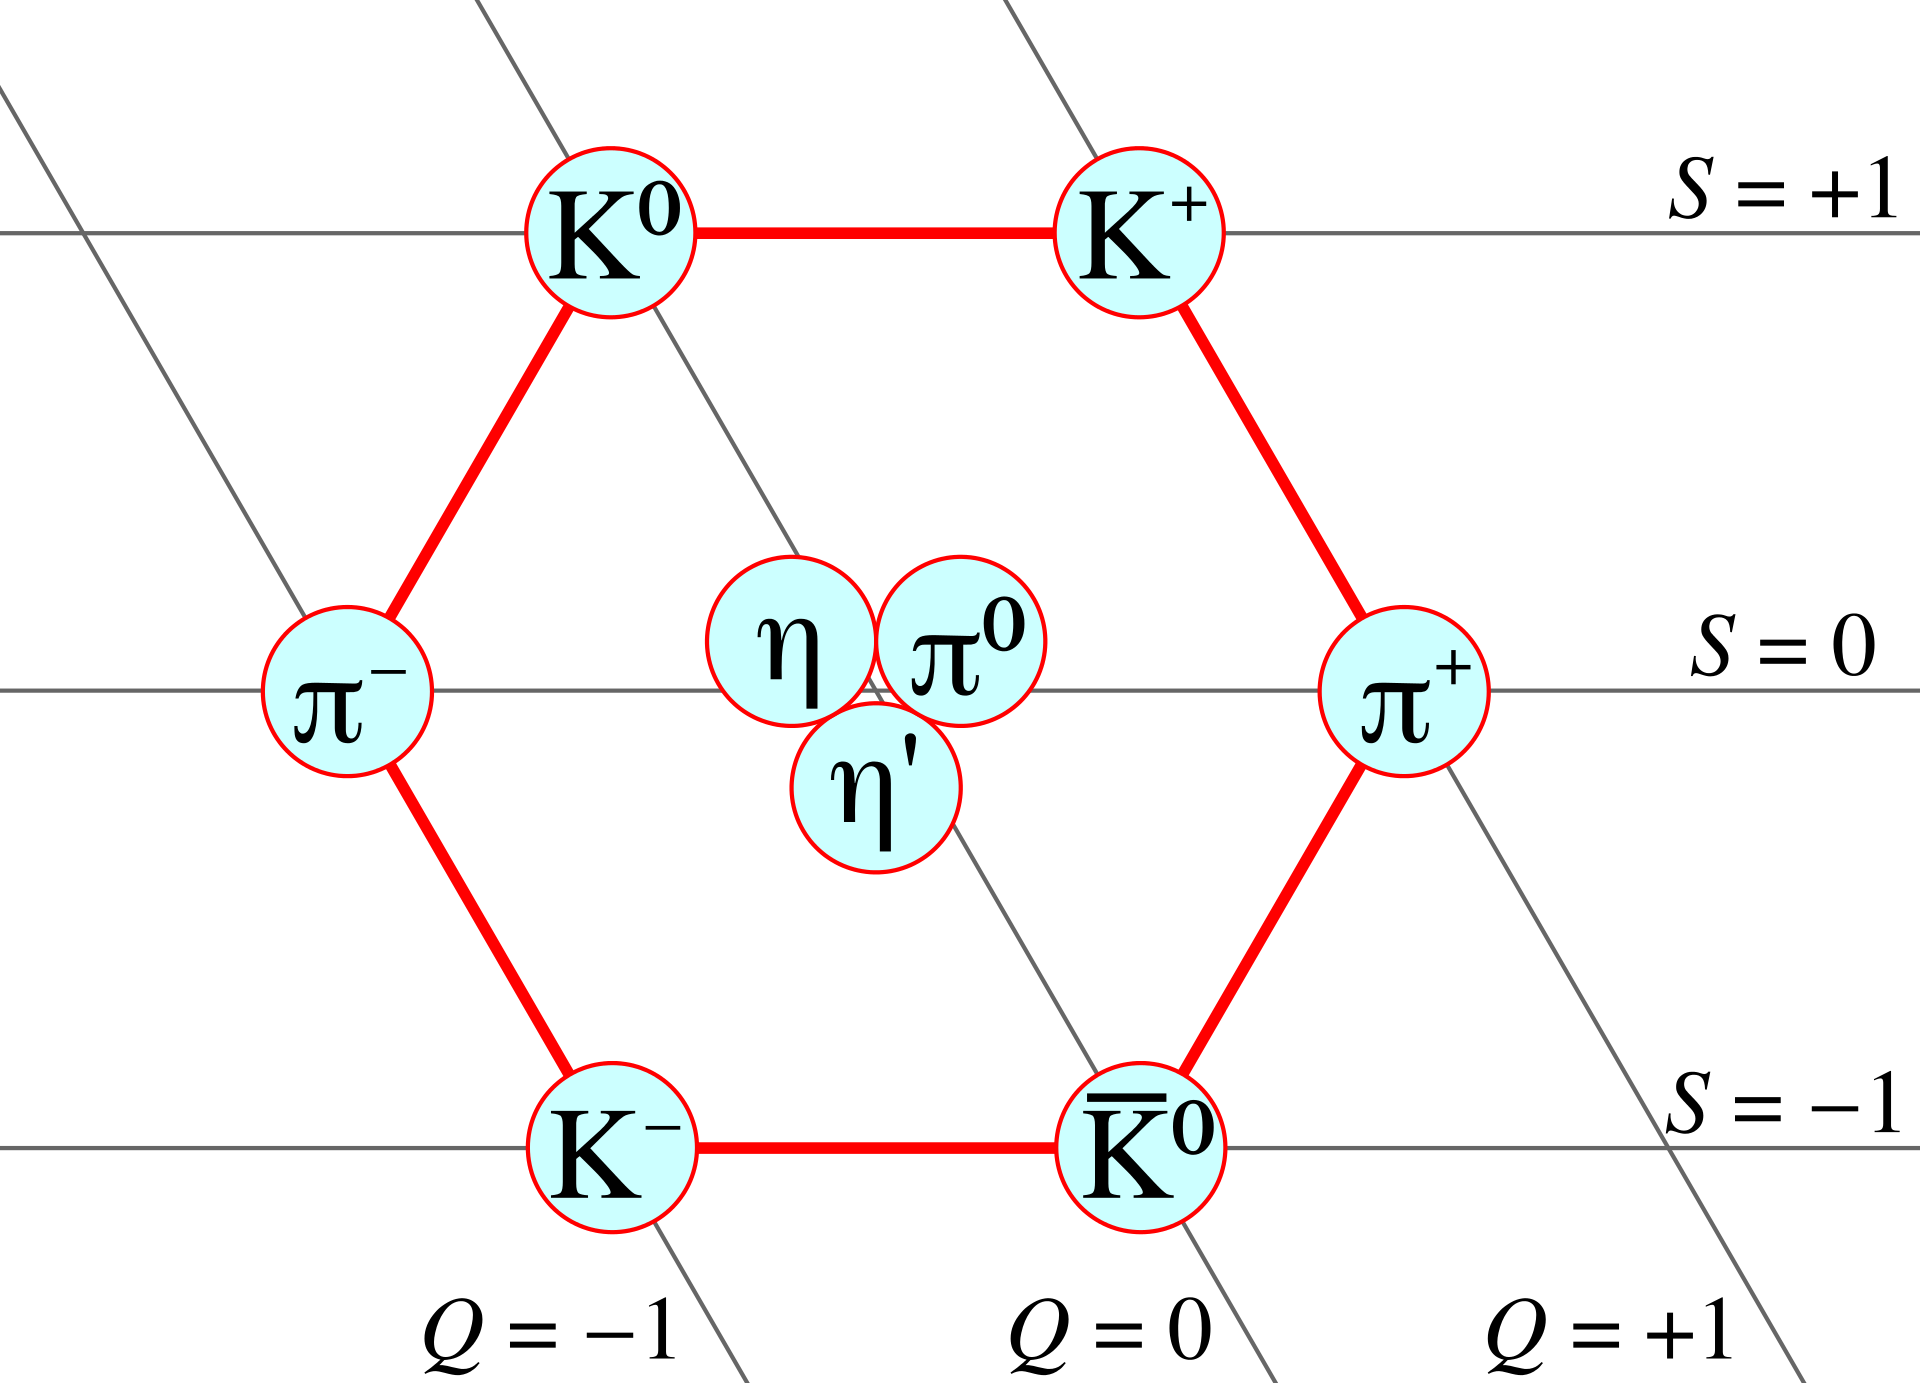
\includegraphics[width = .8\textwidth]{scalar_meson_nonet}
		\caption{Pseudoscalar meson nonet, $J^{PC} = 0^{-+}$.}~
	\end{subfigure}
	~
	\begin{subfigure}[t]{.38\textwidth}
		\centering
		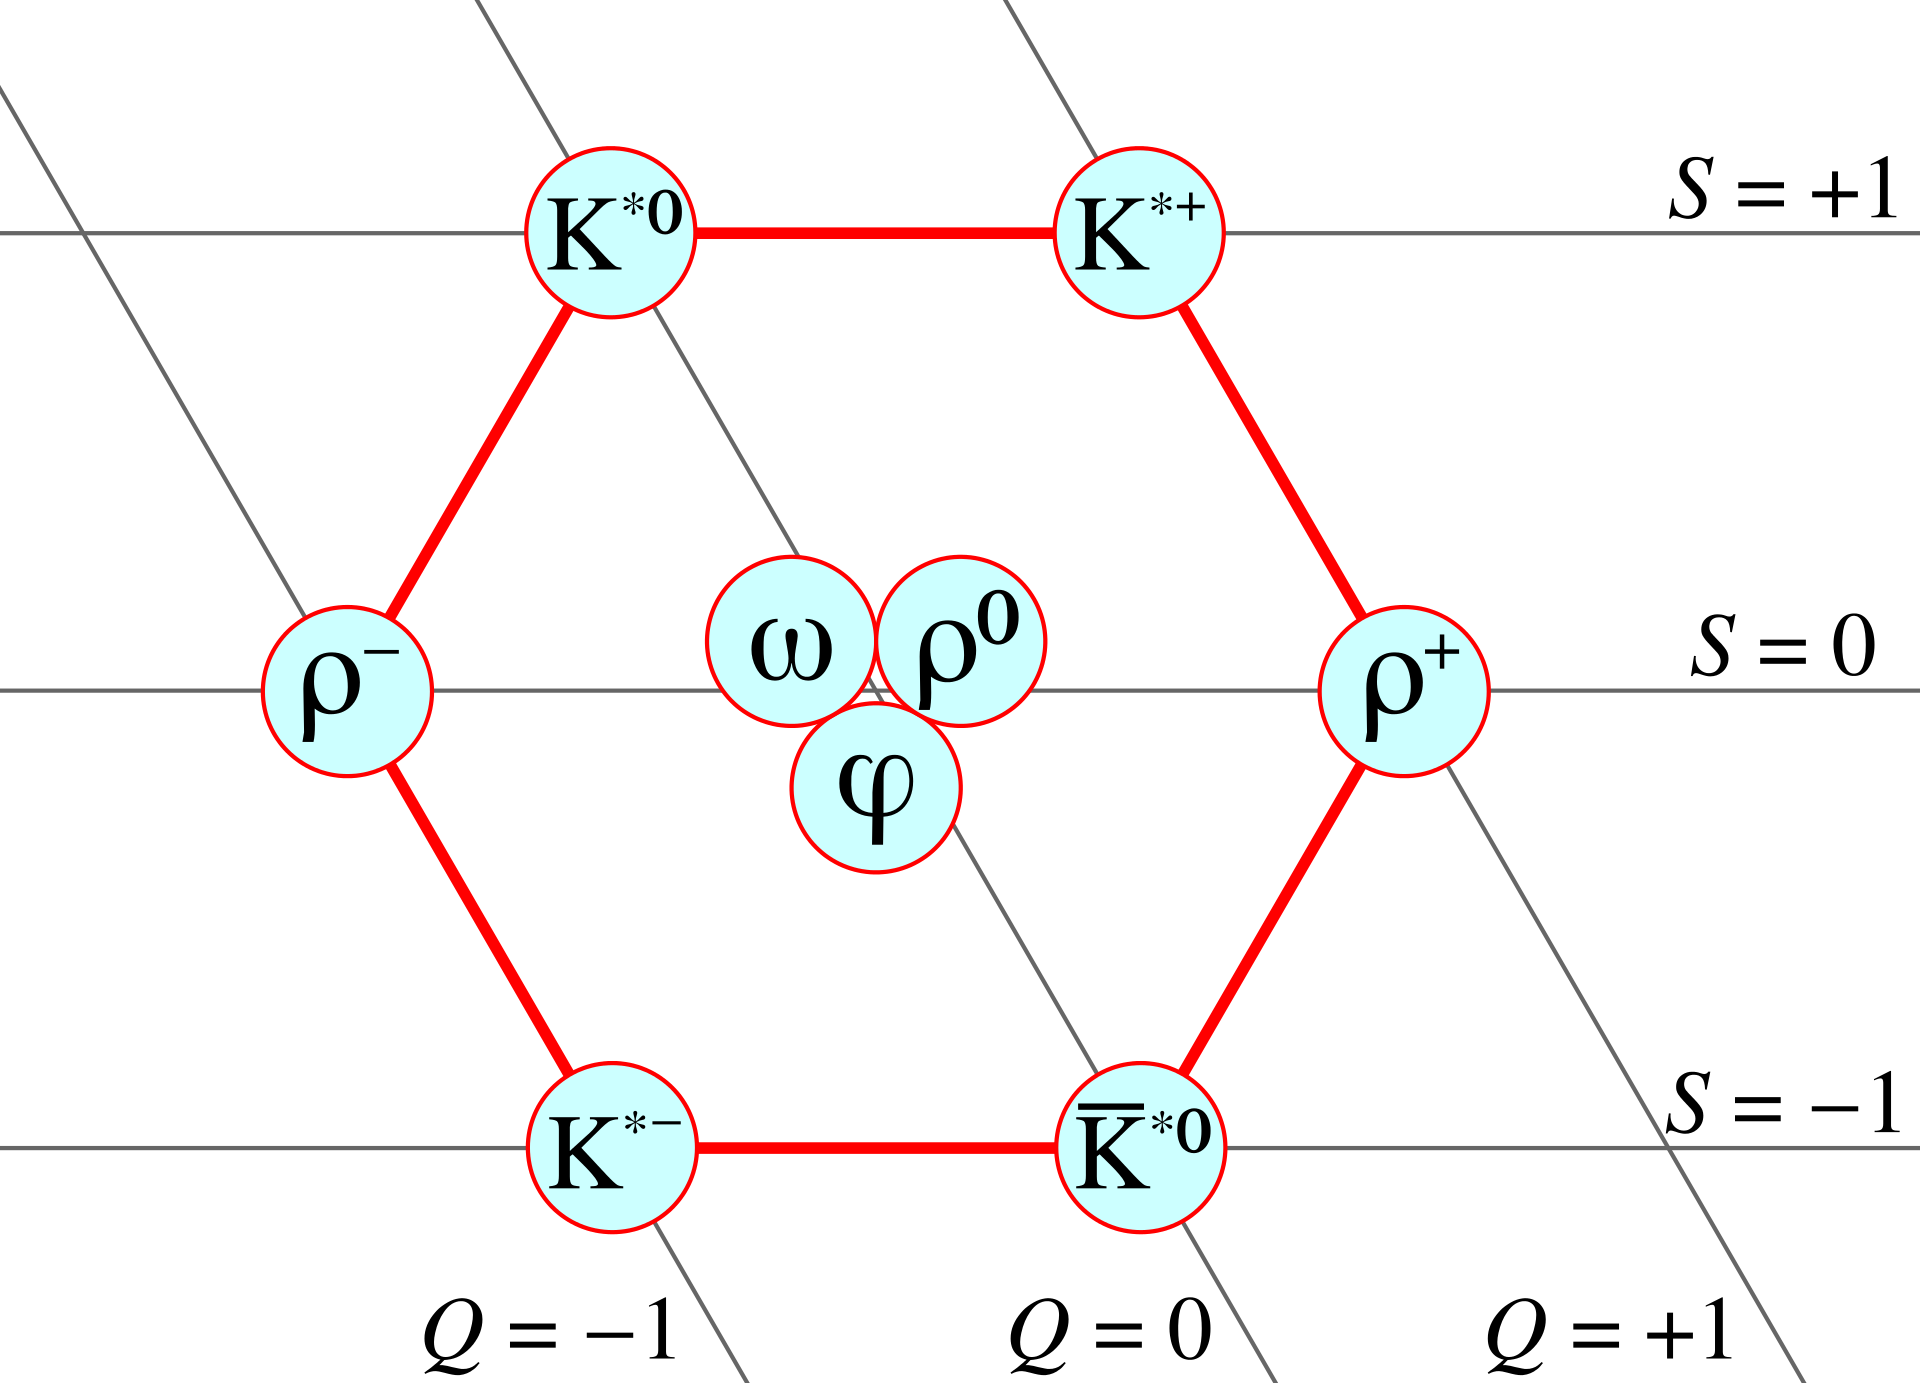
\includegraphics[width = .8\textwidth]{vector_meson_nonet}
		\caption{Pseudovector meson nonet, $J^{PC} = 1^{--}$}~
	\end{subfigure}
	\\
		\begin{subfigure}[t]{.38\textwidth}
		\centering
		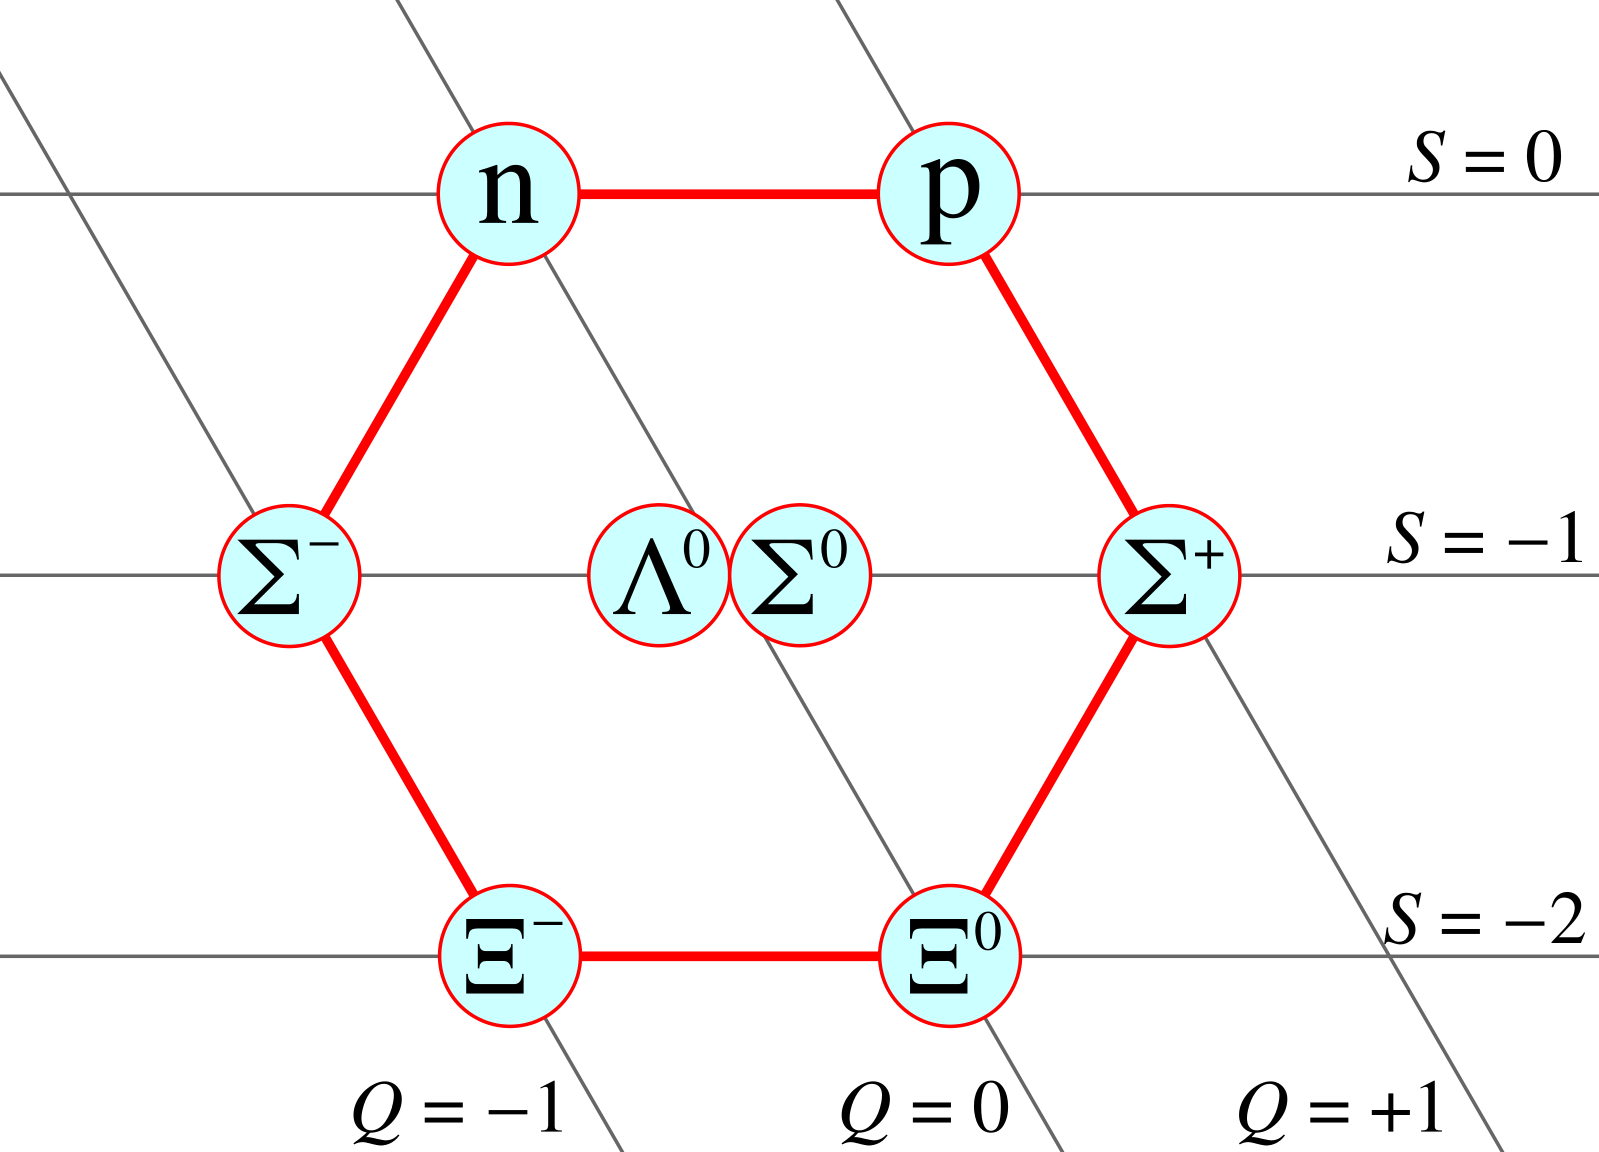
\includegraphics[width = .8\textwidth]{baryon_octet}
		\caption{Baryon octet, spin $\frac{1}{2}$, mixed flavor/spin symmetry, $J^P = \frac{1}{2}^+$.}~
	\end{subfigure}
	~
	\begin{subfigure}[t]{.38\textwidth}
		\centering
		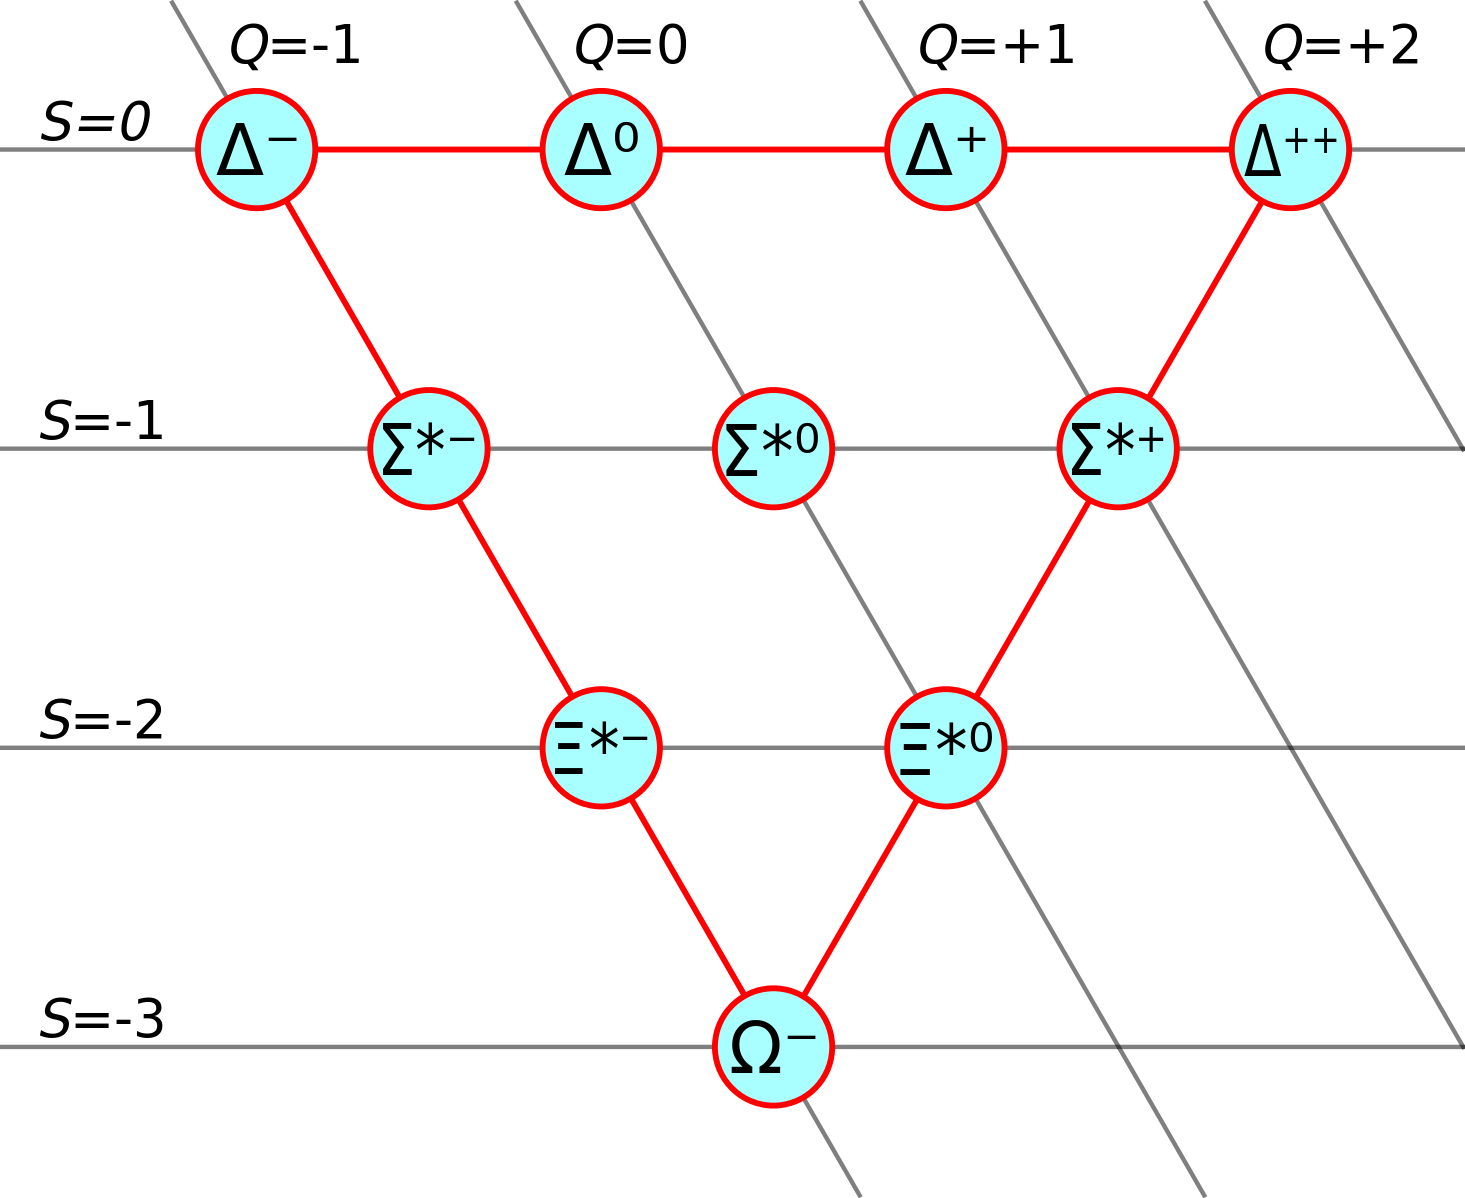
\includegraphics[width = .8\textwidth]{baryon_decuplet}
		\caption{Baryon decuplet, spin $\frac{3}{2}$, symmetric flavor / spin, $J^P = \frac{3}{2}^+$.}~
	\end{subfigure}
	\end{figure}
	
	\item \textbf{Approximate light hadron masses}: Each $SU(3)_f$ multiplet will be split in mass. Inside each of these multiplets, the isospin multiplets will be further 
	split by about $m_s / \Lambda_c\approx 20\;\%$ (about 150 MeV for anything other than a pion) and each isospin multiplet will be nearly degenerate in mass, splitting by isospin 
	breaking effects of about $m_d / \Lambda_c\approx 1\;\%$. 
	
	\item \textbf{Quantum numbers}: $C$ and $P$ are each individually conserved under $U(1)_\mathrm{EM}$ and $SU(3)_c$, but 
	electroweak interactions break $C$, $P$, and $CP$ (anything which has a CKM matrix element in it may break $CP$). For two particles in a 
	state with angular momentum $\ell$, their parity is:
	\begin{equation}
		P(ab) = (-1)^\ell P(a) P(b)
	\end{equation}
	\textbf{Mesons} with spin $s$, ang. momentum $\ell$, and constituent quark spin $j$ have
	\begin{align}
		C = (-1)^{\ell + s} && P = (-1)^{2j + \ell}
	\end{align}
	\textbf{Photons} and other gauge bosons are odd under $P$ and $C$:
	\begin{align}
		P |\gamma\rangle = - |\gamma\rangle
	\end{align}
	
	\item \textbf{Chiral Lagrangian}: Note $[\Sigma] = 0$ and $[\pi] = 1$:
	\begin{align}
		\Sigma = \exp\left(\frac{2i}{f_\pi} \pi^a(x) t^a\right) && \pi(x) =\frac{1}{\sqrt 2} \begin{pmatrix} \frac{1}{\sqrt 2} \pi^0 + \frac{1}{\sqrt 6} \eta & \pi^+ & K^+ \\ \pi^- & -\frac{1}{\sqrt 2} + \frac{1}{\sqrt 6} \eta & K^0 \\ K^- & \overline{K}^0 & -\frac{2}{\sqrt 6} \eta  \end{pmatrix}
	\end{align}
	Lagrangian and pion decay constant:
	\begin{align}
		\mathcal L_\chi = \frac{f_\pi^2}{4} tr\left\{\partial_\mu\Sigma \partial^\mu\Sigma^\dagger\right\} + \mu\,tr\left\{M_q\Sigma^\dagger + 
		M_q^\dagger\Sigma\right\} &&
		f_\pi = \textnormal{92 MeV}
	\end{align}
	Nucleon coupling: Add in a Dirac fermion $N$ by coupling it to $\Sigma$ in an invariant way. Upon Taylor expanding, will get a axial $\pi^a NN$ coupling:
	\begin{equation}
		\Delta\mathcal L_\chi = \overline N i\slashed D N + m_N \left(\overline N_L\Sigma N_R + \overline N_R\Sigma^\dagger N_L\right)\sim \overline N(i\slashed D - m_N) 
		- \frac{2i m_N}{f_\pi} \pi^a \overline N \gamma_5 t^a N 
	\end{equation}
	
	\item Mass relations from $\chi$PT and how to derive them:
	
	\item \textbf{Deep inelastic scattering}: DIS has a virtual photon hitting a nucleus with energy $Q$ and shattering it into pieces, and the DIS limit is 
	$Q^2\rightarrow\infty$. Bjorken variable $x$ is momentum fraction $\xi$ in the lightcone frame:
	\begin{equation}
		x = \frac{Q^2}{2p\cdot q}
	\end{equation}
	and has $x\in [0, 1]$. Bjorken scaling: as $Q^2\rightarrow\infty$, observables become independent of $Q^2$ and only functions of $x$ (this is broken 
	by logarithmic corrections in $Q^2$ from DGLAP). 
	
	\item \textbf{Parton distribution functions}: $f_i(x)$ is the probability density that the photon in DIS strikes parton $i$ when it has Bjorken variable $x$. 
	Nonperturbative objects which are necessary for factorization. Two types of sum rules: first: quark content labels the bounds state, and second: 
	the sum of all momenta is 1. 
	\begin{align}
		\int_0^1 dx\; \left(f_q(x) - f_{\overline q}(x)\right) = N_q^\mathrm{val} && \sum_i \int_0^1 dx\; x f_i(x) = 1
	\end{align}
	i.e. in the proton, the first sum rule for $q = u$ is $N_q = 2$ valence quarks.
	% How do they affect cross sections?
	
	% Draw an example of the PDFs for the proton to get an idea for what they look like for different quark content
	
	\item $\Delta I = \frac{1}{2}$: 
	
	\newpage
	\subsection{Topological effects}
	
	\item Anomalies: 
	\begin{itemize}
		\item How to compute: what is an anomaly? Symmetry which is classical (leaves action invariant) but does not survive to the 
		quantum limit (changes path integral measure). Use 3 point functions to compute, i.e. triangle diagrams. 
		\item Gauge vs global: Gauge anomalies are an issue in your theory and make it sick and violate unitarity (Ward identity is 
		broken). Gauge anomalies therefore must cancel. However, global anomalies do not need to cancel and don't make your theory 
		violate unitarity. 
		\item Anomaly coefficients: 
		\begin{align}
			d_R^{abc} = 2\;\mathrm{tr}\left[t^a_R \{t_R^b, t_R^c\}\right]= A(R) d^{abc} && d^{abc} := d_\mathrm{fund}^{abc}
			\\
			A(R_1\oplus R_2) = A(R_1) + A(R_2) && A(R) = - A(\overline R)
		\end{align}
		\item \textbf{Evaluation of the chiral anomaly}: For gauge theory with a Dirac fermion $\Psi$ charged under $G$ in irrep $R$, the 
		chiral anomaly is an anomaly in the axial current $j_5^{\mu a} = \overline \Psi \gamma^\mu \gamma_5 t^a\Psi$, which 
		equals:
		\begin{align}
			\partial_\mu j^{\mu a}_5 &= -\frac{g^2}{16\pi^2} \epsilon^{\mu\nu\alpha\beta} \mathrm{tr}\left[ t_R^a F_{\mu\nu} 
			F_{\alpha\beta} \right] \\
			&= - A(R) \frac{g^2}{64\pi^2} d^{abc} \epsilon^{\mu\nu\alpha\beta} F_{\mu\nu}^b F_{\alpha\beta}^c
		\end{align}
		For chiral fermions, $\psi_L = \frac{1 - \gamma_5}{2}\Psi$ and $\psi_R = \frac{1 + \gamma_5}{2}\Psi$ makes it obvious that this 
		anomaly creates an axial current in the gauge current $j^{\mu a} = \psi\gamma^\mu t^a\psi$, which must cancel with the anomaly 
		cancellation conditions to make the theory consistent with unitarity. For a theory charged under gauge groups $\{G_i\}$ with 
		left-handed fermions $\{\chi_\ell\}$ and right-handed fermions $\{\xi_r\}$ transforming in irreps of each $G_i$, the gauge current 
		$j_i^{\mu a}$ for $G_i$ suffers from the mixed anomaly:
		\begin{align}
			\left(\partial_\mu j_i^{\mu a}\right)_{jk} &= \left(\sum_{\ell = 1}^{n_L} \mathcal A_{ijk}^{abc}(\chi_\ell) - \sum_{r = 1}^{n_R} \mathcal A_{ijk}^{abc}(\xi_r)\right)
			\frac{g^2}{128\pi^2} \epsilon^{\mu\nu\alpha\beta}F_{\mu\nu}^b F_{\alpha\beta}^c \\
			&= \left(\sum_{\ell = 1}^{n_L} A(R_\ell) - \sum_{r = 1}^{n_R} \mathcal A(R_r)\right)
			\frac{g^2}{128\pi^2} d^{abc} \epsilon^{\mu\nu\alpha\beta}F_{\mu\nu}^b F_{\alpha\beta}^c\bigg|_{i = j = k} \\
			\mathcal A_{ijk}^{abc}(\psi) &= 2\;\mathrm{tr}\left[t^a_{R_i(\psi)}, \{t^b_{R_j(\psi)}, t^c_{R_k(\psi)}\}\right]
		\end{align}
		where $j$ and $k$ are the gauge groups which $F_{\mu\nu}^b$ and $F_{\alpha\beta}^c$ live in, respectively.
		\item \textbf{Anomaly cancellation conditions} are derived by requiring that $\partial_\mu j^{\mu a} = 0$ for each current coupling 
		to a gauge field in the presence of any external gauge fields in the theory. For a theory with multiple gauge symmetries $\{G_i\}$, 
		this corresponds to $q_\mu \langle j_i^{\mu a}(q) j_j^{\nu b}(p) j_k^{\sigma c}(k)\rangle$ vanishing, which is computed with 
		Eq.~(\ref{eq:mixed_anomaly_cancellation}). All anomalies cancel if for each $i, j, k$, the \textbf{anomaly cancellation condition} is 
		satisfied:
			\begin{align}
				\sum_{\ell = 1}^{n_L} \mathcal A_{ijk}^{abc}(\chi_\ell) - \sum_{r = 1}^{n_R} \mathcal A_{ijk}^{abc}(\xi_r) = 0 
			\end{align}
		where $\{\chi_\ell\}$ and $\{\xi_r\}$ are the left and right handed fields in the theory and $\mathcal A_{ijk}^{abc} = 2\mathrm{tr}[t^a, \{t^b, t^c\}]$ is 
		the mixed anomaly coefficient.
		\item \textbf{Baryon and lepton number}: Baryon number and lepton number suffer from mixed $SU(2)_L^2 G$ and $U(1)_Y^2 G$ 
		anomalies for $G = U(1)_B$ or $G = U(1)_{L_i}$. Their difference $B - L$ is not anomalous when considered with mixed 
		gauge-gauge-($B - L$) anomalies, however suffers from a grav$^2 (B - L)$ anomaly unless right-handed neutrinos are added to 
		the Standard Model.
	\end{itemize}
	
	\newpage
	\subsection{Miscellaneous}
	
	\item Muon lifetime: This is a good expression to keep in mind because decays from $W$ exchange will be proportional to this, 
	with quark weak interactions being suppressed by the appropriate CKM matrix elements:
	\begin{align}
		\Gamma(\mu^-\rightarrow e^- \overline\nu_e \nu_\mu) = \frac{G_F^2 m_\mu^5}{192\pi^3} && \tau_\mu\approx 2\;\mu\mathrm{s}
		\label{eq:muon_lifetime2}
	\end{align}
	
	\item Flavor-changing weak decay widths: To approximate the width of a particle which decays via the weak interaction, there are a few 
	basic steps:
	\begin{enumerate}
		\item Identify final states. In the case of lepton $\ell$ decay, this will emit a $W^*$ and a neutrino, so the neutrino will be 
		in the final state. In the case of quark $q$ decay, this will emit a $W^*$ (or a real $W$ for the top quark) and quark of the 
		opposite type. The primary decay product will be the one which is not CKM suppressed, which can be read off by the 
		Wolfenstein parameterization (i.e. $s$ quarks will primarily decay to $u W^-$; it would prefer to decay to $c W^-$ from the 
		CKM parameterization
		\item The $W^*$ is virtual and can then decay into either a lepton pair, or a hadron pair, assuming there is enough 
		available energy. This follows the same rules as above: it will decay through any channel which is not CKM suppressed 
		such that it has enough available energy.
		\item If all the particles other than the decaying one are assumed to be massless, the width of the decay is approximately 
		given by taking the muon width $\Gamma_\mu$, Eq.~(\ref{eq:muon_lifetime2}), replacing $m_\mu$ with the 
		mass of the decaying particle, then multiplying by the number of available channels and the appropriate CKM matrix. 
		Remember that meson channels each have multiplicity 3 for color, and lepton channels have multiplicity 1.
	\end{enumerate}
	
	\item Pion decay modes: 
	\begin{itemize}
		\item Charged pions: Primary decay is $\pi^\pm\rightarrow\mu^\pm \nu_\mu$. Compute this through $\pi^\pm$ interacting with an axial current, which couples 
		to the muon via the 4 Fermi theory. \textbf{This can be used to measure the pion decay constant}.
		\item Neutral pions: Primary decay is $\pi^0\rightarrow\gamma\gamma$. The $\pi^0$ couples to the current $j_5^{\mu 3}$. This current corresponds 
		to the symmetry $U(1)_{A, 3} : Q\mapsto e^{i\theta t^3\gamma_5}$, which has a mixed anomaly with $U(1)_\mathrm{EM}$:
		\begin{equation}
			\partial_\mu j_5^{\mu 3} = \left(\frac{N_c}{3}\right) \frac{e^2}{32\pi^2}\epsilon^{\mu\nu\alpha\beta} F_{\mu\nu} F_{\alpha\beta} \propto 2\;\mathrm{tr}[t^3, \{Q_\mathrm{EM}, Q_\mathrm{EM}\}]
		\end{equation}
		Under this transformation, the anomaly causes the Lagrangian to change as $\mathcal L\mapsto \mathcal L - i\theta\partial_\mu j_5^{\mu 3}$. 
		This is the importance of the anomaly: if $\partial_\mu j_5^{\mu 3}$ was equal to 0, then $\mathcal L$ would be invariant and we would be forbidden 
		from adding a term linear in $\pi^0$ to $\mathcal L$, since $\pi^0\mapsto \pi^0 + f_\pi\theta$ under the $U(1)_{A, 3}$ transformation (this is a generic 
		statement about Goldstone bosons and the symmetries that they break. To add the anomaly's behavior to the chiral Lagrangian, we must therefore have 
		a term in $\mathcal L$ which is linear in $\pi^0$ and couples $\pi^0$ to $\partial_\mu j_5^{\mu 3}$ to enforce the desired transformation law, 
		$\mathcal L\supset \frac{1}{f_\pi} \pi^0\partial_\mu j_5^{\mu 3}$. \textit{Because of the anomaly, we are inherently forced to couple $\pi^0$ to the 
		electromagnetic field to ensure that the chiral Lagrangian also has this anomalous symmetry; if this term is not included, then $\mathcal L_\chi$ 
		retains $U(1)_{A, 3}$ symmetry, and this is not manifested in nature.}
		The Lagrangian contains the coupling:
		\begin{equation}
			\mathcal L_{\pi\gamma\gamma} = -\frac{i}{f_\pi}\left(\frac{N_c}{3}\right) \frac{e^2}{32\pi^2}\pi^0\epsilon^{\mu\nu\alpha\beta} F_{\mu\nu} F_{\alpha\beta}
		\end{equation}
		which leads to the decay width:
		\begin{equation}
			\Gamma(\pi^0\rightarrow\gamma\gamma) = \frac{\alpha^2}{64\pi^3}\left(\frac{N_c}{3}\right)^2\frac{m_\pi^3}{f_\pi^2}
		\end{equation}
		\textit{This provides a robust measurement the number of colors in QCD}.
	\end{itemize}
	
	\item The Ward identity: https://physics.stackexchange.com/questions/292596/why-does-the-ward-identity-hold-for-gauge-theories
	
	The Ward-Takahashi identity applies for any type of gauge theory, $U(1)$, non-abelian, or massive where the mass is gained from 
	spontaneous symmetry breaking. In this case, one must apply $k_\mu \mathcal M^\mu = 0$ to both the diagrams which result 
	from transverse polarizations, and the diagram which results from longitudinal (Goldstone mode) polarization, and can be used 
	to derive the Goldstone equivalence theorem. 
	
	\item Generators of the Lorentz group: 
	\begin{align}
		\mathcal J_{\mu\nu} = i(x_\mu\partial_\nu - x_\nu\partial_\mu) && J_i = \epsilon_{ijk} \mathcal J^{jk} && K_i = \mathcal J_{0i}
	\end{align}
	The Lorentz algebra decouples into a sum of $\mathfrak{su}(2)\oplus\mathfrak{su}(2)$ when we take each copy of $\mathfrak{su}(2)$ to 
	be generated by $J_\pm^i = \frac{1}{2}(J_i\pm i K_i)$. The Lorentz group is non-compact so its irreps are infinite dimensional-- the finite 
	dimensional part gives a vector in the irrep a spinor / tensor structure (think internal dof that can be rotated like a spinor) and the infinite 
	dimensional part gives the vector a wavefunction structure. This means that elements in an irrep can be written as 
	$\psi_a(x)$, where $a$ parameterizes the irrep of $\mathfrak{su}(2)\oplus \mathfrak{su}(2)$ that we are in and the $x$ dependence is the 
	infinite dimensional part. 
	
	\item Irreps of the Poincar\'e group: The Poincar\'e group is generated by $\{\mathcal J_{\mu\nu}, P_\mu\}$ where $P_\mu$ is the momentum 
	4-vector. This has two Casimirs $P^2$ and $W^2$, where $W$ is the \textbf{Pauli-Lubanski pseudovector}:
	\begin{equation}
		W^\mu := \frac{1}{2} \epsilon^{\mu\nu\alpha\beta} \mathcal J_{\nu\alpha} P_\beta
	\end{equation}
	For \textbf{massive particles}, $P^2$ and $W^2$ completely define its irrep:
	\begin{align}
		P^2 = m^2 && W^2 = m^2 s (s + 1)
	\end{align}
	so we see that massive particles organize themselves into irreps of the Poincar\'e group according to their mass and spin. 
	
	\item The \textbf{little group} is another method used to determine the irreps of the Poincar\'e group. There are two basic steps:
	\begin{itemize}
		\item Diagonalize $P^\mu = p^\mu$.
		\item For a representative $p^\mu$ for a particle, let $G_p$ be the set of all Lorentz transformations which fix $p_\mu$. Then $G_p = 
		G_{p'}$ for any two momenta related by boosts, and $G_p$ is called the \textbf{little group}. 
	\end{itemize}
	The idea behind the little group is that we can relate each momentum in an irrep by boosts, then we can characterize which boosts fix 
	one of the momenta that the particle can access. Some little groups to know are:
	\begin{itemize}
		\item Massive particle:Take $p = (m, 0, 0, 0)$, so the little group is rotations on the bottom component, which is $SO(3)$. This has the 
		same algebra as $SU(2)$, which means that the spin of a particle can be characterized by the irreps of $\mathfrak{su}(2)$, i.e. 
		$s\in \{0, \frac{1}{2}, 1, ...\}$. 
		\item Massless particle: Take $p = (\omega, 0, 0, \omega)$. The little group consists of the rotation $J_3$ and two other linear combinations 
		of boosts and rotations. The little group is $ISO(2)$, the Euclidean group for $\mathbb R^2$, and irreps of the Lorentz group can be 
		characterized by their \textbf{helicity}. 
	\end{itemize}
	
	\item OPE: TODO
	
\end{itemize}

\newpage
\begin{thebibliography}{99}

\bibitem{pdg}
M. Tanabashi et al. (Particle Data Group), Phys. Rev. D 98, 030001 (2018).

\bibitem{tong_cft}
Tong, D. Lectures on String Theory. (2012). \textit{4. Introducing Conformal Field Theory}.

\bibitem{trace_anomaly1}
Collins, J., Duncan, A., Joglekar, S. (1977). Trace and dilatation anomalies in gauge theories Physical Review D  16(2), 438-449. https://dx.doi.org/10.1103/physrevd.16.438.

\bibitem{trace_anomaly2}
Nielsen, N. (1977). The energy-momentum tensor in a non-Abelian quark gluon theory Nuclear Physics B  120(2), 212-220. https://dx.doi.org/10.1016/0550-3213(77)90040-2

\bibitem{coleman_instantons}
Coleman, S. (1985). Aspects of Symmetry. https://dx.doi.org/10.1017/cbo9780511565045.008

\bibitem{instanton_abc}

\bibitem{ellis}
R. Ellis et al. \textit{QCD and Collider Physics}. Cambridge University Press (1996).


\end{thebibliography}

\end{document}